\chapter{Computed torque control}
A \ac{CT} controller is a nonlinear controller, which linearises the error system and applies then a linear control law for the stabilisation of the closed loop system. As a first step, the tracking error system need to be defined:
\begin{gather*}
	\mathbf{e} = \mathbf{q}_D - \mathbf{q}\\
	\dot{\mathbf{e}} = \dot{\mathbf{q}}_D - \dot{\mathbf{q}}\\
	\ddot{\mathbf{e}} = \ddot{\mathbf{q}}_D - \ddot{\mathbf{q}}
	%\label{eq:eq1}
	\intertext{where:}
	\begin{tabular}{>{$}l<{$} @{${}:{}$} l}
	\mathbf{e} & error vector\\
	\mathbf{q}_D & vector with reference trajectories for each joint
	\end{tabular}\nonumber
\end{gather*}
Substituting the acceleration vector $\ddot{\mathbf{q}}$ with the robot dynamics (Equation \ref{eq:ch1_robotdynamics}) results in
\begin{equation*}
	\ddot{\mathbf{e}} = \ddot{\mathbf{q}}_D - \mathbf{M}^{-1}\left(\tau - \mathbf{v} - \mathbf{g}\right) + \mathbf{M}^{-1}\tau_D
\end{equation*}
Defining $\mathbf{u} = \ddot{\mathbf{q}}_D - \mathbf{M}^{-1}\left(\tau - \mathbf{v} - \mathbf{g}\right)$ and $\mathbf{w} = \mathbf{M}^{-1}\tau_D$ results in the following linear system
\begin{equation*}
	\left(\begin{array}{c}
		\dot{\mathbf{e}} \\ \ddot{\mathbf{e}}
	\end{array}\right) = \left(\begin{array}{cc}
	\mathbf{0} & \mathbf{I} \\
	\mathbf{0} & \mathbf{0} 
	\end{array}\right) \left(\begin{array}{c}
	\mathbf{e} \\ \dot{\mathbf{e}}
	\end{array}\right) + \left(\begin{array}{c}
	\mathbf{0} \\ \mathbf{I}
	\end{array}\right) \mathbf{u} + \left(\begin{array}{c}
	\mathbf{0} \\ \mathbf{I}
	\end{array}\right) \mathbf{w}
\end{equation*}
As the actual input of the robot arm is not the input $\mathbf{u}$, but the motor torque $\tau$, $\mathbf{u} = \ddot{\mathbf{q}}_D - \mathbf{M}^{-1}\left(\tau - \mathbf{v} - \mathbf{g}\right)$ needs to be solved for $\tau$:
\begin{equation}
	\tau = \mathbf{M}(\ddot{\mathbf{q}}_D - \mathbf{u}) + \mathbf{v} + \mathbf{g}
	\label{eq:ch2_ctlaw}
\end{equation}
Equation \ref{eq:ch2_ctlaw} shows the \ac{CT} control law for the inner feedforward loop. This is the linearising control law, which nullifies the nonlinear parts of the robot dynamics and reduces the system to a linear double integrator system. The dynamics of the closed loop can be defined by choosing a specific linear controller for $\mathbf{u}$. Figure \ref{fig:ch2_control_loop} shows a schematic of the implementation of a \ac{CT} controller, with the linearising feedforward controller and the linear control law in the outer loop.
\begin{figure}[H]
	\centering
	\begin{tikzpicture}[M/.style={draw,outer sep=0pt,thick}]

	\node [M,thick,minimum width=2.5cm,minimum height=2cm] (plant) at (0,0) {Robot};
	\node [M,thick,minimum width=1cm,minimum height=1cm] (inertia) at (-4,0) {$\mathbf{M}$};
	% \node [M,thick,minimum width=2.5cm,minimum height=1.5cm] (cont2) at (0,-2.5) {$C_2(s)$};
	\node [M, circle] (add1) at ($(plant.west) + (-1,0)$) {};
	\node [M, circle] (add2) at ($(inertia.west) + (-1,0)$) {};
	\node at ($(add2.south east) + (0.2, -0.2)$) {$-$};
	\node [circle] (out1) at ($(plant.east) + (1.0, 0.5)$) {};
	\node [circle] (out2) at ($(plant.east) + (1.5, -0.5)$) {};
	
	\node [M,thick,minimum width=1cm,minimum height=1cm] (cogr) at ($(add1.south) + (0, -1)$) {$\mathbf{n}$};
	\node [M,thick,minimum width=1cm,minimum height=1cm] (lincont) at ($(inertia.south |- cogr.south) + (0, -1)$) {$\mathbf{u}$};
	
	\node [circle] (split1) at ($(cogr.south) + (0.25, -0.8)$) {};
	\node [circle] (split2) at ($(cogr.south) + (-0.25, -1.2)$) {};
	
	\draw [latex-, thick] (plant.west) -- (add1.east);
	\draw [thick, -latex] ($(plant.east) + (0, 0.5)$) -- node [above] {$\mathbf{q}$} (out1.east) -- ($(out1.east) + (0.6,0)$);
	\draw [thick, -latex] ($(plant.east) + (0, -0.5)$) -- node [above] {$\dot{\mathbf{q}}$} (out2.east) -- ($(out2.east) + (0.1,0)$);
	\draw [-latex, thick] (cogr.north) -- (add1.south);
	% \draw [-latex, thick] (out.west) -- ++(1, 0);
	% \draw [thick] ($(out) + (0,0)$) -- (out |- cont2) -- (cont2.east)[-latex];
	% \draw [thick] (cont2.west) -- (add |- cont2) -- (add.south)[-latex];
	\draw [latex-, thick] (add2.west) -- node [above] {$\ddot{\mathbf{q}}_D$} ++(-1, 0);
	\draw [-latex, thick] (add2.east) -- (inertia.west);
	\draw [-latex, thick] (inertia.east) -- (add1.west);
	\draw [-latex, thick] (lincont.west) -| (add2.south);
	\draw [-latex, thick] ($(out1)+(0,0)$) |- ($(split1)+(0,0)$) -- ($(cogr.south) + (0.25, 0)$);
	\draw [-latex, thick] ($(out2)+(0,0)$) |- ($(split2)+(0,0)$) -- ($(cogr.south) + (-0.25, 0)$);
	\draw [-latex, thick] ($(split1)+(0,0)$) -- ($(lincont.east) + (0, 0.2)$);
	\draw [-latex, thick] ($(split2)+(0,0)$) -- ($(lincont.east) + (0, -0.2)$);
	\draw [-latex, thick] ($(out1)+(0,0)$) -- ++(0, 1.2) -| (inertia.north);
	\draw [-latex, thick] ($(lincont.south) - (0, 1)$) -- node [right] {$\mathbf{q}_D$, $\mathbf{\dot{q}}_D$} (lincont.south);
	
	\fill (out1) circle [radius=1.5pt];
	\fill (out2) circle [radius=1.5pt];
	\fill (split1) circle [radius=1.5pt];
	\fill (split2) circle [radius=1.5pt];
	
	\node (Dash) at (inertia.west) [draw, dashed,xshift =1.4cm,yshift=-0.6cm,minimum width=3cm,minimum height=2.8cm] {};
	\node at ($(Dash.north) + (0.2,0.5)$) {feedforward};
	\node at ($(Dash.north) + (0.2,0.2)$) {controller};
	\node at ($(lincont.south) + (-1.4,-0.2)$) {linear outer};
	\node at ($(lincont.south) + (-1.4,-0.6)$) {loop controller};
	
\end{tikzpicture}
	\caption{Control loop with implement computed torque controller}
	\label{fig:ch2_control_loop}
\end{figure}
In the following two sections, two different control laws for $\mathbf{u}$ are designed and the behaviour of the closed loop system is simulated. For the simulations, the following two reference trajectories are used:
\begin{align*}
	q_{1,D} &= 0.1 \sin(\pi t)\\
	q_{2,D} &= 0.1 \cos(\pi t)
\end{align*}

\section{PD controller for outer loop}
\label{sec:ch2_1}
As first step, a PD control law of the form
\begin{equation*}
\end{equation*}
\begin{gather*}
\mathbf{u} = -\mathbf{K}_d \dot{\mathbf{e}} - \mathbf{K}_p \mathbf{e}
\intertext{where:}
\begin{tabular}{>{$}l<{$} @{${}:{}$} l}
\mathbf{K}_d & diagonal matrix with derivative gains \\
\mathbf{K}_p & diagonal matrix with proportional gains
\end{tabular}\nonumber
\end{gather*}
To find the stability range for the two gains, the linear system for the $i^{th}$ joint is considered.
\begin{equation*}
	\left(\begin{array}{c}
	\dot{e}_i \\ \ddot{e}_i
	\end{array}\right) = \left(\begin{array}{cc}
	0 & 1 \\
	-k_d & -k_p 
	\end{array}\right) \left(\begin{array}{c}
	e_i \\ \dot{e}_i
	\end{array}\right) + \left(\begin{array}{c}
	0 \\ 1
	\end{array}\right) w_i
\end{equation*}
The characteristic polynomial of the closed loop is then given by:
\begin{equation*}
	\Delta(s) = s^2 + k_{d,i} s + k_{p,i} \overset{!}{=} 0
\end{equation*}
The roots of this polynomial are negative if all coefficients have the same sign. Therefore, the controlled system is stable if $k_{d,i}$ and $k_{p,i}$ are both chosen positive. To set the two parameters, the characteristic polynomial is compared with a general second order polynomial:
\begin{equation*}
	p(s) = s^2 + 2\zeta \omega_ns+{\omega_n}^2
\end{equation*}
By comparing the two polynomials, the parameters of the controller can be set with $k_{d,i} = 2\zeta\omega_n$ and $k_{p,i} = {\omega_n}^2$. $\zeta$ describes the damping factor and $\omega_n$ the undamped, natural frequency. For the first simulation of the controller, the damping factor is set to $\zeta = 1$. This results in a faster system response than by choosing $\zeta > 1$ and has no overshoot, compared with $\zeta < 1$. To show the effects of over- and under-damping, two additional simulations are done. For the frequency $\omega_n = 10\,\frac{rad}{s}$ is used. A last simulation shows the influence of disturbances on the control behaviour. Table \ref{tab:ch2_pdparams} shows the controller parameters and the according Figure numbers, which show the simulation results.
\begin{table}[H]
	\begin{center}
		\caption{Controller parameters for simulations witch PD outer loop controller}
		\label{tab:ch2_pdparams}
		\begin{tabular}{lllll}
			 & & & & According \\
			 & $k_{p,i}$ & $k_{d,i}$ & $\tau_D$ & Figure \\
			\midrule
			$\zeta = 1$: & 100 & 20 & $0\,\mathrm{N\,m}$ & \ref{fig:ch2_sim1} \\
			$\zeta = 0.1$: & 100 & 2 & $0\,\mathrm{N\,m}$ & \ref{fig:ch2_sim2} \\
			$\zeta = 10$: & 100 & 200 & $0\,\mathrm{N\,m}$ & \ref{fig:ch2_sim3} \\
			$\zeta = 1$: & 100 & 20 & $1\,\mathrm{N\,m}$ & \ref{fig:ch2_sim4} \\
			\bottomrule
		\end{tabular}
	\end{center}
\end{table}
Figure \ref{fig:ch2_sim1} shows the simulation results for the \ac{CT} controller with PD controller and critical damping. In the upper two plots, the angular positions $\mathbf{q}$ and the applied torques of both joints can be seen. Joint 1 has an average input torque of $30\,\mathrm{N\,m}$ and a peak torque of $80\mathrm{N\,m}$ at the beginning. The other joint has gets an average torque of $10\,\mathrm{N\,m}$ and a peak torque of $30\,\mathrm{N\,m}$ at the beginning. These values are very high and a very strong motor would be needed to be able to apply such torques. The bottom left sub-figure shows the tracking error of the two joints. The error of the first joint starts at zero, has a small peak of approximately $0.001\,\mathrm{rad}$, and then converges to zero at $0.5\,\mathrm{s}$. The second joint starts with an error of $0.1\,\mathrm{rad}$, which is caused by the cosine input signal. The error also converges to zero at approximately $0.5\,\mathrm{s}$. The last plot shows the velocity error, which also converges to zero for both joints.
\begin{figure}[H]
	\centering
	% This file was created by matlab2tikz v0.4.3.
% Copyright (c) 2008--2013, Nico Schlömer <nico.schloemer@gmail.com>
% All rights reserved.
% 
% The latest updates can be retrieved from
%   http://www.mathworks.com/matlabcentral/fileexchange/22022-matlab2tikz
% where you can also make suggestions and rate matlab2tikz.
% 
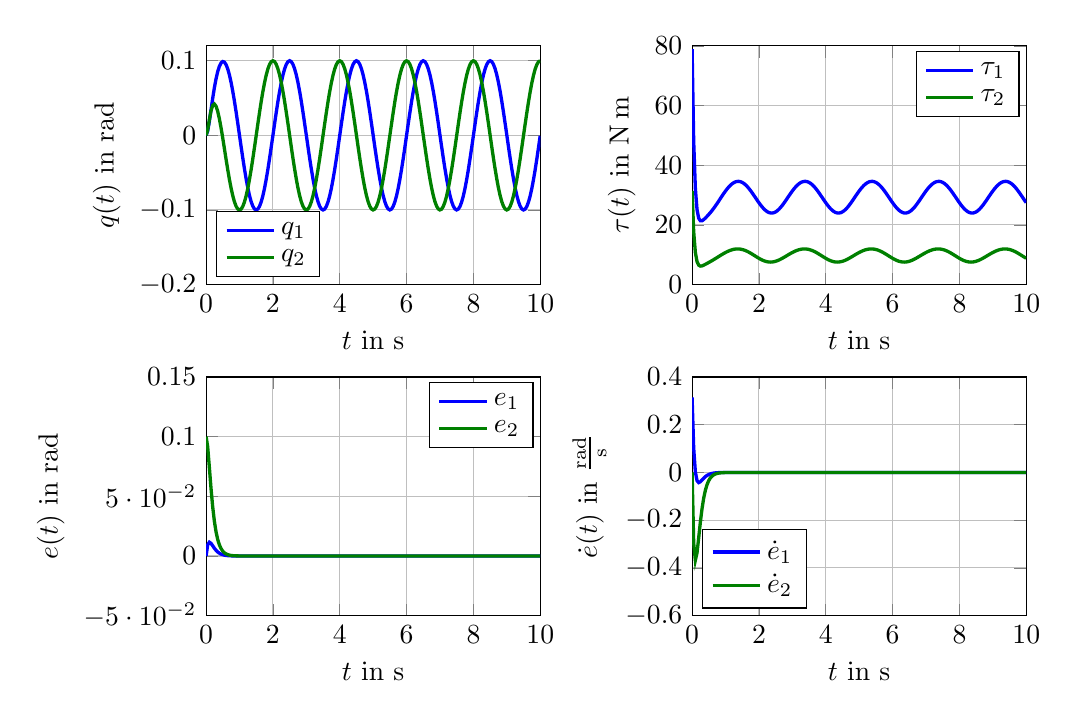
\begin{tikzpicture}

\begin{axis}[%
width=0.35\textwidth,
height=0.25\textwidth,
scale only axis,
xmin=0,
xmax=10,
xlabel={$t$ in $\mathrm{s}$},
xmajorgrids,
ymin=-0.2,
ymax=0.12,
ylabel={$q(t)$ in $\mathrm{rad}$},
ymajorgrids,
name=plot1,
legend style={at={(0.03,0.03)},anchor=south west,draw=black,fill=white,legend cell align=left}
]
\addplot [
color=blue,
solid,
line width=1.2pt
]
table[row sep=crcr]{
0 0\\
0.0476911628767132 0.00562695547618209\\
0.0976911628767132 0.0186569055696196\\
0.147691162876713 0.0341568483941079\\
0.197691162876713 0.049588647427124\\
0.247691162876713 0.0636593365391068\\
0.297691162876713 0.0757082664292471\\
0.347691162876713 0.0853934981885426\\
0.397691162876713 0.092537234252549\\
0.447691162876714 0.0970538348529895\\
0.497691162876714 0.0989192557520394\\
0.547691162876714 0.0981601001949206\\
0.597691162876714 0.0948509839948258\\
0.647691162876714 0.0891145419227714\\
0.697691162876714 0.0811213728758921\\
0.747691162876714 0.0710887574516762\\
0.797691162876714 0.0592777571325991\\
0.847691162876714 0.0459886837255253\\
0.897691162876714 0.031555105574433\\
0.947691162876714 0.0163366352588997\\
0.997691162876714 0.000710773969264721\\
1.04769116287671 -0.014935903958525\\
1.0976911628767 -0.030216944910402\\
1.1476911628767 -0.0447553142038671\\
1.19769116287669 -0.0581925355335868\\
1.24769116287669 -0.0701974227183508\\
1.29769116287668 -0.0804741723278495\\
1.34769116287668 -0.088769606796207\\
1.39769116287667 -0.0948793822160321\\
1.44769116287666 -0.0986530030039406\\
1.49769116287666 -0.0999975166952691\\
1.54769116287665 -0.0988797957516903\\
1.59769116287665 -0.0953273488032753\\
1.64769116287664 -0.0894276404466016\\
1.69769116287664 -0.0813259357647971\\
1.74769116287663 -0.0712217222696222\\
1.79769116287663 -0.0593637971288436\\
1.84769116287662 -0.0460441404939761\\
1.89769116287662 -0.0315907256894091\\
1.94769116287661 -0.0163594432375889\\
1.9976911628766 -0.000725337538000061\\
2.0476911628766 0.0149266280430691\\
2.09769116287659 0.0302110502936837\\
2.14769116287659 0.0447515760909241\\
2.19769116287658 0.0581901694816695\\
2.24769116287658 0.0701959277271888\\
2.29769116287657 0.0804732292337541\\
2.34769116287657 0.0887690127417524\\
2.39769116287656 0.0948790085364811\\
2.44769116287655 0.098652768248154\\
2.49769116287655 0.0999973693911318\\
2.54769116287654 0.09887970342457\\
2.59769116287654 0.0953272909949848\\
2.64769116287653 0.0894276042868546\\
2.69769116287653 0.0813259131672934\\
2.74769116287652 0.0712217081598977\\
2.79769116287652 0.0593637883260452\\
2.84769116287651 0.0460441350063254\\
2.89769116287651 0.0315907222709267\\
2.9476911628765 0.0163594411095596\\
2.99769116287649 0.000725336214164626\\
3.04769116287649 -0.0149266288660996\\
3.09769116287648 -0.0302110508050542\\
3.14769116287648 -0.0447515764084683\\
3.19769116287647 -0.0581901696787447\\
3.24769116287647 -0.0701959278494332\\
3.29769116287646 -0.0804732293095431\\
3.34769116287646 -0.0887690127887179\\
3.39769116287645 -0.0948790085655728\\
3.44769116287644 -0.0986527682661681\\
3.49769116287644 -0.0999973694022844\\
3.54769116287643 -0.0988797034314753\\
3.59769116287643 -0.0953272909992625\\
3.64769116287642 -0.0894276042895082\\
3.69769116287642 -0.0813259131689439\\
3.74769116287641 -0.0712217081609292\\
3.79769116287641 -0.0593637883266951\\
3.8476911628764 -0.0460441350067402\\
3.8976911628764 -0.0315907222711966\\
3.94769116287639 -0.01635944110974\\
3.99769116287638 -0.000725336214289435\\
4.0476911628764 0.01492662886601\\
4.09769116287642 0.030211050804988\\
4.14769116287643 0.0447515764084189\\
4.19769116287645 0.058190169678708\\
4.24769116287647 0.0701959278494065\\
4.29769116287648 0.0804732293095242\\
4.3476911628765 0.0887690127887048\\
4.39769116287652 0.0948790085655635\\
4.44769116287653 0.0986527682661605\\
4.49769116287655 0.0999973694022765\\
4.54769116287657 0.098879703431465\\
4.59769116287658 0.0953272909992479\\
4.6476911628766 0.0894276042894874\\
4.69769116287662 0.0813259131689156\\
4.74769116287663 0.0712217081608923\\
4.79769116287665 0.059363788326649\\
4.84769116287667 0.0460441350066847\\
4.89769116287668 0.0315907222711321\\
4.9476911628767 0.0163594411096674\\
4.99769116287672 0.000725336214210183\\
5.04769116287673 -0.0149266288660938\\
5.09769116287675 -0.0302110508050733\\
5.14769116287677 -0.0447515764085021\\
5.19769116287678 -0.058190169678786\\
5.2476911628768 -0.0701959278494761\\
5.29769116287682 -0.080473229309583\\
5.34769116287683 -0.0887690127887507\\
5.39769116287685 -0.0948790085655951\\
5.44769116287687 -0.0986527682661766\\
5.49769116287688 -0.0999973694022766\\
5.5476911628769 -0.0988797034314488\\
5.59769116287692 -0.0953272909992158\\
5.64769116287693 -0.0894276042894403\\
5.69769116287695 -0.0813259131688545\\
5.74769116287697 -0.0712217081608186\\
5.79769116287698 -0.0593637883265646\\
5.847691162877 -0.0460441350065916\\
5.89769116287702 -0.0315907222710326\\
5.94769116287703 -0.0163594411095639\\
5.99769116287705 -0.000725336214105265\\
6.04769116287707 0.0149266288661975\\
6.09769116287708 0.0302110508051733\\
6.1476911628771 0.044751576408596\\
6.19769116287712 0.0581901696788713\\
6.24769116287713 0.0701959278495508\\
6.29769116287715 0.0804732293096454\\
6.34769116287717 0.088769012788799\\
6.39769116287718 0.0948790085656282\\
6.4476911628772 0.0986527682661937\\
6.49769116287722 0.0999973694022772\\
6.54769116287723 0.0988797034314331\\
6.59769116287725 0.0953272909991841\\
6.64769116287727 0.0894276042893933\\
6.69769116287728 0.0813259131687934\\
6.7476911628773 0.071221708160745\\
6.79769116287732 0.0593637883264802\\
6.84769116287733 0.0460441350064985\\
6.89769116287735 0.031590722270933\\
6.94769116287737 0.0163594411094604\\
6.99769116287739 0.000725336214000362\\
7.0476911628774 -0.0149266288663013\\
7.09769116287742 -0.0302110508052733\\
7.14769116287744 -0.0447515764086898\\
7.19769116287745 -0.0581901696789566\\
7.24769116287747 -0.0701959278496256\\
7.29769116287749 -0.0804732293097076\\
7.3476911628775 -0.0887690127888474\\
7.39769116287752 -0.0948790085656614\\
7.44769116287754 -0.0986527682662109\\
7.49769116287755 -0.099997369402278\\
7.54769116287757 -0.0988797034314175\\
7.59769116287759 -0.0953272909991525\\
7.6476911628776 -0.0894276042893464\\
7.69769116287762 -0.0813259131687324\\
7.74769116287764 -0.0712217081606714\\
7.79769116287765 -0.0593637883263958\\
7.84769116287767 -0.0460441350064053\\
7.89769116287769 -0.0315907222708335\\
7.9476911628777 -0.0163594411093569\\
7.99769116287772 -0.000725336213895444\\
8.04769116287769 0.0149266288664047\\
8.09769116287767 0.0302110508053712\\
8.14769116287764 0.0447515764087783\\
8.19769116287761 0.058190169679033\\
8.24769116287758 0.0701959278496884\\
8.29769116287756 0.0804732293097568\\
8.34769116287753 0.088769012788884\\
8.3976911628775 0.0948790085656876\\
8.44769116287747 0.0986527682662297\\
8.49769116287744 0.0999973694022928\\
8.54769116287742 0.098879703431432\\
8.59769116287739 0.0953272909991705\\
8.64769116287736 0.0894276042893715\\
8.69769116287733 0.0813259131687678\\
8.74769116287731 0.0712217081607197\\
8.79769116287728 0.059363788326459\\
8.84769116287725 0.0460441350064843\\
8.89769116287722 0.0315907222709283\\
8.9476911628772 0.0163594411094667\\
8.99769116287717 0.00072533621401814\\
9.04769116287714 -0.0149266288662724\\
9.09769116287711 -0.0302110508052346\\
9.14769116287708 -0.0447515764086436\\
9.19769116287706 -0.0581901696789061\\
9.24769116287703 -0.0701959278495745\\
9.297691162877 -0.0804732293096603\\
9.34769116287697 -0.0887690127888084\\
9.39769116287695 -0.0948790085656356\\
9.44769116287692 -0.0986527682662032\\
9.49769116287689 -0.0999973694022929\\
9.54769116287686 -0.0988797034314588\\
9.59769116287683 -0.0953272909992236\\
9.64769116287681 -0.0894276042894498\\
9.69769116287678 -0.0813259131688693\\
9.74769116287675 -0.071221708160842\\
9.79769116287672 -0.0593637883265991\\
9.8476911628767 -0.0460441350066389\\
9.89769116287667 -0.0315907222710936\\
9.94769116287664 -0.0163594411096385\\
9.99769116287661 -0.000725336214192308\\
};
\addlegendentry{$q_1$};

\addplot [
color=green!50!black,
solid,
line width=1.2pt
]
table[row sep=crcr]{
0 0\\
0.0476911628767132 0.00720818578228093\\
0.0976911628767132 0.0209021053945203\\
0.147691162876713 0.0328693571254602\\
0.197691162876713 0.040096786929083\\
0.247691162876713 0.0420148662459838\\
0.297691162876713 0.0391014460581972\\
0.347691162876713 0.0322092680419061\\
0.397691162876713 0.0222622794473048\\
0.447691162876714 0.0101330310772948\\
0.497691162876714 -0.00339593862191369\\
0.547691162876714 -0.0176354197133027\\
0.597691162876714 -0.0319808479206076\\
0.647691162876714 -0.0459019403694645\\
0.697691162876714 -0.0589345597292393\\
0.747691162876714 -0.0706757233751423\\
0.797691162876714 -0.0807814049072269\\
0.847691162876714 -0.0889663417759846\\
0.897691162876714 -0.0950050092605669\\
0.947691162876714 -0.0987330215579193\\
0.997691162876714 -0.100048368500996\\
1.04769116287671 -0.0989120449293182\\
1.0976911628767 -0.0953477616993634\\
1.1476911628767 -0.0894405387318173\\
1.19769116287669 -0.0813340726908709\\
1.24769116287669 -0.0712268478459413\\
1.29769116287668 -0.0593670213593962\\
1.34769116287668 -0.0460461660891896\\
1.39769116287667 -0.0315919967324746\\
1.44769116287666 -0.016360239915929\\
1.49769116287666 -0.000725836367063153\\
1.54769116287665 0.0149263160144126\\
1.59769116287665 0.030210855292749\\
1.64769116287664 0.0447514543317625\\
1.69769116287664 0.0581900935171766\\
1.74769116287663 0.070195880370294\\
1.79769116287663 0.0804731997327125\\
1.84769116287662 0.0887689943768081\\
1.89769116287662 0.0948789971115039\\
1.94769116287661 0.0986527611450406\\
1.9976911628766 0.0999973649776327\\
2.0476911628766 0.0988797006838127\\
2.09769116287659 0.0953272892939116\\
2.14769116287659 0.0894276032316144\\
2.19769116287658 0.0813259125130096\\
2.24769116287658 0.0712217077544097\\
2.29769116287657 0.0593637880748581\\
2.34769116287657 0.0460441348507878\\
2.39769116287656 0.0315907221746537\\
2.44769116287655 0.0163594410499908\\
2.49769116287655 0.000725336177318265\\
2.54769116287654 -0.0149266288888848\\
2.59769116287654 -0.030211050819141\\
2.64769116287653 -0.0447515764171761\\
2.69769116287653 -0.0581901696841269\\
2.74769116287652 -0.0701959278527597\\
2.79769116287652 -0.0804732293115989\\
2.84769116287651 -0.0887690127899879\\
2.89769116287651 -0.0948790085663567\\
2.9476911628765 -0.0986527682666509\\
2.99769116287649 -0.0999973694025804\\
3.04769116287649 -0.098879703431655\\
3.09769116287648 -0.0953272909993696\\
3.14769116287648 -0.0894276042895695\\
3.19769116287647 -0.0813259131689763\\
3.24769116287647 -0.0712217081609432\\
3.29769116287646 -0.0593637883266973\\
3.34769116287646 -0.0460441350067347\\
3.39769116287645 -0.0315907222711862\\
3.44769116287644 -0.0163594411097266\\
3.49769116287644 -0.00072533621427441\\
3.54769116287643 0.0149266288660255\\
3.59769116287643 0.0302110508050025\\
3.64769116287642 0.0447515764084311\\
3.69769116287642 0.0581901696787173\\
3.74769116287641 0.0701959278494126\\
3.79769116287641 0.0804732293095278\\
3.8476911628764 0.0887690127887068\\
3.8976911628764 0.0948790085655654\\
3.94769116287639 0.098652768266164\\
3.99769116287638 0.0999973694022835\\
4.0476911628764 0.0988797034314772\\
4.09769116287642 0.0953272909992664\\
4.14769116287643 0.0894276042895125\\
4.19769116287645 0.0813259131689471\\
4.24769116287647 0.0712217081609297\\
4.29769116287648 0.0593637883266916\\
4.3476911628765 0.0460441350067315\\
4.39769116287652 0.031590722271182\\
4.44769116287653 0.0163594411097192\\
4.49769116287655 0.000725336214262663\\
4.54769116287657 -0.0149266288660419\\
4.59769116287658 -0.0302110508050233\\
4.6476911628766 -0.0447515764084552\\
4.69769116287662 -0.0581901696787433\\
4.74769116287663 -0.0701959278494388\\
4.79769116287665 -0.080473229309552\\
4.84769116287667 -0.0887690127887267\\
4.89769116287668 -0.0948790085655786\\
4.9476911628767 -0.0986527682661681\\
4.99769116287672 -0.0999973694022763\\
5.04769116287673 -0.0988797034314567\\
5.09769116287675 -0.0953272909992317\\
5.14769116287677 -0.0894276042894637\\
5.19769116287678 -0.0813259131688849\\
5.2476911628768 -0.0712217081608554\\
5.29769116287682 -0.0593637883266067\\
5.34769116287683 -0.0460441350066381\\
5.39769116287685 -0.0315907222710823\\
5.44769116287687 -0.0163594411096156\\
5.49769116287688 -0.000725336214157658\\
5.5476911628769 0.0149266288661457\\
5.59769116287692 0.0302110508051233\\
5.64769116287693 0.0447515764085491\\
5.69769116287695 0.0581901696788287\\
5.74769116287697 0.0701959278495135\\
5.79769116287698 0.0804732293096143\\
5.847691162877 0.0887690127887749\\
5.89769116287702 0.0948790085656116\\
5.94769116287703 0.0986527682661852\\
5.99769116287705 0.099997369402277\\
6.04769116287707 0.098879703431441\\
6.09769116287708 0.0953272909992\\
6.1476911628771 0.0894276042894168\\
6.19769116287712 0.0813259131688239\\
6.24769116287713 0.0712217081607818\\
6.29769116287715 0.0593637883265224\\
6.34769116287717 0.0460441350065451\\
6.39769116287718 0.0315907222709828\\
6.4476911628772 0.0163594411095122\\
6.49769116287722 0.00072533621405281\\
6.54769116287723 -0.0149266288662494\\
6.59769116287725 -0.0302110508052233\\
6.64769116287727 -0.0447515764086429\\
6.69769116287728 -0.058190169678914\\
6.7476911628773 -0.0701959278495882\\
6.79769116287732 -0.0804732293096765\\
6.84769116287733 -0.0887690127888232\\
6.89769116287735 -0.0948790085656447\\
6.94769116287737 -0.0986527682662023\\
6.99769116287739 -0.0999973694022777\\
7.0476911628774 -0.0988797034314254\\
7.09769116287742 -0.0953272909991683\\
7.14769116287744 -0.0894276042893699\\
7.19769116287745 -0.0813259131687629\\
7.24769116287747 -0.0712217081607082\\
7.29769116287749 -0.059363788326438\\
7.3476911628775 -0.046044135006452\\
7.39769116287752 -0.0315907222708833\\
7.44769116287754 -0.0163594411094087\\
7.49769116287755 -0.000725336213947885\\
7.54769116287757 0.0149266288663532\\
7.59769116287759 0.0302110508053233\\
7.6476911628776 0.0447515764087367\\
7.69769116287762 0.0581901696789993\\
7.74769116287764 0.0701959278496629\\
7.79769116287765 0.0804732293097388\\
7.84769116287767 0.0887690127888715\\
7.89769116287769 0.0948790085656779\\
7.9476911628777 0.0986527682662195\\
7.99769116287772 0.0999973694022784\\
8.04769116287769 0.0988797034314099\\
8.09769116287767 0.0953272909991387\\
8.14769116287764 0.0894276042893292\\
8.19769116287761 0.0813259131687151\\
8.24769116287758 0.0712217081606573\\
8.29769116287756 0.0593637883263881\\
8.34769116287753 0.0460441350064066\\
8.3976911628775 0.0315907222708455\\
8.44769116287747 0.0163594411093806\\
8.49769116287744 0.000725336213931007\\
8.54769116287742 -0.0149266288663585\\
8.59769116287739 -0.0302110508053177\\
8.64769116287736 -0.0447515764087215\\
8.69769116287733 -0.0581901696789769\\
8.74769116287731 -0.0701959278496365\\
8.79769116287728 -0.080473229309712\\
8.84769116287725 -0.0887690127888486\\
8.89769116287722 -0.0948790085656632\\
8.9476911628772 -0.0986527682662175\\
8.99769116287717 -0.0999973694022935\\
9.04769116287714 -0.0988797034314459\\
9.09769116287711 -0.0953272909991973\\
9.14769116287708 -0.0894276042894108\\
9.19769116287706 -0.0813259131688186\\
9.24769116287703 -0.0712217081607809\\
9.297691162877 -0.0593637883265291\\
9.34769116287697 -0.0460441350065617\\
9.39769116287695 -0.031590722271011\\
9.44769116287692 -0.0163594411095526\\
9.49769116287689 -0.000725336214105237\\
9.54769116287686 0.0149266288661863\\
9.59769116287683 0.0302110508051517\\
9.64769116287681 0.0447515764085658\\
9.69769116287678 0.0581901696788353\\
9.74769116287675 0.0701959278495124\\
9.79769116287672 0.0804732293096086\\
9.8476911628767 0.0887690127887683\\
9.89769116287667 0.0948790085656082\\
9.94769116287664 0.098652768266189\\
9.99769116287661 0.0999973694022923\\
};
\addlegendentry{$q_2$};

\end{axis}

\begin{axis}[%
width=0.35\textwidth,
height=0.25\textwidth,
scale only axis,
xmin=0,
xmax=10,
xlabel={$t$ in $\mathrm{s}$},
xmajorgrids,
ymin=-0.05,
ymax=0.15,
ylabel={$e(t)$ in $\mathrm{rad}$},
ymajorgrids,
name=plot3,
at=(plot1.below south west),
anchor=above north west,
legend style={draw=black,fill=white,legend cell align=left}
]
\addplot [
color=blue,
solid,
line width=1.2pt
]
table[row sep=crcr]{
0 0\\
0.0476911628767132 0.00929967338992492\\
0.0976911628767132 0.0115541452354623\\
0.147691162876713 0.0105947280143985\\
0.197691162876713 0.00860152225166256\\
0.247691162876713 0.00653659131036714\\
0.297691162876713 0.00476496288033226\\
0.347691162876713 0.00337551460020424\\
0.397691162876713 0.0023417743130436\\
0.447691162876714 0.00159893341318758\\
0.497691162876714 0.00107811365024225\\
0.547691162876714 0.000719603236539426\\
0.597691162876714 0.000476307004408774\\
0.647691162876714 0.000313062366696246\\
0.697691162876714 0.000204540292998975\\
0.747691162876714 0.000132950709188909\\
0.797691162876714 8.60311940217434e-05\\
0.847691162876714 5.54512811320115e-05\\
0.897691162876714 3.56166966737903e-05\\
0.947691162876714 2.28058507456587e-05\\
0.997691162876714 1.45622449274866e-05\\
1.04769116287671 9.27509241944839e-06\\
1.0976911628767 5.89410532312803e-06\\
1.1476911628767 3.73779536504137e-06\\
1.19769116287669 2.36585480568874e-06\\
1.24769116287669 1.49486888281758e-06\\
1.29769116287668 9.43018276161611e-07\\
1.34769116287668 5.94007465631874e-07\\
1.39769116287667 3.73650443794005e-07\\
1.44769116287666 2.34737765988924e-07\\
1.49769116287666 1.47292987542902e-07\\
1.54769116287665 9.23202274211166e-08\\
1.59769116287665 5.78040344478836e-08\\
1.64769116287664 3.61571240309333e-08\\
1.69769116287664 2.25958919491953e-08\\
1.74769116287663 1.41087390242989e-08\\
1.79769116287663 8.80220049626068e-09\\
1.84769116287662 5.48729277294324e-09\\
1.89769116287662 3.41827290778474e-09\\
1.94769116287661 2.12791121181888e-09\\
1.9976911628766 1.32377333552335e-09\\
2.0476911628766 8.23002319072508e-10\\
2.09769116287659 5.11362209520971e-10\\
2.14769116287659 3.17547016459585e-10\\
2.19769116287658 1.97083523112429e-10\\
2.24769116287658 1.22254567580526e-10\\
2.29769116287657 7.57987700383822e-11\\
2.34769116287657 4.69731059604683e-11\\
2.39769116287656 2.90962393068028e-11\\
2.44769116287655 1.80149922757167e-11\\
2.49769116287655 1.11495118693128e-11\\
2.54769116287654 6.8979960632376e-12\\
2.59769116287654 4.26651769469544e-12\\
2.64769116287653 2.63850052917292e-12\\
2.69769116287653 1.63183355716967e-12\\
2.74769116287652 1.00973396310877e-12\\
2.79769116287652 6.25555163225044e-13\\
2.84769116287651 3.88598875300517e-13\\
2.89769116287651 2.42326991806152e-13\\
2.9476911628765 1.52152596077926e-13\\
2.99769116287649 9.65717306469771e-14\\
3.04769116287649 6.24691270934008e-14\\
3.09769116287648 4.12586631526324e-14\\
3.14769116287648 2.80747647352086e-14\\
3.19769116287647 1.97411531566161e-14\\
3.24769116287647 1.45300438347817e-14\\
3.29769116287646 1.09079412169422e-14\\
3.34769116287646 8.31279489688086e-15\\
3.39769116287645 6.34214902817121e-15\\
3.44769116287644 4.8017145815038e-15\\
3.49769116287644 3.3584246494911e-15\\
3.54769116287643 2.08166817117217e-15\\
3.59769116287643 7.7715611723761e-16\\
3.64769116287642 -4.02455846426619e-16\\
3.69769116287642 -1.49880108324396e-15\\
3.74769116287641 -2.56739074444567e-15\\
3.79769116287641 -3.58740814832004e-15\\
3.8476911628764 -4.46864767411626e-15\\
3.8976911628764 -5.35682609381638e-15\\
3.94769116287639 -5.96050986345631e-15\\
3.99769116287638 -6.41348953112075e-15\\
4.0476911628764 -3.79904441238921e-16\\
4.09769116287642 4.94743135348585e-15\\
4.14769116287643 8.76382300063483e-15\\
4.19769116287645 1.11299858218672e-14\\
4.24769116287647 1.21708199074533e-14\\
4.29769116287648 1.2115308756222e-14\\
4.3476911628765 1.1143863609675e-14\\
4.39769116287652 9.47852907273727e-15\\
4.44769116287653 7.35522753814166e-15\\
4.49769116287655 4.8017145815038e-15\\
4.54769116287657 1.97064586870965e-15\\
4.59769116287658 -9.43689570931383e-16\\
4.6476911628766 -3.87190279838023e-15\\
4.69769116287662 -6.77236045021345e-15\\
4.74769116287663 -9.53404022396853e-15\\
4.79769116287665 -1.20875531806064e-14\\
4.84769116287667 -1.43565714871841e-14\\
4.89769116287668 -1.63133395680859e-14\\
4.9476911628767 -1.78572434617053e-14\\
4.99769116287672 -1.89473003259222e-14\\
5.04769116287673 -1.95711502559703e-14\\
5.09769116287675 -1.95468641273067e-14\\
5.14769116287677 -1.9373391779709e-14\\
5.19769116287678 -1.84158244209698e-14\\
5.2476911628768 -1.73194791841524e-14\\
5.29769116287682 -1.57235335862538e-14\\
5.34769116287683 -1.35585986882347e-14\\
5.39769116287685 -1.11577413974828e-14\\
5.44769116287687 -8.40993941153556e-15\\
5.49769116287688 -5.50948175970234e-15\\
5.5476911628769 -2.52575738102223e-15\\
5.59769116287692 5.96744875736022e-16\\
5.64769116287693 3.62210261783957e-15\\
5.69769116287695 6.77236045021345e-15\\
5.74769116287697 9.45077349712165e-15\\
5.79769116287698 1.21569421196455e-14\\
5.847691162877 1.43010603359528e-14\\
5.89769116287702 1.6382728507125e-14\\
5.94769116287703 1.7728873924483e-14\\
5.99769116287705 1.8996956785422e-14\\
6.04769116287707 1.94549237830799e-14\\
6.09769116287708 1.97793170730876e-14\\
6.1476911628771 1.92693083711504e-14\\
6.19769116287712 1.86031745563753e-14\\
6.24769116287713 1.72223346694977e-14\\
6.29769116287715 1.56263890715991e-14\\
6.34769116287717 1.34753319613878e-14\\
6.39769116287718 1.11577413974828e-14\\
6.4476911628772 8.451572774959e-15\\
6.49769116287722 5.59274848654923e-15\\
6.54769116287723 2.60902410786912e-15\\
6.59769116287725 -5.41233724504764e-16\\
6.64769116287727 -3.51108031537706e-15\\
6.69769116287728 -6.66133814775094e-15\\
6.7476911628773 -9.36750677027476e-15\\
6.79769116287732 -1.20181642415673e-14\\
6.84769116287733 -1.44745326835505e-14\\
6.89769116287735 -1.62439506290468e-14\\
6.94769116287737 -1.79647963172158e-14\\
6.99769116287739 -1.88840913392663e-14\\
7.0476911628774 -1.96821725584329e-14\\
7.09769116287742 -1.96509475358653e-14\\
7.14769116287744 -1.94427807187481e-14\\
7.19769116287745 -1.8471335572201e-14\\
7.24769116287747 -1.73333569719603e-14\\
7.29769116287749 -1.55708779203678e-14\\
7.3476911628775 -1.35447209004269e-14\\
7.39769116287752 -1.10744746706359e-14\\
7.44769116287754 -8.43769498715119e-15\\
7.49769116287755 -5.5649929109336e-15\\
7.54769116287757 -2.4980018054066e-15\\
7.59769116287759 5.68989300120393e-16\\
7.6476911628776 3.7470027081099e-15\\
7.69769116287762 6.59194920871187e-15\\
7.74769116287764 9.53404022396853e-15\\
7.79769116287765 1.19557141964322e-14\\
7.84769116287767 1.43565714871841e-14\\
7.89769116287769 1.61329283265843e-14\\
7.9476911628777 1.78398962269455e-14\\
7.99769116287772 1.8755721802044e-14\\
8.04769116287769 6.89379109353183e-15\\
8.09769116287767 -4.10435574416113e-15\\
8.14769116287764 -1.22332699525884e-14\\
8.19769116287761 -1.71945790938821e-14\\
8.24769116287758 -1.99285032920216e-14\\
8.29769116287756 -2.05530037433732e-14\\
8.34769116287753 -1.94705362943637e-14\\
8.3976911628775 -1.69725344889571e-14\\
8.44769116287747 -1.36279876272738e-14\\
8.49769116287744 -9.49240686054509e-15\\
8.54769116287742 -4.87110352054287e-15\\
8.59769116287739 -2.77555756156289e-17\\
8.64769116287736 5.07927033766009e-15\\
8.69769116287733 1.01169073118967e-14\\
8.74769116287731 1.4960255256824e-14\\
8.79769116287728 1.92137972199191e-14\\
8.84769116287725 2.33424390927439e-14\\
8.89769116287722 2.68812749837366e-14\\
8.9476911628772 2.97643854008101e-14\\
8.99769116287717 3.15725093638641e-14\\
9.04769116287714 3.29458682557515e-14\\
9.09769116287711 3.34975103211121e-14\\
9.14769116287708 3.32026073301961e-14\\
9.19769116287706 3.18356452311264e-14\\
9.24769116287703 2.9989899452687e-14\\
9.297691162877 2.74225087082414e-14\\
9.34769116287697 2.40363284831346e-14\\
9.39769116287695 1.99840144432528e-14\\
9.44769116287692 1.56125112837913e-14\\
9.49769116287689 1.07969189144796e-14\\
9.54769116287686 5.6621374255883e-15\\
9.59769116287683 5.27355936696949e-16\\
9.64769116287681 -4.71844785465692e-15\\
9.69769116287678 -9.86710713135608e-15\\
9.74769116287675 -1.48353551665537e-14\\
9.79769116287672 -1.9151347174784e-14\\
9.8476911628767 -2.32869279415127e-14\\
9.89769116287667 -2.67980082568897e-14\\
9.94769116287664 -2.96845881209151e-14\\
9.99769116287661 -3.14955310096177e-14\\
};
\addlegendentry{$e_1$};

\addplot [
color=green!50!black,
solid,
line width=1.2pt
]
table[row sep=crcr]{
0 0.1\\
0.0476911628767132 0.0916715176491792\\
0.0976911628767132 0.0744251856047144\\
0.147691162876713 0.0565582471640075\\
0.197691162876713 0.0412291262398082\\
0.247691162876713 0.0292068419148814\\
0.297691162876713 0.0202623422684238\\
0.347691162876713 0.0138348669647513\\
0.397691162876713 0.00932844282380213\\
0.447691162876714 0.00622641003235066\\
0.497691162876714 0.004121274836106\\
0.547691162876714 0.00270879084719557\\
0.597691162876714 0.00176979711552562\\
0.647691162876714 0.001150363960958\\
0.697691162876714 0.000744390050452681\\
0.747691162876714 0.000479795525668292\\
0.797691162876714 0.000308175597647467\\
0.847691162876714 0.000197328987237635\\
0.897691162876714 0.00012600069497426\\
0.947691162876714 8.02532917421467e-05\\
0.997691162876714 5.09990987146713e-05\\
1.04769116287671 3.23414978579128e-05\\
1.0976911628767 2.04707001278254e-05\\
1.1476911628767 1.29344423474148e-05\\
1.19769116287669 8.15952197577574e-06\\
1.24769116287669 5.13968507027951e-06\\
1.29769116287668 3.23303276712067e-06\\
1.34769116287668 2.03108252164186e-06\\
1.39769116287667 1.27446135483184e-06\\
1.44769116287666 7.98806268378222e-07\\
1.49769116287666 5.00152853752942e-07\\
1.54769116287665 3.12851675872763e-07\\
1.59769116287665 1.9551231333903e-07\\
1.64769116287664 1.22076724021203e-07\\
1.69769116287664 7.61615904787405e-08\\
1.74769116287663 4.74791616300596e-08\\
1.79769116287663 2.95768505242933e-08\\
1.84769116287662 1.84119253593407e-08\\
1.89769116287662 1.14540789492024e-08\\
1.94769116287661 7.12113121248414e-09\\
1.9976911628766 4.42464874461646e-09\\
2.0476911628766 2.74765273033939e-09\\
2.09769116287659 1.70533438759168e-09\\
2.14769116287659 1.05787087423259e-09\\
2.19769116287658 6.55905510460464e-10\\
2.24769116287658 4.06485622939101e-10\\
2.29769116287657 2.51798797090697e-10\\
2.34769116287657 1.55910832855266e-10\\
2.39769116287656 9.64988991492e-11\\
2.44769116287655 5.97039327698834e-11\\
2.49769116287655 3.69256966583492e-11\\
2.54769116287654 2.28304059685103e-11\\
2.59769116287654 1.41117048602091e-11\\
2.64769116287653 8.72048266931102e-12\\
2.69769116287653 5.38795397186931e-12\\
2.74769116287652 3.32860128349211e-12\\
2.79769116287652 2.0563273306351e-12\\
2.84769116287651 1.27042820707857e-12\\
2.89769116287651 7.84830533895331e-13\\
2.9476911628765 4.8480663927819e-13\\
2.99769116287649 2.99260616287711e-13\\
3.04769116287649 1.84394166602431e-13\\
3.09769116287648 1.1309009284588e-13\\
3.14769116287648 6.8736683012105e-14\\
3.19769116287647 4.10504963355152e-14\\
3.24769116287647 2.35367281220533e-14\\
3.29769116287646 1.24483756636096e-14\\
3.34769116287646 5.35682609381638e-15\\
3.39769116287645 8.04911692853238e-16\\
3.44769116287644 -2.30718222304915e-15\\
3.49769116287644 -4.20215078011932e-15\\
3.54769116287643 -5.37590805205213e-15\\
3.59769116287643 -6.05765437811101e-15\\
3.64769116287642 -6.49480469405717e-15\\
3.69769116287642 -6.47398801234544e-15\\
3.74769116287641 -6.24500451351651e-15\\
3.79769116287641 -5.80091530366644e-15\\
3.8476911628764 -5.17641485231479e-15\\
3.8976911628764 -4.413136522885e-15\\
3.94769116287639 -3.58046925441613e-15\\
3.99769116287638 -2.5951463200613e-15\\
4.0476911628764 -2.42861286636753e-15\\
4.09769116287642 -3.5527136788005e-15\\
4.14769116287643 -5.45397060847108e-15\\
4.19769116287645 -7.67441665772139e-15\\
4.24769116287647 -1.00613961606655e-14\\
4.29769116287648 -1.23581700428588e-14\\
4.3476911628765 -1.44884104713583e-14\\
4.39769116287652 -1.63202784619898e-14\\
4.44769116287653 -1.79752046580717e-14\\
4.49769116287655 -1.90324101964623e-14\\
4.54769116287657 -1.96336003011055e-14\\
4.59769116287658 -1.97723781791836e-14\\
4.6476911628766 -1.94150251431324e-14\\
4.69769116287662 -1.85892967685675e-14\\
4.74769116287663 -1.73194791841524e-14\\
4.79769116287665 -1.55708779203678e-14\\
4.84769116287667 -1.346145417358e-14\\
4.89769116287668 -1.10328413072125e-14\\
4.9476911628767 -8.34055047249649e-15\\
4.99769116287672 -5.41233724504764e-15\\
5.04769116287673 -2.44249065417534e-15\\
5.09769116287675 5.41233724504764e-16\\
5.14769116287677 3.62210261783957e-15\\
5.19769116287678 6.48092690624935e-15\\
5.2476911628768 9.4091401336982e-15\\
5.29769116287682 1.2115308756222e-14\\
5.34769116287683 1.42455491847215e-14\\
5.39769116287685 1.63480340376054e-14\\
5.44769116287687 1.77080572427712e-14\\
5.49769116287688 1.89953304821633e-14\\
5.5476911628769 1.9447984889176e-14\\
5.59769116287692 1.97758476261356e-14\\
5.64769116287693 1.92623694772465e-14\\
5.69769116287695 1.86170523441831e-14\\
5.74769116287697 1.72084568816899e-14\\
5.79769116287698 1.56263890715991e-14\\
5.847691162877 1.346145417358e-14\\
5.89769116287702 1.11577413974828e-14\\
5.94769116287703 8.39606162372775e-15\\
5.99769116287705 5.50948175970234e-15\\
6.04769116287707 2.4980018054066e-15\\
6.09769116287708 -6.10622663543836e-16\\
6.1476911628771 -3.59434704222394e-15\\
6.19769116287712 -6.66133814775094e-15\\
6.24769116287713 -9.36750677027476e-15\\
6.29769116287715 -1.20944920745103e-14\\
6.34769116287717 -1.42455491847215e-14\\
6.39769116287718 -1.63202784619898e-14\\
6.4476911628772 -1.76664238793478e-14\\
6.49769116287722 -1.89365667244146e-14\\
6.54769116287723 -1.93838001205648e-14\\
6.59769116287725 -1.96995197931926e-14\\
6.64769116287727 -1.91999194321113e-14\\
6.69769116287728 -1.85199078295284e-14\\
6.7476911628773 -1.71945790938821e-14\\
6.79769116287732 -1.56125112837913e-14\\
6.84769116287733 -1.36696209906972e-14\\
6.89769116287735 -1.11577413974828e-14\\
6.94769116287737 -8.46545056276682e-15\\
6.99769116287739 -5.52335954751015e-15\\
7.0476911628774 -2.42861286636753e-15\\
7.09769116287742 5.96744875736022e-16\\
7.14769116287744 3.76088049591772e-15\\
7.19769116287745 6.60582699651968e-15\\
7.24769116287747 9.54791801177635e-15\\
7.29769116287749 1.2038980923279e-14\\
7.3476911628775 1.44675937896466e-14\\
7.39769116287752 1.62231339473351e-14\\
7.44769116287754 1.79023462720806e-14\\
7.49769116287755 1.88022340752436e-14\\
7.54769116287757 1.96023752785379e-14\\
7.59769116287759 1.95884974907301e-14\\
7.6476911628776 1.94289029309402e-14\\
7.69769116287762 1.84643966782971e-14\\
7.74769116287764 1.73333569719603e-14\\
7.79769116287765 1.55292445569444e-14\\
7.84769116287767 1.35308431126191e-14\\
7.89769116287769 1.10605968828281e-14\\
7.9476911628777 8.46545056276682e-15\\
7.99769116287772 5.62050406216486e-15\\
8.04769116287769 4.24660306919122e-15\\
8.09769116287767 5.55111512312578e-15\\
8.14769116287764 8.49320613838245e-15\\
8.19769116287761 1.20459198171829e-14\\
8.24769116287758 1.6153745008296e-14\\
8.29769116287756 2.01852423664661e-14\\
8.34769116287753 2.39946951197112e-14\\
8.3976911628775 2.6999236180103e-14\\
8.44769116287747 2.97470381660503e-14\\
8.49769116287744 3.18377052152541e-14\\
8.54769116287742 3.31817906484844e-14\\
8.59769116287739 3.33864880186496e-14\\
8.64769116287736 3.31124017094453e-14\\
8.69769116287733 3.20368731543397e-14\\
8.74769116287731 3.0142555118573e-14\\
8.79769116287728 2.72837308301632e-14\\
8.84769116287725 2.4008572907519e-14\\
8.89769116287722 2.01089145335231e-14\\
8.9476911628772 1.5709655798446e-14\\
8.99769116287717 1.08107967022875e-14\\
9.04769116287714 5.74540415243519e-15\\
9.09769116287711 4.85722573273506e-16\\
9.14769116287708 -4.81559236931162e-15\\
9.19769116287706 -9.79771819231701e-15\\
9.24769116287703 -1.4738210651899e-14\\
9.297691162877 -1.93040028406699e-14\\
9.34769116287697 -2.34465225013025e-14\\
9.39769116287695 -2.66384136970999e-14\\
9.44769116287692 -2.95319324550292e-14\\
9.49769116287689 -3.16989273371759e-14\\
9.54769116287686 -3.30898503042576e-14\\
9.59769116287683 -3.33205685265625e-14\\
9.64769116287681 -3.30638294521179e-14\\
9.69769116287678 -3.19813620031084e-14\\
9.74769116287675 -3.00454106039183e-14\\
9.79769116287672 -2.72143418911242e-14\\
9.8476911628767 -2.39253061806721e-14\\
9.89769116287667 -2.00672811700997e-14\\
9.94769116287664 -1.56541446472147e-14\\
9.99769116287661 -1.08107967022875e-14\\
};
\addlegendentry{$e_2$};

\end{axis}

\begin{axis}[%
width=0.35\textwidth,
height=0.25\textwidth,
scale only axis,
xmin=0,
xmax=10,
xlabel={$t$ in $\mathrm{s}$},
xmajorgrids,
ymin=-0.6,
ymax=0.4,
ylabel={$\dot{e}(t)$ in $\mathrm{\frac{rad}{s}}$},
ymajorgrids,
name=plot2,
at=(plot3.right of south east),
anchor=left of south west,
legend style={at={(0.03,0.03)},anchor=south west,draw=black,fill=white,legend cell align=left}
]
\addplot [
color=blue,
solid,
line width=1.2pt
]
table[row sep=crcr]{
0 0.314159265358979\\
0.0476911628767132 0.10200109859159\\
0.0976911628767132 0.00273071162858196\\
0.147691162876713 -0.0342115864976095\\
0.197691162876713 -0.0425053249243441\\
0.247691162876713 -0.0389758262129946\\
0.297691162876713 -0.0316432319916454\\
0.347691162876713 -0.0240467755842322\\
0.397691162876713 -0.0175293188161858\\
0.447691162876714 -0.0124178242478847\\
0.497691162876714 -0.00861490625631435\\
0.547691162876714 -0.00588214730513155\\
0.597691162876714 -0.00396615847169872\\
0.647691162876714 -0.00264727236522794\\
0.697691162876714 -0.00175223554607515\\
0.747691162876714 -0.00115169208511684\\
0.797691162876714 -0.000752461686852612\\
0.847691162876714 -0.000489098325996196\\
0.897691162876714 -0.000316491075799896\\
0.947691162876714 -0.000203993863151342\\
0.997691162876714 -0.000131026504688825\\
1.04769116287671 -8.38980362833919e-05\\
1.0976911628767 -5.35715052745744e-05\\
1.1476911628767 -3.41211581755263e-05\\
1.19769116287669 -2.16832017402857e-05\\
1.24769116287669 -1.37505807170646e-05\\
1.29769116287668 -8.70349345399868e-06\\
1.34769116287668 -5.4993153081051e-06\\
1.39769116287667 -3.46917037967465e-06\\
1.44769116287666 -2.18523135901011e-06\\
1.49769116287666 -1.37458317692445e-06\\
1.54769116287665 -8.63551992365263e-07\\
1.59769116287665 -5.41860627964463e-07\\
1.64769116287664 -3.39627143020049e-07\\
1.69769116287664 -2.12649162861789e-07\\
1.74769116287663 -1.33014627423655e-07\\
1.79769116287663 -8.3125639926962e-08\\
1.84769116287662 -5.19031466694742e-08\\
1.89769116287662 -3.23814799418898e-08\\
1.94769116287661 -2.01866139359907e-08\\
1.9976911628766 -1.25751130064522e-08\\
2.0476911628766 -7.82813613930955e-09\\
2.09769116287659 -4.86987650205606e-09\\
2.14769116287659 -3.02764158188751e-09\\
2.19769116287658 -1.88118087773859e-09\\
2.24769116287658 -1.16817430728666e-09\\
2.29769116287657 -7.25013798996699e-10\\
2.34769116287657 -4.49733889018589e-10\\
2.39769116287656 -2.78833206523998e-10\\
2.44769116287655 -1.72790684538349e-10\\
2.49769116287655 -1.07026893424178e-10\\
2.54769116287654 -6.62632657077999e-11\\
2.59769116287654 -4.10080996937623e-11\\
2.64769116287653 -2.53700116470412e-11\\
2.69769116287653 -1.5691531407569e-11\\
2.74769116287652 -9.70493130303396e-12\\
2.79769116287652 -6.00441918408023e-12\\
2.84769116287651 -3.71835895407457e-12\\
2.89769116287651 -2.30754304553216e-12\\
2.9476911628765 -1.43757228343588e-12\\
2.99769116287649 -9.01667629449321e-13\\
3.04769116287649 -5.71709346530724e-13\\
3.09769116287648 -3.69038133385402e-13\\
3.14769116287648 -2.44249065417534e-13\\
3.19769116287647 -1.67088565206086e-13\\
3.24769116287647 -1.19404486298436e-13\\
3.29769116287646 -8.89011086968594e-14\\
3.34769116287646 -6.86950496486816e-14\\
3.39769116287645 -5.46923617505968e-14\\
3.44769116287644 -4.46170878021235e-14\\
3.49769116287644 -3.5905306505768e-14\\
3.54769116287643 -2.82135426132868e-14\\
3.59769116287643 -2.08444372873373e-14\\
3.64769116287642 -1.42663658664333e-14\\
3.69769116287642 -7.43849426498855e-15\\
3.74769116287641 -4.9960036108132e-16\\
3.79769116287641 6.55031584528842e-15\\
3.8476911628764 1.32671651442706e-14\\
3.8976911628764 1.93178806284777e-14\\
3.94769116287639 2.47024622979097e-14\\
3.99769116287638 2.96984659087229e-14\\
4.0476911628764 2.09277040141842e-14\\
4.09769116287642 -1.88737914186277e-15\\
4.14769116287643 -2.53130849614536e-14\\
4.19769116287645 -4.42423875313125e-14\\
4.24769116287647 -5.72042413438112e-14\\
4.29769116287648 -6.40598685208715e-14\\
4.3476911628765 -6.55864251797311e-14\\
4.39769116287652 -6.22973894692791e-14\\
4.44769116287653 -5.58789126081649e-14\\
4.49769116287655 -4.60833628201929e-14\\
4.54769116287657 -3.40769079620884e-14\\
4.59769116287658 -2.06640260458357e-14\\
4.6476911628766 -6.32827124036339e-15\\
4.69769116287662 8.52096171399808e-15\\
4.74769116287663 2.34534613952064e-14\\
4.79769116287665 3.78030939884866e-14\\
4.84769116287667 5.1458837191376e-14\\
4.89769116287668 6.40598685208715e-14\\
4.9476911628767 7.49955653134293e-14\\
4.99769116287672 8.41549052665869e-14\\
5.04769116287673 9.13158437754191e-14\\
5.09769116287675 9.6034291630076e-14\\
5.14769116287677 9.85322934354826e-14\\
5.19769116287678 9.83657599817889e-14\\
5.2476911628768 9.63118473862323e-14\\
5.29769116287682 9.1926466438963e-14\\
5.34769116287683 8.44602165983588e-14\\
5.39769116287685 7.58559881575138e-14\\
5.44769116287687 6.42610964440848e-14\\
5.49769116287688 5.22325238616617e-14\\
5.5476911628769 3.78586051397178e-14\\
5.59769116287692 2.37587727269784e-14\\
5.64769116287693 7.91033905045424e-15\\
5.69769116287695 -7.41073868937292e-15\\
5.74769116287697 -2.32036612146658e-14\\
5.79769116287698 -3.75810493835615e-14\\
5.847691162877 -5.18474152499948e-14\\
5.89769116287702 -6.42264019745653e-14\\
5.94769116287703 -7.50510764646606e-14\\
5.99769116287705 -8.40993941153556e-14\\
6.04769116287707 -9.10937991704941e-14\\
6.09769116287708 -9.61453139325386e-14\\
6.1476911628771 -9.84212711330201e-14\\
6.19769116287712 -9.86433157379452e-14\\
6.24769116287713 -9.59232693276135e-14\\
6.29769116287715 -9.14823772291129e-14\\
6.34769116287717 -8.40438829641244e-14\\
6.39769116287718 -7.55645546135497e-14\\
6.4476911628772 -6.4170890823334e-14\\
6.49769116287722 -5.21149963461642e-14\\
6.54769116287723 -3.78030939884866e-14\\
6.59769116287725 -2.3633872636708e-14\\
6.64769116287727 -7.7715611723761e-15\\
6.69769116287728 7.38298311375729e-15\\
6.7476911628773 2.33146835171283e-14\\
6.79769116287732 3.76920716860241e-14\\
6.84769116287733 5.11812814352197e-14\\
6.89769116287735 6.37823127647152e-14\\
6.94769116287737 7.48290318597356e-14\\
6.99769116287739 8.42104164178181e-14\\
7.0476911628774 9.12603326241879e-14\\
7.09769116287742 9.61453139325386e-14\\
7.14769116287744 9.86988268891764e-14\\
7.19769116287745 9.83102488305576e-14\\
7.24769116287747 9.61453139325386e-14\\
7.29769116287749 9.10937991704941e-14\\
7.3476911628775 8.451572774959e-14\\
7.39769116287752 7.49539319500059e-14\\
7.44769116287754 6.45525299880489e-14\\
7.49769116287755 5.15199861939042e-14\\
7.54769116287757 3.82818776678562e-14\\
7.59769116287759 2.29677388219329e-14\\
7.6476911628776 8.02136135291676e-15\\
7.69769116287762 -7.93809462606987e-15\\
7.74769116287764 -2.27873275804313e-14\\
7.79769116287765 -3.79141162909491e-14\\
7.84769116287767 -5.1236792586451e-14\\
7.89769116287769 -6.41153796721028e-14\\
7.9476911628777 -7.49955653134293e-14\\
7.99769116287772 -8.40993941153556e-14\\
8.04769116287769 -6.59472476627343e-14\\
8.09769116287767 -1.87627691161651e-14\\
8.14769116287764 3.12527781431982e-14\\
8.19769116287761 7.17759185420164e-14\\
8.24769116287758 1.0128009542143e-13\\
8.29769116287756 1.18766108059276e-13\\
8.34769116287753 1.25705001963183e-13\\
8.3976911628775 1.2267964422108e-13\\
8.44769116287747 1.13332954132517e-13\\
8.49769116287744 9.81927213150602e-14\\
8.54769116287742 7.85135845227103e-14\\
8.59769116287739 5.44425615700561e-14\\
8.64769116287736 2.8949065367101e-14\\
8.69769116287733 2.19269047363468e-15\\
8.74769116287731 -2.50632847809129e-14\\
8.79769116287728 -5.28466159721575e-14\\
8.84769116287725 -7.88258347483861e-14\\
8.89769116287722 -1.03028696685215e-13\\
8.9476911628772 -1.24844579119099e-13\\
8.99769116287717 -1.43773881688958e-13\\
9.04769116287714 -1.59261492882479e-13\\
9.09769116287711 -1.70641278884887e-13\\
9.14769116287708 -1.77802217393719e-13\\
9.19769116287706 -1.800781745942e-13\\
9.24769116287703 -1.78579373510956e-13\\
9.297691162877 -1.72861724934137e-13\\
9.34769116287697 -1.62925228863742e-13\\
9.39769116287695 -1.47784562365416e-13\\
9.44769116287692 -1.30090382910453e-13\\
9.49769116287689 -1.09203444897954e-13\\
9.54769116287686 -8.56051340925035e-14\\
9.59769116287683 -5.87724313660942e-14\\
9.64769116287681 -3.18911563823576e-14\\
9.69769116287678 -4.02455846426619e-15\\
9.74769116287675 2.40363284831346e-14\\
9.79769116287672 5.23470156110761e-14\\
9.8476911628767 7.84927678409986e-14\\
9.89769116287667 1.02917674382752e-13\\
9.94769116287664 1.24678045665405e-13\\
9.99769116287661 1.43662859386495e-13\\
};
\addlegendentry{$\dot{e}_1$};

\addplot [
color=green!50!black,
solid,
line width=1.2pt
]
table[row sep=crcr]{
0 -0\\
0.0476911628767132 -0.296017797829343\\
0.0976911628767132 -0.367779865485101\\
0.147691162876713 -0.337240666841146\\
0.197691162876713 -0.273794956893412\\
0.247691162876713 -0.208066163603302\\
0.297691162876713 -0.151673479210868\\
0.347691162876713 -0.107445966820288\\
0.397691162876713 -0.0745409915053207\\
0.447691162876714 -0.0508956312767397\\
0.497691162876714 -0.0343174233302022\\
0.547691162876714 -0.0229056824320567\\
0.597691162876714 -0.0151613228362094\\
0.647691162876714 -0.00996508463117063\\
0.697691162876714 -0.00651071973846903\\
0.747691162876714 -0.00423195251101566\\
0.797691162876714 -0.00273845795774735\\
0.847691162876714 -0.00176506909860061\\
0.897691162876714 -0.00113371466645913\\
0.947691162876714 -0.000725932775526059\\
0.997691162876714 -0.000463530652549989\\
1.04769116287671 -0.000295235361191915\\
1.0976911628767 -0.000187615199362445\\
1.1476911628767 -0.000118977721592389\\
1.19769116287669 -7.53074972381362e-05\\
1.24769116287669 -4.75831542276206e-05\\
1.29769116287668 -3.00172038454893e-05\\
1.34769116287668 -1.89078447111468e-05\\
1.39769116287667 -1.18936628705213e-05\\
1.44769116287666 -7.47193502226295e-06\\
1.49769116287666 -4.68848129975274e-06\\
1.54769116287665 -2.9386440241197e-06\\
1.59769116287665 -1.83995950997495e-06\\
1.64769116287664 -1.15091698227321e-06\\
1.69769116287664 -7.19249590053206e-07\\
1.74769116287663 -4.49095154286816e-07\\
1.79769116287663 -2.8018281761355e-07\\
1.84769116287662 -1.74666058866402e-07\\
1.89769116287662 -1.08807137508271e-07\\
1.94769116287661 -6.77336741833345e-08\\
1.9976911628766 -4.2137189259963e-08\\
2.0476911628766 -2.61971669704431e-08\\
2.09769116287659 -1.62773645118186e-08\\
2.14769116287659 -1.01080429582012e-08\\
2.19769116287658 -6.27357057969569e-09\\
2.24769116287658 -3.89168774983517e-09\\
2.29769116287657 -2.41294262348646e-09\\
2.34769116287657 -1.49538031957164e-09\\
2.39769116287656 -9.26322074601416e-10\\
2.44769116287655 -5.73571912187987e-10\\
2.49769116287655 -3.55009799335448e-10\\
2.54769116287654 -2.19650353461276e-10\\
2.59769116287654 -1.35855604543877e-10\\
2.64769116287653 -8.40031377791206e-11\\
2.69769116287653 -5.19292386869097e-11\\
2.74769116287652 -3.20965476419133e-11\\
2.79769116287652 -1.98370209147924e-11\\
2.84769116287651 -1.22612198172334e-11\\
2.89769116287651 -7.57983953381114e-12\\
2.9476911628765 -4.68719507651372e-12\\
2.99769116287649 -2.89942592504588e-12\\
3.04769116287649 -1.79432857461137e-12\\
3.09769116287648 -1.10954301302257e-12\\
3.14769116287648 -6.84424739105793e-13\\
3.19769116287647 -4.19830836762003e-13\\
3.24769116287647 -2.54490872819702e-13\\
3.29769116287646 -1.49880108324396e-13\\
3.34769116287646 -8.32112156956555e-14\\
3.39769116287645 -3.98014954328119e-14\\
3.44769116287644 -1.14908083048704e-14\\
3.49769116287644 7.32747196252603e-15\\
3.54769116287643 2.00950367457153e-14\\
3.59769116287643 2.88102874890228e-14\\
3.64769116287642 3.46389583683049e-14\\
3.69769116287642 3.79696274421804e-14\\
3.74769116287641 3.94684285254243e-14\\
3.79769116287641 3.97459842815806e-14\\
3.8476911628764 3.8441472227646e-14\\
3.8976911628764 3.63598040564739e-14\\
3.94769116287639 3.28140292715773e-14\\
3.99769116287638 2.85153844981068e-14\\
4.0476911628764 1.15463194561016e-14\\
4.09769116287642 6.96664947952286e-15\\
4.14769116287643 1.04916075827077e-14\\
4.19769116287645 1.87905246917808e-14\\
4.24769116287647 2.98372437868011e-14\\
4.29769116287648 4.17443857259059e-14\\
4.3476911628765 5.37903055430888e-14\\
4.39769116287652 6.55586696041155e-14\\
4.44769116287653 7.57727214306669e-14\\
4.49769116287655 8.4821039081362e-14\\
4.54769116287657 9.16489106828067e-14\\
4.59769116287658 9.63118473862323e-14\\
4.6476911628766 9.86988268891764e-14\\
4.69769116287662 9.85322934354826e-14\\
4.74769116287663 9.61730695081542e-14\\
4.79769116287665 9.14268660778816e-14\\
4.84769116287667 8.42104164178181e-14\\
4.89769116287668 7.5023320889045e-14\\
4.9476911628767 6.40529296269676e-14\\
4.99769116287672 5.14367194670573e-14\\
5.04769116287673 3.75394160201381e-14\\
5.09769116287675 2.24958940364672e-14\\
5.14769116287677 7.93809462606987e-15\\
5.19769116287678 -7.93809462606987e-15\\
5.2476911628768 -2.2815083156047e-14\\
5.29769116287682 -3.70814490224802e-14\\
5.34769116287683 -5.10702591327572e-14\\
5.39769116287685 -6.3726801613484e-14\\
5.44769116287687 -7.46624984060418e-14\\
5.49769116287688 -8.38218383591993e-14\\
5.5476911628769 -9.09827768680316e-14\\
5.59769116287692 -9.59232693276135e-14\\
5.64769116287693 -9.81992265280951e-14\\
5.69769116287695 -9.84767822842514e-14\\
5.74769116287697 -9.57844914495354e-14\\
5.79769116287698 -9.14823772291129e-14\\
5.847691162877 -8.39328606616618e-14\\
5.89769116287702 -7.54396545232794e-14\\
5.94769116287703 -6.3948846218409e-14\\
5.99769116287705 -5.19879278515489e-14\\
6.04769116287707 -3.76296216408889e-14\\
6.09769116287708 -2.34395836073986e-14\\
6.1476911628771 -7.63278329429795e-15\\
6.19769116287712 7.32747196252603e-15\\
6.24769116287713 2.31759056390501e-14\\
6.29769116287715 3.76365605347928e-14\\
6.34769116287717 5.17919040987636e-14\\
6.39769116287718 6.4170890823334e-14\\
6.4476911628772 7.51620987671231e-14\\
6.49769116287722 8.41549052665869e-14\\
6.54769116287723 9.12048214729566e-14\\
6.59769116287725 9.61453139325386e-14\\
6.64769116287727 9.83102488305576e-14\\
6.69769116287728 9.84767822842514e-14\\
6.7476911628773 9.57012247226885e-14\\
6.79769116287732 9.13158437754191e-14\\
6.84769116287733 8.50153281106714e-14\\
6.89769116287735 7.54951656745106e-14\\
6.94769116287737 6.5072947030842e-14\\
6.99769116287739 5.17433318414362e-14\\
7.0476911628774 3.83304499251835e-14\\
7.09769116287742 2.29261054585095e-14\\
7.14769116287744 8.10462807976364e-15\\
7.19769116287745 -7.79931674799172e-15\\
7.24769116287747 -2.25375273998907e-14\\
7.29769116287749 -3.78586051397178e-14\\
7.3476911628775 -5.14033260401447e-14\\
7.39769116287752 -6.42264019745653e-14\\
7.44769116287754 -7.49955653134293e-14\\
7.49769116287755 -8.42659275690494e-14\\
7.54769116287757 -9.12048214729566e-14\\
7.59769116287759 -9.59232693276135e-14\\
7.6476911628776 -9.85878045867139e-14\\
7.69769116287762 -9.84767822842514e-14\\
7.74769116287764 -9.62563362350011e-14\\
7.79769116287765 -9.11493103217254e-14\\
7.84769116287767 -8.44879721739744e-14\\
7.89769116287769 -7.47735207085043e-14\\
7.9476911628777 -6.45247744124333e-14\\
7.99769116287772 -5.16696060937072e-14\\
8.04769116287769 -1.41622824578747e-14\\
8.09769116287767 -6.80011602582908e-16\\
8.14769116287764 -3.99680288865056e-15\\
8.19769116287761 -1.85684800868557e-14\\
8.24769116287758 -3.79418718665647e-14\\
8.29769116287756 -6.0285110237146e-14\\
8.34769116287753 -8.33777491493493e-14\\
8.3976911628775 -1.06137321154165e-13\\
8.44769116287747 -1.26787469412193e-13\\
8.49769116287744 -1.4477308241112e-13\\
8.54769116287742 -1.59650070941098e-13\\
8.59769116287739 -1.70530256582424e-13\\
8.64769116287736 -1.77635683940025e-13\\
8.69769116287733 -1.80688797257744e-13\\
8.74769116287731 -1.79106729447653e-13\\
8.79769116287728 -1.72445391299902e-13\\
8.84769116287725 -1.62453384078276e-13\\
8.89769116287722 -1.48575596270462e-13\\
8.9476911628772 -1.31041011375288e-13\\
8.99769116287717 -1.08948440546985e-13\\
9.04769116287714 -8.54386006388097e-14\\
9.09769116287711 -5.97855098760647e-14\\
9.14769116287708 -3.25572901971327e-14\\
9.19769116287706 -3.5527136788005e-15\\
9.24769116287703 2.44249065417534e-14\\
9.297691162877 5.19584375524573e-14\\
9.34769116287697 7.82152120848423e-14\\
9.39769116287695 1.03139718987677e-13\\
9.44769116287692 1.24789067967868e-13\\
9.49769116287689 1.43385303630339e-13\\
9.54769116287686 1.5887291482386e-13\\
9.59769116287683 1.69975145070111e-13\\
9.64769116287681 1.77469150486331e-13\\
9.69769116287678 1.8052226380405e-13\\
9.74769116287675 1.7894019599396e-13\\
9.79769116287672 1.72140079968131e-13\\
9.8476911628767 1.6198153929281e-13\\
9.89769116287667 1.4807599590938e-13\\
9.94769116287664 1.30589983271534e-13\\
9.99769116287661 1.08748513666379e-13\\
};
\addlegendentry{$\dot{e}_2$};

\end{axis}

\begin{axis}[%
width=0.35\textwidth,
height=0.25\textwidth,
scale only axis,
xmin=0,
xmax=10,
xlabel={$t$ in $\mathrm{s}$},
xmajorgrids,
ymin=0,
ymax=80,
ylabel={$\tau(t)$ in $\mathrm{N\,m}$},
ymajorgrids,
at=(plot2.above north west),
anchor=below south west,
legend style={draw=black,fill=white,legend cell align=left}
]
\addplot [
color=blue,
solid,
line width=1.2pt
]
table[row sep=crcr]{
0 78.8720056556801\\
0.0476911628767132 48.0826104711735\\
0.0976911628767132 32.2652030669464\\
0.147691162876713 25.116916964805\\
0.197691162876713 22.2339657886084\\
0.247691162876713 21.3585080515398\\
0.297691162876713 21.373909954126\\
0.347691162876713 21.7561194510416\\
0.397691162876713 22.278607903747\\
0.447691162876714 22.8570603738597\\
0.497691162876714 23.4697578109754\\
0.547691162876714 24.118204515644\\
0.597691162876714 24.8087452670658\\
0.647691162876714 25.5448755332857\\
0.697691162876714 26.3248145991294\\
0.747691162876714 27.1415174414321\\
0.797691162876714 27.9836811208243\\
0.847691162876714 28.8370264019786\\
0.897691162876714 29.685515262844\\
0.947691162876714 30.5123651801415\\
0.997691162876714 31.3008275780749\\
1.04769116287671 32.0347539361054\\
1.0976911628767 32.6989999202029\\
1.1476911628767 33.2797258708786\\
1.19769116287669 33.7646467513927\\
1.24769116287669 34.1432704279541\\
1.29769116287668 34.4071439539165\\
1.34769116287668 34.5501075089486\\
1.39769116287667 34.5685387401834\\
1.44769116287666 34.4615596047592\\
1.49769116287666 34.2311751706957\\
1.54769116287665 33.8823191804125\\
1.59769116287665 33.4227927353887\\
1.64769116287664 32.8630970853507\\
1.69769116287664 32.2161754691179\\
1.74769116287663 31.4970888435316\\
1.79769116287663 30.7226538867821\\
1.84769116287662 29.911068281325\\
1.89769116287662 29.0815391432948\\
1.94769116287661 28.2539181669368\\
1.9976911628766 27.448334952195\\
2.0476911628766 26.6848113995717\\
2.09769116287659 25.9828375162069\\
2.14769116287659 25.3608936631388\\
2.19769116287658 24.8359157525045\\
2.24769116287658 24.4227161686588\\
2.29769116287657 24.1333910029431\\
2.34769116287657 23.9767596892984\\
2.39769116287656 23.9578925717979\\
2.44769116287655 24.0777825334982\\
2.49769116287655 24.3332074094365\\
2.54769116287654 24.7168113625604\\
2.59769116287654 25.217408577586\\
2.64769116287653 25.8204858631435\\
2.69769116287653 26.5088569715158\\
2.74769116287652 27.2634050816737\\
2.79769116287652 28.0638439037828\\
2.84769116287651 28.889433095735\\
2.89769116287651 29.7195987249618\\
2.9476911628765 30.5344310740084\\
2.99769116287649 31.3150557764174\\
3.04769116287649 32.0438955191092\\
3.09769116287648 32.7048545472414\\
3.14769116287648 33.2834645901442\\
3.19769116287647 33.7670280399844\\
3.24769116287647 34.1447835357133\\
3.29769116287646 34.4081033217911\\
3.34769116287646 34.550714573049\\
3.39769116287645 34.5689221684393\\
3.44769116287644 34.4618013685183\\
3.49769116287644 34.2313273676619\\
3.54769116287643 33.8824148498284\\
3.59769116287643 33.4228527881721\\
3.64769116287642 32.8631347317935\\
3.69769116287642 32.2161990403329\\
3.74769116287641 31.4971035850818\\
3.79769116287641 30.7226630964424\\
3.8476911628764 29.9110740293676\\
3.8976911628764 29.0815427276363\\
3.94769116287639 28.2539204002479\\
3.99769116287638 27.4483363427125\\
4.0476911628764 26.6848122647936\\
4.09769116287642 25.9828380542723\\
4.14769116287643 25.3608939975876\\
4.19769116287645 24.8359159603007\\
4.24769116287647 24.4227162977155\\
4.29769116287648 24.1333910830692\\
4.3476911628765 23.9767597390295\\
4.39769116287652 23.9578926026544\\
4.44769116287653 24.0777825526375\\
4.49769116287655 24.3332074213041\\
4.54769116287657 24.7168113699165\\
4.59769116287658 25.2174085821439\\
4.6476911628766 25.8204858659667\\
4.69769116287662 26.5088569732639\\
4.74769116287663 27.2634050827561\\
4.79769116287665 28.0638439044533\\
4.84769116287667 28.8894330961507\\
4.89769116287668 29.7195987252202\\
4.9476911628767 30.5344310741697\\
4.99769116287672 31.3150557765191\\
5.04769116287673 32.0438955191741\\
5.09769116287675 32.7048545472838\\
5.14769116287677 33.2834645901727\\
5.19769116287678 33.7670280400042\\
5.2476911628768 34.1447835357276\\
5.29769116287682 34.4081033218018\\
5.34769116287683 34.5507145730571\\
5.39769116287685 34.5689221684454\\
5.44769116287687 34.4618013685226\\
5.49769116287688 34.2313273676647\\
5.5476911628769 33.8824148498295\\
5.59769116287692 33.4228527881716\\
5.64769116287693 32.8631347317913\\
5.69769116287695 32.2161990403293\\
5.74769116287697 31.4971035850764\\
5.79769116287698 30.7226630964357\\
5.847691162877 29.9110740293594\\
5.89769116287702 29.0815427276271\\
5.94769116287703 28.2539204002377\\
5.99769116287705 27.4483363427018\\
6.04769116287707 26.6848122647816\\
6.09769116287708 25.9828380542608\\
6.1476911628771 25.3608939975775\\
6.19769116287712 24.8359159602925\\
6.24769116287713 24.4227162977093\\
6.29769116287715 24.1333910830651\\
6.34769116287717 23.9767597390276\\
6.39769116287718 23.9578926026545\\
6.4476911628772 24.0777825526398\\
6.49769116287722 24.3332074213082\\
6.54769116287723 24.7168113699224\\
6.59769116287725 25.2174085821512\\
6.64769116287727 25.8204858659754\\
6.69769116287728 26.5088569732736\\
6.7476911628773 27.2634050827666\\
6.79769116287732 28.0638439044642\\
6.84769116287733 28.8894330961617\\
6.89769116287735 29.7195987252312\\
6.94769116287737 30.5344310741804\\
6.99769116287739 31.3150557765292\\
7.0476911628774 32.0438955191834\\
7.09769116287742 32.7048545472921\\
7.14769116287744 33.2834645901798\\
7.19769116287745 33.76702804001\\
7.24769116287747 34.1447835357319\\
7.29769116287749 34.4081033218045\\
7.3476911628775 34.5507145730582\\
7.39769116287752 34.5689221684448\\
7.44769116287754 34.4618013685204\\
7.49769116287755 34.2313273676607\\
7.54769116287757 33.8824148498241\\
7.59769116287759 33.4228527881647\\
7.6476911628776 32.8631347317833\\
7.69769116287762 32.21619904032\\
7.74769116287764 31.4971035850665\\
7.79769116287765 30.7226630964249\\
7.84769116287767 29.9110740293484\\
7.89769116287769 29.0815427276159\\
7.9476911628777 28.2539204002268\\
7.99769116287772 27.4483363426912\\
8.04769116287769 26.6848122647699\\
8.09769116287767 25.9828380542509\\
8.14769116287764 25.360893997571\\
8.19769116287761 24.8359159602896\\
8.24769116287758 24.4227162977098\\
8.29769116287756 24.1333910830687\\
8.34769116287753 23.9767597390337\\
8.3976911628775 23.9578926026624\\
8.44769116287747 24.0777825526489\\
8.49769116287744 24.3332074213181\\
8.54769116287742 24.7168113699324\\
8.59769116287739 25.2174085821608\\
8.64769116287736 25.820485865984\\
8.69769116287733 26.5088569732811\\
8.74769116287731 27.2634050827725\\
8.79769116287728 28.0638439044681\\
8.84769116287725 28.8894330961638\\
8.89769116287722 29.7195987252312\\
8.9476911628772 30.5344310741784\\
8.99769116287717 31.3150557765251\\
9.04769116287714 32.0438955191776\\
9.09769116287711 32.7048545472847\\
9.14769116287708 33.2834645901713\\
9.19769116287706 33.7670280400007\\
9.24769116287703 34.1447835357222\\
9.297691162877 34.4081033217948\\
9.34769116287697 34.550714573049\\
9.39769116287695 34.5689221684366\\
9.44769116287692 34.4618013685135\\
9.49769116287689 34.2313273676557\\
9.54769116287686 33.882414849821\\
9.59769116287683 33.4228527881642\\
9.64769116287681 32.8631347317853\\
9.69769116287678 32.2161990403248\\
9.74769116287675 31.4971035850738\\
9.79769116287672 30.7226630964352\\
9.8476911628767 29.911074029361\\
9.89769116287667 29.0815427276307\\
9.94769116287664 28.2539204002434\\
9.99769116287661 27.4483363427093\\
};
\addlegendentry{$\tau_1$};

\addplot [
color=green!50!black,
solid,
line width=1.2pt
]
table[row sep=crcr]{
0 31.3894101742502\\
0.0476911628767132 17.7256634276385\\
0.0976911628767132 10.7737602785897\\
0.147691162876713 7.68679021742614\\
0.197691162876713 6.49040892148617\\
0.247691162876713 6.17800228217243\\
0.297691162876713 6.25365659577417\\
0.347691162876713 6.48481704666434\\
0.397691162876713 6.7705748226165\\
0.447691162876714 7.07280934590421\\
0.497691162876714 7.38106076929163\\
0.547691162876714 7.69525426028357\\
0.597691162876714 8.01770558603526\\
0.647691162876714 8.34982798004776\\
0.697691162876714 8.69112159619906\\
0.747691162876714 9.03918868834388\\
0.797691162876714 9.39013766374767\\
0.847691162876714 9.7390678260191\\
0.897691162876714 10.0804997625688\\
0.947691162876714 10.4087066452737\\
0.997691162876714 10.7179475042765\\
1.04769116287671 11.0026247081217\\
1.0976911628767 11.2573948192659\\
1.1476911628767 11.477260388067\\
1.19769116287669 11.6576636413445\\
1.24769116287669 11.7945940054686\\
1.29769116287668 11.8847120823451\\
1.34769116287668 11.9254847533158\\
1.39769116287667 11.9153206866887\\
1.44769116287666 11.8536932029413\\
1.49769116287666 11.7412380734911\\
1.54769116287665 11.5798166818022\\
1.59769116287665 11.3725389806164\\
1.64769116287664 11.1237446793373\\
1.69769116287664 10.8389441466348\\
1.74769116287663 10.5247220979035\\
1.79769116287663 10.1886072499029\\
1.84769116287662 9.8389102140618\\
1.89769116287662 9.48453069779565\\
1.94769116287661 9.13473438330828\\
1.9976911628766 8.79890029899237\\
2.0476911628766 8.48624142844919\\
2.09769116287659 8.2055046736137\\
2.14769116287659 7.96466067522984\\
2.19769116287658 7.77059864655634\\
2.24769116287658 7.62884533421864\\
2.29769116287657 7.54332946932242\\
2.34769116287657 7.51621273785614\\
2.39769116287656 7.54780485512217\\
2.44769116287655 7.63657377601484\\
2.49769116287655 7.77925304134461\\
2.54769116287654 7.97103797760825\\
2.59769116287654 8.20585257503916\\
2.64769116287653 8.47666110747196\\
2.69769116287653 8.7757943912877\\
2.74769116287652 9.09526085305754\\
2.79769116287652 9.42701729555407\\
2.84769116287651 9.76318256970308\\
2.89769116287651 10.0961877406833\\
2.9476911628765 10.4188668849013\\
2.99769116287649 10.7245015105299\\
3.04769116287649 11.0068373005043\\
3.09769116287648 11.2600936443499\\
3.14769116287648 11.4789842476905\\
3.19769116287647 11.6587617155613\\
3.24769116287647 11.7952916771064\\
3.29769116287646 11.8851543008323\\
3.34769116287646 11.9257644318396\\
3.39769116287645 11.9154972023776\\
3.44769116287644 11.853804394719\\
3.49769116287644 11.7413079915692\\
3.54769116287643 11.579860574876\\
3.59769116287643 11.3725664946854\\
3.64769116287642 11.1237619031301\\
3.69769116287642 10.8389549157589\\
3.74769116287641 10.5247288241193\\
3.79769116287641 10.1886114470948\\
3.8476911628764 9.83891283103676\\
3.8976911628764 9.48453232837977\\
3.94769116287639 9.13473539870089\\
3.99769116287638 8.79890093098129\\
4.0476911628764 8.4862418216373\\
4.09769116287642 8.20550491814202\\
4.14769116287643 7.96466082725381\\
4.19769116287645 7.77059874104056\\
4.24769116287647 7.6288453929237\\
4.29769116287648 7.54332950578619\\
4.3476911628765 7.51621276049812\\
4.39769116287652 7.54780486917714\\
4.44769116287653 7.63657378473651\\
4.49769116287655 7.77925304675492\\
4.54769116287657 7.97103798096323\\
4.59769116287658 8.20585257711885\\
4.6476911628766 8.47666110876075\\
4.69769116287662 8.77579439208618\\
4.74769116287663 9.09526085355223\\
4.79769116287665 9.42701729586067\\
4.84769116287667 9.76318256989328\\
4.89769116287668 10.0961877408016\\
4.9476911628767 10.4188668849751\\
4.99769116287672 10.7245015105764\\
5.04769116287673 11.006837300534\\
5.09769116287675 11.2600936443692\\
5.14769116287677 11.4789842477033\\
5.19769116287678 11.6587617155702\\
5.2476911628768 11.7952916771127\\
5.29769116287682 11.8851543008369\\
5.34769116287683 11.925764431843\\
5.39769116287685 11.9154972023801\\
5.44769116287687 11.8538043947207\\
5.49769116287688 11.7413079915702\\
5.5476911628769 11.5798605748763\\
5.59769116287692 11.372566494685\\
5.64769116287693 11.123761903129\\
5.69769116287695 10.8389549157571\\
5.74769116287697 10.5247288241168\\
5.79769116287698 10.1886114470917\\
5.847691162877 9.8389128310331\\
5.89769116287702 9.48453232837572\\
5.94769116287703 9.13473539869649\\
5.99769116287705 8.79890093097671\\
6.04769116287707 8.48624182163235\\
6.09769116287708 8.20550491813742\\
6.1476911628771 7.96466082724992\\
6.19769116287712 7.77059874103751\\
6.24769116287713 7.62884539292158\\
6.29769116287715 7.54332950578499\\
6.34769116287717 7.51621276049787\\
6.39769116287718 7.54780486917773\\
6.4476911628772 7.63657378473796\\
6.49769116287722 7.77925304675708\\
6.54769116287723 7.97103798096609\\
6.59769116287725 8.20585257712221\\
6.64769116287727 8.4766611087646\\
6.69769116287728 8.77579439209031\\
6.7476911628773 9.09526085355663\\
6.79769116287732 9.42701729586516\\
6.84769116287733 9.76318256989773\\
6.89769116287735 10.096187740806\\
6.94769116287737 10.4188668849793\\
6.99769116287739 10.7245015105804\\
7.0476911628774 11.0068373005376\\
7.09769116287742 11.2600936443724\\
7.14769116287744 11.478984247706\\
7.19769116287745 11.6587617155723\\
7.24769116287747 11.7952916771143\\
7.29769116287749 11.8851543008378\\
7.3476911628775 11.9257644318432\\
7.39769116287752 11.9154972023795\\
7.44769116287754 11.8538043947196\\
7.49769116287755 11.7413079915683\\
7.54769116287757 11.5798605748738\\
7.59769116287759 11.3725664946819\\
7.6476911628776 11.1237619031254\\
7.69769116287762 10.838954915753\\
7.74769116287764 10.5247288241125\\
7.79769116287765 10.1886114470871\\
7.84769116287767 9.83891283102841\\
7.89769116287769 9.48453232837095\\
7.9476911628777 9.13473539869191\\
7.99769116287772 8.79890093097233\\
8.04769116287769 8.48624182162775\\
8.09769116287767 8.20550491813374\\
8.14769116287764 7.9646608272477\\
8.19769116287761 7.77059874103683\\
8.24769116287758 7.62884539292232\\
8.29769116287756 7.54332950578696\\
8.34769116287753 7.5162127605008\\
8.3976911628775 7.54780486918136\\
8.44769116287747 7.63657378474201\\
8.49769116287744 7.77925304676137\\
8.54769116287742 7.9710379809703\\
8.59769116287739 8.20585257712614\\
8.64769116287736 8.47666110876806\\
8.69769116287733 8.77579439209324\\
8.74769116287731 9.09526085355882\\
8.79769116287728 9.42701729586651\\
8.84769116287725 9.76318256989831\\
8.89769116287722 10.0961877408057\\
8.9476911628772 10.4188668849783\\
8.99769116287717 10.7245015105784\\
9.04769116287714 11.006837300535\\
9.09769116287711 11.2600936443692\\
9.14769116287708 11.4789842477023\\
9.19769116287706 11.6587617155684\\
9.24769116287703 11.7952916771102\\
9.297691162877 11.8851543008338\\
9.34769116287697 11.9257644318395\\
9.39769116287695 11.9154972023763\\
9.44769116287692 11.853804394717\\
9.49769116287689 11.7413079915665\\
9.54769116287686 11.5798605748729\\
9.59769116287683 11.3725664946821\\
9.64769116287681 11.1237619031267\\
9.69769116287678 10.8389549157554\\
9.74769116287675 10.524728824116\\
9.79769116287672 10.1886114470918\\
9.8476911628767 9.8389128310341\\
9.89769116287667 9.48453232837753\\
9.94769116287664 9.13473539869913\\
9.99769116287661 8.79890093098008\\
};
\addlegendentry{$\tau_2$};

\end{axis}
\end{tikzpicture}%
	\caption{Simulation results of closed loop with PD controller with $\zeta = 1$}
	\label{fig:ch2_sim1}
\end{figure}
Figure \ref{fig:ch2_sim2} shows the results of the simulation with reduced damping factor. The upper left plot also shows the angular position of both joints. At the beginning of the simulation, some oscillations can be seen. In the sub plot, which shows the tracking error of both joints, the oscillating behaviour of the weak damped second order polynomial can be seen. This also shows, that it takes approximately $4\,\mathrm{s}$ for the errors to settle. Even though the transient behaviour is slower, the applied peak torques are lower than in the previous simulation. The first joint has a peak torque of $50\,\mathrm{N\,m}$ and the second joint needs a peak torque of $20\,\mathrm{N\,m}$.
\begin{figure}[H]
	\centering
	% This file was created by matlab2tikz v0.4.3.
% Copyright (c) 2008--2013, Nico Schlömer <nico.schloemer@gmail.com>
% All rights reserved.
% 
% The latest updates can be retrieved from
%   http://www.mathworks.com/matlabcentral/fileexchange/22022-matlab2tikz
% where you can also make suggestions and rate matlab2tikz.
% 
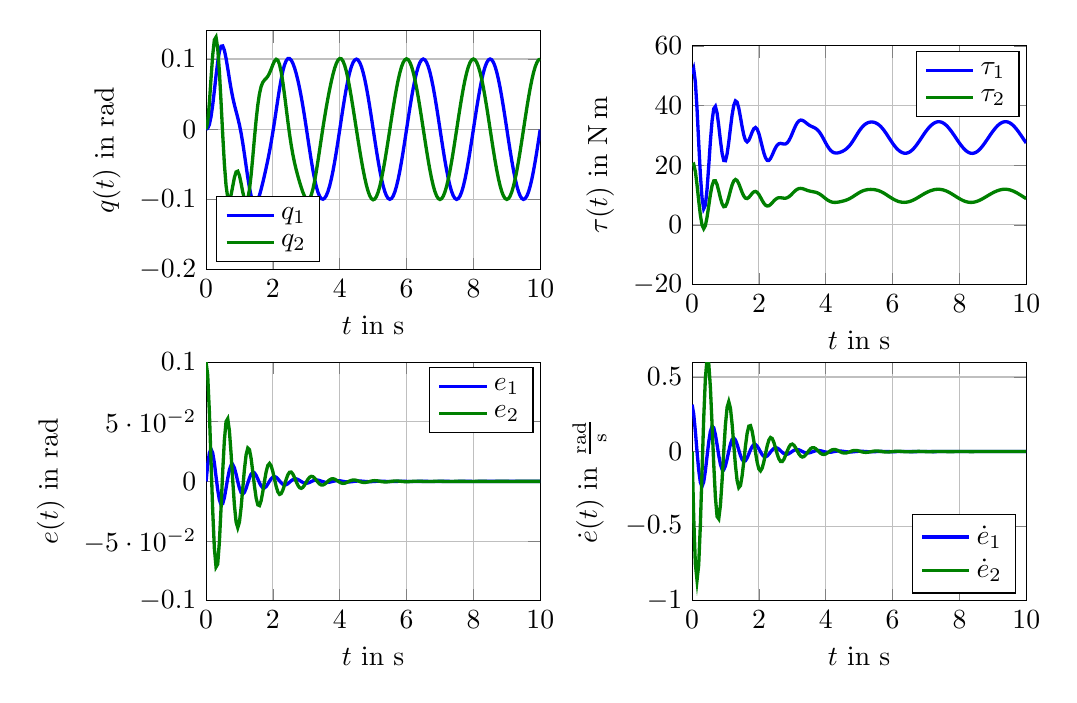
\begin{tikzpicture}

\begin{axis}[%
width=0.35\textwidth,
height=0.25\textwidth,
scale only axis,
xmin=0,
xmax=10,
xlabel={$t$ in $\mathrm{s}$},
xmajorgrids,
ymin=-0.2,
ymax=0.14,
ylabel={$q(t)$ in $\mathrm{rad}$},
ymajorgrids,
name=plot1,
legend style={at={(0.03,0.03)},anchor=south west,draw=black,fill=white,legend cell align=left}
]
\addplot [
color=blue,
solid,
line width=1.2pt
]
table[row sep=crcr]{
0 0\\
0.0476911628767132 0.00117185989493248\\
0.0976911628767132 0.00655742708224613\\
0.147691162876713 0.0176522037473643\\
0.197691162876713 0.0342868916385828\\
0.247691162876713 0.0547538685107498\\
0.297691162876713 0.0762850736338548\\
0.347691162876713 0.0957396170379566\\
0.397691162876713 0.110322381267784\\
0.447691162876714 0.118164436516076\\
0.497691162876714 0.118644120968439\\
0.547691162876714 0.112399301968782\\
0.597691162876714 0.101057691246632\\
0.647691162876714 0.086774909019701\\
0.697691162876714 0.0717059361880253\\
0.747691162876714 0.0575388517187593\\
0.797691162876714 0.0451926826911585\\
0.847691162876714 0.0347329975587757\\
0.897691162876714 0.0255027956561174\\
0.947691162876714 0.0164161093320145\\
0.997691162876714 0.00632866052127639\\
1.04769116287671 -0.00561001235830682\\
1.0976911628767 -0.0197052057378185\\
1.1476911628767 -0.0356174507573674\\
1.19769116287669 -0.0524254053395066\\
1.24769116287669 -0.0688230317066814\\
1.29769116287668 -0.0833941336721763\\
1.34769116287668 -0.0948945611478763\\
1.39769116287667 -0.10247703492517\\
1.44769116287666 -0.105812868415809\\
1.49769116287666 -0.105092971434898\\
1.54769116287665 -0.100920035779766\\
1.59769116287665 -0.0941277198885634\\
1.64769116287664 -0.0855759377775211\\
1.69769116287664 -0.0759719390081387\\
1.74769116287663 -0.0657558230050336\\
1.79769116287663 -0.0550701494611351\\
1.84769116287662 -0.043811571979481\\
1.89769116287662 -0.0317432671217268\\
1.94769116287661 -0.0186345790834268\\
1.9976911628766 -0.00439098690899603\\
2.0476911628766 0.0108568575391716\\
2.09769116287659 0.0267238401935813\\
2.14769116287659 0.0426039807257811\\
2.19769116287658 0.0577550803352329\\
2.24769116287658 0.0714117506590965\\
2.29769116287657 0.0828995822141132\\
2.34769116287657 0.0917253777886937\\
2.39769116287656 0.0976261389301275\\
2.44769116287655 0.100570515889488\\
2.49769116287655 0.100717840621997\\
2.54769116287654 0.0983489701268369\\
2.59769116287654 0.0937880776405895\\
2.64769116287653 0.0873345048504598\\
2.69769116287653 0.0792193123157766\\
2.74769116287652 0.0695937118813615\\
2.79769116287652 0.0585481614924438\\
2.84769116287651 0.0461536049760082\\
2.89769116287651 0.0325117488158687\\
2.9476911628765 0.0178002025886046\\
2.99769116287649 0.00230068740216\\
3.04769116287649 -0.0135965401065272\\
3.09769116287648 -0.0294127847159783\\
3.14769116287648 -0.0446205129886941\\
3.19769116287647 -0.0586933529286241\\
3.24769116287647 -0.0711557635435755\\
3.29769116287646 -0.081622627178627\\
3.34769116287646 -0.089822133091697\\
3.39769116287645 -0.0955996447124325\\
3.44769116287644 -0.0989046578463231\\
3.49769116287644 -0.0997664312907757\\
3.54769116287643 -0.0982656914919106\\
3.59769116287643 -0.0945097193996139\\
3.64769116287642 -0.0886163319395368\\
3.69769116287642 -0.0807093605878925\\
3.74769116287641 -0.0709249971353963\\
3.79769116287641 -0.0594256132054338\\
3.8476911628764 -0.0464159718848651\\
3.8976911628764 -0.0321564345863252\\
3.94769116287639 -0.0169687727276753\\
3.99769116287638 -0.00123216681366604\\
4.0476911628764 0.0146306325015835\\
4.09769116287642 0.0301747899320173\\
4.14769116287643 0.0449587824204366\\
4.19769116287645 0.0585693962939539\\
4.24769116287647 0.0706424483733721\\
4.29769116287648 0.0808766041675779\\
4.3476911628765 0.0890393647165325\\
4.39769116287652 0.0949660065307203\\
4.44769116287653 0.0985535908747439\\
4.49769116287655 0.0997528411212794\\
4.54769116287657 0.0985606293615082\\
4.59769116287658 0.0950151068176576\\
4.6476911628766 0.0891943907553605\\
4.69769116287662 0.081218492120647\\
4.74769116287663 0.0712531371062421\\
4.79769116287665 0.0595135312486993\\
4.84769116287667 0.0462660439381591\\
4.89769116287668 0.0318262267011825\\
4.9476911628767 0.0165523766060006\\
4.99769116287672 0.000834801318177641\\
5.04769116287673 -0.014918195390584\\
5.09769116287675 -0.0302959994597762\\
5.14769116287677 -0.0449012283513484\\
5.19769116287678 -0.0583634998714761\\
5.2476911628768 -0.0703502984593544\\
5.29769116287682 -0.0805744774614679\\
5.34769116287683 -0.0887986037429132\\
5.39769116287685 -0.0948368669502254\\
5.44769116287687 -0.0985555389973002\\
5.49769116287688 -0.0998729484056209\\
5.5476911628769 -0.0987596674396199\\
5.59769116287692 -0.0952391901503442\\
5.64769116287693 -0.0893889263463632\\
5.69769116287695 -0.0813409665717885\\
5.74769116287697 -0.0712818723736004\\
5.79769116287698 -0.0594507527074376\\
5.847691162877 -0.0461350871768251\\
5.89769116287702 -0.0316640916137139\\
5.94769116287703 -0.0163998063816397\\
5.99769116287705 -0.000726433382439197\\
6.04769116287707 0.014961318578919\\
6.09769116287708 0.0302700394012031\\
6.1476911628771 0.0448188076721527\\
6.19769116287712 0.0582491948694835\\
6.24769116287713 0.0702337754807559\\
6.29769116287715 0.0804830964971692\\
6.34769116287717 0.0887512632480978\\
6.39769116287718 0.0948404058769597\\
6.4476911628772 0.0986042909868279\\
6.49769116287722 0.099951252042321\\
6.54769116287723 0.0988464663910651\\
6.59769116287725 0.0953134525186415\\
6.64769116287727 0.0894345426069774\\
6.69769116287728 0.0813500345382189\\
6.7476911628773 0.0712557573121863\\
6.79769116287732 0.0593988873264751\\
6.84769116287733 0.0460720061623347\\
6.89769116287735 0.0316055596464171\\
6.94769116287737 0.0163590280429053\\
6.99769116287739 0.000711220218048735\\
7.0476911628774 -0.0149498548712998\\
7.09769116287742 -0.0302371084138475\\
7.14769116287744 -0.0447741249436472\\
7.19769116287745 -0.0582042894444185\\
7.24769116287747 -0.0701991311565872\\
7.29769116287749 -0.0804658086516356\\
7.3476911628775 -0.0887537081236979\\
7.39769116287752 -0.0948601360205399\\
7.44769116287754 -0.0986350645219344\\
7.49769116287755 -0.0999848480636331\\
7.54769116287757 -0.0988747886991126\\
7.59769116287759 -0.0953304041022282\\
7.6476911628776 -0.0894372559501315\\
7.69769116287762 -0.0813392324013874\\
7.74769116287764 -0.0712352426748549\\
7.79769116287765 -0.0593743642017532\\
7.84769116287767 -0.0460495697002319\\
7.89769116287769 -0.0315902387910202\\
7.9476911628777 -0.0163537152915167\\
7.99769116287772 -0.000716201002231182\\
8.04769116287769 0.0149367205938877\\
8.09769116287767 0.030219656732332\\
8.14769116287764 0.0447568328156469\\
8.19769116287761 0.0581911706140087\\
8.24769116287758 0.0701928450646133\\
8.29769116287756 0.0804671696862493\\
8.34769116287753 0.0887616714544062\\
8.3976911628775 0.0948722179634054\\
8.44769116287747 0.0986480581430871\\
8.49769116287744 0.0999956391955574\\
8.54769116287742 0.0988810726888984\\
8.59769116287739 0.095331145741776\\
8.64769116287736 0.0894328098677191\\
8.69769116287733 0.0813311281756986\\
8.74769116287731 0.0712257166440603\\
8.79769116287728 0.0593657711575367\\
8.84769116287725 0.0460438229678111\\
8.89769116287722 0.0315884064507547\\
8.9476911628772 0.0163558517604057\\
8.99769116287717 0.000721430818009667\\
9.04769116287714 -0.0149299103073291\\
9.09769116287711 -0.0302130031189634\\
9.14769116287708 -0.0447518712047339\\
9.19769116287706 -0.0581888960058763\\
9.24769116287703 -0.0701935317226224\\
9.297691162877 -0.0804703758228168\\
9.34769116287697 -0.088766410305238\\
9.39769116287695 -0.0948772395570794\\
9.44769116287692 -0.0986521655818727\\
9.49769116287689 -0.0999979624723893\\
9.54769116287686 -0.0988812402843077\\
9.59769116287683 -0.0953293237475903\\
9.64769116287681 -0.0894296121285147\\
9.69769116287678 -0.0813274306586137\\
9.74769116287675 -0.071222428401194\\
9.79769116287672 -0.0593636193756262\\
9.8476911628767 -0.0460432008463119\\
9.89769116287667 -0.0315893133726021\\
9.94769116287664 -0.016357930912382\\
9.99769116287661 -0.000724086221916131\\
};
\addlegendentry{$q_1$};

\addplot [
color=green!50!black,
solid,
line width=1.2pt
]
table[row sep=crcr]{
0 0\\
0.0476911628767132 0.0096928758824843\\
0.0976911628767132 0.0366802910311679\\
0.147691162876713 0.0720784652163575\\
0.197691162876713 0.105386834630719\\
0.247691162876713 0.127145999523954\\
0.297691162876713 0.131089336220913\\
0.347691162876713 0.115355771788105\\
0.397691162876713 0.0825691046716921\\
0.447691162876714 0.0388716533817807\\
0.497691162876714 -0.00776487288737662\\
0.547691162876714 -0.0494908380276979\\
0.597691162876714 -0.0803148064358274\\
0.647691162876714 -0.0972423206190483\\
0.697691162876714 -0.100610826690812\\
0.747691162876714 -0.0936211191948797\\
0.797691162876714 -0.0812527302279281\\
0.847691162876714 -0.0688762281689116\\
0.897691162876714 -0.0609160262649143\\
0.947691162876714 -0.0598716479954418\\
0.997691162876714 -0.0658923086117955\\
1.04769116287671 -0.0769519227507249\\
1.0976911628767 -0.089526966616253\\
1.1476911628767 -0.0995714350349789\\
1.19769116287669 -0.103533180601278\\
1.24769116287669 -0.0991703087142256\\
1.29769116287668 -0.0859955614137448\\
1.34769116287668 -0.065279403098442\\
1.39769116287667 -0.0396516921847393\\
1.44769116287666 -0.0124313463621598\\
1.49769116287666 0.0131356981715539\\
1.54769116287665 0.0345458485030111\\
1.59769116287665 0.0504693705808854\\
1.64769116287664 0.0608681513442289\\
1.69769116287664 0.0668041057856083\\
1.74769116287663 0.0700142173581391\\
1.79769116287663 0.0723752257522676\\
1.84769116287662 0.0753948211453603\\
1.89769116287662 0.0798468042548831\\
1.94769116287661 0.0856227154891271\\
1.9976911628766 0.0918148363822626\\
2.0476911628766 0.0969898524535032\\
2.09769116287659 0.0995716143628435\\
2.14769116287659 0.0982334647121398\\
2.19769116287658 0.0922075279232913\\
2.24769116287658 0.0814462138568021\\
2.29769116287657 0.0666114890678613\\
2.34769116287657 0.0489096549052315\\
2.39769116287656 0.0298234377416862\\
2.44769116287655 0.0108119849507519\\
2.49769116287655 -0.0069500477438348\\
2.54769116287654 -0.0227391384156427\\
2.59769116287654 -0.03632738445014\\
2.64769116287653 -0.0479080897832286\\
2.69769116287653 -0.0579330845395825\\
2.74769116287652 -0.0669099898269644\\
2.79769116287652 -0.0752122691554691\\
2.84769116287651 -0.082946740367488\\
2.89769116287651 -0.0899053827318181\\
2.9476911628765 -0.0956058446787801\\
2.99769116287649 -0.0994037069391053\\
3.04769116287649 -0.100644162037783\\
3.09769116287648 -0.0988143610355842\\
3.14769116287648 -0.0936608981621542\\
3.19769116287647 -0.0852480946602029\\
3.24769116287647 -0.0739485465953538\\
3.29769116287646 -0.0603737040794507\\
3.34769116287646 -0.0452652125762747\\
3.39769116287645 -0.0293746748172109\\
3.44769116287644 -0.0133593505014279\\
3.49769116287644 0.00228518884886557\\
3.54769116287643 0.017245167141233\\
3.59769116287643 0.0313632526583312\\
3.64769116287642 0.0445799796042785\\
3.69769116287642 0.0568607309989247\\
3.74769116287641 0.0681285791010242\\
3.79769116287641 0.0782198676515962\\
3.8476911628764 0.0868723549425584\\
3.8976911628764 0.0937470157914498\\
3.94769116287639 0.0984764183285315\\
3.99769116287638 0.100726808987077\\
4.0476911628764 0.100258781677022\\
4.09769116287642 0.0969728724066144\\
4.14769116287643 0.0909309204168042\\
4.19769116287645 0.0823502417076387\\
4.24769116287647 0.071573970445806\\
4.29769116287648 0.0590258656213784\\
4.3476911628765 0.0451604403858582\\
4.39769116287652 0.0304190865816668\\
4.44769116287653 0.0152002473165254\\
4.49769116287655 -0.000152516798551499\\
4.54769116287657 -0.0153453814792595\\
4.59769116287658 -0.0301168261867478\\
4.6476911628766 -0.0442151443793406\\
4.69769116287662 -0.057378596212236\\
4.74769116287663 -0.0693244862449832\\
4.79769116287665 -0.0797506557011363\\
4.84769116287667 -0.0883494943878756\\
4.89769116287668 -0.0948314502899699\\
4.9476911628767 -0.0989528541279281\\
4.99769116287672 -0.100542099080834\\
5.04769116287673 -0.0995188783290955\\
5.09769116287675 -0.0959030008235646\\
5.14769116287677 -0.089811752753976\\
5.19769116287678 -0.081447226225893\\
5.2476911628768 -0.0710769329338813\\
5.29769116287682 -0.0590119779343133\\
5.34769116287683 -0.0455869604588908\\
5.39769116287685 -0.0311447283078597\\
5.44769116287687 -0.0160274767857102\\
5.49769116287688 -0.00057389520836444\\
5.5476911628769 0.0148794410751795\\
5.59769116287692 0.0299951306246222\\
5.64769116287693 0.0444332885243238\\
5.69769116287695 0.0578534141984614\\
5.74769116287697 0.0699209235319904\\
5.79769116287698 0.0803181735623998\\
5.847691162877 0.0887586177457811\\
5.89769116287702 0.0950019299026378\\
5.94769116287703 0.0988676795634189\\
5.99769116287705 0.100245444043372\\
6.04769116287707 0.0990999860987429\\
6.09769116287708 0.0954711023481871\\
6.1476911628771 0.0894687146335235\\
6.19769116287712 0.081264517419311\\
6.24769116287713 0.0710818657810146\\
6.29769116287715 0.0591855466569456\\
6.34769116287717 0.0458726771068411\\
6.39769116287718 0.0314653509000632\\
6.4476911628772 0.0163049810814876\\
6.49769116287722 0.000747728173607642\\
6.54769116287723 -0.0148399155002573\\
6.59769116287725 -0.0300863405449861\\
6.64769116287727 -0.0446215416304097\\
6.69769116287728 -0.0580856141413796\\
6.7476911628773 -0.0701387874868379\\
6.79769116287732 -0.0804723052189896\\
6.84769116287733 -0.0888191705903486\\
6.89769116287735 -0.0949637008078454\\
6.94769116287737 -0.0987489759471504\\
6.99769116287739 -0.100081581062531\\
7.0476911628774 -0.0989334399996503\\
7.09769116287742 -0.0953409323729921\\
7.14769116287744 -0.0894017876999676\\
7.19769116287745 -0.0812704085967437\\
7.24769116287747 -0.0711522729127194\\
7.29769116287749 -0.059297925939278\\
7.3476911628775 -0.045996850887152\\
7.39769116287752 -0.0315712652853036\\
7.44769116287754 -0.0163696964777512\\
7.49769116287755 -0.000760087013053258\\
7.54769116287757 0.0148778103433145\\
7.59769116287759 0.0301608776048922\\
7.6476911628776 0.0447118674001238\\
7.69769116287762 0.0581691809442641\\
7.74769116287764 0.0701967681266185\\
7.79769116287765 0.0804936255154617\\
7.84769116287767 0.0888023517778086\\
7.89769116287769 0.0949162909512592\\
7.9476911628777 0.0986849322868427\\
7.99769116287772 0.10001740817509\\
8.04769116287769 0.0988841019524292\\
8.09769116287767 0.0953165128148744\\
8.14769116287764 0.0894056048850133\\
8.19769116287761 0.0812988860699599\\
8.24769116287758 0.0711964289137992\\
8.29769116287756 0.0593459804637611\\
8.34769116287753 0.0460372366214325\\
8.3976911628775 0.0315953024580188\\
8.44769116287747 0.0163733403911464\\
8.49769116287744 0.000744429339653172\\
8.54769116287742 -0.0149072847019349\\
8.59769116287739 -0.0301959865273475\\
8.64769116287736 -0.0447438945884931\\
8.69769116287733 -0.0581909575854466\\
8.74769116287731 -0.0702041959058269\\
8.79769116287728 -0.0804863392942586\\
8.84769116287725 -0.0887834494097442\\
8.89769116287722 -0.0948912819595008\\
8.9476911628772 -0.0986602246886147\\
8.99769116287717 -0.0999987299618738\\
9.04769116287714 -0.0988752312267441\\
9.09769116287711 -0.0953185830790634\\
9.14769116287708 -0.0894170926112381\\
9.19769116287706 -0.0813162185198606\\
9.24769116287703 -0.0712150115661346\\
9.297691162877 -0.0593613647366256\\
9.34769116287697 -0.0460461424683122\\
9.39769116287695 -0.0315962713915629\\
9.44769116287692 -0.0163669019547862\\
9.49769116287689 -0.000732788542072799\\
9.54769116287686 0.014920920577795\\
9.59769116287683 0.0302082505745832\\
9.64769116287681 0.0447520599288591\\
9.69769116287678 0.0581935118034095\\
9.74769116287675 0.0702010778578877\\
9.79769116287672 0.0804788152481056\\
9.8476911628767 0.0887736916941292\\
9.89769116287667 0.0948817766058962\\
9.94769116287664 0.0986531623529935\\
9.99769116287661 0.0999955236280759\\
};
\addlegendentry{$q_2$};

\end{axis}

\begin{axis}[%
width=0.35\textwidth,
height=0.25\textwidth,
scale only axis,
xmin=0,
xmax=10,
xlabel={$t$ in $\mathrm{s}$},
xmajorgrids,
ymin=-0.1,
ymax=0.1,
ylabel={$e(t)$ in $\mathrm{rad}$},
ymajorgrids,
name=plot3,
at=(plot1.below south west),
anchor=above north west,
legend style={draw=black,fill=white,legend cell align=left}
]
\addplot [
color=blue,
solid,
line width=1.2pt
]
table[row sep=crcr]{
0 0\\
0.0476911628767132 0.0137547689711745\\
0.0976911628767132 0.0236536237228357\\
0.147691162876713 0.0270993726611421\\
0.197691162876713 0.0239032780402037\\
0.247691162876713 0.0154420593387241\\
0.297691162876713 0.00418815567572452\\
0.347691162876713 -0.00697060424920974\\
0.397691162876713 -0.0154433727021912\\
0.447691162876714 -0.0195116682498993\\
0.497691162876714 -0.0186467515661574\\
0.547691162876714 -0.0135195985373215\\
0.597691162876714 -0.00573040024739728\\
0.647691162876714 0.00265269526976655\\
0.697691162876714 0.00961997698086578\\
0.747691162876714 0.0136828564421058\\
0.797691162876714 0.0141711056354624\\
0.847691162876714 0.0113111374478816\\
0.897691162876714 0.00608792661498934\\
0.947691162876714 -5.66682223691918e-05\\
0.997691162876714 -0.00560332430708418\\
1.04769116287671 -0.00931661650779878\\
1.0976911628767 -0.0105058450672604\\
1.1476911628767 -0.0091341256511346\\
1.19769116287669 -0.00576476433927451\\
1.24769116287669 -0.00137289614278656\\
1.29769116287668 0.00292090436260296\\
1.34769116287668 0.00612554835913487\\
1.39769116287667 0.00759802635958193\\
1.44769116287666 0.00716010014963438\\
1.49769116287666 0.00509560203261633\\
1.54769116287665 0.00204033234830323\\
1.59769116287665 -0.00119957111067739\\
1.64769116287664 -0.00385166651195652\\
1.69769116287664 -0.00535397416076643\\
1.74769116287663 -0.00546588515584959\\
1.79769116287663 -0.00429363886550795\\
1.84769116287662 -0.00223256302720235\\
1.89769116287662 0.000152544850590582\\
1.94769116287661 0.00227513797374906\\
1.9976911628766 0.00366565069476931\\
2.0476911628766 0.0040697713268998\\
2.09769116287659 0.00348721061146464\\
2.14769116287659 0.00214759568269002\\
2.19769116287658 0.000435089343520184\\
2.24769116287658 -0.0012158228096531\\
2.29769116287657 -0.00242635290456042\\
2.34769116287657 -0.00295636499996818\\
2.39769116287656 -0.00274713036455014\\
2.44769116287655 -0.00191774762331863\\
2.49769116287655 -0.000720471219716107\\
2.54769116287654 0.000530733304631131\\
2.59769116287654 0.00153921335866181\\
2.64769116287653 0.00209309943903331\\
2.69769116287653 0.00210660085314864\\
2.74769116287652 0.00162799627954595\\
2.79769116287652 0.000815626834227041\\
2.84769116287651 -0.000109469969294139\\
2.89769116287651 -0.000921026544699645\\
2.9476911628765 -0.00144076147889281\\
2.99769116287649 -0.0015753511878988\\
3.04769116287649 -0.00133008875950997\\
3.09769116287648 -0.00079826608903464\\
3.14769116287648 -0.000131063419746121\\
3.19769116287647 0.000503183249899113\\
3.24769116287647 0.000959835694156849\\
3.29769116287646 0.00114939786909471\\
3.34769116287646 0.00105312030298746\\
3.39769116287645 0.000720636146866058\\
3.44769116287644 0.000251889580159786\\
3.49769116287644 -0.000230938111505402\\
3.54769116287643 -0.00061401193956262\\
3.59769116287643 -0.000817571599647779\\
3.64769116287642 -0.000811272349971734\\
3.69769116287642 -0.000616552581052865\\
3.74769116287641 -0.000296711025535468\\
3.79769116287641 6.18248787351144e-05\\
3.8476911628764 0.000371836878120445\\
3.8976911628764 0.000565712315123319\\
3.94769116287639 0.00060933161792933\\
3.99769116287638 0.000506830599370189\\
4.0476911628764 0.000295996364426069\\
4.09769116287642 3.62608729756186e-05\\
4.14769116287643 -0.000207206012008992\\
4.19769116287645 -0.000379226615234707\\
4.24769116287647 -0.000446520523953386\\
4.29769116287648 -0.000403374858041566\\
4.3476911628765 -0.000270351927816603\\
4.39769116287652 -8.69979651472591e-05\\
4.44769116287653 9.91773914239963e-05\\
4.49769116287655 0.000244528281001952\\
4.54769116287657 0.000319074069958777\\
4.59769116287658 0.000312184181589306\\
4.6476911628766 0.000233213534123061\\
4.69769116287662 0.000107421048261822\\
4.74769116287663 -3.14289453593186e-05\\
4.79769116287665 -0.000149742922062379\\
4.84769116287667 -0.000221908931488754\\
4.89769116287668 -0.000235504430066667\\
4.9476911628767 -0.000192935496351049\\
4.99769116287672 -0.000109465103986405\\
5.04769116287673 -8.4334755293819e-06\\
5.09769116287675 8.49486546833679e-05\\
5.14769116287677 0.000149651942826894\\
5.19769116287678 0.000173330192671697\\
5.2476911628768 0.000154370609860927\\
5.29769116287682 0.000101248151869085\\
5.34769116287683 2.95909541489642e-05\\
5.39769116287685 -4.21416153808529e-05\\
5.44769116287687 -9.72292688847798e-05\\
5.49769116287688 -0.000124420996661198\\
5.5476911628769 -0.000120035991831399\\
5.59769116287692 -8.81008488710089e-05\\
5.64769116287693 -3.86779430734258e-05\\
5.69769116287695 1.50534029407234e-05\\
5.74769116287697 6.01642127911611e-05\\
5.79769116287698 8.6964380885117e-05\\
5.847691162877 9.0952170247717e-05\\
5.89769116287702 7.33693426976934e-05\\
5.94769116287703 4.03652720935635e-05\\
5.99769116287705 1.09716835292896e-06\\
6.04769116287707 -3.46897127019817e-05\\
6.09769116287708 -5.89885960100185e-05\\
6.1476911628771 -6.72312635375122e-05\\
6.19769116287712 -5.90251905936492e-05\\
6.24769116287713 -3.78476311878317e-05\\
6.29769116287715 -9.86718750824178e-06\\
6.34769116287717 1.77495407147066e-05\\
6.39769116287718 3.86026886796537e-05\\
6.4476911628772 4.84772793742649e-05\\
6.49769116287722 4.61173599617948e-05\\
6.54769116287723 3.32370403705456e-05\\
6.59769116287725 1.38384805420805e-05\\
6.64769116287727 -6.93831758760699e-06\\
6.69769116287728 -2.4121369432098e-05\\
6.7476911628773 -3.40491514506797e-05\\
6.79769116287732 -3.50990000070051e-05\\
6.84769116287733 -2.78711558506645e-05\\
6.89769116287735 -1.48373755002942e-05\\
6.94769116287737 4.13066537172796e-07\\
6.99769116287739 1.41159959327432e-05\\
7.0476911628774 2.32260049788241e-05\\
7.09769116287742 2.60576085545708e-05\\
7.14769116287744 2.25485349379523e-05\\
7.19769116287745 1.41197654434169e-05\\
7.24769116287747 3.20330694425497e-06\\
7.29769116287749 -7.4206580875924e-06\\
7.3476911628775 -1.53046651630712e-05\\
7.39769116287752 -1.88725451325811e-05\\
7.44769116287754 -1.77037442849887e-05\\
7.49769116287755 -1.25213386504702e-05\\
7.54769116287757 -4.91473230732065e-06\\
7.59769116287759 3.11310307626878e-06\\
7.6476911628776 9.65166078878421e-06\\
7.69769116287762 1.33192326615961e-05\\
7.74769116287764 1.35345141930726e-05\\
7.79769116287765 1.05758753693799e-05\\
7.84769116287767 5.43469384094164e-06\\
7.89769116287769 -4.83479797142028e-07\\
7.9476911628777 -5.72581782231837e-06\\
7.99769116287772 -9.13521164550566e-06\\
8.04769116287769 -1.00917274761698e-05\\
8.09769116287767 -8.60592696489554e-06\\
8.14769116287764 -5.2564068807881e-06\\
8.19769116287761 -1.0009349928064e-06\\
8.24769116287758 3.08278505514736e-06\\
8.29769116287756 6.05962348698696e-06\\
8.34769116287753 7.34133445828844e-06\\
8.3976911628775 6.79060226520256e-06\\
8.44769116287747 4.7101231289981e-06\\
8.49769116287744 1.7302067259195e-06\\
8.54769116287742 -1.36925747129535e-06\\
8.59769116287739 -3.85474260551633e-06\\
8.64769116287736 -5.20557834256252e-06\\
8.69769116287733 -5.21500692074461e-06\\
8.74769116287731 -4.00848332564319e-06\\
8.79769116287728 -1.98283105851821e-06\\
8.84769116287725 3.12038696610728e-07\\
8.89769116287722 2.31582020056992e-06\\
8.9476911628772 3.58934909075806e-06\\
8.99769116287717 3.90539604004615e-06\\
9.04769116287714 3.28144108968816e-06\\
9.09769116287711 1.95231376223445e-06\\
9.14769116287708 2.94796123484486e-07\\
9.19769116287706 -1.27367299796594e-06\\
9.24769116287703 -2.39612692209956e-06\\
9.297691162877 -2.85348681608455e-06\\
9.34769116287697 -2.60248354640169e-06\\
9.39769116287695 -1.76900853622597e-06\\
9.44769116287692 -6.0268431488486e-07\\
9.49769116287689 5.93070107177129e-07\\
9.54769116287686 1.53685285458893e-06\\
9.59769116287683 2.0327483671867e-06\\
9.64769116287681 2.00783906019464e-06\\
9.69769116287678 1.51748973452326e-06\\
9.74769116287675 7.20240337134803e-07\\
9.79769116287672 -1.68950992064654e-07\\
9.8476911628767 -9.34160350310465e-07\\
9.89769116287667 -1.40889851830972e-06\\
9.94769116287664 -1.51019728619403e-06\\
9.99769116287661 -1.24999230767205e-06\\
};
\addlegendentry{$e_1$};

\addplot [
color=green!50!black,
solid,
line width=1.2pt
]
table[row sep=crcr]{
0 0.1\\
0.0476911628767132 0.0891868275489758\\
0.0976911628767132 0.0586469999680668\\
0.147691162876713 0.0173491390731101\\
0.197691162876713 -0.0240609214618273\\
0.247691162876713 -0.0559242913630885\\
0.297691162876713 -0.0717255478942925\\
0.347691162876713 -0.0693116367814479\\
0.397691162876713 -0.0509783824005852\\
0.447691162876714 -0.0225122122721352\\
0.497691162876714 0.00849020910156893\\
0.547691162876714 0.0345642091615908\\
0.597691162876714 0.0501037556307454\\
0.647691162876714 0.0524907442105418\\
0.697691162876714 0.0424206570120258\\
0.747691162876714 0.0234251913454056\\
0.797691162876714 0.00077950091834865\\
0.847691162876714 -0.0198927846198353\\
0.897691162876714 -0.0339629823006783\\
0.947691162876714 -0.0387811202707353\\
0.997691162876714 -0.0341050607904862\\
1.04769116287671 -0.0219277806807354\\
1.0976911628767 -0.00580032438298261\\
1.1476911628767 0.010143830745509\\
1.19769116287669 0.0222072674323833\\
1.24769116287669 0.0279486005533546\\
1.29769116287668 0.0266317730871157\\
1.34769116287668 0.0192352680917741\\
1.39769116287667 0.00806096991361949\\
1.44769116287666 -0.00392809474750082\\
1.49769116287666 -0.0138610343857633\\
1.54769116287665 -0.0196192196369226\\
1.59769116287665 -0.020258319775823\\
1.64769116287664 -0.0161165749357424\\
1.69769116287664 -0.00861393610684121\\
1.74769116287663 0.000181710491316503\\
1.79769116287663 0.00809800355729542\\
1.84769116287662 0.0133741916433732\\
1.89769116287662 0.0150322043106997\\
1.94769116287661 0.0130300527770447\\
1.9976911628766 0.00818253302001888\\
2.0476911628766 0.00188985097796228\\
2.09769116287659 -0.00424432336359751\\
2.14769116287659 -0.00880586042265448\\
2.19769116287658 -0.0108816147543761\\
2.24769116287658 -0.0102245056959068\\
2.29769116287657 -0.00724770074120438\\
2.34769116287657 -0.00286551989853287\\
2.39769116287656 0.00176728452946638\\
2.44769116287655 0.00554745615894283\\
2.49769116287655 0.00767538395807876\\
2.54769116287654 0.00781250954958836\\
2.59769116287654 0.00611633364511061\\
2.64769116287653 0.00315651337477302\\
2.69769116287653 -0.000257085139156434\\
2.74769116287652 -0.00328593802246671\\
2.79769116287652 -0.00526096015407347\\
2.84769116287651 -0.00582227242122947\\
2.89769116287651 -0.00497362583375376\\
2.9476911628765 -0.00304692358738604\\
2.99769116287649 -0.000593662463175895\\
3.04769116287649 0.00176445860631239\\
3.09769116287648 0.00348707003632769\\
3.14769116287648 0.00423329387265346\\
3.19769116287647 0.00392218149126765\\
3.24769116287647 0.00272683843443414\\
3.29769116287646 0.00100991575276586\\
3.34769116287646 -0.00077892243045459\\
3.39769116287645 -0.00221604745397446\\
3.44769116287644 -0.00300009060830101\\
3.49769116287644 -0.00301052506314418\\
3.54769116287643 -0.00231853827521293\\
3.59769116287643 -0.00115220185333474\\
3.64769116287642 0.000171596804146107\\
3.69769116287642 0.00132943867978609\\
3.74769116287641 0.00206734874838224\\
3.79769116287641 0.00225336165792579\\
3.8476911628764 0.00189665784614328\\
3.8976911628764 0.00113199277411112\\
3.94769116287639 0.000176349937628981\\
3.99769116287638 -0.000729439584796543\\
4.0476911628764 -0.00137907824554764\\
4.09769116287642 -0.00164558140735152\\
4.14769116287643 -0.00150331612729711\\
4.19769116287645 -0.00102432853869927\\
4.24769116287647 -0.000352262284886301\\
4.29769116287648 0.000337922705300815\\
4.3476911628765 0.00088369462085882\\
4.39769116287652 0.00117163568949884\\
4.44769116287653 0.00115919379317588\\
4.49769116287655 0.00087785301279513\\
4.54769116287657 0.000418752613197942\\
4.59769116287658 -9.42246182952002e-05\\
4.6476911628766 -0.000536432029134074\\
4.69769116287662 -0.000811573466525911\\
4.74769116287663 -0.000871441604472875\\
4.79769116287665 -0.000722573608431296\\
4.84769116287667 -0.000419518400864516\\
4.89769116287668 -4.75582756197385e-05\\
4.9476911628767 0.000300085861751606\\
4.99769116287672 0.000544729678552069\\
5.04769116287673 0.000639174897636319\\
5.09769116287675 0.000575709824333456\\
5.14769116287677 0.000384148464515885\\
5.19769116287678 0.000121313057014544\\
5.2476911628768 -0.000144775226964697\\
5.29769116287682 -0.000351810392281333\\
5.34769116287683 -0.000457174547733044\\
5.39769116287685 -0.00044599396320617\\
5.44769116287687 -0.000331964323887633\\
5.49769116287688 -0.000151441005774223\\
5.5476911628769 4.718779098563e-05\\
5.59769116287692 0.00021592018052086\\
5.64769116287693 0.000318287884244602\\
5.69769116287695 0.000336755480385836\\
5.74769116287697 0.000275004317540323\\
5.79769116287698 0.000155055747230112\\
5.847691162877 1.03950430072886e-05\\
5.89769116287702 -0.000122921337015011\\
5.94769116287703 -0.000214911297225326\\
5.99769116287705 -0.000248074641089321\\
6.04769116287707 -0.000220282667299412\\
6.09769116287708 -0.000143811348987694\\
6.1476911628771 -4.11103441102789e-05\\
6.19769116287712 6.13957495062128e-05\\
6.24769116287713 0.000139842379757865\\
6.29769116287715 0.000178241669564691\\
6.34769116287717 0.000171457899689718\\
6.39769116287718 0.000125371370903272\\
6.4476911628772 5.44600280068634e-05\\
6.49769116287722 -2.23919595737688e-05\\
6.54769116287723 -8.67133660114629e-05\\
6.59769116287725 -0.000124710260256931\\
6.64769116287727 -0.000130034778252332\\
6.69769116287728 -0.000104555537552911\\
6.7476911628773 -5.71403627674938e-05\\
6.79769116287732 -9.24090702486557e-07\\
6.84769116287733 5.01578015117549e-05\\
6.89769116287735 8.46922421895435e-05\\
6.94769116287737 9.62076809395834e-05\\
6.99769116287739 8.42116602473714e-05\\
7.0476911628774 5.37365682224816e-05\\
7.09769116287742 1.36413738243968e-05\\
7.14769116287744 -2.58165893985418e-05\\
7.19769116287745 -5.55045720125602e-05\\
7.24769116287747 -6.94352479791854e-05\\
7.29769116287749 -6.58623871480149e-05\\
7.3476911628775 -4.72841192855344e-05\\
7.39769116287752 -1.94569855634305e-05\\
7.44769116287754 1.02553683604435e-05\\
7.49769116287755 3.47507991241754e-05\\
7.54769116287757 4.88185230582885e-05\\
7.59769116287759 5.01732004506567e-05\\
7.6476911628776 3.9709008632309e-05\\
7.69769116287762 2.09887347536672e-05\\
7.74769116287764 -8.40276938210427e-07\\
7.79769116287765 -2.03962057074292e-05\\
7.84769116287767 -3.3338988923548e-05\\
7.89769116287769 -3.72823855702142e-05\\
7.9476911628777 -3.21640206147611e-05\\
7.99769116287772 -2.00387728062773e-05\\
8.04769116287769 -4.39852101505323e-06\\
8.09769116287767 1.07781842698662e-05\\
8.14769116287764 2.19994043244021e-05\\
8.19769116287761 2.70270987672017e-05\\
8.24769116287758 2.52792468742324e-05\\
8.29769116287756 1.78078626471498e-05\\
8.34769116287753 6.89838499806639e-06\\
8.3976911628775 -4.58018714633024e-06\\
8.44769116287747 -1.38992817360108e-05\\
8.49769116287744 -1.90931256903272e-05\\
8.54769116287742 -1.93441643903981e-05\\
8.59769116287739 -1.50642779368111e-05\\
8.64769116287736 -7.68182019530994e-06\\
8.69769116287733 7.8790650166749e-07\\
8.74769116287731 8.26805622052007e-06\\
8.79769116287728 1.31099845739197e-05\\
8.84769116287725 1.44366209196695e-05\\
8.89769116287722 1.22733938577591e-05\\
8.9476911628772 7.45642241284372e-06\\
8.99769116287717 1.36055959107373e-06\\
9.04769116287714 -4.47220469598775e-06\\
9.09769116287711 -8.70792013345223e-06\\
9.14769116287708 -1.05116781774495e-05\\
9.19769116287706 -9.69464896785621e-06\\
9.24769116287703 -6.69659466101535e-06\\
9.297691162877 -2.42358992279951e-06\\
9.34769116287697 2.00746172713401e-06\\
9.39769116287695 5.54912052524309e-06\\
9.44769116287692 7.4608452040395e-06\\
9.49769116287689 7.45232793586371e-06\\
9.54769116287686 5.70828835814302e-06\\
9.59769116287683 2.80023053511602e-06\\
9.64769116287681 -4.83520326381714e-07\\
9.69769116287678 -3.34212460621069e-06\\
9.74769116287675 -5.15000840529967e-06\\
9.79769116287672 -5.58593852424683e-06\\
9.8476911628767 -4.67890538481675e-06\\
9.89769116287667 -2.76804030814592e-06\\
9.94769116287664 -3.94086820135198e-07\\
9.99769116287661 1.84577420560272e-06\\
};
\addlegendentry{$e_2$};

\end{axis}

\begin{axis}[%
width=0.35\textwidth,
height=0.25\textwidth,
scale only axis,
xmin=0,
xmax=10,
xlabel={$t$ in $\mathrm{s}$},
xmajorgrids,
ymin=-1,
ymax=0.6,
ylabel={$\dot{e}(t)$ in $\mathrm{\frac{rad}{s}}$},
ymajorgrids,
name=plot2,
at=(plot3.right of south east),
anchor=left of south west,
legend style={at={(0.97,0.03)},anchor=south east,draw=black,fill=white,legend cell align=left}
]
\addplot [
color=blue,
solid,
line width=1.2pt
]
table[row sep=crcr]{
0 0.314159265358979\\
0.0476911628767132 0.252679144282493\\
0.0976911628767132 0.136937736809088\\
0.147691162876713 0.000305182535905446\\
0.197691162876713 -0.123396170183486\\
0.247691162876713 -0.206575461580944\\
0.297691162876713 -0.233708765690863\\
0.347691162876713 -0.203807720422464\\
0.397691162876713 -0.12926656623719\\
0.447691162876714 -0.0317008641903987\\
0.497691162876714 0.0639662816732416\\
0.547691162876714 0.135625862653834\\
0.597691162876714 0.168866391101599\\
0.647691162876714 0.159599145853763\\
0.697691162876714 0.114028470467699\\
0.747691162876714 0.0462266961554484\\
0.797691162876714 -0.0258933369123749\\
0.847691162876714 -0.0851173009168817\\
0.897691162876714 -0.118873708919789\\
0.947691162876714 -0.121721146095785\\
0.997691162876714 -0.0959375598154557\\
1.04769116287671 -0.0502549216805286\\
1.0976911628767 0.00278943366449808\\
1.1476911628767 0.0501360354516001\\
1.19769116287669 0.0812957169003979\\
1.24769116287669 0.0905489104620674\\
1.29769116287668 0.077824373957303\\
1.34769116287668 0.0481782802086364\\
1.39769116287667 0.0101282311422389\\
1.44769116287666 -0.0266606739006409\\
1.49769116287666 -0.0537369278627056\\
1.54769116287665 -0.0657162609771156\\
1.59769116287665 -0.0612442463604203\\
1.64769116287664 -0.0429283803952141\\
1.69769116287664 -0.016353530070178\\
1.74769116287663 0.011502630656331\\
1.79769116287663 0.0340279062153871\\
1.84769116287662 0.0464813882689512\\
1.89769116287662 0.0469199729285942\\
1.94769116287661 0.0363848421327717\\
1.9976911628766 0.0183748842339291\\
2.0476911628766 -0.00220240070503014\\
2.09769116287659 -0.0203083563214388\\
2.14769116287659 -0.0319596177776971\\
2.19769116287658 -0.0350557796585492\\
2.24769116287658 -0.0296895863615087\\
2.29769116287657 -0.0179166175948344\\
2.34769116287657 -0.00308956626198614\\
2.39769116287656 0.0110463488236908\\
2.44769116287655 0.021263342761691\\
2.49769116287655 0.0255538722956125\\
2.54769116287654 0.0234822559978164\\
2.59769116287654 0.0161366021290458\\
2.64769116287653 0.00573028035105991\\
2.69769116287653 -0.00502085849083952\\
2.74769116287652 -0.013579071310648\\
2.79769116287652 -0.0181590474393444\\
2.84769116287651 -0.0180722683271701\\
2.89769116287651 -0.0137830532916529\\
2.9476911628765 -0.00669066980042438\\
2.99769116287649 0.00128565674274206\\
3.04769116287649 0.00820338771414331\\
3.09769116287648 0.0125514857867179\\
3.14769116287648 0.0135614117702758\\
3.19769116287647 0.0113155300591841\\
3.24769116287647 0.00664694420480405\\
3.29769116287646 0.000873948171421363\\
3.34769116287646 -0.00455329759122552\\
3.39769116287645 -0.00840319069515735\\
3.44769116287644 -0.00992884177546838\\
3.49769116287644 -0.0089959671988116\\
3.54769116287643 -0.00605587893334564\\
3.59769116287643 -0.00198460567858358\\
3.64769116287642 0.00216163195924243\\
3.69769116287642 0.00540965995193757\\
3.74769116287641 0.00708818969141775\\
3.79769116287641 0.00695549467297499\\
3.8476911628764 0.0052148525996038\\
3.8976911628764 0.00242483555284723\\
3.94769116287639 -0.000664643567310996\\
3.99769116287638 -0.00330526323954211\\
4.0476911628764 -0.00492449481375834\\
4.09769116287642 -0.00524226820616741\\
4.14769116287643 -0.00430839487756574\\
4.19769116287645 -0.00245956978166684\\
4.24769116287647 -0.000213623558568243\\
4.29769116287648 0.00186836520437508\\
4.3476911628765 0.00331691238438056\\
4.39769116287652 0.00385479800497608\\
4.44769116287653 0.00344335992179615\\
4.49769116287655 0.002268800013898\\
4.54769116287657 0.00067740199340538\\
4.59769116287658 -0.000920383731728772\\
4.6476911628766 -0.00215167799002311\\
4.69769116287662 -0.00276447533669974\\
4.74769116287663 -0.00267485665182243\\
4.79769116287665 -0.0019705460957144\\
4.84769116287667 -0.000874138063157059\\
4.89769116287668 0.000321600130880562\\
4.9476911628767 0.00132861853147176\\
4.99769116287672 0.00193024896435257\\
5.04769116287673 0.00202489411389351\\
5.09769116287675 0.00163874844543926\\
5.14769116287677 0.000907534108456176\\
5.19769116287678 3.44558234711134e-05\\
5.2476911628768 -0.000763566009058914\\
5.29769116287682 -0.00130774124747579\\
5.34769116287683 -0.00149543810877206\\
5.39769116287685 -0.00131684812752625\\
5.44769116287687 -0.000848438143374271\\
5.49769116287688 -0.000226923957865184\\
5.5476911628769 0.000388316801141021\\
5.59769116287692 0.000854534950586919\\
5.64769116287693 0.00107728676496216\\
5.69769116287695 0.00102784173729423\\
5.74769116287697 0.000743623118044545\\
5.79769116287698 0.000313193234560971\\
5.847691162877 -0.000149247349815418\\
5.89769116287702 -0.000532907454799891\\
5.94769116287703 -0.000755894296799342\\
5.99769116287705 -0.000781543806778084\\
6.04769116287707 -0.000622658983990554\\
6.09769116287708 -0.000333819485563713\\
6.1476911628771 5.31057192582063e-06\\
6.19769116287712 0.0003109308166932\\
6.24769116287713 0.000515023055185748\\
6.29769116287715 0.000579697094599957\\
6.34769116287717 0.000503151796568013\\
6.39769116287718 0.000316660400393132\\
6.4476911628772 7.41366651246869e-05\\
6.49769116287722 -0.000162581135628038\\
6.54769116287723 -0.000338892154361552\\
6.59769116287725 -0.000419465798511237\\
6.64769116287727 -0.000394639668857777\\
6.69769116287728 -0.000280228169758229\\
6.7476911628773 -0.000111413440936986\\
6.79769116287732 6.72948835158116e-05\\
6.84769116287733 0.000213317692522974\\
6.89769116287735 0.000295743276960192\\
6.94769116287737 0.000301419210673171\\
6.99769116287739 0.000236326741410442\\
7.0476911628774 0.000122366398100093\\
7.09769116287742 -9.25957721431558e-06\\
7.14769116287744 -0.00012620227736948\\
7.19769116287745 -0.000202612286465564\\
7.24769116287747 -0.00022454387875262\\
7.29769116287749 -0.000192071475361405\\
7.3476911628775 -0.000117938111391824\\
7.39769116287752 -2.33808325962453e-05\\
7.44769116287754 6.76256785005491e-05\\
7.49769116287755 0.00013421553254942\\
7.54769116287757 0.000163197378012028\\
7.59769116287759 0.000151397551774138\\
7.6476911628776 0.000105446208193194\\
7.69769116287762 3.92995895440729e-05\\
7.74769116287764 -2.97088362974929e-05\\
7.79769116287765 -8.5228320817754e-05\\
7.84769116287767 -0.000115606910440158\\
7.89769116287769 -0.000116159109108616\\
7.9476911628777 -8.95946153226523e-05\\
7.99769116287772 -4.46832382434703e-05\\
8.04769116287769 6.36509354484671e-06\\
8.09769116287767 5.10725184066918e-05\\
8.14769116287764 7.96259808206745e-05\\
8.19769116287761 8.6910005077101e-05\\
8.24769116287758 7.32515264033617e-05\\
8.29769116287756 4.38258037889494e-05\\
8.34769116287753 6.98924700792691e-06\\
8.3976911628775 -2.79702865802062e-05\\
8.44769116287747 -5.30861274993938e-05\\
8.49769116287744 -6.34432368135842e-05\\
8.54769116287742 -5.80329698616072e-05\\
8.59769116287739 -3.96163398370536e-05\\
8.64769116287736 -1.37219934067678e-05\\
8.69769116287733 1.29052949063291e-05\\
8.74769116287731 3.39918311398901e-05\\
8.79769116287728 4.51518931888217e-05\\
8.84769116287725 4.47299047209859e-05\\
8.89769116287722 3.39263635034115e-05\\
8.9476911628772 1.62463436363391e-05\\
8.99769116287717 -3.53646812656372e-06\\
9.04769116287714 -2.06127276854429e-05\\
9.09769116287711 -3.12613655686911e-05\\
9.14769116287708 -3.36130033493642e-05\\
9.19769116287706 -2.79092921728896e-05\\
9.24769116287703 -1.62457189498422e-05\\
9.297691162877 -1.90695885618486e-06\\
9.34769116287697 1.15115939478827e-05\\
9.39769116287695 2.09710932378149e-05\\
9.44769116287692 2.46443050586839e-05\\
9.49769116287689 2.22260384836761e-05\\
9.54769116287686 1.48594111120046e-05\\
9.59769116287683 4.73168702887217e-06\\
9.64769116287681 -5.5347019198293e-06\\
9.69769116287678 -1.35345734658954e-05\\
9.74769116287675 -1.76197091338315e-05\\
9.79769116287672 -1.72108413380445e-05\\
9.8476911628767 -1.28308939760791e-05\\
9.89769116287667 -5.87825794989838e-06\\
9.94769116287664 1.78233443354214e-06\\
9.99769116287661 8.29865543555686e-06\\
};
\addlegendentry{$\dot{e}_1$};

\addplot [
color=green!50!black,
solid,
line width=1.2pt
]
table[row sep=crcr]{
0 -0\\
0.0476911628767132 -0.437827894569889\\
0.0976911628767132 -0.752918227505004\\
0.147691162876713 -0.862599822742026\\
0.197691162876713 -0.760864971239671\\
0.247691162876713 -0.491536015055258\\
0.297691162876713 -0.133313135645984\\
0.347691162876713 0.221881224519822\\
0.397691162876713 0.491577820712836\\
0.447691162876714 0.621075689988132\\
0.497691162876714 0.593544536872099\\
0.547691162876714 0.430342187166533\\
0.597691162876714 0.182404305053657\\
0.647691162876714 -0.0844379129399723\\
0.697691162876714 -0.306213377787014\\
0.747691162876714 -0.435538847675591\\
0.797691162876714 -0.451080302192257\\
0.847691162876714 -0.360044687364446\\
0.897691162876714 -0.193784722791256\\
0.947691162876714 0.00180380554125664\\
0.997691162876714 0.178359352243884\\
1.04769116287671 0.296557114021593\\
1.0976911628767 0.334411434762503\\
1.1476911628767 0.290748249640209\\
1.19769116287669 0.183498148071176\\
1.24769116287669 0.0437006414953169\\
1.29769116287668 -0.0929752735213703\\
1.34769116287668 -0.194982260100978\\
1.39769116287667 -0.241852690574063\\
1.44769116287666 -0.227913066369557\\
1.49769116287666 -0.162198050304098\\
1.54769116287665 -0.0649457957566386\\
1.59769116287665 0.0381835343708417\\
1.64769116287664 0.12260235290384\\
1.69769116287664 0.17042229057444\\
1.74769116287663 0.173984528185218\\
1.79769116287663 0.136670769859425\\
1.84769116287662 0.0710646883086971\\
1.89769116287662 -0.00485565340294759\\
1.94769116287661 -0.0724198909476727\\
1.9976911628766 -0.116681285544193\\
2.0476911628766 -0.129544844786\\
2.09769116287659 -0.111001361283469\\
2.14769116287659 -0.0683600937326275\\
2.19769116287658 -0.0138493239415937\\
2.24769116287658 0.0387008420160282\\
2.29769116287657 0.0772332116892495\\
2.34769116287657 0.0941040206657934\\
2.39769116287656 0.0874438753672439\\
2.44769116287655 0.0610438027708288\\
2.49769116287655 0.0229333111947027\\
2.54769116287654 -0.0168937657790627\\
2.59769116287654 -0.0489946829007827\\
2.64769116287653 -0.0666254244209731\\
2.69769116287653 -0.0670551877800145\\
2.74769116287652 -0.0518207310449668\\
2.79769116287652 -0.0259622084771018\\
2.84769116287651 0.00348453734668472\\
2.89769116287651 0.0293171854615895\\
2.9476911628765 0.0458608622364667\\
2.99769116287649 0.0501449857319859\\
3.04769116287649 0.0423380401654267\\
3.09769116287648 0.0254095987945241\\
3.14769116287648 0.00417187822224008\\
3.19769116287647 -0.0160168203004927\\
3.24769116287647 -0.0305525190562232\\
3.29769116287646 -0.0365864704891556\\
3.34769116287646 -0.0335218603781994\\
3.39769116287645 -0.0229385609889155\\
3.44769116287644 -0.00801789435918826\\
3.49769116287644 0.00735098839884318\\
3.54769116287643 0.019544607059732\\
3.59769116287643 0.0260241122830638\\
3.64769116287642 0.0258236009383209\\
3.69769116287642 0.0196254781900898\\
3.74769116287641 0.00944460527672963\\
3.79769116287641 -0.00196794701138614\\
3.8476911628764 -0.0118359354353797\\
3.8976911628764 -0.0180071822640032\\
3.94769116287639 -0.0193956277951591\\
3.99769116287638 -0.0161329190400251\\
4.0476911628764 -0.00942185690696595\\
4.09769116287642 -0.00115421943466373\\
4.14769116287643 0.00659557221030715\\
4.19769116287645 0.0120711580736917\\
4.24769116287647 0.0142131897160979\\
4.29769116287648 0.0128398205153656\\
4.3476911628765 0.00860556913721416\\
4.39769116287652 0.00276923123819417\\
4.44769116287653 -0.00315691441795241\\
4.49769116287655 -0.00778357692981657\\
4.54769116287657 -0.0101564430896173\\
4.59769116287658 -0.00993713113126327\\
4.6476911628766 -0.00742341735047242\\
4.69769116287662 -0.00341931816464075\\
4.74769116287663 0.00100041440205303\\
4.79769116287665 0.00476646524791793\\
4.84769116287667 0.00706358067259361\\
4.89769116287668 0.00749633883304127\\
4.9476911628767 0.0061413275883755\\
4.99769116287672 0.0034843824789771\\
5.04769116287673 0.000268445863416622\\
5.09769116287675 -0.00270399966055673\\
5.14769116287677 -0.00476356928900873\\
5.19769116287678 -0.00551727139026428\\
5.2476911628768 -0.00491376912553515\\
5.29769116287682 -0.0032228287697369\\
5.34769116287683 -0.000941909324607804\\
5.39769116287685 0.00134140927971255\\
5.44769116287687 0.00309490375143362\\
5.49769116287688 0.00396044332879431\\
5.5476911628769 0.00382086428994066\\
5.59769116287692 0.00280433711780842\\
5.64769116287693 0.00123115716584227\\
5.69769116287695 -0.00047916469760656\\
5.74769116287697 -0.00191508637253601\\
5.79769116287698 -0.00276816221809692\\
5.847691162877 -0.00289509749589856\\
5.89769116287702 -0.00233541871224834\\
5.94769116287703 -0.00128486651647286\\
5.99769116287705 -3.49239532246148e-05\\
6.04769116287707 0.00110420785031249\\
6.09769116287708 0.00187766532831539\\
6.1476911628771 0.00214003758452977\\
6.19769116287712 0.00187883017001325\\
6.24769116287713 0.00120472751755174\\
6.29769116287715 0.00031408233321345\\
6.34769116287717 -0.00056498542856348\\
6.39769116287718 -0.00122876174411063\\
6.4476911628772 -0.00154307972813122\\
6.49769116287722 -0.00146796116017162\\
6.54769116287723 -0.00105796785385376\\
6.59769116287725 -0.000440492516736612\\
6.64769116287727 0.000220853508061225\\
6.69769116287728 0.000767807035751134\\
6.7476911628773 0.00108381815219136\\
6.79769116287732 0.00111723586963117\\
6.84769116287733 0.000887166444544729\\
6.89769116287735 0.000472288330559262\\
6.94769116287737 -1.31483163634816e-05\\
6.99769116287739 -0.000449326105977837\\
7.0476911628774 -0.000739306700224845\\
7.09769116287742 -0.000829439441387761\\
7.14769116287744 -0.000717742159012269\\
7.19769116287745 -0.000449446093130246\\
7.24769116287747 -0.000101964426864887\\
7.29769116287749 0.000236206883174384\\
7.3476911628775 0.000487162622678006\\
7.39769116287752 0.000600731769396901\\
7.44769116287754 0.000563527682930776\\
7.49769116287755 0.000398566588170279\\
7.54769116287757 0.000156440788242895\\
7.59769116287759 -9.90931484783908e-05\\
7.6476911628776 -0.000307221904598531\\
7.69769116287762 -0.000423964343137406\\
7.74769116287764 -0.0004308169671082\\
7.79769116287765 -0.000336640568388891\\
7.84769116287767 -0.000172991677671541\\
7.89769116287769 1.53896400328507e-05\\
7.9476911628777 0.000182258442040104\\
7.99769116287772 0.000290782818001923\\
8.04769116287769 0.000321229662144006\\
8.09769116287767 0.00027393516266036\\
8.14769116287764 0.000167316626826286\\
8.19769116287761 3.18607496302969e-05\\
8.24769116287758 -9.81280965390852e-05\\
8.29769116287756 -0.000192883806469868\\
8.34769116287753 -0.000233681933459406\\
8.3976911628775 -0.000216151582978719\\
8.44769116287747 -0.000149927875069289\\
8.49769116287744 -5.50741898912577e-05\\
8.54769116287742 4.35848196250754e-05\\
8.59769116287739 0.000122700268469611\\
8.64769116287736 0.000165698705217987\\
8.69769116287733 0.000165998825970626\\
8.74769116287731 0.000127593986991081\\
8.79769116287728 6.31154726557226e-05\\
8.84769116287725 -9.9325003748707e-06\\
8.89769116287722 -7.37148465189269e-05\\
8.9476911628772 -0.000114252529982449\\
8.99769116287717 -0.000124312616692717\\
9.04769116287714 -0.000104451513662077\\
9.09769116287711 -6.21440767874099e-05\\
9.14769116287708 -9.38365172589717e-06\\
9.19769116287706 4.05422709204573e-05\\
9.24769116287703 7.627108886335e-05\\
9.297691162877 9.08293062897303e-05\\
9.34769116287697 8.28396239311857e-05\\
9.39769116287695 5.63092902717277e-05\\
9.44769116287692 1.91840372174013e-05\\
9.49769116287689 -1.88780081678552e-05\\
9.54769116287686 -4.89195460057212e-05\\
9.59769116287683 -6.47043903442279e-05\\
9.64769116287681 -6.39115024040349e-05\\
9.69769116287678 -4.83031985463733e-05\\
9.74769116287675 -2.29259620301847e-05\\
9.79769116287672 5.37787704565917e-06\\
9.8476911628767 2.97352473816737e-05\\
9.89769116287667 4.48466325546765e-05\\
9.94769116287664 4.8071072436498e-05\\
9.99769116287661 3.97884907089702e-05\\
};
\addlegendentry{$\dot{e}_2$};

\end{axis}

\begin{axis}[%
width=0.35\textwidth,
height=0.25\textwidth,
scale only axis,
xmin=0,
xmax=10,
xlabel={$t$ in $\mathrm{s}$},
xmajorgrids,
ymin=-20,
ymax=60,
ylabel={$\tau(t)$ in $\mathrm{N\,m}$},
ymajorgrids,
at=(plot2.above north west),
anchor=below south west,
legend style={draw=black,fill=white,legend cell align=left}
]
\addplot [
color=blue,
solid,
line width=1.2pt
]
table[row sep=crcr]{
0 50.5976717733719\\
0.0476911628767132 52.2288152378228\\
0.0976911628767132 47.9326141058178\\
0.147691162876713 38.9097694625813\\
0.197691162876713 27.6356928916979\\
0.247691162876713 16.8859200581229\\
0.297691162876713 8.99297630987378\\
0.347691162876713 5.41852662903415\\
0.397691162876713 6.59148567920067\\
0.447691162876714 11.8679771152845\\
0.497691162876714 19.6787179861967\\
0.547691162876714 27.9726949715646\\
0.597691162876714 34.8220700806405\\
0.647691162876714 38.9005959697001\\
0.697691162876714 39.6924457545797\\
0.747691162876714 37.4862004718658\\
0.797691162876714 33.2316727430448\\
0.847691162876714 28.2775458164661\\
0.897691162876714 24.0224001140764\\
0.947691162876714 21.5715989045761\\
0.997691162876714 21.4967932100175\\
1.04769116287671 23.7463671272732\\
1.0976911628767 27.7127497635269\\
1.1476911628767 32.4312660909272\\
1.19769116287669 36.8470562312276\\
1.24769116287669 40.0661407671911\\
1.29769116287668 41.5316220752708\\
1.34769116287668 41.1090265479994\\
1.39769116287667 39.0825762046239\\
1.44769116287666 36.06224472865\\
1.49769116287666 32.8150100995905\\
1.54769116287665 30.0651154959238\\
1.59769116287665 28.3240349602001\\
1.64769116287664 27.7936641495643\\
1.69769116287664 28.3546695161282\\
1.74769116287663 29.6292047413105\\
1.79769116287663 31.0958503920704\\
1.84769116287662 32.2273271106011\\
1.89769116287662 32.6178697091067\\
1.94769116287661 32.0711552138876\\
1.9976911628766 30.6311128080888\\
2.0476911628766 28.552942493729\\
2.09769116287659 26.2266866143733\\
2.14769116287659 24.076908444184\\
2.19769116287658 22.4652404536231\\
2.24769116287658 21.6172920509004\\
2.29769116287657 21.5862947438356\\
2.34769116287657 22.2575176855007\\
2.39769116287656 23.3901096956251\\
2.44769116287655 24.6851118071255\\
2.49769116287655 25.86152667424\\
2.54769116287654 26.7205229125135\\
2.59769116287654 27.1827310737569\\
2.64769116287653 27.2925448892439\\
2.69769116287653 27.1923144210381\\
2.74769116287652 27.0758596451524\\
2.79769116287652 27.1342377844542\\
2.84769116287651 27.5071709017806\\
2.89769116287651 28.2510975448883\\
2.9476911628765 29.3299785129427\\
2.99769116287649 30.6289201480869\\
3.04769116287649 31.9850208855883\\
3.09769116287648 33.2262343575656\\
3.14769116287648 34.2083599151861\\
3.19769116287647 34.8421665877853\\
3.24769116287647 35.1059182046261\\
3.29769116287646 35.0420832703741\\
3.34769116287646 34.7402841829946\\
3.39769116287645 34.3113308760719\\
3.44769116287644 33.8590070044791\\
3.49769116287644 33.4564968066625\\
3.54769116287643 33.1327423558685\\
3.59769116287643 32.8711145682551\\
3.64769116287642 32.6195331381007\\
3.69769116287642 32.3084999811789\\
3.74769116287641 31.8719875204395\\
3.79769116287641 31.2659391360375\\
3.8476911628764 30.4801888978524\\
3.8976911628764 29.5415520804924\\
3.94769116287639 28.5081540322447\\
3.99769116287638 27.4571444646171\\
4.0476911628764 26.4692664795732\\
4.09769116287642 25.6140637387444\\
4.14769116287643 24.9389008741842\\
4.19769116287645 24.4637589687702\\
4.24769116287647 24.1823137151832\\
4.29769116287648 24.0684052712372\\
4.3476911628765 24.0858987803654\\
4.39769116287652 24.1993155464133\\
4.44769116287653 24.3826282832812\\
4.49769116287655 24.6242595775633\\
4.54769116287657 24.9274185233438\\
4.59769116287658 25.3061435740739\\
4.6476911628766 25.7784579294226\\
4.69769116287662 26.3586392600514\\
4.74769116287663 27.0506494511993\\
4.79769116287665 27.8443006904267\\
4.84769116287667 28.7149142733691\\
4.89769116287668 29.626298824436\\
4.9476911628767 30.5360874308654\\
4.99769116287672 31.4020172024578\\
5.04769116287673 32.1876814612712\\
5.09769116287675 32.8665826350966\\
5.14769116287677 33.4238311978295\\
5.19769116287678 33.8554214310231\\
5.2476911628768 34.1655408902384\\
5.29769116287682 34.3627466578576\\
5.34769116287683 34.4560112840517\\
5.39769116287685 34.4515829551069\\
5.44769116287687 34.3513384610826\\
5.49769116287688 34.1529006395496\\
5.5476911628769 33.8513455831724\\
5.59769116287692 33.4419492571729\\
5.64769116287693 32.9232070430171\\
5.69769116287695 32.2993471097777\\
5.74769116287697 31.5817388133836\\
5.79769116287698 30.7889104067315\\
5.847691162877 29.9452449595017\\
5.89769116287702 29.0787244134894\\
5.94769116287703 28.2182680747037\\
5.99769116287705 27.3912350998068\\
6.04769116287707 26.6215470706144\\
6.09769116287708 25.9286848170269\\
6.1476911628771 25.3275833179713\\
6.19769116287712 24.8292443457596\\
6.24769116287713 24.4417479748501\\
6.29769116287715 24.1712925382926\\
6.34769116287717 24.0229313516485\\
6.39769116287718 24.0007893383641\\
6.4476911628772 24.1077039378429\\
6.49769116287722 24.3444023752003\\
6.54769116287723 24.7084598446921\\
6.59769116287725 25.1933474871596\\
6.64769116287727 25.7878601684986\\
6.69769116287728 26.4761194049097\\
6.7476911628773 27.2382043491183\\
6.79769116287732 28.0513138688468\\
6.84769116287733 28.891245704736\\
6.89769116287735 29.7339226422721\\
6.94769116287737 30.5567091486161\\
6.99769116287739 31.3393337562592\\
7.0476911628774 32.0643377446918\\
7.09769116287742 32.7170801750017\\
7.14769116287744 33.2854179257559\\
7.19769116287745 33.7592309337453\\
7.24769116287747 34.1299715074813\\
7.29769116287749 34.3903855982763\\
7.3476911628775 34.5344934706757\\
7.39769116287752 34.5578420867797\\
7.44769116287754 34.4579685355642\\
7.49769116287755 34.2349589487921\\
7.54769116287757 33.8919623972315\\
7.59769116287759 33.435529114781\\
7.6476911628776 32.8756833671546\\
7.69769116287762 32.2257017685396\\
7.74769116287764 31.5016313950688\\
7.79769116287765 30.7216320451291\\
7.84769116287767 29.9052515392149\\
7.89769116287769 29.0727380265778\\
7.9476911628777 28.2444632689808\\
7.99769116287772 27.4404864397137\\
8.04769116287769 26.6802422403634\\
8.09769116287767 25.9823019107221\\
8.14769116287764 25.3641387847368\\
8.19769116287761 24.841834086636\\
8.24769116287758 24.4296814238011\\
8.29769116287756 24.1396838457813\\
8.34769116287753 23.9809769545461\\
8.3976911628775 23.9592461563982\\
8.44769116287747 24.0762274649965\\
8.49769116287744 24.3293836572918\\
8.54769116287742 24.7118294625147\\
8.59769116287739 25.2125439931128\\
8.64769116287736 25.8168632908188\\
8.69769116287733 26.5072007854052\\
8.74769116287731 27.2639088291813\\
8.79769116287728 28.0661777982853\\
8.84769116287725 28.8928734556732\\
8.89769116287722 29.7232361156032\\
8.9476911628772 30.5374002197557\\
8.99769116287717 31.3167316535434\\
9.04769116287714 32.0440140670496\\
9.09769116287711 32.7035382173807\\
9.14769116287708 33.2811565996123\\
9.19769116287706 33.7643593357572\\
9.24769116287703 34.1424092145597\\
9.297691162877 34.4065486784958\\
9.34769116287697 34.5502651952123\\
9.39769116287695 34.5695795281138\\
9.44769116287692 34.4633085252214\\
9.49769116287689 34.233252730753\\
9.54769116287686 33.8842693060569\\
9.59769116287683 33.4242096516183\\
9.64769116287681 32.863723909849\\
9.69769116287678 32.2159555092996\\
9.74769116287675 31.4961630379328\\
9.79769116287672 30.7213109221025\\
9.8476911628767 29.9096642546194\\
9.89769116287667 29.0804089278655\\
9.94769116287664 28.2533001500407\\
9.99769116287661 27.4483253431233\\
};
\addlegendentry{$\tau_1$};

\addplot [
color=green!50!black,
solid,
line width=1.2pt
]
table[row sep=crcr]{
0 20.079676621327\\
0.0476911628767132 20.3435260735766\\
0.0976911628767132 17.9003800320707\\
0.147691162876713 13.4351478833993\\
0.197691162876713 8.12882627984132\\
0.247691162876713 3.26616304863908\\
0.297691162876713 -0.0806283982947404\\
0.347691162876713 -1.28404251261687\\
0.397691162876713 -0.263344560433958\\
0.447691162876714 2.54481934573321\\
0.497691162876714 6.33140829071569\\
0.547691162876714 10.1426669607248\\
0.597691162876714 13.1271542701777\\
0.647691162876714 14.7277064389041\\
0.697691162876714 14.7738459389659\\
0.747691162876714 13.4735093468859\\
0.797691162876714 11.3257537565196\\
0.847691162876714 8.98012866736714\\
0.897691162876714 7.07284970567862\\
0.947691162876714 6.07737384097776\\
0.997691162876714 6.20553006564129\\
1.04769116287671 7.38052712168486\\
1.0976911628767 9.28231950775449\\
1.1476911628767 11.4470102928296\\
1.19769116287669 13.3895909493209\\
1.24769116287669 14.7169178318017\\
1.29769116287668 15.2060875161493\\
1.34769116287668 14.8366785612193\\
1.39769116287667 13.7763937566023\\
1.44769116287666 12.3268961452964\\
1.49769116287666 10.8431676924078\\
1.54769116287665 9.64608625298105\\
1.59769116287665 8.95015123594495\\
1.64769116287664 8.82334247618976\\
1.69769116287664 9.18594969043616\\
1.74769116287663 9.84455588769523\\
1.79769116287663 10.5494856084921\\
1.84769116287662 11.0599760770664\\
1.89769116287662 11.2011980151949\\
1.94769116287661 10.9006959320813\\
1.9976911628766 10.1977308742865\\
2.0476911628766 9.22578021556654\\
2.09769116287659 8.17457187978076\\
2.14769116287659 7.24227243341145\\
2.19769116287658 6.58987696422557\\
2.24769116287658 6.30822305473747\\
2.29769116287657 6.40410445813603\\
2.34769116287657 6.80698073420106\\
2.39769116287656 7.39294568412774\\
2.44769116287655 8.01883486635381\\
2.49769116287655 8.55742397693227\\
2.54769116287654 8.92513796182721\\
2.59769116287654 9.09637837914672\\
2.64769116287653 9.1025022117501\\
2.69769116287653 9.01738006177957\\
2.74769116287652 8.93436418876103\\
2.79769116287652 8.94094239420481\\
2.84769116287651 9.09724854449784\\
2.89769116287651 9.42311011176649\\
2.9476911628765 9.89585590025465\\
2.99769116287649 10.4583260286789\\
3.04769116287649 11.0341461204342\\
3.09769116287648 11.5459324399032\\
3.14769116287648 11.9319300489614\\
3.19769116287647 12.1575020735381\\
3.24769116287647 12.2194670549485\\
3.29769116287646 12.1430577841775\\
3.34769116287646 11.9728849913946\\
3.39769116287645 11.7604774265204\\
3.44769116287644 11.5515423388264\\
3.49769116287644 11.3759300299349\\
3.54769116287643 11.2424304330723\\
3.59769116287643 11.1392112833352\\
3.64769116287642 11.0392918983099\\
3.69769116287642 10.9093020009958\\
3.74769116287641 10.7191569366794\\
3.79769116287641 10.4502803968006\\
3.8476911628764 10.1005579263257\\
3.8976911628764 9.68512691043927\\
3.94769116287639 9.23315515103966\\
3.99769116287638 8.78167716540724\\
4.0476911628764 8.36814135870665\\
4.09769116287642 8.02346501451112\\
4.14769116287643 7.76710723623068\\
4.19769116287645 7.60506407452977\\
4.24769116287647 7.53093663723468\\
4.29769116287648 7.52950561625541\\
4.3476911628765 7.5817217084264\\
4.39769116287652 7.66979495882821\\
4.44769116287653 7.78116917942538\\
4.49769116287655 7.91055278947465\\
4.54769116287657 8.05972942909353\\
4.59769116287658 8.23544014200132\\
4.6476911628766 8.446071256426\\
4.69769116287662 8.69810088701966\\
4.74769116287663 8.99322042544402\\
4.79769116287665 9.32679033763912\\
4.84769116287667 9.68789825525825\\
4.89769116287668 10.0608729013417\\
4.9476911628767 10.4277749840004\\
4.99769116287672 10.7712076850795\\
5.04769116287673 11.0767879945806\\
5.09769116287675 11.3347716135868\\
5.14769116287677 11.5405717360029\\
5.19769116287678 11.6941872847463\\
5.2476911628768 11.7987966698369\\
5.29769116287682 11.8589329063349\\
5.34769116287683 11.8787100305905\\
5.39769116287685 11.8605166458258\\
5.44769116287687 11.8044494086628\\
5.49769116287688 11.7085647274356\\
5.5476911628769 11.5698283369734\\
5.59769116287692 11.3854860065783\\
5.64769116287693 11.1544982023003\\
5.69769116287695 10.8786905483789\\
5.74769116287697 10.563361474748\\
5.79769116287698 10.217230839138\\
5.847691162877 9.85177036586172\\
5.89769116287702 9.48008996280511\\
5.94769116287703 9.11563420932056\\
5.99769116287705 8.77095713623606\\
6.04769116287707 8.45679482987369\\
6.09769116287708 8.18156271545814\\
6.1476911628771 7.9512940532342\\
6.19769116287712 7.7699355751658\\
6.24769116287713 7.63984736387532\\
6.29769116287715 7.56232962762324\\
6.34769116287717 7.538020319343\\
6.39769116287718 7.56706529321842\\
6.4476911628772 7.64903966609858\\
6.49769116287722 7.78267449215876\\
6.54769116287723 7.96549765367102\\
6.59769116287725 8.19351929434993\\
6.64769116287727 8.46107687216207\\
6.69769116287728 8.76090955114654\\
6.7476911628773 9.08447032959453\\
6.79769116287732 9.42242439372215\\
6.84769116287733 9.76523926460094\\
6.89769116287735 10.1037559812548\\
6.94769116287737 10.4296424548462\\
6.99769116287739 10.7356644040371\\
7.0476911628774 11.015755236579\\
7.09769116287742 11.2649117892869\\
7.14769116287744 11.4789776715285\\
7.19769116287745 11.6543935981283\\
7.24769116287747 11.7879926208565\\
7.29769116287749 11.8768998462212\\
7.3476911628775 11.9185664954091\\
7.39769116287752 11.9109342325237\\
7.44769116287754 11.8526950405025\\
7.49769116287755 11.7435908432152\\
7.54769116287757 11.5846894201413\\
7.59769116287759 11.3785796383309\\
7.6476911628776 11.1294471220453\\
7.69769116287762 10.8430161721587\\
7.74769116287764 10.5263688329684\\
7.79769116287765 10.1876717050867\\
7.84769116287767 9.8358514925813\\
7.89769116287769 9.48026012161574\\
7.9476911628777 9.13036110360041\\
7.99769116287772 8.79545424410616\\
8.04769116287769 8.48444036372817\\
8.09769116287767 8.20561564319148\\
8.14769116287764 7.96647946681563\\
8.19769116287761 7.77354125893718\\
8.24769116287758 7.63211984440186\\
8.29769116287756 7.54614073662762\\
8.34769116287753 7.51794892525499\\
8.3976911628775 7.54816356665236\\
8.44769116287747 7.63560363418493\\
8.49769116287744 7.77730873976089\\
8.54769116287742 7.96866757971034\\
8.59769116287739 8.20365020394803\\
8.64769116287736 8.47512324282538\\
8.69769116287733 8.77521337048214\\
8.74769116287731 9.09567693535474\\
8.79769116287728 9.42823455810574\\
8.84769116287725 9.76483828934482\\
8.89769116287722 10.0978534806759\\
8.9476911628772 10.4201544799739\\
8.99769116287717 10.7251489281312\\
9.04769116287714 11.0067566981307\\
9.09769116287711 11.2593744833147\\
9.14769116287708 11.4778553056704\\
9.19769116287706 11.657524772694\\
9.24769116287703 11.7942447950768\\
9.297691162877 11.8845232405195\\
9.34769116287697 11.9256571667002\\
9.39769116287695 11.915889855312\\
9.44769116287692 11.8545589880698\\
9.49769116287689 11.7422150445617\\
9.54769116287686 11.5806944420105\\
9.59769116287683 11.3731394303638\\
9.64769116287681 11.1239643593767\\
9.69769116287678 10.838773902874\\
9.74769116287675 10.5242420355063\\
9.79769116287672 10.1879607421\\
9.8476911628767 9.83826518063664\\
9.89769116287667 9.48403851488223\\
9.94769116287664 9.13449632599195\\
9.99769116287661 8.79894870186506\\
};
\addlegendentry{$\tau_2$};

\end{axis}
\end{tikzpicture}%
	\caption{Simulation results of closed loop with PD controller with $\zeta = 0.1$}
	\label{fig:ch2_sim2}
\end{figure}
In Figure \ref{fig:ch2_sim3}, the results of the simulation with a damping factor of $\zeta = 10$ are shown. It can be seen, that the tracking error of the second joint takes over $8\,\mathrm{s}$ to converge towards zero, which is much slower, than with critical damping. Also, the initial torque has a much higher peak with over $350\,\mathrm{N\,m}$ for the first joint and approximately $150\,\mathrm{N\,m}$ for the second joint. This means, that the transient response of the system is much slower and the input torque is much higher, than when critical damping is used.\\
Figure \ref{fig:ch2_sim4} shows the simulation results for the PD controller with critical damping and a disturbance, which is applied on each joint, of $\tau_D = 1\,\mathrm{N\,m}$. The transient response of the system is the same, as in the first simulation. On the other hand, the disturbance causes a steady-state error. In order to remove this steady-state error, an integrating part needs to be added to the open loop system.
\begin{figure}[H]
	\centering
	% This file was created by matlab2tikz v0.4.3.
% Copyright (c) 2008--2013, Nico Schlömer <nico.schloemer@gmail.com>
% All rights reserved.
% 
% The latest updates can be retrieved from
%   http://www.mathworks.com/matlabcentral/fileexchange/22022-matlab2tikz
% where you can also make suggestions and rate matlab2tikz.
% 
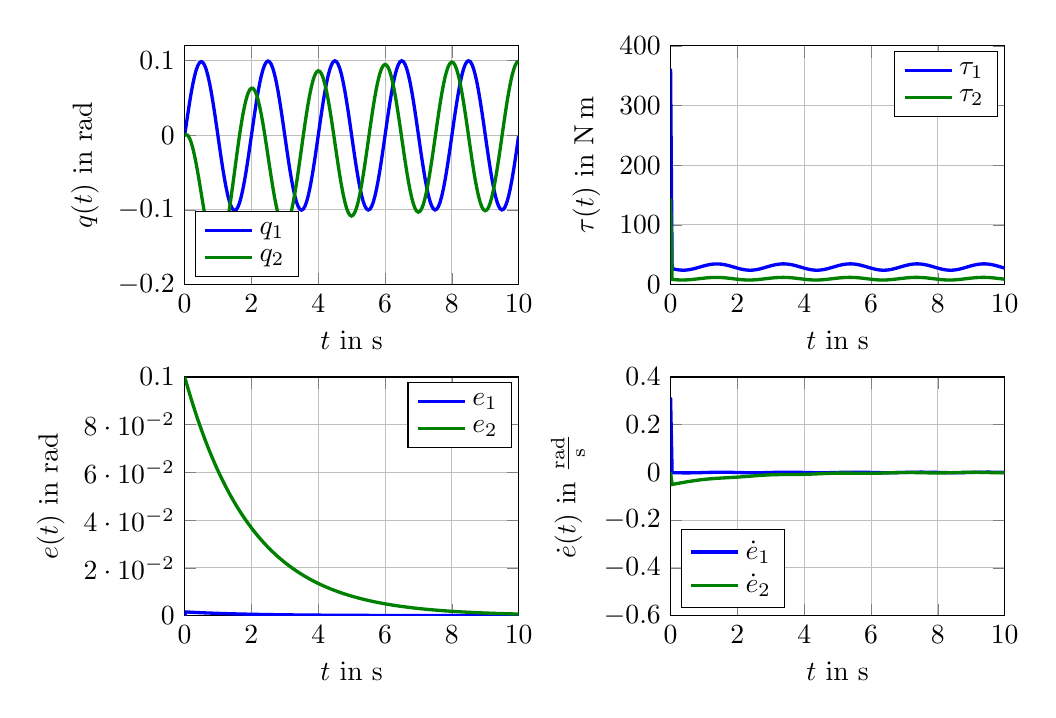
\begin{tikzpicture}

\begin{axis}[%
width=0.35\textwidth,
height=0.25\textwidth,
scale only axis,
xmin=0,
xmax=10,
xlabel={$t$ in $\mathrm{s}$},
xmajorgrids,
ymin=-0.2,
ymax=0.12,
ylabel={$q(t)$ in $\mathrm{rad}$},
ymajorgrids,
name=plot1,
legend style={at={(0.03,0.03)},anchor=south west,draw=black,fill=white,legend cell align=left}
]
\addplot [
color=blue,
solid,
line width=1.2pt
]
table[row sep=crcr]{
0 0\\
0.0464989243692912 0.0130139772805253\\
0.0964989243692912 0.0283496248424032\\
0.146498924369291 0.0429493759192578\\
0.196498924369291 0.056454528553765\\
0.246498924369291 0.0685334579064101\\
0.296498924369291 0.0788896348019371\\
0.346498924369291 0.0872689278165768\\
0.396498924369291 0.0934658613848978\\
0.446498924369292 0.0973286758243879\\
0.496498924369292 0.0987630646835022\\
0.546498924369292 0.0977344973875926\\
0.596498924369292 0.0942690699917881\\
0.646498924369292 0.0884528630927747\\
0.696498924369292 0.0804298227101259\\
0.746498924369292 0.0703982163172098\\
0.796498924369292 0.0586057512862456\\
0.846498924369292 0.0453434759478733\\
0.896498924369292 0.0309386134416665\\
0.946498924369292 0.0157465048122392\\
0.996498924369292 0.000141859738920696\\
1.04649892436929 -0.0154904696646734\\
1.09649892436928 -0.0307649648012516\\
1.14649892436928 -0.0453049329610427\\
1.19649892436927 -0.05875178237966\\
1.24649892436926 -0.0707738515996956\\
1.29649892436926 -0.0810745757276351\\
1.34649892436925 -0.0893997885055255\\
1.39649892436925 -0.095543980395945\\
1.44649892436924 -0.0993553585852432\\
1.49649892436924 -0.100739584310778\\
1.54649892436923 -0.0996620954865459\\
1.59649892436923 -0.0961489574362707\\
1.64649892436922 -0.0902862207858764\\
1.69649892436922 -0.0822178023259909\\
1.74649892436921 -0.0721419410244929\\
1.7964989243692 -0.0603063164536612\\
1.8464989243692 -0.0470019498322819\\
1.89649892436919 -0.0325560378591294\\
1.94649892436919 -0.0173238957924639\\
1.99649892436918 -0.00168020816350804\\
2.04649892436918 0.0139901974397796\\
2.09649892436917 0.0293018263387213\\
2.14649892436917 0.0438780091501417\\
2.19649892436916 0.0573601768588854\\
2.24649892436915 0.0694166901937013\\
2.29649892436915 0.0797510058980945\\
2.34649892436914 0.0881089788155862\\
2.39649892436914 0.0942851199879386\\
2.44649892436913 0.0981276566713229\\
2.49649892436913 0.0995422696761629\\
2.54649892436912 0.0984944160050627\\
2.59649892436912 0.095010179597883\\
2.64649892436911 0.0891756292359112\\
2.69649892436911 0.0811346994157687\\
2.7464989243691 0.0710856463730803\\
2.79649892436909 0.0592761665204714\\
2.84649892436909 0.0459972975002529\\
2.89649892436908 0.0315762520282196\\
2.94649892436908 0.0163683609832096\\
2.99649892436907 0.000748324130392767\\
3.04649892436907 -0.0148990160853857\\
3.09649892436906 -0.0301881504962893\\
3.14649892436906 -0.0447423955886106\\
3.19649892436905 -0.0582031685664112\\
3.24649892436904 -0.0702388167187504\\
3.29649892436904 -0.0805527836820939\\
3.34649892436903 -0.0888909115173405\\
3.39649892436903 -0.0950476988000171\\
3.44649892436902 -0.098871360628616\\
3.49649892436902 -0.100267565956801\\
3.54649892436901 -0.099201760223886\\
3.59649892436901 -0.09570001609265\\
3.646498924369 -0.0898483913464211\\
3.696498924369 -0.0817908097560754\\
3.74649892436899 -0.0717255170969697\\
3.79649892436898 -0.0599001995803665\\
3.84649892436898 -0.0466058848997118\\
3.89649892436897 -0.0321697760681832\\
3.94649892436897 -0.0169471945021545\\
3.99649892436896 -0.00131283073853994\\
4.04649892436898 0.0143484817776589\\
4.09649892436899 0.0296512426556911\\
4.14649892436901 0.0442187769416892\\
4.19649892436903 0.0576925101876878\\
4.24649892436904 0.0697407978240954\\
4.29649892436906 0.0800670914272175\\
4.34649892436908 0.088417240801271\\
4.39649892436909 0.0945857520734435\\
4.44649892436911 0.0984208477069742\\
4.49649892436913 0.099828203837986\\
4.54649892436914 0.0987732729104778\\
4.59649892436916 0.0952821344185367\\
4.64649892436918 0.0894408528077155\\
4.69649892436919 0.0813933583462165\\
4.74649892436921 0.0713379031459042\\
4.79649892436923 0.0595221795977127\\
4.84649892436924 0.0462372214218037\\
4.89649892436926 0.0318102375089016\\
4.94649892436928 0.0165965550074497\\
4.99649892436929 0.000970870044555252\\
5.04649892436931 -0.0146819784829521\\
5.09649892436933 -0.0299764848674334\\
5.14649892436934 -0.044535968969734\\
5.19649892436936 -0.0580018512849437\\
5.24649892436938 -0.0700424823116929\\
5.2964989243694 -0.080361308816577\\
5.34649892436941 -0.08870417591315\\
5.39649892436943 -0.0948655851540363\\
5.44649892436945 -0.0986937545411389\\
5.49649892436946 -0.100094355859669\\
5.54649892436948 -0.0990328373104035\\
5.5964989243695 -0.0955352742492346\\
5.64649892436951 -0.0896877270859451\\
5.69649892436953 -0.0816341221528582\\
5.74649892436955 -0.0715727077233779\\
5.79649892436956 -0.0597511724449843\\
5.84649892436958 -0.0464605463870412\\
5.8964989243696 -0.032028034879837\\
5.94649892436961 -0.0168089615995042\\
5.99649892436963 -0.00117801928678429\\
6.04649892436965 0.0144799564640424\\
6.09649892436966 0.0297794631661435\\
6.14649892436968 0.0443438238214517\\
6.1964989243697 0.0578144619883982\\
6.24649892436971 0.0698597311531327\\
6.29649892436973 0.0801830809958252\\
6.34649892436975 0.0885303594714891\\
6.39649892436976 0.0946960709038787\\
6.44649892436978 0.0985284359974374\\
6.4964989243698 0.099933129173025\\
6.54649892436981 0.0988756012018326\\
6.59649892436983 0.0953819299465433\\
6.64649892436985 0.0895381782616859\\
6.69649892436986 0.0814882748638181\\
6.74649892436988 0.0714304703515658\\
6.7964989243699 0.0596124556400783\\
6.84649892436991 0.0463252630102607\\
6.89649892436993 0.0318960999492041\\
6.94649892436995 0.0166802922364601\\
6.99649892436996 0.00105253466412617\\
7.04649892436998 -0.0146023351729347\\
7.09649892437 -0.0298988128368249\\
7.14649892437001 -0.0444602194267034\\
7.19649892437003 -0.057927976645324\\
7.24649892437005 -0.0699704361690896\\
7.29649892437006 -0.080291045913217\\
7.34649892437008 -0.0886356521114514\\
7.3964989243701 -0.094798757408883\\
7.44649892437011 -0.0986285808728398\\
7.49649892437013 -0.100030795327588\\
7.54649892437015 -0.0989708499872413\\
7.59649892437016 -0.0954748211959471\\
7.64649892437018 -0.089628770327283\\
7.6964989243702 -0.0815766246535116\\
7.74649892437021 -0.0715166333647115\\
7.79649892437023 -0.0596964860023487\\
7.84649892437025 -0.046407213507645\\
7.89649892437026 -0.0319760220611675\\
7.94649892437028 -0.0167582361682814\\
7.9964989243703 -0.00112854937843619\\
8.04649892437027 0.0145282019253962\\
8.09649892437024 0.0298265144872139\\
8.14649892437022 0.0443897105588181\\
8.19649892437019 0.0578592129670756\\
8.24649892437016 0.0699033744846791\\
8.29649892437013 0.0802256440960004\\
8.34649892437011 0.0885718690774766\\
8.39649892437008 0.0947365530910815\\
8.44649892437005 0.0985679161958578\\
8.49649892437002 0.0999716321832392\\
8.54649892437 0.0989131512105692\\
8.59649892436997 0.0954185505418774\\
8.64649892436994 0.0895738924478558\\
8.69649892436991 0.0815231050756763\\
8.74649892436988 0.0714644384686716\\
8.79649892436986 0.0596455830004422\\
8.84649892436983 0.0463575704237481\\
8.8964989243698 0.0319276077106077\\
8.94649892436977 0.0167110201382482\\
8.99649892436975 0.00108250200887634\\
9.04649892436972 -0.0145731095604106\\
9.09649892436969 -0.0298703105976552\\
9.14649892436966 -0.0444324226564239\\
9.19649892436964 -0.0579008678826308\\
9.24649892436961 -0.06994399838487\\
9.29649892436958 -0.0802652624998522\\
9.34649892436955 -0.0886105068723839\\
9.39649892436952 -0.0947742345484417\\
9.4464989243695 -0.0986046649863179\\
9.49649892436947 -0.100007471391565\\
9.54649892436944 -0.0989481033501468\\
9.59649892436941 -0.0954526375688556\\
9.64649892436939 -0.0896071357749384\\
9.69649892436936 -0.0815555255855731\\
9.74649892436933 -0.0714960565272165\\
9.7964989243693 -0.0596764184693867\\
9.84649892436927 -0.046387642673238\\
9.89649892436925 -0.0319569356313512\\
9.94649892436922 -0.0167396221533825\\
9.99649892436919 -0.00111039608554093\\
};
\addlegendentry{$q_1$};

\addplot [
color=green!50!black,
solid,
line width=1.2pt
]
table[row sep=crcr]{
0 0\\
0.0464989243692912 0.000992688555967006\\
0.0964989243692912 -7.82714990113225e-05\\
0.146498924369291 -0.00355925436415988\\
0.196498924369291 -0.00930487065837628\\
0.246498924369291 -0.0171154222827053\\
0.296498924369291 -0.0267418066481844\\
0.346498924369291 -0.0378916147409276\\
0.396498924369291 -0.0502362964168621\\
0.446498924369292 -0.0634192164720273\\
0.496498924369292 -0.0770644030999373\\
0.546498924369292 -0.0907857732991706\\
0.596498924369292 -0.104196608050764\\
0.646498924369292 -0.116919043935332\\
0.696498924369292 -0.128593347455515\\
0.746498924369292 -0.138886743680365\\
0.796498924369292 -0.147501581802801\\
0.846498924369292 -0.154182636529129\\
0.896498924369292 -0.15872336549875\\
0.946498924369292 -0.160970968638604\\
0.996498924369292 -0.160830124857669\\
1.04649892436929 -0.158265314055518\\
1.09649892436928 -0.153301667253595\\
1.14649892436928 -0.146024323900792\\
1.19649892436927 -0.136576312163564\\
1.24649892436926 -0.125155004380264\\
1.29649892436926 -0.112007234943896\\
1.34649892436925 -0.0974232008132994\\
1.39649892436925 -0.0817292948288478\\
1.44649892436924 -0.0652800482869807\\
1.49649892436924 -0.0484493811612132\\
1.54649892436923 -0.0316213754056314\\
1.59649892436923 -0.0151807985204853\\
1.64649892436922 0.000496389290830145\\
1.69649892436922 0.0150523106397828\\
1.74649892436921 0.028156000763053\\
1.7964989243692 0.0395115742170954\\
1.8464989243692 0.0488655273766224\\
1.89649892436919 0.0560129969358249\\
1.94649892436919 0.0608028203175606\\
1.99649892436918 0.0631412733964908\\
2.04649892436918 0.0629943935108143\\
2.09649892436917 0.0603888305718968\\
2.14649892436917 0.0554112053239728\\
2.19649892436916 0.0482059905647825\\
2.24649892436915 0.0389719675073904\\
2.29649892436915 0.0279573445479613\\
2.34649892436914 0.015453658640062\\
2.39649892436914 0.00178860945211603\\
2.44649892436913 -0.012681997237145\\
2.49649892436913 -0.0275829985170708\\
2.54649892436912 -0.0425291002608115\\
2.59649892436912 -0.0571343527982652\\
2.64649892436911 -0.0710216430164845\\
2.69649892436911 -0.0838319691534521\\
2.7464989243691 -0.0952332699021246\\
2.79649892436909 -0.10492859041617\\
2.84649892436909 -0.112663384136675\\
2.89649892436908 -0.118231770638222\\
2.94649892436908 -0.121481595399141\\
2.99649892436907 -0.122318166901532\\
3.04649892436907 -0.120706579035306\\
3.09649892436906 -0.116672561615156\\
3.14649892436906 -0.11030183806228\\
3.19649892436905 -0.101738006061338\\
3.24649892436904 -0.0911789933725442\\
3.29649892436904 -0.0788721760633222\\
3.34649892436903 -0.0651082793597579\\
3.39649892436903 -0.0502142112941443\\
3.44649892436902 -0.0345450056031453\\
3.49649892436902 -0.0184750722644267\\
3.54649892436901 -0.00238897110796137\\
3.59649892436901 0.0133280643181872\\
3.646498924369 0.0282996192981228\\
3.696498924369 0.04216737318061\\
3.74649892436899 0.0545999289109757\\
3.79649892436898 0.0653009794541156\\
3.84649892436898 0.0740166100281433\\
3.89649892436897 0.0805415563473314\\
3.94649892436897 0.0847242647794135\\
3.99649892436896 0.0864706298230688\\
4.04649892436898 0.0857463168800841\\
4.09649892436899 0.082577613131341\\
4.14649892436901 0.0770507855686591\\
4.19649892436903 0.0693099619932141\\
4.24649892436904 0.0595535871606364\\
4.29649892436906 0.0480295413374324\\
4.34649892436908 0.0350290414691626\\
4.39649892436909 0.0208794751368742\\
4.44649892436911 0.00593634375650618\\
4.49649892436913 -0.00942548659069348\\
4.54649892436914 -0.0248210112603492\\
4.59649892436916 -0.0398645628997513\\
4.64649892436918 -0.0541793037256082\\
4.69649892436919 -0.0674065004907778\\
4.74649892436921 -0.0792143537569863\\
4.79649892436923 -0.0893061640650656\\
4.84649892436924 -0.097427633922091\\
4.89649892436926 -0.103373125803912\\
4.94649892436928 -0.106990722077992\\
4.99649892436929 -0.108185962252241\\
5.04649892436931 -0.106924165524176\\
5.09649892436933 -0.103231281439432\\
5.14649892436934 -0.0971932477115097\\
5.19649892436936 -0.0889538710133486\\
5.24649892436938 -0.0787112829207004\\
5.2964989243694 -0.0667130582718171\\
5.34649892436941 -0.0532501161437665\\
5.39649892436943 -0.0386495536217501\\
5.44649892436945 -0.0232665888160257\\
5.49649892436946 -0.00747581151435744\\
5.54649892436948 0.00833804309372586\\
5.5964989243695 0.0237895704409906\\
5.64649892436951 0.0385021890253259\\
5.69649892436953 0.0521174155374654\\
5.74649892436955 0.0643036942907113\\
5.79649892436956 0.0747645635442913\\
5.84649892436958 0.0832459576398251\\
5.8964989243696 0.0895424651494885\\
5.94649892436961 0.0935023889408841\\
5.99649892436963 0.0950314835643818\\
6.04649892436965 0.0940952779373694\\
6.09649892436966 0.0907199261345026\\
6.14649892436968 0.0849915653359337\\
6.1964989243697 0.0770541967441847\\
6.24649892436971 0.0671061416497198\\
6.29649892436973 0.0553951599098089\\
6.34649892436975 0.0422123510410666\\
6.39649892436976 0.0278849881021194\\
6.44649892436978 0.0127684608210698\\
6.4964989243698 -0.00276247364424618\\
6.54649892436981 -0.0183229168768634\\
6.59649892436983 -0.0335273051222113\\
6.64649892436985 -0.0479989016309434\\
6.69649892436986 -0.0613790716891366\\
6.74649892436988 -0.0733361119529059\\
6.7964989243699 -0.0835734166790065\\
6.84649892436991 -0.0918367797708414\\
6.89649892436993 -0.0979206528384049\\
6.94649892436995 -0.101673205177117\\
6.99649892436996 -0.103000061071257\\
7.04649892436998 -0.101866622396383\\
7.09649892437 -0.098298919329779\\
7.14649892437001 -0.0923829682208519\\
7.19649892437003 -0.0842626524321023\\
7.24649892437005 -0.074136178330673\\
7.29649892437006 -0.0622511936950193\\
7.34649892437008 -0.0488986887370434\\
7.3964989243701 -0.0344058299160984\\
7.44649892437011 -0.0191279029994893\\
7.49649892437013 -0.00343956375742449\\
7.54649892437015 0.0122743882712779\\
7.59649892437016 0.0276284857628268\\
7.64649892437018 0.0422460860118632\\
7.6964989243702 0.0557686460207363\\
7.74649892437021 0.0678645518917315\\
7.79649892437023 0.0782372851138612\\
7.84649892437025 0.0866327246636697\\
7.89649892437026 0.0928454051186174\\
7.94649892437028 0.0967235766880337\\
7.9964989243703 0.098172942567379\\
8.04649892437027 0.0971589815902351\\
8.09649892437024 0.0937077989870949\\
8.14649892437022 0.087905484302905\\
8.19649892437019 0.0798959922840169\\
8.24649892437016 0.0698775989145777\\
8.29649892437013 0.0580980198669316\\
8.34649892437011 0.0448483115664047\\
8.39649892437008 0.0304557050469019\\
8.44649892437005 0.0152755490519727\\
8.49649892437002 -0.000317439230677095\\
8.54649892437 -0.0159384003648979\\
8.59649892436997 -0.0312018086121071\\
8.64649892436994 -0.0457309642979991\\
8.69649892436991 -0.0591672688660344\\
8.74649892436988 -0.0711790542347675\\
8.79649892436986 -0.0814697490506002\\
8.84649892436983 -0.0897851807553917\\
8.8964989243698 -0.0959198336674704\\
8.94649892436977 -0.0997219089810148\\
8.99649892436975 -0.101097062089525\\
9.04649892436972 -0.100010725207786\\
9.09649892436969 -0.096488958101369\\
9.14649892436966 -0.0906178059756201\\
9.19649892436964 -0.0825411803347547\\
9.24649892436961 -0.072457314991085\\
9.29649892436958 -0.0606138844889305\\
9.34649892436955 -0.0473019051435665\\
9.39649892436952 -0.0328485688716251\\
9.4464989243695 -0.0176091862675884\\
9.49649892436947 -0.00195843731433589\\
9.54649892436944 0.0137188548359395\\
9.59649892436941 0.0290371998305348\\
9.64649892436939 0.0436199325051755\\
9.69649892436936 0.0571084879591836\\
9.74649892436933 0.0691712309339467\\
9.7964989243693 0.0795116220862903\\
9.84649892436927 0.087875520076196\\
9.89649892436925 0.0940574396674237\\
9.94649892436922 0.0979056117460181\\
9.99649892436919 0.0993257206624319\\
};
\addlegendentry{$q_2$};

\end{axis}

\begin{axis}[%
width=0.35\textwidth,
height=0.25\textwidth,
scale only axis,
xmin=0,
xmax=10,
xlabel={$t$ in $\mathrm{s}$},
xmajorgrids,
ymin=0,
ymax=0.1,
ylabel={$e(t)$ in $\mathrm{rad}$},
ymajorgrids,
name=plot3,
at=(plot1.below south west),
anchor=above north west,
legend style={draw=black,fill=white,legend cell align=left}
]
\addplot [
color=blue,
solid,
line width=1.2pt
]
table[row sep=crcr]{
0 0\\
0.0464989243692912 0.00154219107722954\\
0.0964989243692912 0.00150416387022681\\
0.146498924369291 0.00146693379109807\\
0.196498924369291 0.0014306251999672\\
0.246498924369291 0.00139521529547039\\
0.296498924369291 0.00136068183390074\\
0.346498924369291 0.00132700312211283\\
0.396498924369291 0.00129415800389589\\
0.446498924369292 0.00126212584668386\\
0.496498924369292 0.00123088652859459\\
0.546498924369292 0.00120042042578958\\
0.596498924369292 0.00117070840014682\\
0.646498924369292 0.00114173178723881\\
0.696498924369292 0.00111347238460743\\
0.746498924369292 0.00108591244033038\\
0.796498924369292 0.00105903464186916\\
0.846498924369292 0.00103282210519401\\
0.896498924369292 0.00100725836417785\\
0.946498924369292 0.00098232736025235\\
0.996498924369292 0.000958013432320401\\
1.04649892436929 0.00093430130691999\\
1.09649892436928 0.000911176088624607\\
1.14649892436928 0.000888623250691147\\
1.19649892436927 0.000866628625933112\\
1.24649892436926 0.000845178397821028\\
1.29649892436926 0.000824259091803212\\
1.34649892436925 0.00080385756684144\\
1.39649892436925 0.000783961007155637\\
1.44649892436924 0.000764556914174055\\
1.49649892436924 0.000745633098681073\\
1.54649892436923 0.000727177673160898\\
1.59649892436923 0.000709179044329669\\
1.64649892436922 0.000691625905853047\\
1.69649892436922 0.000674507231243682\\
1.74649892436921 0.000657812266934663\\
1.7964989243692 0.000641530525524445\\
1.8464989243692 0.00062565177918867\\
1.89649892436919 0.000610166053255666\\
1.94649892436919 0.000595063619940005\\
1.99649892436918 0.000580334992232428\\
2.04649892436918 0.000565970917939661\\
2.09649892436917 0.000551962373872759\\
2.14649892436917 0.000538300560178805\\
2.19649892436916 0.000524976894813296\\
2.24649892436915 0.000511983008148503\\
2.29649892436915 0.000499310737716696\\
2.34649892436914 0.000486952123081877\\
2.39649892436914 0.000474899400839737\\
2.44649892436913 0.000463144999740553\\
2.49649892436913 0.000451681535933293\\
2.54649892436912 0.000440501808327276\\
2.59649892436912 0.000429598794068356\\
2.64649892436911 0.000418965644127509\\
2.69649892436911 0.000408595678998563\\
2.7464989243691 0.000398482384502075\\
2.79649892436909 0.00038861940769308\\
2.84649892436909 0.000379000552870934\\
2.89649892436908 0.000369619777686819\\
2.94649892436908 0.000360471189348392\\
2.99649892436907 0.000351549040917407\\
3.04649892436907 0.0003428477277006\\
3.09649892436906 0.000334361783728296\\
3.14649892436906 0.000326085878321114\\
3.19649892436905 0.000318014812740762\\
3.24649892436904 0.000310143516925293\\
3.29649892436904 0.000302467046303337\\
3.34649892436903 0.000294980578688486\\
3.39649892436903 0.00028767941124988\\
3.44649892436902 0.000280558957558394\\
3.49649892436902 0.0002736147447049\\
3.54649892436901 0.000266842410490936\\
3.59649892436901 0.000260237700688365\\
3.646498924369 0.000253796466366973\\
3.696498924369 0.000247514661288153\\
3.74649892436899 0.000241388339363185\\
3.79649892436898 0.000235413652174214\\
3.84649892436898 0.000229586846557286\\
3.89649892436897 0.00022390426224398\\
3.94649892436897 0.000218362329562516\\
3.99649892436896 0.000212957567195114\\
4.04649892436898 0.000207686579998336\\
4.09649892436899 0.00020254605684978\\
4.14649892436901 0.000197532768587701\\
4.19649892436903 0.000192643565976806\\
4.24649892436904 0.000187875377729588\\
4.29649892436906 0.000183225208577151\\
4.34649892436908 0.000178690137387416\\
4.39649892436909 0.000174267315330309\\
4.44649892436911 0.000169953964088074\\
4.49649892436913 0.000165747374110209\\
4.54649892436914 0.000161644902911123\\
4.59649892436916 0.000157643973410462\\
4.64649892436918 0.000153742072313903\\
4.69649892436919 0.00014993674853464\\
4.74649892436921 0.000146225611653755\\
4.79649892436923 0.000142606330418196\\
4.84649892436924 0.000139076631276866\\
4.89649892436926 0.000135634296951778\\
4.94649892436928 0.00013227716504614\\
4.99649892436929 0.000129003126684962\\
5.04649892436931 0.000125810125190943\\
5.09649892436933 0.000122696154792344\\
5.14649892436934 0.00011965925936315\\
5.19649892436936 0.000116697531193477\\
5.24649892436938 0.000113809109792973\\
5.2964989243694 0.000110992180719791\\
5.34649892436941 0.000108244974442936\\
5.39649892436943 0.000105565765228924\\
5.44649892436945 0.000102952870059111\\
5.49649892436946 0.000100404647571328\\
5.54649892436948 9.79194970297803e-05\\
5.5964989243695 9.54958573187448e-05\\
5.64649892436951 9.31322059622569e-05\\
5.69649892436953 9.08270581678333e-05\\
5.74649892436955 8.85789658934266e-05\\
5.79649892436956 8.63865169376254e-05\\
5.84649892436958 8.42483340538075e-05\\
5.8964989243696 8.21630740828472e-05\\
5.94649892436961 8.01294271119135e-05\\
5.99649892436963 7.81461156488653e-05\\
6.04649892436965 7.62118938225868e-05\\
6.09649892436966 7.43255465975382e-05\\
6.14649892436968 7.24858890132976e-05\\
6.1964989243697 7.06917654374611e-05\\
6.24649892436971 6.89420488423353e-05\\
6.29649892436973 6.72356400945595e-05\\
6.34649892436975 6.55714672666563e-05\\
6.39649892436976 6.39484849621341e-05\\
6.44649892436978 6.23656736600114e-05\\
6.4964989243698 6.08220390734687e-05\\
6.54649892436981 5.93166115258198e-05\\
6.59649892436983 5.78484453412215e-05\\
6.64649892436985 5.64166182502879e-05\\
6.69649892436986 5.5020230811581e-05\\
6.74649892436988 5.36584058453832e-05\\
6.7964989243699 5.2330287884296e-05\\
6.84649892436991 5.10350426338596e-05\\
6.89649892436993 4.97718564506783e-05\\
6.94649892436995 4.85399358289215e-05\\
6.99649892436996 4.73385069044677e-05\\
7.04649892436998 4.6166814966029e-05\\
7.09649892437 4.50241239838382e-05\\
7.14649892437001 4.39097161445273e-05\\
7.19649892437003 4.2822891402873e-05\\
7.24649892437005 4.17629670396019e-05\\
7.29649892437006 4.07292772346829e-05\\
7.34649892437008 3.97211726470281e-05\\
7.3964989243701 3.8738020008533e-05\\
7.44649892437011 3.77792017249162e-05\\
7.49649892437013 3.6844115488141e-05\\
7.54649892437015 3.5932173898176e-05\\
7.59649892437016 3.50428040939849e-05\\
7.64649892437018 3.41754473933836e-05\\
7.6964989243702 3.33295589427518e-05\\
7.74649892437021 3.25046073736679e-05\\
7.79649892437023 3.17000744705226e-05\\
7.84649892437025 3.0915454843343e-05\\
7.89649892437026 3.01502556122879e-05\\
7.94649892437028 2.94039960956893e-05\\
7.9964989243703 2.86762075106877e-05\\
8.04649892437027 2.79664326634302e-05\\
8.09649892437024 2.72742257017705e-05\\
8.14649892437022 2.65991517984232e-05\\
8.19649892437019 2.59407868866413e-05\\
8.24649892437016 2.52987173967878e-05\\
8.29649892437013 2.46725399952602e-05\\
8.34649892437011 2.40618613316923e-05\\
8.39649892437008 2.34662977910971e-05\\
8.44649892437005 2.28854752538504e-05\\
8.49649892437002 2.23190288601016e-05\\
8.54649892437 2.17666027808455e-05\\
8.59649892436997 2.12278499941015e-05\\
8.64649892436994 2.07024320672544e-05\\
8.69649892436991 2.01900189442938e-05\\
8.74649892436988 1.96902887382722e-05\\
8.79649892436986 1.92029275300834e-05\\
8.84649892436983 1.87276291697402e-05\\
8.8964989243698 1.82640950851798e-05\\
8.94649892436977 1.7812034094046e-05\\
8.99649892436975 1.73711622221805e-05\\
9.04649892436972 1.69412025231575e-05\\
9.09649892436969 1.65218849056993e-05\\
9.14649892436966 1.61129459634035e-05\\
9.19649892436964 1.57141288105178e-05\\
9.24649892436961 1.53251829185797e-05\\
9.29649892436958 1.4945863960461e-05\\
9.34649892436955 1.45759336564882e-05\\
9.39649892436952 1.42151596247003e-05\\
9.4464989243695 1.38633152353268e-05\\
9.49649892436947 1.3520179467541e-05\\
9.54649892436944 1.31855367713901e-05\\
9.59649892436941 1.28591769321534e-05\\
9.64649892436939 1.25408949379624e-05\\
9.69649892436936 1.2230490851653e-05\\
9.74649892436933 1.1927769684561e-05\\
9.7964989243693 1.16325412746962e-05\\
9.84649892436927 1.13446201659637e-05\\
9.89649892436925 1.10638254933598e-05\\
9.94649892436922 1.07899808682761e-05\\
9.99649892436919 1.05229142683232e-05\\
};
\addlegendentry{$e_1$};

\addplot [
color=green!50!black,
solid,
line width=1.2pt
]
table[row sep=crcr]{
0 0.1\\
0.0464989243692912 0.0979422292574152\\
0.0964989243692912 0.0955180498909462\\
0.146498924369291 0.0931538492441734\\
0.196498924369291 0.0908481657531097\\
0.246498924369291 0.0885995510402455\\
0.296498924369291 0.0864065925762992\\
0.346498924369291 0.084267912793995\\
0.396498924369291 0.0821821682227066\\
0.446498924369292 0.080148048644519\\
0.496498924369292 0.0781642762711785\\
0.546498924369292 0.0762296049414156\\
0.596498924369292 0.0743428193381341\\
0.646498924369292 0.0725027342249759\\
0.696498924369292 0.0707081937017825\\
0.746498924369292 0.0689580704784845\\
0.796498924369292 0.0672512651669631\\
0.846498924369292 0.065586705590439\\
0.896498924369292 0.0639633461099558\\
0.946498924369292 0.062380166967532\\
0.996498924369292 0.0608361736455727\\
1.04649892436929 0.0593303962421352\\
1.09649892436928 0.0578618888616592\\
1.14649892436928 0.0564297290207764\\
1.19649892436927 0.0550330170688264\\
1.24649892436926 0.0536708756227174\\
1.29649892436926 0.0523424490157729\\
1.34649892436925 0.0510469027602215\\
1.39649892436925 0.0497834230229905\\
1.44649892436924 0.0485512161144739\\
1.49649892436924 0.0473495079899549\\
1.54649892436923 0.0461775437633677\\
1.59649892436923 0.0450345872330957\\
1.64649892436922 0.0439199204195058\\
1.69649892436922 0.0428328431139299\\
1.74649892436921 0.0417726724388092\\
1.7964989243692 0.0407387424187261\\
1.8464989243692 0.0397304035620536\\
1.89649892436919 0.0387470224529588\\
1.94649892436919 0.0377879813535056\\
1.99649892436918 0.0368526778156055\\
2.04649892436918 0.0359405243025732\\
2.09649892436917 0.0350509478200493\\
2.14649892436917 0.0341833895560583\\
2.19649892436916 0.0333373045299748\\
2.24649892436915 0.0325121612501799\\
2.29649892436915 0.0317074413801893\\
2.34649892436914 0.0309226394130465\\
2.39649892436914 0.0301572623537741\\
2.44649892436913 0.0294108294096859\\
2.49649892436913 0.0286828716883637\\
2.54649892436912 0.0279729319031094\\
2.59649892436912 0.0272805640856877\\
2.64649892436911 0.0266053333061794\\
2.69649892436911 0.0259468153997675\\
2.7464989243691 0.0253045967002871\\
2.79649892436909 0.0246782737803686\\
2.84649892436909 0.0240674531980148\\
2.89649892436908 0.0234717512494488\\
2.94649892436908 0.0228907937280802\\
2.99649892436907 0.0223242156894363\\
3.04649892436907 0.0217716612219131\\
3.09649892436906 0.0212327832231992\\
3.14649892436906 0.0207072431822334\\
3.19649892436905 0.0201947109665608\\
3.24649892436904 0.0196948646149497\\
3.29649892436904 0.0192073901351438\\
3.34649892436903 0.0187319813066187\\
3.39649892436903 0.0182683394882214\\
3.44649892436902 0.0178161734305703\\
3.49649892436902 0.0173751990930993\\
3.54649892436901 0.0169451394656292\\
3.59649892436901 0.0165257243943572\\
3.646498924369 0.0161166904121512\\
3.696498924369 0.0157177805730463\\
3.74649892436899 0.0153287442908371\\
3.79649892436898 0.0149493371816646\\
3.84649892436898 0.0145793209105007\\
3.89649892436897 0.0142184630414303\\
3.94649892436897 0.0138665368916413\\
3.99649892436896 0.0135233213890268\\
4.04649892436898 0.0131886009333125\\
4.09649892436899 0.0128621652606218\\
4.14649892436901 0.0125438093113936\\
4.19649892436903 0.0122333331015674\\
4.24649892436904 0.0119305415969582\\
4.29649892436906 0.0116352445907405\\
4.34649892436908 0.0113472565839643\\
4.39649892436909 0.0110663966690291\\
4.44649892436911 0.0107924884160415\\
4.49649892436913 0.0105253597619863\\
4.54649892436914 0.01026484290264\\
4.59649892436916 0.0100107741871604\\
4.64649892436918 0.00976299401528432\\
4.69649892436919 0.00952134673707045\\
4.74649892436921 0.00928568055512381\\
4.79649892436923 0.00905584742923968\\
4.84649892436924 0.00883170298340832\\
4.89649892436926 0.00861310641512091\\
4.94649892436928 0.00839992040692113\\
4.99649892436929 0.00819201104014461\\
5.04649892436931 0.00798924771079493\\
5.09649892436933 0.00779150304750059\\
5.14649892436934 0.00759865283150354\\
5.19649892436936 0.00741057591862793\\
5.24649892436938 0.00722715416317905\\
5.2964989243694 0.0070482723437284\\
5.34649892436941 0.0068738180907324\\
5.39649892436943 0.00670368181594636\\
5.44649892436945 0.00653775664358133\\
5.49649892436946 0.00637593834316962\\
5.54649892436948 0.00621812526408693\\
5.5964989243695 0.00606421827170042\\
5.64649892436951 0.00591412068509188\\
5.69649892436953 0.00576773821632758\\
5.74649892436955 0.00562497891122633\\
5.79649892436956 0.00548575309159727\\
5.84649892436958 0.00534997329890639\\
5.8964989243696 0.00521755423933562\\
5.94649892436961 0.00508841273020452\\
5.99649892436963 0.00496246764771606\\
6.04649892436965 0.00483963987599666\\
6.09649892436966 0.00471985225739756\\
6.14649892436968 0.00460302954402568\\
6.1964989243697 0.00448909835047527\\
6.24649892436971 0.00437798710772794\\
6.29649892436973 0.00426962601819571\\
6.34649892436975 0.00416394701187432\\
6.39649892436976 0.00406088370358509\\
6.44649892436978 0.00396037135127089\\
6.4964989243698 0.00386234681532921\\
6.54649892436981 0.0037667485189466\\
6.59649892436983 0.00367351640942026\\
6.64649892436985 0.00358259192043146\\
6.69649892436986 0.00349391793525824\\
6.74649892436988 0.00340743875089339\\
6.7964989243699 0.00332310004305551\\
6.84649892436991 0.00324084883206135\\
6.89649892436993 0.00316063344954726\\
6.94649892436995 0.00308240350601068\\
6.99649892436996 0.00300610985915764\\
7.04649892436998 0.00293170458303212\\
7.09649892437 0.00285914093791009\\
7.14649892437001 0.002788373340939\\
7.19649892437003 0.00271935733750299\\
7.24649892437005 0.00265204957329852\\
7.29649892437006 0.00258640776709877\\
7.34649892437008 0.00252239068419532\\
7.3964989243701 0.00245995811049358\\
7.44649892437011 0.00239907082725193\\
7.49649892437013 0.0023396905864466\\
7.54649892437015 0.00228178008674259\\
7.59649892437016 0.00222530295006465\\
7.64649892437018 0.00217022369874265\\
7.6964989243702 0.00211650773322788\\
7.74649892437021 0.00206412131035597\\
7.79649892437023 0.00201303152215254\\
7.84649892437025 0.00196320627515896\\
7.89649892437026 0.00191461427027377\\
7.94649892437028 0.00186722498308999\\
7.9964989243703 0.00182100864472123\\
8.04649892437027 0.00177593622310229\\
8.09649892437024 0.00173197940475066\\
8.14649892437022 0.00168911057697936\\
8.19649892437019 0.00164730281055321\\
8.24649892437016 0.00160652984277151\\
8.29649892437013 0.00156676606097097\\
8.34649892437011 0.00152798648643587\\
8.39649892437008 0.00149016675870837\\
8.44649892437005 0.00145328312028397\\
8.49649892437002 0.00141731240168875\\
8.54649892437 0.0013822320069242\\
8.59649892436997 0.00134801989927436\\
8.64649892436994 0.00131465458746072\\
8.69649892436991 0.00128211511214327\\
8.74649892436988 0.00125038103275371\\
8.79649892436986 0.00121943241465636\\
8.84649892436983 0.00118924981662386\\
8.8964989243698 0.00115981427862559\\
8.94649892436977 0.00113110730991767\\
8.99649892436975 0.0011031108774269\\
9.04649892436972 0.00107580739442313\\
9.09649892436969 0.00104917970947145\\
9.14649892436966 0.00102321109565842\\
9.19649892436964 0.00099788524008379\\
9.24649892436961 0.000973186233614101\\
9.29649892436958 0.000949098560888255\\
9.34649892436955 0.000925607090571372\\
9.39649892436952 0.000902697065849854\\
9.4464989243695 0.000880354095160102\\
9.49649892436947 0.00085856414315015\\
9.54649892436944 0.000837313521861598\\
9.59649892436941 0.000816588882131798\\
9.64649892436939 0.000796377205206845\\
9.69649892436936 0.000776665794565555\\
9.74649892436933 0.000757442267942332\\
9.7964989243693 0.00073869454954964\\
9.84649892436927 0.00072041086249118\\
9.89649892436925 0.000702579721365476\\
9.94649892436922 0.000685189925049789\\
9.99649892436919 0.000668230549664445\\
};
\addlegendentry{$e_2$};

\end{axis}

\begin{axis}[%
width=0.35\textwidth,
height=0.25\textwidth,
scale only axis,
xmin=0,
xmax=10,
xlabel={$t$ in $\mathrm{s}$},
xmajorgrids,
ymin=-0.6,
ymax=0.4,
ylabel={$\dot{e}(t)$ in $\mathrm{\frac{rad}{s}}$},
ymajorgrids,
name=plot2,
at=(plot3.right of south east),
anchor=left of south west,
legend style={at={(0.03,0.03)},anchor=south west,draw=black,fill=white,legend cell align=left}
]
\addplot [
color=blue,
solid,
line width=1.2pt
]
table[row sep=crcr]{
0 0.314159265358979\\
0.0464989243692912 -0.000917088631238849\\
0.0964989243692912 -0.00110735978930432\\
0.146498924369291 -0.00125992619303666\\
0.196498924369291 -0.00140003533268779\\
0.246498924369291 -0.00152377905343723\\
0.296498924369291 -0.00162766217441004\\
0.346498924369291 -0.0017086896420985\\
0.396498924369291 -0.00176444000400315\\
0.446498924369292 -0.00179312476504583\\
0.496498924369292 -0.00179363216509752\\
0.546498924369292 -0.00176555429951067\\
0.596498924369292 -0.00170919691469729\\
0.646498924369292 -0.00162557163739688\\
0.696498924369292 -0.0015163708288248\\
0.746498924369292 -0.00138392568272516\\
0.796498924369292 -0.00123114859894957\\
0.846498924369292 -0.00106146125137402\\
0.896498924369292 -0.000878710121223647\\
0.946498924369292 -0.000687071575518838\\
0.996498924369292 -0.000490948827798487\\
1.04649892436929 -0.000294863318159699\\
1.09649892436928 -0.000103343187071336\\
1.14649892436928 7.91884110089014e-05\\
1.19649892436927 0.000248522404249052\\
1.24649892436926 0.000400767624081227\\
1.29649892436926 0.000532446793568481\\
1.34649892436925 0.000640582320056482\\
1.39649892436925 0.000722769779720259\\
1.44649892436924 0.000777237284672244\\
1.49649892436924 0.000802889270925047\\
1.54649892436923 0.000799333629095116\\
1.59649892436923 0.00076689150990536\\
1.64649892436922 0.000706589563127802\\
1.69649892436922 0.000620134801170985\\
1.74649892436921 0.000509872706334125\\
1.7964989243692 0.000378729613364215\\
1.8464989243692 0.000230140786124267\\
1.89649892436919 6.79659594563509e-05\\
1.94649892436919 -0.000103605574047427\\
1.99649892436918 -0.000280157995201535\\
2.04649892436918 -0.000457157570269984\\
2.09649892436917 -0.000630064169427347\\
2.14649892436917 -0.00079444294561315\\
2.19649892436916 -0.000946073423800375\\
2.24649892436915 -0.00108105331446989\\
2.29649892436915 -0.00119589449499305\\
2.34649892436914 -0.00128760879546866\\
2.39649892436914 -0.00135378147662629\\
2.44649892436913 -0.001392630590454\\
2.49649892436913 -0.00140305076184179\\
2.54649892436912 -0.00138464031312217\\
2.59649892436912 -0.0013377110635607\\
2.64649892436911 -0.00126328056244124\\
2.69649892436911 -0.0011630469469304\\
2.7464989243691 -0.00103934704376132\\
2.79649892436909 -0.000895098746350964\\
2.84649892436909 -0.000733729086167478\\
2.89649892436908 -0.000559089769420873\\
2.94649892436908 -0.000375362258790202\\
2.99649892436907 -0.000186954737348921\\
3.04649892436907 1.60650827468745e-06\\
3.09649892436906 0.000185788611037241\\
3.14649892436906 0.000361163806896381\\
3.19649892436905 0.000523518528528832\\
3.24649892436904 0.000668957223144612\\
3.29649892436904 0.000793998338101176\\
3.34649892436903 0.000895660110867197\\
3.39649892436903 0.000971534050950462\\
3.44649892436902 0.00101984430445209\\
3.49649892436902 0.0010394914395383\\
3.54649892436901 0.00103007957471267\\
3.59649892436901 0.000991926181949654\\
3.646498924369 0.000926054323327569\\
3.696498924369 0.000834167512362011\\
3.74649892436899 0.000718607819060774\\
3.79649892436898 0.000582298250337954\\
3.84649892436898 0.000428670824592803\\
3.89649892436897 0.000261582111532543\\
3.94649892436897 8.52183169568477e-05\\
3.99649892436896 -9.60077503400214e-05\\
4.04649892436898 -0.000277565292504778\\
4.09649892436899 -0.000454917042921998\\
4.14649892436901 -0.000623630946874676\\
4.19649892436903 -0.000779489252565047\\
4.24649892436904 -0.000918592326301176\\
4.29649892436906 -0.00103745463554455\\
4.34649892436908 -0.00113309053637742\\
4.39649892436909 -0.00120308775298991\\
4.44649892436911 -0.00124566673985864\\
4.49649892436913 -0.00125972446489427\\
4.54649892436914 -0.00124486153545977\\
4.59649892436916 -0.00120139199929335\\
4.64649892436918 -0.00113033557899175\\
4.69649892436919 -0.00103339253124413\\
4.74649892436921 -0.000912901749844791\\
4.79649892436923 -0.000771783144108917\\
4.84649892436924 -0.000613465711507\\
4.89649892436926 -0.00044180307558922\\
4.94649892436928 -0.000260978568919434\\
4.99649892436929 -7.54021981730912e-05\\
5.04649892436931 0.000110397971556375\\
5.09649892436933 0.000291887338779218\\
5.14649892436934 0.000464636447937594\\
5.19649892436936 0.00062443008205848\\
5.24649892436938 0.000767371079535839\\
5.2964989243694 0.000889976318728197\\
5.34649892436941 0.000989262506941313\\
5.39649892436943 0.00106281966139596\\
5.44649892436945 0.0011088704728389\\
5.49649892436946 0.00112631409010662\\
5.54649892436948 0.00111475324750054\\
5.5964989243695 0.0010745040670582\\
5.64649892436951 0.00100658829432909\\
5.69649892436953 0.000912708158889025\\
5.74649892436955 0.000795204478582917\\
5.79649892436956 0.000656999039157613\\
5.84649892436958 0.000501522668067633\\
5.8964989243696 0.00033263077355572\\
5.94649892436961 0.000154508428702127\\
5.99649892436963 -2.84326623796738e-05\\
6.04649892436965 -0.000211662779172783\\
6.09649892436966 -0.000390645705738435\\
6.14649892436968 -0.000560950412027972\\
6.1964989243697 -0.000718360145550878\\
6.24649892436971 -0.000858976247186144\\
6.29649892436973 -0.00097931413484692\\
6.34649892436975 -0.00107638909153882\\
6.39649892436976 -0.00114778974543667\\
6.44649892436978 -0.00119173743262214\\
6.4964989243698 -0.00120712998079606\\
6.54649892436981 -0.00119356883582464\\
6.59649892436983 -0.00115136886319994\\
6.64649892436985 -0.001081550583028\\
6.69649892436986 -0.000985815029771797\\
6.74649892436988 -0.000866501855744745\\
6.7964989243699 -0.000726531710010192\\
6.84649892436991 -0.000569334311474434\\
6.89649892436993 -0.000398763987267681\\
6.94649892436995 -0.000219004756120245\\
6.99649892436996 -3.44672938890622e-05\\
7.04649892436998 0.000150319681712807\\
7.09649892437 0.000330820932730291\\
7.14649892437001 0.000502606382892734\\
7.19649892437003 0.000661460209878451\\
7.24649892437005 0.000803484661715509\\
7.29649892437006 0.000925196041008214\\
7.34649892437008 0.00102361049356237\\
7.3964989243701 0.00109631748899\\
7.44649892437011 0.00114153918399148\\
7.49649892437013 0.00115817420656627\\
7.54649892437015 0.00114582478307967\\
7.59649892437016 0.00110480654019526\\
7.64649892437018 0.0010361407403601\\
7.6964989243702 0.000941529141994774\\
7.74649892437021 0.000823312103460011\\
7.79649892437023 0.000684410962383419\\
7.84649892437025 0.000528256109198377\\
7.89649892437026 0.000358702525937726\\
7.94649892437028 0.000179934870025877\\
7.9964989243703 -3.63555979487895e-06\\
8.04649892437027 -0.00018747943833719\\
8.09649892437024 -0.000367060935218988\\
8.14649892437022 -0.000537949396401838\\
8.19649892437019 -0.000695928436097504\\
8.24649892437016 -0.000837099752809961\\
8.29649892437013 -0.000957979113225427\\
8.34649892437011 -0.00105558214049251\\
8.39649892437008 -0.00112749779450717\\
8.44649892437005 -0.00117194773486259\\
8.49649892437002 -0.00118783010476297\\
8.54649892437 -0.00117474665777152\\
8.59649892436997 -0.00113301255945814\\
8.64649892436994 -0.00106364862258074\\
8.69649892436991 -0.000968356167009632\\
8.74649892436988 -0.00084947512340397\\
8.79649892436986 -0.000709926412280515\\
8.84649892436983 -0.000553140017280462\\
8.8964989243698 -0.000382970523718384\\
8.94649892436977 -0.00020360220211646\\
8.99649892436975 -1.94459738924735e-05\\
9.04649892436972 0.000164969203758525\\
9.09649892436969 0.000345107859326454\\
9.14649892436966 0.000516539688766193\\
9.19649892436964 0.000675048647620913\\
9.24649892436961 0.000816736767278003\\
9.29649892436958 0.000938120139067994\\
9.34649892436955 0.00103621470274773\\
9.39649892436952 0.00110860972698559\\
9.4464989243695 0.00115352717250412\\
9.49649892436947 0.00116986547618387\\
9.54649892436944 0.00115722667799546\\
9.59649892436941 0.00111592622282733\\
9.64649892436939 0.00104698519584182\\
9.69649892436936 0.000952105182572077\\
9.74649892436933 0.000833626372764268\\
9.7964989243693 0.000694469939609088\\
9.84649892436927 0.000538066113168201\\
9.89649892436925 0.000368269719077163\\
9.94649892436922 0.000189265262230731\\
9.99649892436919 5.46389261840696e-06\\
};
\addlegendentry{$\dot{e}_1$};

\addplot [
color=green!50!black,
solid,
line width=1.2pt
]
table[row sep=crcr]{
0 -0\\
0.0464989243692912 -0.0502533026392594\\
0.0964989243692912 -0.0490013950008682\\
0.146498924369291 -0.0477472242079824\\
0.196498924369291 -0.0464964502516039\\
0.246498924369291 -0.0452506874337858\\
0.296498924369291 -0.0440121487932223\\
0.346498924369291 -0.0427835739527547\\
0.396498924369291 -0.0415681442242568\\
0.446498924369292 -0.040369387269237\\
0.496498924369292 -0.0391910736520592\\
0.546498924369292 -0.0380371078225653\\
0.596498924369292 -0.0369114162023124\\
0.646498924369292 -0.0358178351202009\\
0.696498924369292 -0.0347600013472296\\
0.746498924369292 -0.0337412479163516\\
0.796498924369292 -0.0327645077834988\\
0.846498924369292 -0.0318322276929994\\
0.896498924369292 -0.0309462943595656\\
0.946498924369292 -0.0301079747759707\\
0.996498924369292 -0.0293178721079243\\
1.04649892436929 -0.028575898254053\\
1.09649892436928 -0.0278812637387411\\
1.14649892436928 -0.0272324851789978\\
1.19649892436927 -0.0266274101339594\\
1.24649892436926 -0.0260632587178261\\
1.29649892436926 -0.0255366809444245\\
1.34649892436925 -0.0250438283844086\\
1.39649892436925 -0.0245804383638573\\
1.44649892436924 -0.0241419286243852\\
1.49649892436924 -0.0237235001074473\\
1.54649892436923 -0.0233202453256394\\
1.59649892436923 -0.0229272596463762\\
1.64649892436922 -0.0225397527417716\\
1.69649892436922 -0.0221531574546037\\
1.74649892436921 -0.0217632333940109\\
1.7964989243692 -0.0213661627044862\\
1.8464989243692 -0.0209586356445839\\
1.89649892436919 -0.0205379238628192\\
1.94649892436919 -0.0201019395612907\\
1.99649892436918 -0.0196492790851969\\
2.04649892436918 -0.0191792498600033\\
2.09649892436917 -0.0186918800082002\\
2.14649892436917 -0.018187910404171\\
2.19649892436916 -0.0176687693582621\\
2.24649892436915 -0.0171365305489629\\
2.29649892436915 -0.0165938552347218\\
2.34649892436914 -0.0160439201640991\\
2.39649892436914 -0.0154903329552369\\
2.44649892436913 -0.0149370370242561\\
2.49649892436913 -0.0143882083996453\\
2.54649892436912 -0.0138481469595871\\
2.59649892436912 -0.013321164766594\\
2.64649892436911 -0.0128114742453871\\
2.69649892436911 -0.0123230789539078\\
2.7464989243691 -0.0118596696335794\\
2.79649892436909 -0.0114245280950364\\
2.84649892436909 -0.0110204413026859\\
2.89649892436908 -0.010649627770411\\
2.94649892436908 -0.0103136780776802\\
2.99649892436907 -0.0100135109676905\\
3.04649892436907 -0.00974934610558727\\
3.09649892436906 -0.00952069416463669\\
3.14649892436906 -0.0093263644816399\\
3.19649892436905 -0.00916449009031559\\
3.24649892436904 -0.00903256951356501\\
3.29649892436904 -0.00892752428292354\\
3.34649892436903 -0.00884577076632581\\
3.39649892436903 -0.00878330453304099\\
3.44649892436902 -0.00873579517600576\\
3.49649892436902 -0.00869868925433753\\
3.54649892436901 -0.00866731881892591\\
3.59649892436901 -0.00863701284658325\\
3.646498924369 -0.00860320883667309\\
3.696498924369 -0.00856156182019163\\
3.74649892436899 -0.00850804809503702\\
3.79649892436898 -0.00843906113112217\\
3.84649892436898 -0.00835149728183288\\
3.89649892436897 -0.00824282918938901\\
3.94649892436897 -0.00811116507473129\\
3.99649892436896 -0.00795529245016633\\
4.04649892436898 -0.00777470517662778\\
4.09649892436899 -0.00756961319753641\\
4.14649892436901 -0.00734093470790118\\
4.19649892436903 -0.00709027094976578\\
4.24649892436904 -0.00681986425302525\\
4.29649892436906 -0.00653254035318243\\
4.34649892436908 -0.00623163640482416\\
4.39649892436909 -0.00592091646185261\\
4.44649892436911 -0.00560447650415319\\
4.49649892436913 -0.00528664134781925\\
4.54649892436914 -0.00497185597594474\\
4.59649892436916 -0.00466457396441056\\
4.64649892436918 -0.0043691457486601\\
4.69649892436919 -0.00408970948140502\\
4.74649892436921 -0.00383008716743621\\
4.79649892436923 -0.00359368863181106\\
4.84649892436924 -0.00338342568482872\\
4.89649892436926 -0.00320163859616174\\
4.94649892436928 -0.00305003668744643\\
4.99649892436929 -0.00292965450501876\\
5.04649892436931 -0.00284082465087934\\
5.09649892436933 -0.00278316793981161\\
5.14649892436934 -0.00275560112397916\\
5.19649892436936 -0.00275636199379165\\
5.24649892436938 -0.00278305123596834\\
5.2964989243694 -0.00283269001717373\\
5.34649892436941 -0.00290179187436607\\
5.39649892436943 -0.00298644714077223\\
5.44649892436945 -0.00308241782775293\\
5.49649892436946 -0.00318524062536785\\
5.54649892436948 -0.00329033548458652\\
5.5964989243695 -0.00339311710665569\\
5.64649892436951 -0.00348910659357765\\
5.69649892436953 -0.00357404050970989\\
5.74649892436955 -0.00364397466824962\\
5.79649892436956 -0.0036953800863001\\
5.84649892436958 -0.00372522874503736\\
5.8964989243696 -0.0037310670425849\\
5.94649892436961 -0.00371107513022392\\
5.99649892436963 -0.00366411067023437\\
6.04649892436965 -0.00358973593720958\\
6.09649892436966 -0.00348822759491127\\
6.14649892436968 -0.00336056890725872\\
6.1964989243697 -0.00320842457466977\\
6.24649892436971 -0.0030340988147288\\
6.29649892436973 -0.0028404777188277\\
6.34649892436975 -0.00263095730354995\\
6.39649892436976 -0.0024093590278827\\
6.44649892436978 -0.00217983485594092\\
6.4964989243698 -0.00194676420236439\\
6.54649892436981 -0.00171464529740412\\
6.59649892436983 -0.00148798364615971\\
6.64649892436985 -0.00127118032797546\\
6.69649892436986 -0.00106842288595765\\
6.74649892436988 -0.000883581492814922\\
6.7964989243699 -0.000720112949298884\\
6.84649892436991 -0.000580974878693047\\
6.89649892436993 -0.000468552229721822\\
6.94649892436995 -0.000384597897203028\\
6.99649892436996 -0.000330188922163789\\
7.04649892436998 -0.000305699349489916\\
7.09649892437 -0.000310790411087447\\
7.14649892437001 -0.000344418275860625\\
7.19649892437003 -0.000404859175344691\\
7.24649892437005 -0.000489751285912943\\
7.29649892437006 -0.00059615233596616\\
7.34649892437008 -0.000720611519243519\\
7.3964989243701 -0.000859253943203686\\
7.44649892437011 -0.00100787553272608\\
7.49649892437013 -0.00116204605198644\\
7.54649892437015 -0.00131721770743981\\
7.59649892437016 -0.00146883665745179\\
7.64649892437018 -0.00161245468253884\\
7.6964989243702 -0.00174383826623509\\
7.74649892437021 -0.00185907240037839\\
7.79649892437023 -0.00195465655849711\\
7.84649892437025 -0.00202759047386294\\
7.89649892437026 -0.00207544760978683\\
7.94649892437028 -0.00209643451284506\\
7.9964989243703 -0.002089434587285\\
8.04649892437027 -0.00205403521252352\\
8.09649892437024 -0.00199053753577366\\
8.14649892437022 -0.00189994869839979\\
8.19649892437019 -0.00178395668726589\\
8.24649892437016 -0.00164488843003294\\
8.29649892437013 -0.00148565216606394\\
8.34649892437011 -0.00130966551172301\\
8.39649892437008 -0.00112077099115221\\
8.44649892437005 -0.000923141112230963\\
8.49649892437002 -0.000721175324877532\\
8.54649892437 -0.00051939139872198\\
8.59649892436997 -0.000322313894615789\\
8.64649892436994 -0.000134362476000405\\
8.69649892436991 4.0257189902082e-05\\
8.74649892436988 0.000197657254864786\\
8.79649892436986 0.000334363680109695\\
8.84649892436983 0.000447402030990002\\
8.8964989243698 0.000534370963525932\\
8.94649892436977 0.000593501593444123\\
8.99649892436975 0.000623701286028265\\
9.04649892436972 0.000624580788659748\\
9.09649892436969 0.000596464038120761\\
9.14649892436966 0.000540380401283347\\
9.19649892436964 0.000458039540403715\\
9.24649892436961 0.000351789522039736\\
9.29649892436958 0.000224559201235819\\
9.34649892436955 7.97862997706233e-05\\
9.39649892436952 -7.86670504349662e-05\\
9.4464989243695 -0.000246609219041571\\
9.49649892436947 -0.000419622106977713\\
9.54649892436944 -0.000593169757052092\\
9.59649892436941 -0.000762709871018341\\
9.64649892436939 -0.000923805487064888\\
9.69649892436936 -0.00107223406775714\\
9.74649892436933 -0.00120409131221677\\
9.7964989243693 -0.00131588713623912\\
9.84649892436927 -0.00140463145689707\\
9.89649892436925 -0.00146790766924625\\
9.94649892436922 -0.00150393200577861\\
9.99649892436919 -0.0015115973169228\\
};
\addlegendentry{$\dot{e}_2$};

\end{axis}

\begin{axis}[%
width=0.35\textwidth,
height=0.25\textwidth,
scale only axis,
xmin=0,
xmax=10,
xlabel={$t$ in $\mathrm{s}$},
xmajorgrids,
ymin=0,
ymax=400,
ylabel={$\tau(t)$ in $\mathrm{N\,m}$},
ymajorgrids,
at=(plot2.above north west),
anchor=below south west,
legend style={draw=black,fill=white,legend cell align=left}
]
\addplot [
color=blue,
solid,
line width=1.2pt
]
table[row sep=crcr]{
0 361.615344478761\\
0.0464989243692912 26.7362869133285\\
0.0964989243692912 26.0111754132276\\
0.146498924369291 25.3951151220617\\
0.196498924369291 24.873879155347\\
0.246498924369291 24.4623028412563\\
0.296498924369291 24.1724326935478\\
0.346498924369291 24.0129938381731\\
0.396498924369291 23.9889552467329\\
0.446498924369292 24.101242497128\\
0.496498924369292 24.3466395012023\\
0.546498924369292 24.7179023777443\\
0.596498924369292 25.2040847165813\\
0.646498924369292 25.7910481086756\\
0.696498924369292 26.4621097336817\\
0.746498924369292 27.1987641795309\\
0.796498924369292 27.9814122210463\\
0.846498924369292 28.7900356488013\\
0.896498924369292 29.6047728983707\\
0.946498924369292 30.4063718944912\\
0.996498924369292 31.1765198820193\\
1.04649892436929 31.8980706419378\\
1.09649892436928 32.5552037161602\\
1.14649892436928 33.1335558303342\\
1.19649892436927 33.6203611136169\\
1.24649892436926 34.0046252560371\\
1.29649892436926 34.277342192963\\
1.34649892436925 34.4317439663275\\
1.39649892436925 34.4635589765931\\
1.44649892436924 34.3712441898038\\
1.49649892436924 34.156154964857\\
1.54649892436923 33.8226222172655\\
1.59649892436923 33.3779190168956\\
1.64649892436922 32.832114369803\\
1.69649892436922 32.1978271092979\\
1.74649892436921 31.4899040082097\\
1.7964989243692 30.725051015151\\
1.8464989243692 29.9214441747944\\
1.89649892436919 29.0983383789396\\
1.94649892436919 28.27568015609\\
1.99649892436918 27.4737186101753\\
2.04649892436918 26.7125997407668\\
2.09649892436917 26.0119263300363\\
2.14649892436917 25.3902696370981\\
2.19649892436916 24.864629942743\\
2.24649892436915 24.4498585920899\\
2.29649892436915 24.1580714013799\\
2.34649892436914 23.9980982996865\\
2.39649892436914 23.9750231683336\\
2.44649892436913 24.0898682608231\\
2.49649892436913 24.3394681958975\\
2.54649892436912 24.7165601847345\\
2.59649892436912 25.2100927121901\\
2.64649892436911 25.8057286274786\\
2.69649892436911 26.4864953631687\\
2.7464989243691 27.233519148255\\
2.79649892436909 28.0267745024041\\
2.84649892436909 28.845785795928\\
2.89649892436908 29.6702328141554\\
2.94649892436908 30.4804338083396\\
2.99649892436907 31.2577030888\\
3.04649892436907 31.9846013037178\\
3.09649892436906 32.6451113729857\\
3.14649892436906 33.2247792592058\\
3.19649892436905 33.7108557993567\\
3.24649892436904 34.0924649478499\\
3.29649892436904 34.360807760763\\
3.34649892436903 34.5093939814564\\
3.39649892436903 34.5342780485635\\
3.44649892436902 34.4342669905991\\
3.49649892436902 34.2110659209647\\
3.54649892436901 33.8693328646287\\
3.59649892436901 33.4166267937992\\
3.646498924369 32.8632479782947\\
3.696498924369 32.2219843656505\\
3.74649892436899 31.5077882608316\\
3.79649892436898 30.7374117542693\\
3.84649892436898 29.9290264904008\\
3.89649892436897 29.1018445942123\\
3.94649892436897 28.275745447472\\
3.99649892436896 27.470900889547\\
4.04649892436898 26.7073826589403\\
4.09649892436899 26.0047330677154\\
4.14649892436901 25.3814842505408\\
4.19649892436903 24.8546224734511\\
4.24649892436904 24.4390099625467\\
4.29649892436906 24.1467943160948\\
4.34649892436908 23.9868509449035\\
4.39649892436909 23.964313415728\\
4.44649892436911 24.0802472511077\\
4.49649892436913 24.3315134867898\\
4.54649892436914 24.7108499415605\\
4.59649892436916 25.2071735352057\\
4.64649892436918 25.8060804017418\\
4.69649892436919 26.4904968837854\\
4.74649892436921 27.2414181802341\\
4.79649892436923 28.0386654150051\\
4.84649892436924 28.8615970617428\\
4.89649892436926 29.6897256170084\\
4.94649892436928 30.5032119053346\\
4.99649892436929 31.2832330485807\\
5.04649892436931 32.0122413899304\\
5.09649892436933 32.6741467141861\\
5.14649892436934 33.2544605639902\\
5.19649892436936 33.7404387336696\\
5.24649892436938 34.1212473727044\\
5.2964989243694 34.3881623106542\\
5.34649892436941 34.5347939216924\\
5.39649892436943 34.55731495342\\
5.44649892436945 34.4546594928248\\
5.49649892436946 34.2286595420081\\
5.54649892436948 33.8840916762551\\
5.5964989243695 33.4286183120342\\
5.64649892436951 32.8726231816805\\
5.69649892436953 32.2289550116919\\
5.74649892436955 31.5126037247222\\
5.79649892436956 30.7403374415641\\
5.84649892436958 29.9303255171362\\
5.8964989243696 29.101763940216\\
5.94649892436961 28.2745072348292\\
5.99649892436963 27.4686988787379\\
6.04649892436965 26.7043835399615\\
6.09649892436966 26.0010816894954\\
6.14649892436968 25.3773116044715\\
6.1964989243697 24.8500550427068\\
6.24649892436971 24.4341789790905\\
6.29649892436973 24.1418435374884\\
6.34649892436975 23.9819417711597\\
6.39649892436976 23.9596264990287\\
6.44649892436978 24.0759801797825\\
6.4964989243698 24.3278746057083\\
6.54649892436981 24.7080488479421\\
6.59649892436983 25.2054092016511\\
6.64649892436985 25.805528172681\\
6.69649892436986 26.49129572995\\
6.74649892436988 27.2436595641725\\
6.7964989243699 28.0423849314626\\
6.84649892436991 28.8667697046015\\
6.89649892436993 29.6962651387495\\
6.94649892436995 30.5109743287581\\
6.99649892436996 31.2920240114826\\
7.04649892436998 32.0218266869048\\
7.09649892437 32.6842651665428\\
7.14649892437001 33.2648382066393\\
7.19649892437003 33.7508032551615\\
7.24649892437005 34.1313417749639\\
7.29649892437006 34.3977568597541\\
7.34649892437008 34.5436956309123\\
7.3964989243701 34.5653740631453\\
7.44649892437011 34.4617726734555\\
7.49649892437013 34.2347698253968\\
7.54649892437015 33.8891853935113\\
7.59649892437016 33.4327195537519\\
7.64649892437018 32.8757864760217\\
7.6964989243702 32.2312570181322\\
7.74649892437021 31.5141347587033\\
7.79649892437023 30.7411935812577\\
7.84649892437025 29.9306019117154\\
7.89649892437026 29.1015497600862\\
7.94649892437028 28.2738825013905\\
7.9964989243703 27.4677332065343\\
8.04649892437027 26.7031366356177\\
8.09649892437024 25.9996052930747\\
8.14649892437022 25.3756524390577\\
8.19649892437019 24.8482582631332\\
8.24649892437016 24.4322915850073\\
8.29649892437013 24.1399172414082\\
8.34649892437011 23.9800348881591\\
8.39649892437008 23.9578045465168\\
8.44649892437005 24.0743150328945\\
8.49649892437002 24.3264422303527\\
8.54649892437 24.7069258088249\\
8.59649892436997 25.2046682944883\\
8.64649892436994 25.8052336384007\\
8.69649892436991 26.491498559957\\
8.74649892436988 27.2443933945639\\
8.79649892436986 28.0436629548147\\
8.84649892436983 28.8685829134018\\
8.8964989243698 29.6985820727318\\
8.94649892436977 30.5137423489496\\
8.99649892436975 31.295171984182\\
9.04649892436972 32.0252688442025\\
9.09649892436969 32.6879058240447\\
9.14649892436966 33.2685769666391\\
9.19649892436964 33.754540304116\\
9.24649892436961 34.1349828953086\\
9.29649892436958 34.4012178147569\\
9.34649892436955 34.5469056438123\\
9.39649892436952 34.5682781940689\\
9.4464989243695 34.4643329937463\\
9.49649892436947 34.236965391684\\
9.54649892436944 33.8910111237725\\
9.59649892436941 33.4341841949983\\
9.64649892436939 32.8769099189545\\
9.69649892436936 32.2320672515397\\
9.74649892436933 31.5146647626298\\
9.7964989243693 30.7414784343773\\
9.84649892436927 29.9306763399357\\
9.89649892436925 29.101446287729\\
9.94649892436922 28.2736302919149\\
9.99649892436919 27.4673576047077\\
};
\addlegendentry{$\tau_1$};

\addplot [
color=green!50!black,
solid,
line width=1.2pt
]
table[row sep=crcr]{
0 144.486745703483\\
0.0464989243692912 8.53267520098869\\
0.0964989243692912 8.25007481456733\\
0.146498924369291 8.01696098607762\\
0.196498924369291 7.82755602670937\\
0.246498924369291 7.68744834820664\\
0.296498924369291 7.60066170252411\\
0.346498924369291 7.56949073664216\\
0.396498924369291 7.59442276004563\\
0.446498924369292 7.67415457605461\\
0.496498924369292 7.80570468920809\\
0.546498924369292 7.98461108484572\\
0.596498924369292 8.20519529673938\\
0.646498924369292 8.4608663060871\\
0.696498924369292 8.74443431110482\\
0.746498924369292 9.04840530155327\\
0.796498924369292 9.36523257895386\\
0.846498924369292 9.68750996994591\\
0.896498924369292 10.0081019354368\\
0.946498924369292 10.3202162112574\\
0.996498924369292 10.6174332180107\\
1.04649892436929 10.8937118521685\\
1.09649892436928 11.1433926816116\\
1.14649892436928 11.3612170463591\\
1.19649892436927 11.5423748559502\\
1.24649892436926 11.6825862619075\\
1.29649892436926 11.7782144130254\\
1.34649892436925 11.8263996685727\\
1.39649892436925 11.8252011011752\\
1.44649892436924 11.7737294581201\\
1.49649892436924 11.6722569079476\\
1.54649892436923 11.5222922289685\\
1.59649892436923 11.3266145558419\\
1.64649892436922 11.0892632409561\\
1.69649892436922 10.8154848508469\\
1.74649892436921 10.511640262767\\
1.7964989243692 10.1850752253693\\
1.8464989243692 9.84395703772247\\
1.89649892436919 9.49707891788334\\
1.94649892436919 9.15363298328833\\
1.99649892436918 8.82295321108142\\
2.04649892436918 8.51423164017174\\
2.09649892436917 8.23621438276933\\
2.14649892436917 7.99688830577269\\
2.19649892436916 7.80317377081392\\
2.24649892436915 7.66064262784039\\
2.29649892436915 7.5732827371429\\
2.34649892436914 7.54332979411088\\
2.39649892436914 7.57118364866457\\
2.44649892436913 7.65541967454361\\
2.49649892436913 7.7928967004155\\
2.54649892436912 7.9789527974533\\
2.59649892436912 8.20767045735731\\
2.64649892436911 8.47218510794883\\
2.69649892436911 8.76500693295501\\
2.7464989243691 9.07832640115532\\
2.79649892436909 9.40427875326769\\
2.84649892436909 9.73515108141293\\
2.89649892436908 10.0635260316071\\
2.94649892436908 10.3823666804177\\
2.99649892436907 10.6850559375011\\
3.04649892436907 10.9654094631933\\
3.09649892436906 11.217682784593\\
3.14649892436906 11.4365910405629\\
3.19649892436905 11.6173543126791\\
3.24649892436904 11.7557740804887\\
3.29649892436904 11.8483385203397\\
3.34649892436903 11.8923476432869\\
3.39649892436903 11.8860447884902\\
3.44649892436902 11.8287393410151\\
3.49649892436902 11.7209066643697\\
3.54649892436901 11.5642544799104\\
3.59649892436901 11.3617492535534\\
3.646498924369 11.1176004318283\\
3.696498924369 10.8372036658024\\
3.74649892436899 10.5270459509043\\
3.79649892436898 10.1945758803696\\
3.84649892436898 9.84804140429007\\
3.89649892436897 9.49629633970359\\
3.94649892436897 9.14857619184313\\
3.99649892436896 8.81424427752527\\
4.04649892436898 8.5025110391324\\
4.09649892436899 8.22213276821551\\
4.14649892436901 7.98110030121316\\
4.19649892436903 7.7863328606091\\
4.24649892436904 7.64339613560232\\
4.29649892436906 7.55626591629592\\
4.34649892436908 7.52715824377159\\
4.39649892436909 7.55644359124897\\
4.44649892436911 7.64265605097711\\
4.49649892436913 7.78259949469376\\
4.54649892436914 7.97154242379151\\
4.59649892436916 8.20348336217512\\
4.64649892436918 8.47146090371733\\
4.69649892436919 8.76787836641596\\
4.74649892436921 9.08481327033273\\
4.79649892436923 9.41428655975159\\
4.84649892436924 9.74847478962761\\
4.89649892436926 10.0798588656446\\
4.94649892436928 10.4013134776462\\
4.99649892436929 10.7061502395729\\
5.04649892436931 10.9881332849868\\
5.09649892436933 11.2414878688445\\
5.14649892436934 11.4609203761678\\
5.19649892436936 11.6416627554781\\
5.24649892436938 11.7795470508247\\
5.2964989243694 11.8711079449215\\
5.34649892436941 11.9137045429028\\
5.39649892436943 11.905648170301\\
5.44649892436945 11.8463213156785\\
5.49649892436946 11.7362739545031\\
5.54649892436948 11.577286698468\\
5.5964989243695 11.372394493086\\
5.64649892436951 11.1258688085709\\
5.69649892436953 10.8431595038189\\
5.74649892436955 10.5307992758001\\
5.79649892436956 10.1962738293817\\
5.84649892436958 9.84786006208361\\
5.8964989243696 9.49443338883104\\
5.94649892436961 9.14524463332783\\
5.99649892436963 8.80966733805333\\
6.04649892436965 8.49691824360882\\
6.09649892436966 8.21575702752181\\
6.14649892436968 7.97417575457178\\
6.1964989243697 7.77909313170309\\
6.24649892436971 7.63607262359301\\
6.29649892436973 7.54908575660604\\
6.34649892436975 7.52034164247919\\
6.39649892436976 7.55020035625503\\
6.44649892436978 7.63718129845499\\
6.4964989243698 7.778068678686\\
6.54649892436981 7.96810599393031\\
6.59649892436983 8.20126147411236\\
6.64649892436985 8.47053866956165\\
6.69649892436986 8.76830212883342\\
6.74649892436988 9.08658831579803\\
6.7964989243699 9.41737656608968\\
6.84649892436991 9.75280314993515\\
6.89649892436993 10.0853118673564\\
6.94649892436995 10.4077451627569\\
6.99649892436996 10.7133886459641\\
7.04649892436998 10.9959876791366\\
7.09649892437 11.2497565303593\\
7.14649892437001 11.4693984830911\\
7.19649892437003 11.6501499416312\\
7.24649892437005 11.7878542565937\\
7.29649892437006 11.8790632545232\\
7.34649892437008 11.9211577878988\\
7.3964989243701 11.912474174265\\
7.44649892437011 11.8524217515317\\
7.49649892437013 11.7415778767467\\
7.54649892437015 11.581749890505\\
7.59649892437016 11.3759978293178\\
7.64649892437018 11.1286158685373\\
7.6964989243702 10.8450736905056\\
7.74649892437021 10.5319206842159\\
7.79649892437023 10.196656088264\\
7.84649892437025 9.84756733566728\\
7.89649892437026 9.49353768134414\\
7.94649892437028 9.14382348980515\\
7.9964989243703 8.80780198399365\\
8.04649892437027 8.49469215536267\\
8.09649892437024 8.2132548778553\\
8.14649892437022 7.971482637191\\
8.19649892437019 7.77629393889442\\
8.24649892437016 7.63325143706235\\
8.29649892437013 7.54632511653903\\
8.34649892437011 7.51772158515883\\
8.39649892437008 7.54779715443503\\
8.44649892437005 7.63506589589092\\
8.49649892437002 7.7763048726395\\
8.54649892437 7.96674847745721\\
8.59649892436997 8.20035389416157\\
8.64649892436994 8.47011188024364\\
8.69649892436991 8.76837281809769\\
8.74649892436988 9.08715815887336\\
8.79649892436986 9.41843201486579\\
8.84649892436983 9.75431591120107\\
8.8964989243698 10.087240062676\\
8.94649892436977 10.4100351064724\\
8.99649892436975 10.7159771313091\\
9.04649892436972 10.9988046293256\\
9.09649892436969 11.2527278530826\\
9.14649892436966 11.4724489625462\\
9.19649892436964 11.6532060104115\\
9.24649892436961 11.790846508207\\
9.29649892436958 11.881928583705\\
9.34649892436955 11.9238410778045\\
9.39649892436952 11.9149294846688\\
9.4464989243695 11.8546129976665\\
9.49649892436947 11.74347902178\\
9.54649892436944 11.583344703258\\
9.59649892436941 11.3772792806601\\
9.64649892436939 11.1295852536527\\
9.69649892436936 10.8457395696394\\
9.74649892436933 10.5322977322639\\
9.7964989243693 10.1967639350092\\
9.84649892436927 9.84742946526733\\
9.89649892436925 9.49318044340799\\
9.94649892436922 9.14327525638723\\
9.99649892436919 8.80709246807873\\
};
\addlegendentry{$\tau_2$};

\end{axis}
\end{tikzpicture}%
	\caption{Simulation results of closed loop with PD controller with $\zeta = 10$}
	\label{fig:ch2_sim3}
\end{figure}
\begin{figure}[H]
	\centering
	% This file was created by matlab2tikz v0.4.3.
% Copyright (c) 2008--2013, Nico Schlömer <nico.schloemer@gmail.com>
% All rights reserved.
% 
% The latest updates can be retrieved from
%   http://www.mathworks.com/matlabcentral/fileexchange/22022-matlab2tikz
% where you can also make suggestions and rate matlab2tikz.
% 
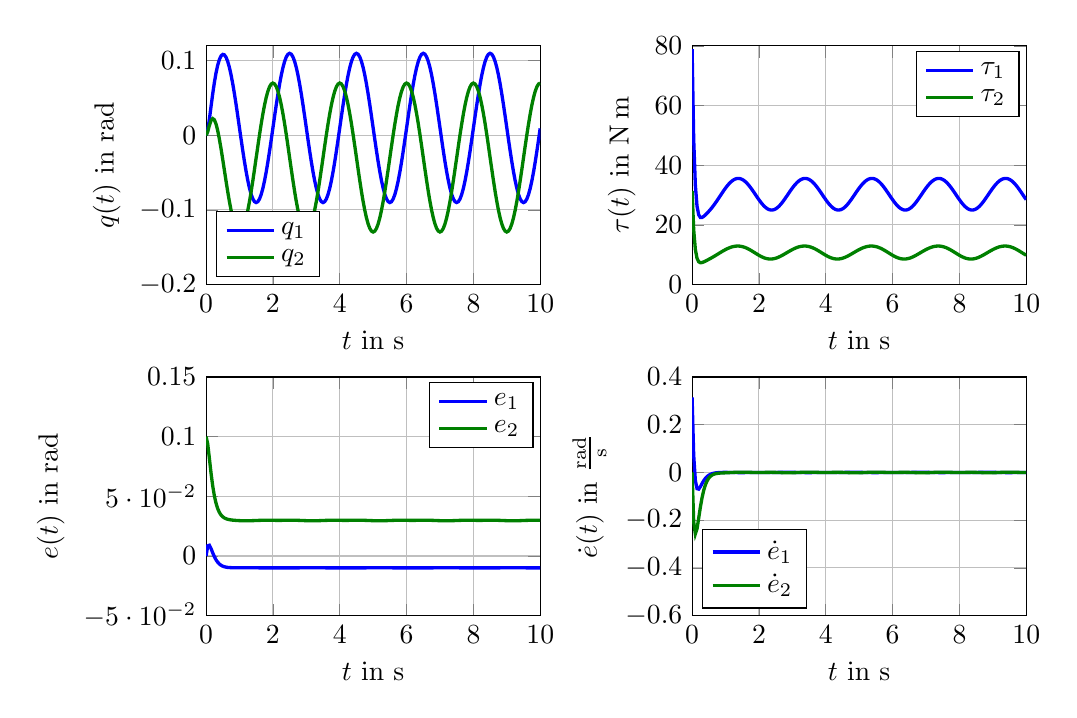
\begin{tikzpicture}

\begin{axis}[%
width=0.35\textwidth,
height=0.25\textwidth,
scale only axis,
xmin=0,
xmax=10,
xlabel={$t$ in $\mathrm{s}$},
xmajorgrids,
ymin=-0.2,
ymax=0.12,
ylabel={$q(t)$ in $\mathrm{rad}$},
ymajorgrids,
name=plot1,
legend style={at={(0.03,0.03)},anchor=south west,draw=black,fill=white,legend cell align=left}
]
\addplot [
color=blue,
solid,
line width=1.2pt
]
table[row sep=crcr]{
0 0\\
0.0478553233355196 0.00649895295253035\\
0.0978553233355196 0.0212690509938064\\
0.14785532333552 0.0385577120396707\\
0.19785532333552 0.0555175440231809\\
0.24785532333552 0.0707823254522751\\
0.29785532333552 0.0837164902437664\\
0.34785532333552 0.0940353675663058\\
0.39785532333552 0.101621113866219\\
0.44785532333552 0.106439414235464\\
0.49785532333552 0.108506145201357\\
0.54785532333552 0.107877281372071\\
0.59785532333552 0.104648343549878\\
0.64785532333552 0.0989566187168452\\
0.69785532333552 0.0909830079010742\\
0.74785532333552 0.0809522092859934\\
0.79785532333552 0.0691308597845268\\
0.84785532333552 0.0558236915754193\\
0.89785532333552 0.041367951143153\\
0.94785532333552 0.0261264019401606\\
0.99785532333552 0.0104792508914508\\
1.04785532333552 -0.00518466573086634\\
1.09785532333551 -0.0204771158262766\\
1.1478553233355 -0.0350198210252502\\
1.1978553233355 -0.0484536383668602\\
1.24785532333549 -0.0604473109356584\\
1.29785532333549 -0.0707055469536055\\
1.34785532333548 -0.0789762121300151\\
1.39785532333548 -0.0850564486533862\\
1.44785532333547 -0.0887975663104525\\
1.49785532333547 -0.0901085865603742\\
1.54785532333546 -0.0889583581264842\\
1.59785532333545 -0.0853762014728175\\
1.64785532333545 -0.0794510778562462\\
1.69785532333544 -0.0713293150367477\\
1.74785532333544 -0.0612109551477067\\
1.79785532333543 -0.0493448202113247\\
1.84785532333543 -0.0360224173977489\\
1.89785532333542 -0.0215708297323846\\
1.94785532333542 -0.0063447588958877\\
1.99785532333541 0.009282094901945\\
2.04785532333541 0.0249261155810446\\
2.0978553233354 0.040203104135948\\
2.14785532333539 0.0547376420774543\\
2.19785532333539 0.0681722629907787\\
2.24785532333538 0.0801762125391584\\
2.29785532333538 0.0904535852339968\\
2.34785532333537 0.0987506392312998\\
2.39785532333537 0.104862107792743\\
2.44785532333536 0.108636347387226\\
2.49785532333536 0.109979187414914\\
2.54785532333535 0.108856375162861\\
2.59785532333534 0.105294541932261\\
2.64785532333534 0.0993806522683567\\
2.69785532333533 0.0912599373990336\\
2.74785532333533 0.0811323552337026\\
2.79785532333532 0.0692476608502496\\
2.84785532333532 0.0558992111912075\\
2.89785532333531 0.0414166636128406\\
2.94785532333531 0.0261577583074948\\
2.9978553233353 0.0104993984208361\\
3.0478553233353 -0.00517174145329799\\
3.09785532333529 -0.0204688376557672\\
3.14785532333528 -0.0350145263127071\\
3.19785532333528 -0.0484502565411202\\
3.24785532333527 -0.060445153839825\\
3.29785532333527 -0.0707041729241086\\
3.34785532333526 -0.0789753381064608\\
3.39785532333526 -0.0850558934678538\\
3.44785532333525 -0.0887972141617673\\
3.49785532333525 -0.090108363526202\\
3.54785532333524 -0.0889582170808056\\
3.59785532333523 -0.0853761124134961\\
3.64785532333523 -0.0794510217098319\\
3.69785532333522 -0.0713292796953298\\
3.74785532333522 -0.0612109329367955\\
3.79785532333521 -0.0493448062741243\\
3.84785532333521 -0.036022408665564\\
3.8978553233352 -0.021570824269463\\
3.9478553233352 -0.00634475548314989\\
3.99785532333519 0.0092820970309787\\
4.04785532333521 0.0249261169075038\\
4.09785532333522 0.0402031049613612\\
4.14785532333524 0.0547376425904975\\
4.19785532333526 0.0681722633093337\\
4.24785532333527 0.080176212736769\\
4.29785532333529 0.0904535853564819\\
4.34785532333531 0.0987506393071682\\
4.39785532333532 0.104862107839711\\
4.44785532333534 0.108636347416291\\
4.49785532333536 0.109979187432896\\
4.54785532333537 0.108856375173983\\
4.59785532333539 0.10529454193914\\
4.64785532333541 0.0993806522726092\\
4.69785532333542 0.0912599374016598\\
4.74785532333544 0.0811323552353204\\
4.79785532333546 0.0692476608512406\\
4.84785532333547 0.0558992111918078\\
4.89785532333549 0.0414166636131962\\
4.94785532333551 0.0261577583076964\\
4.99785532333552 0.0104993984209403\\
5.04785532333554 -0.0051717414532554\\
5.09785532333556 -0.0204688376557632\\
5.14785532333557 -0.0350145263127264\\
5.19785532333559 -0.0484502565411522\\
5.24785532333561 -0.0604451538398621\\
5.29785532333562 -0.0707041729241447\\
5.34785532333564 -0.0789753381064912\\
5.39785532333566 -0.0850558934678744\\
5.44785532333567 -0.0887972141617746\\
5.49785532333569 -0.0901083635261933\\
5.54785532333571 -0.0889582170807785\\
5.59785532333572 -0.085376112413449\\
5.64785532333574 -0.0794510217097637\\
5.69785532333576 -0.0713292796952403\\
5.74785532333577 -0.0612109329366849\\
5.79785532333579 -0.0493448062739937\\
5.84785532333581 -0.0360224086654154\\
5.89785532333582 -0.0215708242692991\\
5.94785532333584 -0.00634475548297399\\
5.99785532333586 0.00928209703116268\\
6.04785532333587 0.0249261169076912\\
6.09785532333589 0.0402031049615463\\
6.14785532333591 0.0547376425906745\\
6.19785532333592 0.0681722633094968\\
6.24785532333594 0.0801762127369134\\
6.29785532333596 0.0904535853566031\\
6.34785532333597 0.0987506393072626\\
6.39785532333599 0.104862107839776\\
6.44785532333601 0.108636347416324\\
6.49785532333602 0.109979187432896\\
6.54785532333604 0.108856375173951\\
6.59785532333606 0.105294541939076\\
6.64785532333607 0.0993806522725148\\
6.69785532333609 0.0912599374015373\\
6.74785532333611 0.0811323552351726\\
6.79785532333612 0.0692476608510713\\
6.84785532333614 0.0558992111916211\\
6.89785532333616 0.0414166636129967\\
6.94785532333617 0.026157758307489\\
6.99785532333619 0.0104993984207302\\
7.04785532333621 -0.00517174145346311\\
7.09785532333622 -0.0204688376559633\\
7.14785532333624 -0.0350145263129141\\
7.19785532333626 -0.0484502565413227\\
7.24785532333627 -0.0604451538400113\\
7.29785532333629 -0.070704172924269\\
7.34785532333631 -0.0789753381065874\\
7.39785532333632 -0.0850558934679403\\
7.44785532333634 -0.0887972141618086\\
7.49785532333636 -0.0901083635261944\\
7.54785532333637 -0.0889582170807469\\
7.59785532333639 -0.0853761124133853\\
7.64785532333641 -0.0794510217096695\\
7.69785532333642 -0.071329279695118\\
7.74785532333644 -0.0612109329365374\\
7.79785532333646 -0.0493448062738248\\
7.84785532333648 -0.0360224086652292\\
7.89785532333649 -0.0215708242691001\\
7.94785532333651 -0.00634475548276707\\
7.99785532333653 0.0092820970313724\\
8.0478553233365 0.0249261169078982\\
8.09785532333647 0.0402031049617441\\
8.14785532333644 0.0547376425908567\\
8.19785532333642 0.0681722633096584\\
8.24785532333639 0.0801762127370507\\
8.29785532333636 0.0904535853567144\\
8.34785532333633 0.0987506393073474\\
8.39785532333631 0.104862107839835\\
8.44785532333628 0.10863634741636\\
8.49785532333625 0.109979187432912\\
8.54785532333622 0.10885637517395\\
8.59785532333619 0.105294541939063\\
8.64785532333617 0.099380652272493\\
8.69785532333614 0.0912599374015116\\
8.74785532333611 0.0811323552351473\\
8.79785532333608 0.0692476608510501\\
8.84785532333606 0.0558992111916071\\
8.89785532333603 0.0414166636129922\\
8.947855323336 0.0261577583074955\\
8.99785532333597 0.0104993984207482\\
9.04785532333594 -0.00517174145343399\\
9.09785532333592 -0.0204688376559245\\
9.14785532333589 -0.0350145263128678\\
9.19785532333586 -0.0484502565412722\\
9.24785532333583 -0.0604451538399602\\
9.29785532333581 -0.0707041729242216\\
9.34785532333578 -0.0789753381065485\\
9.39785532333575 -0.0850558934679147\\
9.44785532333572 -0.0887972141618011\\
9.4978553233357 -0.0901083635262095\\
9.54785532333567 -0.0889582170807886\\
9.59785532333564 -0.0853761124134568\\
9.64785532333561 -0.0794510217097733\\
9.69785532333558 -0.0713292796952552\\
9.74785532333556 -0.0612109329367085\\
9.79785532333553 -0.0493448062740285\\
9.8478553233355 -0.0360224086654631\\
9.89785532333547 -0.0215708242693604\\
9.94785532333545 -0.00634475548304886\\
9.99785532333542 0.00928209703107537\\
};
\addlegendentry{$q_1$};

\addplot [
color=green!50!black,
solid,
line width=1.2pt
]
table[row sep=crcr]{
0 0\\
0.0478553233355196 0.00473598304206479\\
0.0978553233355196 0.0132565650848445\\
0.14785532333552 0.0198538399566668\\
0.19785532333552 0.0224706762800026\\
0.24785532333552 0.020771275933325\\
0.29785532333552 0.0151649894144616\\
0.34785532333552 0.00633581656710969\\
0.39785532333552 -0.00497103577177048\\
0.44785532333552 -0.0180369043369881\\
0.49785532333552 -0.0321994395700148\\
0.54785532333552 -0.0468581502959314\\
0.59785532333552 -0.0614717392239285\\
0.64785532333552 -0.0755542234273369\\
0.69785532333552 -0.0886724137243161\\
0.74785532333552 -0.100445284365203\\
0.79785532333552 -0.110544915778238\\
0.84785532333552 -0.11869841917267\\
0.89785532333552 -0.124690235924725\\
0.94785532333552 -0.128364290200182\\
0.99785532333552 -0.129625586766578\\
1.04785532333552 -0.128440956307256\\
1.09785532333551 -0.124838747259038\\
1.1478553233355 -0.118907344913456\\
1.1978553233355 -0.110792467191373\\
1.24785532333549 -0.100693244508591\\
1.29785532333549 -0.0888571401756885\\
1.34785532333548 -0.0755738085853552\\
1.39785532333548 -0.0611680211840981\\
1.44785532333547 -0.0459918149461158\\
1.49785532333547 -0.0304160352080611\\
1.54785532333546 -0.0148214554297774\\
1.59785532333545 0.000410337472441939\\
1.64785532333545 0.0149061000526603\\
1.69785532333544 0.0283099367274082\\
1.74785532333544 0.0402919544596484\\
1.79785532333543 0.0505563691103565\\
1.84785532333543 0.0588488661202486\\
1.89785532333542 0.064963024514372\\
1.94785532333542 0.0687456265829034\\
1.99785532333541 0.0701006969849113\\
2.04785532333541 0.0689921441860906\\
2.0978553233354 0.0654449127066794\\
2.14785532333539 0.059544594610323\\
2.19785532333539 0.0514354909159927\\
2.24785532333538 0.0413171564380745\\
2.29785532333538 0.0294395037976779\\
2.34785532333537 0.0160965833251568\\
2.39785532333537 0.00161919476790304\\
2.44785532333536 -0.0136334766744015\\
2.49785532333536 -0.0292829748819108\\
2.54785532333535 -0.0449411864026473\\
2.59785532333534 -0.0602201838953595\\
2.64785532333534 -0.0747420235021503\\
2.69785532333533 -0.0881482256307283\\
2.74785532333533 -0.100108685681322\\
2.79785532333532 -0.110329787810781\\
2.84785532333532 -0.118561527625381\\
2.89785532333531 -0.124603485278379\\
2.94785532333531 -0.128309526061246\\
2.9978553233353 -0.129591139688725\\
3.0478553233353 -0.128419361804785\\
3.09785532333529 -0.124825252343101\\
3.14785532333528 -0.1188989360743\\
3.19785532333528 -0.110787241470251\\
3.24785532333527 -0.100690004769838\\
3.29785532333527 -0.0888551359756764\\
3.34785532333526 -0.0755725710494313\\
3.39785532333526 -0.0611672582572561\\
3.44785532333525 -0.0459913452226756\\
3.49785532333525 -0.0304157462974559\\
3.54785532333524 -0.0148212778580069\\
3.59785532333523 0.000410446565703739\\
3.64785532333523 0.0149061670649063\\
3.69785532333522 0.0283099778947484\\
3.74785532333522 0.040291979758028\\
3.79785532333521 0.0505563846649636\\
3.84785532333521 0.0588488756904553\\
3.8978553233352 0.0649630304073095\\
3.9478553233352 0.0687456302147277\\
3.99785532333519 0.0701006992252623\\
4.04785532333521 0.0689921455693482\\
4.09785532333522 0.0654449135614816\\
4.14785532333524 0.0595445951389713\\
4.19785532333526 0.0514354912431486\\
4.24785532333527 0.0413171566406391\\
4.29785532333529 0.0294395039231411\\
4.34785532333531 0.0160965834028755\\
4.39785532333532 0.00161919481604175\\
4.44785532333534 -0.0136334766445945\\
4.49785532333536 -0.0292829748634656\\
4.54785532333537 -0.0449411863912434\\
4.59785532333539 -0.0602201838883177\\
4.64785532333541 -0.0747420234978094\\
4.69785532333542 -0.0881482256280581\\
4.74785532333544 -0.100108685679684\\
4.79785532333546 -0.110329787809778\\
4.84785532333547 -0.118561527624769\\
4.89785532333549 -0.124603485278005\\
4.94785532333551 -0.128309526061015\\
4.99785532333552 -0.129591139688578\\
5.04785532333554 -0.128419361804684\\
5.09785532333556 -0.124825252343025\\
5.14785532333557 -0.118898936074232\\
5.19785532333559 -0.110787241470184\\
5.24785532333561 -0.100690004769766\\
5.29785532333562 -0.0888551359755956\\
5.34785532333564 -0.0755725710493411\\
5.39785532333566 -0.0611672582571564\\
5.44785532333567 -0.0459913452225675\\
5.49785532333569 -0.0304157462973412\\
5.54785532333571 -0.0148212778578882\\
5.59785532333572 0.000410446565823476\\
5.64785532333574 0.0149061670650234\\
5.69785532333576 0.0283099778948592\\
5.74785532333577 0.0402919797581286\\
5.79785532333579 0.0505563846650498\\
5.84785532333581 0.0588488756905233\\
5.89785532333582 0.0649630304073557\\
5.94785532333584 0.0687456302147488\\
5.99785532333586 0.0701006992252558\\
6.04785532333587 0.068992145569312\\
6.09785532333589 0.0654449135614154\\
6.14785532333591 0.0595445951388756\\
6.19785532333592 0.0514354912430253\\
6.24785532333594 0.0413171566404909\\
6.29785532333596 0.0294395039229716\\
6.34785532333597 0.0160965834026887\\
6.39785532333599 0.00161919481584223\\
6.44785532333601 -0.0136334766448018\\
6.49785532333602 -0.0292829748636756\\
6.54785532333604 -0.0449411863914509\\
6.59785532333606 -0.0602201838885176\\
6.64785532333607 -0.0747420234979967\\
6.69785532333609 -0.0881482256282283\\
6.74785532333611 -0.100108685679832\\
6.79785532333612 -0.110329787809902\\
6.84785532333614 -0.118561527624865\\
6.89785532333616 -0.12460348527807\\
6.94785532333617 -0.128309526061049\\
6.99785532333619 -0.129591139688579\\
7.04785532333621 -0.128419361804652\\
7.09785532333622 -0.124825252342961\\
7.14785532333624 -0.118898936074139\\
7.19785532333626 -0.110787241470062\\
7.24785532333627 -0.100690004769619\\
7.29785532333629 -0.0888551359754272\\
7.34785532333631 -0.0755725710491554\\
7.39785532333632 -0.061167258256958\\
7.44785532333634 -0.0459913452223613\\
7.49785532333636 -0.0304157462971321\\
7.54785532333637 -0.0148212778576814\\
7.59785532333639 0.000410446566022849\\
7.64785532333641 0.0149061670652106\\
7.69785532333642 0.0283099778950295\\
7.74785532333644 0.0402919797582778\\
7.79785532333646 0.0505563846651743\\
7.84785532333648 0.0588488756906199\\
7.89785532333649 0.0649630304074221\\
7.94785532333651 0.0687456302147832\\
7.99785532333653 0.0701006992252574\\
8.0478553233365 0.0689921455692811\\
8.09785532333647 0.0654449135613541\\
8.14785532333644 0.059544595138788\\
8.19785532333642 0.0514354912429164\\
8.24785532333639 0.0413171566403664\\
8.29785532333636 0.0294395039228372\\
8.34785532333633 0.0160965834025502\\
8.39785532333631 0.00161919481570491\\
8.44785532333628 -0.0136334766449333\\
8.49785532333625 -0.0292829748637973\\
8.54785532333622 -0.0449411863915598\\
8.59785532333619 -0.0602201838886117\\
8.64785532333617 -0.074742023498075\\
8.69785532333614 -0.0881482256282908\\
8.74785532333611 -0.10010868567988\\
8.79785532333608 -0.110329787809937\\
8.84785532333606 -0.11856152762489\\
8.89785532333603 -0.124603485278088\\
8.947855323336 -0.128309526061064\\
8.99785532333597 -0.129591139688594\\
9.04785532333594 -0.128419361804673\\
9.09785532333592 -0.12482525234299\\
9.14785532333589 -0.118898936074179\\
9.19785532333586 -0.110787241470118\\
9.24785532333583 -0.100690004769692\\
9.29785532333581 -0.0888551359755182\\
9.34785532333578 -0.0755725710492651\\
9.39785532333575 -0.0611672582570856\\
9.44785532333572 -0.0459913452225051\\
9.4978553233357 -0.0304157462972893\\
9.54785532333567 -0.0148212778578481\\
9.59785532333564 0.000410446565851353\\
9.64785532333561 0.0149061670650398\\
9.69785532333558 0.0283099778948655\\
9.74785532333556 0.0402919797581273\\
9.79785532333553 0.050556384665044\\
9.8478553233355 0.0588488756905166\\
9.89785532333547 0.064963030407352\\
9.94785532333545 0.0687456302147525\\
9.99785532333542 0.0701006992252711\\
};
\addlegendentry{$q_2$};

\end{axis}

\begin{axis}[%
width=0.35\textwidth,
height=0.25\textwidth,
scale only axis,
xmin=0,
xmax=10,
xlabel={$t$ in $\mathrm{s}$},
xmajorgrids,
ymin=-0.05,
ymax=0.15,
ylabel={$e(t)$ in $\mathrm{rad}$},
ymajorgrids,
name=plot3,
at=(plot1.below south west),
anchor=above north west,
legend style={draw=black,fill=white,legend cell align=left}
]
\addplot [
color=blue,
solid,
line width=1.2pt
]
table[row sep=crcr]{
0 0\\
0.0478553233355196 0.00847866869014454\\
0.0978553233355196 0.00899115848636926\\
0.14785532333552 0.00623997849272637\\
0.19785532333552 0.00271455974551901\\
0.24785532333552 -0.000549676103330038\\
0.29785532333552 -0.0032126562303469\\
0.34785532333552 -0.00524262045872943\\
0.39785532333552 -0.00672582578450691\\
0.44785532333552 -0.0077782221115931\\
0.49785532333552 -0.00850841502313997\\
0.54785532333552 -0.00900528912993602\\
0.59785532333552 -0.00933664583015521\\
0.64785532333552 -0.0095521058387831\\
0.69785532333552 -0.00968711568829785\\
0.74785532333552 -0.00976671241037889\\
0.79785532333552 -0.00980858143027116\\
0.84785532333552 -0.00982534311495848\\
0.89785532333552 -0.0098261645753498\\
0.94785532333552 -0.00981784073150238\\
0.99785532333552 -0.00980548594390612\\
1.04785532333552 -0.00979295591180718\\
1.09785532333551 -0.00978309365389612\\
1.1478553233355 -0.00977786950714261\\
1.1978553233355 -0.00977846540183429\\
1.24785532333549 -0.00978533841328074\\
1.29785532333549 -0.00979828705980797\\
1.34785532333548 -0.00981653497755587\\
1.39785532333548 -0.00983883942832169\\
1.44785532333547 -0.00986362581341631\\
1.49785532333547 -0.0098891436178425\\
1.54785532333546 -0.00991363411565395\\
1.59785532333545 -0.00993549624691188\\
1.64785532333545 -0.00995343502182593\\
1.69785532333544 -0.0099665771760427\\
1.74785532333544 -0.00997454172792589\\
1.79785532333543 -0.00997745814295307\\
1.84785532333543 -0.00997593106273786\\
1.89785532333542 -0.00997095683544795\\
1.94785532333542 -0.00996380231280291\\
1.99785532333541 -0.00995585984952415\\
2.04785532333541 -0.00994849393840524\\
2.0978553233354 -0.00994289465580821\\
2.14785532333539 -0.00993995154509247\\
2.19785532333539 -0.0099401592221122\\
2.24785532333538 -0.00994356319024389\\
2.29785532333538 -0.00994975122060375\\
2.34785532333537 -0.00995789212374477\\
2.39785532333537 -0.00996681971104631\\
2.44785532333536 -0.00997515526336248\\
2.49785532333536 -0.00998145723669762\\
2.54785532333535 -0.00998438292071745\\
2.59785532333534 -0.00998284421252163\\
2.64785532333534 -0.00997613939026916\\
2.69785532333533 -0.00996404518622314\\
2.74785532333533 -0.00994685835804582\\
2.79785532333532 -0.00992538249594389\\
2.84785532333532 -0.00990086273069005\\
2.89785532333531 -0.00987487704497519\\
2.94785532333531 -0.0098491970987702\\
2.9978553233353 -0.00982563347322229\\
3.0478553233353 -0.00980588018930713\\
3.09785532333529 -0.00979137182433966\\
3.14785532333528 -0.00978316421962386\\
3.19785532333528 -0.00978184722751806\\
3.24785532333527 -0.00978749550906481\\
3.29785532333527 -0.0097996610892639\\
3.34785532333526 -0.00981740900107837\\
3.39785532333526 -0.00983939461383229\\
3.44785532333525 -0.00986397796209024\\
3.49785532333525 -0.00988936665201427\\
3.54785532333524 -0.0099137751613429\\
3.59785532333523 -0.00993558530625414\\
3.64785532333523 -0.0099534911682712\\
3.69785532333522 -0.00996661251750082\\
3.74785532333522 -0.00997456393888566\\
3.79785532333521 -0.00997747208020918\\
3.84785532333521 -0.0099759397949843\\
3.8978553233352 -0.0099709622984353\\
3.9478553233352 -0.00996380572560892\\
3.99785532333519 -0.00995586197862696\\
4.04785532333521 -0.00994849526492641\\
4.09785532333522 -0.0099428954812745\\
4.14785532333524 -0.00993995205817923\\
4.19785532333526 -0.00994015954070122\\
4.24785532333527 -0.00994356338787931\\
4.29785532333529 -0.00994975134310545\\
4.34785532333531 -0.00995789219962272\\
4.39785532333532 -0.00996681975801875\\
4.44785532333534 -0.00997515529242866\\
4.49785532333536 -0.00998145725467905\\
4.54785532333537 -0.00998438293184105\\
4.59785532333539 -0.00998284421940471\\
4.64785532333541 -0.00997613939453111\\
4.69785532333542 -0.00996404518886564\\
4.74785532333544 -0.00994685835968812\\
4.79785532333546 -0.00992538249696875\\
4.84785532333547 -0.00990086273133382\\
4.89785532333549 -0.00987487704538385\\
4.94785532333551 -0.0098491970990338\\
4.99785532333552 -0.00982563347339646\\
5.04785532333554 -0.00980588018942575\\
5.09785532333556 -0.00979137182442355\\
5.14785532333557 -0.00978316421968585\\
5.19785532333559 -0.00978184722756555\\
5.24785532333561 -0.00978749550910245\\
5.29785532333562 -0.00979966108929405\\
5.34785532333564 -0.00981740900110264\\
5.39785532333566 -0.0098393946138513\\
5.44785532333567 -0.00986397796210456\\
5.49785532333569 -0.00988936665202393\\
5.54785532333571 -0.00991377516134803\\
5.59785532333572 -0.00993558530625482\\
5.64785532333574 -0.00995349116826733\\
5.69785532333576 -0.00996661251749284\\
5.74785532333577 -0.00997456393887365\\
5.79785532333579 -0.00997747208019372\\
5.84785532333581 -0.00997593979496535\\
5.89785532333582 -0.00997096229841377\\
5.94785532333584 -0.00996380572558506\\
5.99785532333586 -0.00995586197860172\\
6.04785532333587 -0.00994849526490622\\
6.09785532333589 -0.00994289548125972\\
6.14785532333591 -0.00993995205816852\\
6.19785532333592 -0.00994015954069385\\
6.24785532333594 -0.00994356338787424\\
6.29785532333596 -0.00994975134310221\\
6.34785532333597 -0.00995789219962055\\
6.39785532333599 -0.0099668197580174\\
6.44785532333601 -0.00997515529242775\\
6.49785532333602 -0.00998145725467837\\
6.54785532333604 -0.00998438293184054\\
6.59785532333606 -0.00998284421940417\\
6.64785532333607 -0.00997613939453068\\
6.69785532333609 -0.00996404518886519\\
6.74785532333611 -0.0099468583596877\\
6.79785532333612 -0.00992538249696849\\
6.84785532333614 -0.00990086273133343\\
6.89785532333616 -0.0098748770453836\\
6.94785532333617 -0.00984919709903339\\
6.99785532333619 -0.00982563347339627\\
7.04785532333621 -0.00980588018942544\\
7.09785532333622 -0.0097913718244235\\
7.14785532333624 -0.00978316421968556\\
7.19785532333626 -0.00978184722756571\\
7.24785532333627 -0.00978749550910244\\
7.29785532333629 -0.00979966108929432\\
7.34785532333631 -0.00981740900110278\\
7.39785532333632 -0.00983939461385165\\
7.44785532333634 -0.00986397796210479\\
7.49785532333636 -0.00988936665202425\\
7.54785532333637 -0.00991377516134828\\
7.59785532333639 -0.00993558530625499\\
7.64785532333641 -0.00995349116826766\\
7.69785532333642 -0.00996661251749292\\
7.74785532333644 -0.00997456393887389\\
7.79785532333646 -0.00997747208019362\\
7.84785532333648 -0.00997593979496549\\
7.89785532333649 -0.00997096229841358\\
7.94785532333651 -0.00996380572558519\\
7.99785532333653 -0.0099558619786015\\
8.0478553233365 -0.00994849526491901\\
8.09785532333647 -0.00994289548128345\\
8.14785532333644 -0.00993995205820019\\
8.19785532333642 -0.00994015954072978\\
8.24785532333639 -0.00994356338791146\\
8.29785532333636 -0.00994975134313826\\
8.34785532333633 -0.00995789219965358\\
8.39785532333631 -0.00996681975804557\\
8.44785532333628 -0.00997515529244979\\
8.49785532333625 -0.00998145725469345\\
8.54785532333622 -0.00998438293184786\\
8.59785532333619 -0.00998284421940344\\
8.64785532333617 -0.00997613939452191\\
8.69785532333614 -0.00996404518884841\\
8.74785532333611 -0.00994685835966316\\
8.79785532333608 -0.0099253824969367\\
8.84785532333606 -0.00990086273129572\\
8.89785532333603 -0.0098748770453403\\
8.947855323336 -0.00984919709898588\\
8.99785532333597 -0.00982563347334534\\
9.04785532333594 -0.00980588018937304\\
9.09785532333592 -0.00979137182437021\\
9.14785532333589 -0.00978316421963303\\
9.19785532333586 -0.0097818472275149\\
9.24785532333583 -0.00978749550905517\\
9.29785532333581 -0.00979966108925125\\
9.34785532333578 -0.00981740900106519\\
9.39785532333575 -0.00983939461382025\\
9.44785532333572 -0.00986397796208059\\
9.4978553233357 -0.00988936665200767\\
9.54785532333567 -0.00991377516133983\\
9.59785532333564 -0.00993558530625498\\
9.64785532333561 -0.00995349116827578\\
9.69785532333558 -0.00996661251750937\\
9.74785532333556 -0.00997456393889799\\
9.79785532333553 -0.00997747208022506\\
9.8478553233355 -0.00997593979500293\\
9.89785532333547 -0.00997096229845668\\
9.94785532333545 -0.00996380572563256\\
9.99785532333542 -0.0099558619786523\\
};
\addlegendentry{$e_1$};

\addplot [
color=green!50!black,
solid,
line width=1.2pt
]
table[row sep=crcr]{
0 0.1\\
0.0478553233355196 0.0941360092000706\\
0.0978553233355196 0.0820551326348787\\
0.14785532333552 0.0695506729213953\\
0.19785532333552 0.0588252159327738\\
0.24785532333552 0.0504142209422896\\
0.29785532333552 0.0441572889397941\\
0.34785532333552 0.0396625318933512\\
0.39785532333552 0.0365128223395738\\
0.44785532333552 0.0343454655456465\\
0.49785532333552 0.0328732045175596\\
0.54785532333552 0.0318805286532564\\
0.59785532333552 0.0312115297437526\\
0.64785532333552 0.0307565328949397\\
0.69785532333552 0.0304403099556161\\
0.74785532333552 0.0302126350162582\\
0.79785532333552 0.0300410817648189\\
0.84785532333552 0.0299056720650939\\
0.89785532333552 0.0297949478430124\\
0.94785532333552 0.0297030980763109\\
0.99785532333552 0.0296278565883615\\
1.04785532333552 0.0295689640651206\\
1.09785532333551 0.029527049539314\\
1.1478553233355 0.0295028320353922\\
1.1978553233355 0.0294965749785929\\
1.24785532333549 0.0295077476329703\\
1.29785532333549 0.0295348618214246\\
1.34785532333548 0.0295754601248837\\
1.39785532333548 0.0296262346162819\\
1.44785532333547 0.0296832537374422\\
1.49785532333547 0.0297422702604992\\
1.54785532333546 0.0297990770724338\\
1.59785532333545 0.0298498720077143\\
1.64785532333545 0.029891590479717\\
1.69785532333544 0.0299221670412722\\
1.74785532333544 0.0299406948892784\\
1.79785532333543 0.0299474649030468\\
1.84785532333543 0.0299438809873144\\
1.89785532333542 0.0299322635673305\\
1.94785532333542 0.0299155655409626\\
1.99785532333541 0.0298970331933053\\
2.04785532333541 0.0298798480560502\\
2.0978553233354 0.0298667850130552\\
2.14785532333539 0.0298599182677568\\
2.19785532333539 0.0298604012968077\\
2.24785532333538 0.0298683404375702\\
2.29785532333538 0.0298827745566137\\
2.34785532333537 0.0299017651353453\\
2.39785532333537 0.0299225917999459\\
2.44785532333536 0.0299420378831092\\
2.49785532333536 0.0299567398295072\\
2.54785532333535 0.029963564760025\\
2.59785532333534 0.0299599744152362\\
2.64785532333534 0.0299443329698039\\
2.69785532333533 0.029916121862076\\
2.74785532333533 0.0298760363324195\\
2.79785532333532 0.0298259537973978\\
2.84785532333532 0.0297687805178343\\
2.89785532333531 0.0297081971966876\\
2.94785532333531 0.029648333937386\\
2.9978553233353 0.0295934095105086\\
3.0478553233353 0.0295473695626386\\
3.09785532333529 0.0295135546233562\\
3.14785532333528 0.0294944231962047\\
3.19785532333528 0.0294913492574307\\
3.24785532333527 0.0295045078941693\\
3.29785532333527 0.0295328576213568\\
3.34785532333526 0.0295742225888985\\
3.39785532333526 0.0296254716893743\\
3.44785532333525 0.0296827840139338\\
3.49785532333525 0.0297419813498249\\
3.54785532333524 0.029798899500595\\
3.59785532333523 0.0298497629143867\\
3.64785532333523 0.0298915234674091\\
3.69785532333522 0.0299221258738758\\
3.74785532333522 0.0299406695908495\\
3.79785532333521 0.0299474493483986\\
3.84785532333521 0.0299438714170759\\
3.8978553233352 0.0299322576743711\\
3.9478553233352 0.029915561909127\\
3.99785532333519 0.0298970309529538\\
4.04785532333521 0.0298798466728019\\
4.09785532333522 0.0298667841582698\\
4.14785532333524 0.0298599177391303\\
4.19785532333526 0.0298604009696761\\
4.24785532333527 0.0298683402350301\\
4.29785532333529 0.0298827744311731\\
4.34785532333531 0.029901765057645\\
4.39785532333532 0.0299225917518203\\
4.44785532333534 0.0299420378533088\\
4.49785532333536 0.0299567398110618\\
4.54785532333537 0.0299635647486141\\
4.59785532333539 0.029959974408181\\
4.64785532333541 0.0299443329654441\\
4.69785532333542 0.0299161218593829\\
4.74785532333544 0.0298760363307564\\
4.79785532333546 0.0298259537963706\\
4.84785532333547 0.0297687805171998\\
4.89785532333549 0.0297081971962959\\
4.94785532333551 0.0296483339371446\\
4.99785532333552 0.0295934095103608\\
5.04785532333554 0.0295473695625497\\
5.09785532333556 0.0295135546233048\\
5.14785532333557 0.0294944231961779\\
5.19785532333559 0.0294913492574203\\
5.24785532333561 0.0295045078941705\\
5.29785532333562 0.0295328576213659\\
5.34785532333564 0.0295742225889138\\
5.39785532333566 0.0296254716893938\\
5.44785532333567 0.0296827840139568\\
5.49785532333569 0.0297419813498497\\
5.54785532333571 0.0297988995006213\\
5.59785532333572 0.0298497629144132\\
5.64785532333574 0.0298915234674357\\
5.69785532333576 0.0299221258739012\\
5.74785532333577 0.0299406695908733\\
5.79785532333579 0.02994744934842\\
5.84785532333581 0.0299438714170946\\
5.89785532333582 0.0299322576743865\\
5.94785532333584 0.0299155619091389\\
5.99785532333586 0.0298970309529618\\
6.04785532333587 0.0298798466728067\\
6.09785532333589 0.0298667841582726\\
6.14785532333591 0.029859917739132\\
6.19785532333592 0.0298604009696773\\
6.24785532333594 0.0298683402350308\\
6.29785532333596 0.0298827744311737\\
6.34785532333597 0.0299017650576456\\
6.39785532333599 0.0299225917518209\\
6.44785532333601 0.0299420378533092\\
6.49785532333602 0.0299567398110623\\
6.54785532333604 0.0299635647486142\\
6.59785532333606 0.0299599744081811\\
6.64785532333607 0.0299443329654439\\
6.69785532333609 0.0299161218593827\\
6.74785532333611 0.0298760363307559\\
6.79785532333612 0.0298259537963699\\
6.84785532333614 0.0297687805171991\\
6.89785532333616 0.0297081971962951\\
6.94785532333617 0.029648333937144\\
6.99785532333619 0.0295934095103605\\
7.04785532333621 0.0295473695625494\\
7.09785532333622 0.0295135546233048\\
7.14785532333624 0.0294944231961779\\
7.19785532333626 0.0294913492574206\\
7.24785532333627 0.0295045078941707\\
7.29785532333629 0.0295328576213665\\
7.34785532333631 0.0295742225889142\\
7.39785532333632 0.0296254716893946\\
7.44785532333634 0.0296827840139573\\
7.49785532333636 0.0297419813498506\\
7.54785532333637 0.0297988995006218\\
7.59785532333639 0.0298497629144139\\
7.64785532333641 0.0298915234674359\\
7.69785532333642 0.0299221258739016\\
7.74785532333644 0.0299406695908733\\
7.79785532333646 0.0299474493484201\\
7.84785532333648 0.0299438714170944\\
7.89785532333649 0.0299322576743864\\
7.94785532333651 0.0299155619091386\\
7.99785532333653 0.0298970309529616\\
8.0478553233365 0.0298798466728082\\
8.09785532333647 0.0298667841582787\\
8.14785532333644 0.0298599177391442\\
8.19785532333642 0.0298604009696962\\
8.24785532333639 0.0298683402350566\\
8.29785532333636 0.029882774431206\\
8.34785532333633 0.0299017650576841\\
8.39785532333631 0.0299225917518645\\
8.44785532333628 0.0299420378533569\\
8.49785532333625 0.0299567398111129\\
8.54785532333622 0.0299635647486669\\
8.59785532333619 0.0299599744082342\\
8.64785532333617 0.0299443329654962\\
8.69785532333614 0.0299161218594329\\
8.74785532333611 0.029876036330803\\
8.79785532333608 0.0298259537964126\\
8.84785532333606 0.0297687805172362\\
8.89785532333603 0.0297081971963259\\
8.947855323336 0.0296483339371677\\
8.99785532333597 0.0295934095103764\\
9.04785532333594 0.0295473695625574\\
9.09785532333592 0.0295135546233043\\
9.14785532333589 0.0294944231961692\\
9.19785532333586 0.0294913492574037\\
9.24785532333583 0.0295045078941463\\
9.29785532333581 0.0295328576213349\\
9.34785532333578 0.0295742225888763\\
9.39785532333575 0.029625471689351\\
9.44785532333572 0.0296827840139097\\
9.4978553233357 0.0297419813497996\\
9.54785532333567 0.0297988995005689\\
9.59785532333564 0.0298497629143602\\
9.64785532333561 0.0298915234673834\\
9.69785532333558 0.0299221258738509\\
9.74785532333556 0.029940669590826\\
9.79785532333553 0.0299474493483771\\
9.8478553233355 0.0299438714170572\\
9.89785532333547 0.0299322576743555\\
9.94785532333545 0.029915561909115\\
9.99785532333542 0.0298970309529456\\
};
\addlegendentry{$e_2$};

\end{axis}

\begin{axis}[%
width=0.35\textwidth,
height=0.25\textwidth,
scale only axis,
xmin=0,
xmax=10,
xlabel={$t$ in $\mathrm{s}$},
xmajorgrids,
ymin=-0.6,
ymax=0.4,
ylabel={$\dot{e}(t)$ in $\mathrm{\frac{rad}{s}}$},
ymajorgrids,
name=plot2,
at=(plot3.right of south east),
anchor=left of south west,
legend style={at={(0.03,0.03)},anchor=south west,draw=black,fill=white,legend cell align=left}
]
\addplot [
color=blue,
solid,
line width=1.2pt
]
table[row sep=crcr]{
0 0.314159265358979\\
0.0478553233355196 0.0718837891095546\\
0.0978553233355196 -0.0341932557434544\\
0.14785532333552 -0.0678915261819828\\
0.19785532333552 -0.0697454925777605\\
0.24785532333552 -0.0596034570768608\\
0.29785532333552 -0.0466249001669294\\
0.34785532333552 -0.0346141194711415\\
0.39785532333552 -0.0248141748937048\\
0.44785532333552 -0.0173336378463463\\
0.49785532333552 -0.0118486580541545\\
0.54785532333552 -0.00792899154811836\\
0.59785532333552 -0.00517465108612429\\
0.64785532333552 -0.00326132253245781\\
0.69785532333552 -0.00194489596953049\\
0.74785532333552 -0.00105006374654298\\
0.79785532333552 -0.000454723378053079\\
0.84785532333552 -7.52364729759147e-05\\
0.89785532333552 0.000145660314398111\\
0.94785532333552 0.000247989695558393\\
0.99785532333552 0.000261025917154933\\
1.04785532333552 0.000207650942373516\\
1.09785532333551 0.000107084891008025\\
1.1478553233355 -2.35702417328842e-05\\
1.1978553233355 -0.000168625138521339\\
1.24785532333549 -0.000313670893750118\\
1.29785532333549 -0.0004458195028825\\
1.34785532333548 -0.000554159787384406\\
1.39785532333548 -0.000630295853299614\\
1.44785532333547 -0.000668847905764644\\
1.49785532333547 -0.000667805629901617\\
1.54785532333546 -0.000628641644127036\\
1.59785532333545 -0.000556122880862459\\
1.64785532333545 -0.000457801683535652\\
1.69785532333544 -0.000343220063469207\\
1.74785532333544 -0.000222909400475979\\
1.79785532333543 -0.000107302514577634\\
1.84785532333543 -5.68759267760566e-06\\
1.89785532333542 7.46775926209753e-05\\
1.94785532333542 0.00012920233864866\\
1.99785532333541 0.000156300636287243\\
2.04785532333541 0.000157418312608182\\
2.0978553233354 0.000136769123543601\\
2.14785532333539 0.000100819806664987\\
2.19785532333539 5.75758939073689e-05\\
2.24785532333538 1.57272247674478e-05\\
2.29785532333538 -1.62809716989787e-05\\
2.34785532333537 -3.11763933157627e-05\\
2.39785532333537 -2.3702003664236e-05\\
2.44785532333536 8.71978109880794e-06\\
2.49785532333536 6.55896317961241e-05\\
2.54785532333535 0.000143269154668113\\
2.59785532333534 0.000235284529752536\\
2.64785532333534 0.000332974974690287\\
2.69785532333533 0.000426411084442746\\
2.74785532333533 0.000505465036589714\\
2.79785532333532 0.000560893654472983\\
2.84785532333532 0.000585300969673852\\
2.89785532333531 0.000573875790768563\\
2.94785532333531 0.000524842256871272\\
2.9978553233353 0.000439605616235461\\
3.0478553233353 0.000322611646107085\\
3.09785532333529 0.000180960964265453\\
3.14785532333528 2.38289312132212e-05\\
3.19785532333528 -0.00013825808878265\\
3.24785532333527 -0.000294242702581132\\
3.29785532333527 -0.000433406485628202\\
3.34785532333526 -0.000546239476079735\\
3.39785532333526 -0.00062524898467875\\
3.44785532333525 -0.000665636430952764\\
3.49785532333525 -0.000665764957890688\\
3.54785532333524 -0.000627346824557576\\
3.59785532333523 -0.000555302541135588\\
3.64785532333523 -0.000457282752714949\\
3.69785532333522 -0.000342892313697524\\
3.74785532333522 -0.000222702727912638\\
3.79785532333521 -0.000107172399960442\\
3.84785532333521 -5.60580780439857e-06\\
3.8978553233352 7.47289177310262e-05\\
3.9478553233352 0.000129234498103425\\
3.99785532333519 0.000156320756218298\\
4.04785532333521 0.000157430881733145\\
4.09785532333522 0.000136776964524743\\
4.14785532333524 0.000100824691538937\\
4.19785532333526 5.75789333145948e-05\\
4.24785532333527 1.5729113697488e-05\\
4.29785532333529 -1.62797990257146e-05\\
4.34785532333531 -3.11756660067997e-05\\
4.39785532333532 -2.37015529591655e-05\\
4.44785532333534 8.7200601935622e-06\\
4.49785532333536 6.55898045227405e-05\\
4.54785532333537 0.000143269261520529\\
4.59785532333539 0.000235284595838561\\
4.64785532333541 0.000332975015564702\\
4.69785532333542 0.000426411109734071\\
4.74785532333544 0.000505465052254017\\
4.79785532333546 0.000560893664192985\\
4.84785532333547 0.00058530097572479\\
4.89785532333549 0.000573875794557421\\
4.94785532333551 0.000524842259265246\\
4.99785532333552 0.000439605617770511\\
5.04785532333554 0.000322611647112891\\
5.09785532333556 0.00018096096494441\\
5.14785532333557 2.38289316898399e-05\\
5.19785532333559 -0.000138258088433374\\
5.24785532333561 -0.000294242702313097\\
5.29785532333562 -0.000433406485414678\\
5.34785532333564 -0.000546239475905846\\
5.39785532333566 -0.000625248984535129\\
5.44785532333567 -0.00066563643083515\\
5.49785532333569 -0.000665764957796618\\
5.54785532333571 -0.000627346824487222\\
5.59785532333572 -0.000555302541087752\\
5.64785532333574 -0.000457282752690358\\
5.69785532333576 -0.000342892313695442\\
5.74785532333577 -0.000222702727933538\\
5.79785532333579 -0.000107172400002853\\
5.84785532333581 -5.60580786757026e-06\\
5.89785532333582 7.47289176492028e-05\\
5.94785532333584 0.000129234498004616\\
5.99785532333586 0.000156320756104944\\
6.04785532333587 0.000157430881620568\\
6.09785532333589 0.00013677696442943\\
6.14785532333591 0.00010082469146494\\
6.19785532333592 5.75789332594168e-05\\
6.24785532333594 1.57291136581028e-05\\
6.29785532333596 -1.62797990534702e-05\\
6.34785532333597 -3.11756660252571e-05\\
6.39785532333599 -2.37015529717666e-05\\
6.44785532333601 8.72006018640126e-06\\
6.49785532333602 6.55898045179124e-05\\
6.54785532333604 0.000143269261518253\\
6.59785532333606 0.000235284595837076\\
6.64785532333607 0.000332975015564424\\
6.69785532333609 0.000426411109734071\\
6.74785532333611 0.000505465052254489\\
6.79785532333612 0.00056089366419293\\
6.84785532333614 0.000585300975724568\\
6.89785532333616 0.000573875794556977\\
6.94785532333617 0.000524842259264302\\
6.99785532333619 0.000439605617769123\\
7.04785532333621 0.00032261164711106\\
7.09785532333622 0.000180960964942467\\
7.14785532333624 2.3828931687897e-05\\
7.19785532333626 -0.000138258088435372\\
7.24785532333627 -0.00029424270231479\\
7.29785532333629 -0.000433406485416815\\
7.34785532333631 -0.00054623947590679\\
7.39785532333632 -0.000625248984536642\\
7.44785532333634 -0.000665636430835254\\
7.49785532333636 -0.000665764957797327\\
7.54785532333637 -0.000627346824486376\\
7.59785532333639 -0.000555302541087627\\
7.64785532333641 -0.00045728275268872\\
7.69785532333642 -0.000342892313694498\\
7.74785532333644 -0.000222702727931678\\
7.79785532333646 -0.000107172400001743\\
7.84785532333648 -5.60580786618248e-06\\
7.89785532333649 7.47289176499244e-05\\
7.94785532333651 0.000129234498005171\\
7.99785532333653 0.000156320756105166\\
8.0478553233365 0.000157430881646325\\
8.09785532333647 0.000136776964507201\\
8.14785532333644 0.000100824691594337\\
8.19785532333642 5.75789334293364e-05\\
8.24785532333639 1.57291138545013e-05\\
8.29785532333636 -1.62797988441377e-05\\
8.34785532333633 -3.11756658163687e-05\\
8.39785532333631 -2.37015527745355e-05\\
8.44785532333628 8.72006036291978e-06\\
8.49785532333625 6.55898046675188e-05\\
8.54785532333622 0.000143269261634001\\
8.59785532333619 0.00023528459591439\\
8.64785532333617 0.000332975015600451\\
8.69785532333614 0.000426411109728131\\
8.74785532333611 0.000505465052205473\\
8.79785532333608 0.000560893664101614\\
8.84785532333606 0.000585300975593728\\
8.89785532333603 0.000573875794389167\\
8.947855323336 0.000524842259064073\\
8.99785532333597 0.000439605617541194\\
9.04785532333594 0.000322611646861037\\
9.09785532333592 0.00018096096467668\\
9.14785532333589 2.38289314121731e-05\\
9.19785532333586 -0.000138258088712984\\
9.24785532333583 -0.000294242702588654\\
9.29785532333581 -0.000433406485679494\\
9.34785532333578 -0.000546239476152705\\
9.39785532333575 -0.00062524898475802\\
9.44785532333572 -0.000665636431028835\\
9.4978553233357 -0.000665764957957322\\
9.54785532333567 -0.000627346824609937\\
9.59785532333564 -0.000555302541169492\\
9.64785532333561 -0.000457282752728994\\
9.69785532333558 -0.000342892313691112\\
9.74785532333556 -0.000222702727885493\\
9.79785532333553 -0.000107172399912592\\
9.8478553233355 -5.6058077373411e-06\\
9.89785532333547 7.47289178161248e-05\\
9.94785532333545 0.000129234498204345\\
9.99785532333542 0.000156320756332484\\
};
\addlegendentry{$\dot{e}_1$};

\addplot [
color=green!50!black,
solid,
line width=1.2pt
]
table[row sep=crcr]{
0 -0\\
0.0478553233355196 -0.207425188194469\\
0.0978553233355196 -0.257312115559111\\
0.14785532333552 -0.23583367721319\\
0.19785532333552 -0.191426166825414\\
0.24785532333552 -0.145444851658825\\
0.29785532333552 -0.105990097095687\\
0.34785532333552 -0.0750434435695258\\
0.39785532333552 -0.0520337183946901\\
0.44785532333552 -0.0355385293158254\\
0.49785532333552 -0.0240383244898608\\
0.54785532333552 -0.0162069234848292\\
0.59785532333552 -0.0109878726678331\\
0.64785532333552 -0.00758115404752174\\
0.69785532333552 -0.00539966016283128\\
0.74785532333552 -0.00402173706960507\\
0.79785532333552 -0.00314986360535471\\
0.84785532333552 -0.0025780238569425\\
0.89785532333552 -0.002167202787491\\
0.94785532333552 -0.00182741586998236\\
0.99785532333552 -0.00150459964634737\\
1.04785532333552 -0.00117095596319484\\
1.09785532333551 -0.000817683640505745\\
1.1478553233355 -0.000449335368432779\\
1.1978553233355 -7.92743116882766e-05\\
1.24785532333549 0.000274119045646393\\
1.29785532333549 0.000590704972182832\\
1.34785532333548 0.000851412767232496\\
1.39785532333548 0.00104065028201222\\
1.44785532333547 0.00114822873438741\\
1.49785532333547 0.00117068712199431\\
1.54785532333546 0.00111189070103129\\
1.59785532333545 0.000982815868092957\\
1.64785532333545 0.000800515662448764\\
1.69785532333544 0.000586368381062963\\
1.74785532333544 0.000363818665184201\\
1.79785532333543 0.000155896794646004\\
1.84785532333543 -1.71723020752357e-05\\
1.89785532333542 -0.000139988005411262\\
1.94785532333542 -0.000203411044690002\\
1.99785532333541 -0.000205302436322892\\
2.04785532333541 -0.000150539734509812\\
2.0978553233354 -5.03586196336503e-05\\
2.14785532333539 7.88847925113356e-05\\
2.19785532333539 0.000217409442713201\\
2.24785532333538 0.000344025976183965\\
2.29785532333538 0.000438322655979539\\
2.34785532333537 0.00048284721131886\\
2.39785532333537 0.000465086123241365\\
2.44785532333536 0.000379025401549438\\
2.49785532333536 0.000226083872721217\\
2.54785532333535 1.5256069438252e-05\\
2.59785532333534 -0.000237608607562667\\
2.64785532333534 -0.000511341946223931\\
2.69785532333533 -0.000781631450839704\\
2.74785532333533 -0.00102355427300094\\
2.79785532333532 -0.00121414183007501\\
2.84785532333532 -0.00133466039291949\\
2.89785532333531 -0.00137236224314397\\
2.94785532333531 -0.00132156344936061\\
2.9978553233353 -0.00118400943554127\\
3.0478553233353 -0.000968574606231919\\
3.09785532333529 -0.000690394867775973\\
3.14785532333528 -0.000369552094834136\\
3.19785532333528 -2.94273993677596e-05\\
3.24785532333527 0.000305169897349772\\
3.29785532333527 0.000609994656567414\\
3.34785532333526 0.000863366543775723\\
3.39785532333526 0.00104804175392076\\
3.44785532333525 0.00115279042076499\\
3.49785532333525 0.00117349783566401\\
3.54785532333524 0.00111362026413936\\
3.59785532333523 0.000983879077712024\\
3.64785532333523 0.000801168789705042\\
3.69785532333522 0.00058676943589081\\
3.74785532333522 0.000364064906604289\\
3.79785532333521 0.000156048006208082\\
3.84785532333521 -1.70794100513016e-05\\
3.8978553233352 -0.000139930906238719\\
3.9478553233352 -0.000203375920118924\\
3.99785532333519 -0.00020528081033546\\
4.04785532333521 -0.000150526406690533\\
4.09785532333522 -5.03503976491959e-05\\
4.14785532333524 7.88898697226814e-05\\
4.19785532333526 0.000217412580930304\\
4.24785532333527 0.000344027917563022\\
4.29785532333529 0.000438323857834766\\
4.34785532333531 0.000482847955775467\\
4.39785532333532 0.000465086584551799\\
4.44785532333534 0.000379025687459178\\
4.49785532333536 0.000226084049920194\\
4.54785532333537 1.52561792409744e-05\\
4.59785532333539 -0.000237608539544965\\
4.64785532333541 -0.000511341904107065\\
4.69785532333542 -0.000781631424771112\\
4.74785532333544 -0.00102355425687004\\
4.79785532333546 -0.00121414182009372\\
4.84785532333547 -0.00133466038674065\\
4.89785532333549 -0.0013723622393169\\
4.94785532333551 -0.00132156344698812\\
4.99785532333552 -0.00118400943407019\\
5.04785532333554 -0.00096857460532121\\
5.09785532333556 -0.000690394867217531\\
5.14785532333557 -0.000369552094499154\\
5.19785532333559 -2.94273991783556e-05\\
5.24785532333561 0.000305169897442975\\
5.29785532333562 0.000609994656594171\\
5.34785532333564 0.000863366543753907\\
5.39785532333566 0.00104804175386336\\
5.44785532333567 0.00115279042068017\\
5.49785532333569 0.00117349783555892\\
5.54785532333571 0.00111362026401896\\
5.59785532333572 0.000983879077580962\\
5.64785532333574 0.000801168789567486\\
5.69785532333576 0.000586769435750367\\
5.74785532333577 0.000364064906465622\\
5.79785532333579 0.000156048006074189\\
5.84785532333581 -1.70794101758132e-05\\
5.89785532333582 -0.000139930906352184\\
5.94785532333584 -0.000203375920216853\\
5.99785532333586 -0.000205280810416329\\
6.04785532333587 -0.000150526406739002\\
6.09785532333589 -5.03503976778535e-05\\
6.14785532333591 7.8889869706722e-05\\
6.19785532333592 0.000217412580921061\\
6.24785532333594 0.000344027917558193\\
6.29785532333596 0.000438323857831546\\
6.34785532333597 0.000482847955773469\\
6.39785532333599 0.000465086584549634\\
6.44785532333601 0.000379025687456624\\
6.49785532333602 0.000226084049917308\\
6.54785532333604 1.52561792373662e-05\\
6.59785532333606 -0.000237608539548906\\
6.64785532333607 -0.000511341904111173\\
6.69785532333609 -0.000781631424774609\\
6.74785532333611 -0.00102355425687356\\
6.79785532333612 -0.0012141418200961\\
6.84785532333614 -0.00133466038674179\\
6.89785532333616 -0.00137236223931735\\
6.94785532333617 -0.00132156344698679\\
6.99785532333619 -0.00118400943406885\\
7.04785532333621 -0.00096857460531867\\
7.09785532333622 -0.000690394867214519\\
7.14785532333624 -0.000369552094495545\\
7.19785532333626 -2.94273991746086e-05\\
7.24785532333627 0.00030516989744675\\
7.29785532333629 0.000609994656596891\\
7.34785532333631 0.000863366543756738\\
7.39785532333632 0.00104804175386503\\
7.44785532333634 0.00115279042068139\\
7.49785532333636 0.0011734978355587\\
7.54785532333637 0.00111362026401773\\
7.59785532333639 0.00098387907757902\\
7.64785532333641 0.000801168789564599\\
7.69785532333642 0.000586769435747814\\
7.74785532333644 0.000364064906462458\\
7.79785532333646 0.000156048006072163\\
7.84785532333648 -1.70794101781169e-05\\
7.89785532333649 -0.000139930906352628\\
7.94785532333651 -0.000203375920217713\\
7.99785532333653 -0.000205280810415395\\
8.0478553233365 -0.000150526406714813\\
8.09785532333647 -5.03503976543723e-05\\
8.14785532333644 7.88898697110241e-05\\
8.19785532333642 0.000217412580895582\\
8.24785532333639 0.000344027917497353\\
8.29785532333636 0.000438323857733791\\
8.34785532333633 0.000482847955637855\\
8.39785532333631 0.000465086584378493\\
8.44785532333628 0.000379025687253731\\
8.49785532333625 0.000226084049686714\\
8.54785532333622 1.52561789846795e-05\\
8.59785532333619 -0.000237608539817247\\
8.64785532333617 -0.000511341904388674\\
8.69785532333614 -0.000781631425054774\\
8.74785532333611 -0.00102355425714881\\
8.79785532333608 -0.00121414182035942\\
8.84785532333606 -0.00133466038698765\\
8.89785532333603 -0.00137236223953904\\
8.947855323336 -0.00132156344718026\\
8.99785532333597 -0.0011840094342272\\
9.04785532333594 -0.000968574605440545\\
9.09785532333592 -0.000690394867295732\\
9.14785532333589 -0.000369552094535264\\
9.19785532333586 -2.94273991701399e-05\\
9.24785532333583 0.000305169897493629\\
9.29785532333581 0.000609994656686041\\
9.34785532333578 0.000863366543885247\\
9.39785532333575 0.00104804175403111\\
9.44785532333572 0.00115279042088046\\
9.4978553233357 0.0011734978357863\\
9.54785532333567 0.00111362026426809\\
9.59785532333564 0.000983879077845862\\
9.64785532333561 0.000801168789841988\\
9.69785532333558 0.00058676943602809\\
9.74785532333556 0.000364064906739237\\
9.79785532333553 0.000156048006336867\\
9.8478553233355 -1.70794099304816e-05\\
9.89785532333547 -0.000139930906129529\\
9.94785532333545 -0.000203375920023466\\
9.99785532333542 -0.000205280810257187\\
};
\addlegendentry{$\dot{e}_2$};

\end{axis}

\begin{axis}[%
width=0.35\textwidth,
height=0.25\textwidth,
scale only axis,
xmin=0,
xmax=10,
xlabel={$t$ in $\mathrm{s}$},
xmajorgrids,
ymin=0,
ymax=80,
ylabel={$\tau(t)$ in $\mathrm{N\,m}$},
ymajorgrids,
at=(plot2.above north west),
anchor=below south west,
legend style={draw=black,fill=white,legend cell align=left}
]
\addplot [
color=blue,
solid,
line width=1.2pt
]
table[row sep=crcr]{
0 78.8720056556801\\
0.0478553233355196 48.6866916330673\\
0.0978553233355196 33.2268191289199\\
0.14785532333552 26.2165079288102\\
0.19785532333552 23.3680394250849\\
0.24785532333552 22.4839704824223\\
0.29785532333552 22.4768231416405\\
0.34785532333552 22.8351499463737\\
0.39785532333552 23.3369801186012\\
0.44785532333552 23.8989822097577\\
0.49785532333552 24.4990144309682\\
0.54785532333552 25.1377362098066\\
0.59785532333552 25.8206418809926\\
0.64785532333552 26.5505276914773\\
0.69785532333552 27.3251068667949\\
0.74785532333552 28.1370142370403\\
0.79785532333552 28.9747852138282\\
0.84785532333552 29.8241026594938\\
0.89785532333552 30.6689783278598\\
0.94785532333552 31.4927329875838\\
0.99785532333552 32.2787445548736\\
1.04785532333552 33.0109888483072\\
1.09785532333551 33.6744237625771\\
1.1478553233355 34.2552750788485\\
1.1978553233355 34.7412765713302\\
1.24785532333549 35.1219027747374\\
1.29785532333549 35.3886137394217\\
1.34785532333548 35.5351113474118\\
1.39785532333548 35.5575900674789\\
1.44785532333547 35.4549543730821\\
1.49785532333547 35.22897208985\\
1.54785532333546 34.8843376820485\\
1.59785532333545 34.4286302923335\\
1.64785532333545 33.872165320519\\
1.69785532333544 33.2277519900377\\
1.74785532333544 32.5103794629095\\
1.79785532333543 31.7368583661898\\
1.84785532333543 30.9254423193662\\
1.89785532333542 30.0954460849668\\
1.94785532333542 29.2668656022995\\
1.99785532333541 28.459993567295\\
2.04785532333541 27.6950156685325\\
2.0978553233354 26.9915697145952\\
2.14785532333539 26.3682540616974\\
2.19785532333539 25.8420827277625\\
2.24785532333538 25.4279004744982\\
2.29785532333538 25.1377887385524\\
2.34785532333537 24.9805086575612\\
2.39785532333537 24.9610367087488\\
2.44785532333536 25.080248749301\\
2.49785532333536 25.334798314358\\
2.54785532333535 25.7172158252714\\
2.59785532333534 26.216229925445\\
2.64785532333534 26.817285068813\\
2.69785532333533 27.5032058560609\\
2.74785532333533 28.254942935555\\
2.79785532333532 29.0523303881416\\
2.84785532333532 29.8747909608426\\
2.89785532333531 30.7019415684072\\
2.94785532333531 31.5140736082144\\
2.9978553233353 32.2925063487203\\
3.0478553233353 33.0198324828749\\
3.09785532333529 33.6800892827031\\
3.14785532333528 34.258894520836\\
3.19785532333528 34.7435830737082\\
3.24785532333527 35.123369252194\\
3.29785532333527 35.3895441797712\\
3.34785532333526 35.5357005462557\\
3.39785532333526 35.5579625041022\\
3.44785532333525 35.4551893946276\\
3.49785532333525 35.2291201603354\\
3.54785532333524 34.8844308294877\\
3.59785532333523 34.4286888048106\\
3.64785532333523 33.8722020262637\\
3.69785532333522 33.2277749865069\\
3.74785532333522 32.5103938530502\\
3.79785532333521 31.7368673608107\\
3.84785532333521 30.9254479357091\\
3.8978553233352 30.0954495885907\\
3.9478553233352 29.266867786109\\
3.99785532333519 28.4599949274382\\
4.04785532333521 27.6950165151057\\
4.09785532333522 26.9915702412023\\
4.14785532333524 26.368254389098\\
4.19785532333526 25.8420829312163\\
4.24785532333527 25.4279006008738\\
4.29785532333529 25.1377888170186\\
4.34785532333531 24.9805087062613\\
4.39785532333532 24.9610367389627\\
4.44785532333534 25.0802487680383\\
4.49785532333536 25.3347983259733\\
4.54785532333537 25.7172158324687\\
4.59785532333539 26.2162299299027\\
4.64785532333541 26.817285071573\\
4.69785532333542 27.5032058577692\\
4.74785532333544 28.2549429366123\\
4.79785532333546 29.0523303887962\\
4.84785532333547 29.8747909612483\\
4.89785532333549 30.7019415686594\\
4.94785532333551 31.5140736083719\\
4.99785532333552 32.2925063488195\\
5.04785532333554 33.0198324829384\\
5.09785532333556 33.6800892827446\\
5.14785532333557 34.2588945208639\\
5.19785532333559 34.7435830737278\\
5.24785532333561 35.1233692522082\\
5.29785532333562 35.3895441797818\\
5.34785532333564 35.5357005462638\\
5.39785532333566 35.5579625041082\\
5.44785532333567 35.455189394632\\
5.49785532333569 35.2291201603381\\
5.54785532333571 34.8844308294889\\
5.59785532333572 34.42868880481\\
5.64785532333574 33.8722020262617\\
5.69785532333576 33.2277749865031\\
5.74785532333577 32.5103938530449\\
5.79785532333579 31.7368673608039\\
5.84785532333581 30.9254479357011\\
5.89785532333582 30.0954495885815\\
5.94785532333584 29.2668677860989\\
5.99785532333586 28.4599949274273\\
6.04785532333587 27.6950165150937\\
6.09785532333589 26.9915702411907\\
6.14785532333591 26.3682543890879\\
6.19785532333592 25.8420829312081\\
6.24785532333594 25.4279006008676\\
6.29785532333596 25.1377888170145\\
6.34785532333597 24.9805087062594\\
6.39785532333599 24.9610367389629\\
6.44785532333601 25.0802487680405\\
6.49785532333602 25.3347983259775\\
6.54785532333604 25.7172158324745\\
6.59785532333606 26.2162299299101\\
6.64785532333607 26.8172850715816\\
6.69785532333609 27.5032058577789\\
6.74785532333611 28.2549429366227\\
6.79785532333612 29.052330388807\\
6.84785532333614 29.8747909612594\\
6.89785532333616 30.7019415686704\\
6.94785532333617 31.5140736083826\\
6.99785532333619 32.2925063488296\\
7.04785532333621 33.0198324829477\\
7.09785532333622 33.6800892827529\\
7.14785532333624 34.2588945208711\\
7.19785532333626 34.7435830737335\\
7.24785532333627 35.1233692522124\\
7.29785532333629 35.3895441797846\\
7.34785532333631 35.5357005462649\\
7.39785532333632 35.5579625041077\\
7.44785532333634 35.4551893946297\\
7.49785532333636 35.2291201603343\\
7.54785532333637 34.8844308294834\\
7.59785532333639 34.4286888048033\\
7.64785532333641 33.8722020262535\\
7.69785532333642 33.227774986494\\
7.74785532333644 32.5103938530348\\
7.79785532333646 31.7368673607933\\
7.84785532333648 30.92544793569\\
7.89785532333649 30.0954495885704\\
7.94785532333651 29.2668677860878\\
7.99785532333653 28.4599949274169\\
8.0478553233365 27.6950165150819\\
8.09785532333647 26.991570241181\\
8.14785532333644 26.3682543890814\\
8.19785532333642 25.8420829312052\\
8.24785532333639 25.4279006008682\\
8.29785532333636 25.1377888170181\\
8.34785532333633 24.9805087062654\\
8.39785532333631 24.9610367389708\\
8.44785532333628 25.0802487680496\\
8.49785532333625 25.3347983259873\\
8.54785532333622 25.7172158324846\\
8.59785532333619 26.2162299299198\\
8.64785532333617 26.8172850715902\\
8.69785532333614 27.5032058577863\\
8.74785532333611 28.2549429366285\\
8.79785532333608 29.0523303888111\\
8.84785532333606 29.8747909612613\\
8.89785532333603 30.7019415686703\\
8.947855323336 31.5140736083805\\
8.99785532333597 32.2925063488257\\
9.04785532333594 33.0198324829419\\
9.09785532333592 33.6800892827456\\
9.14785532333589 34.2588945208626\\
9.19785532333586 34.7435830737242\\
9.24785532333583 35.1233692522028\\
9.29785532333581 35.3895441797749\\
9.34785532333578 35.5357005462557\\
9.39785532333575 35.5579625040994\\
9.44785532333572 35.4551893946229\\
9.4978553233357 35.2291201603292\\
9.54785532333567 34.8844308294805\\
9.59785532333564 34.4286888048025\\
9.64785532333561 33.8722020262557\\
9.69785532333558 33.2277749864987\\
9.74785532333556 32.5103938530423\\
9.79785532333553 31.7368673608033\\
9.8478553233355 30.9254479357028\\
9.89785532333547 30.0954495885852\\
9.94785532333545 29.2668677861045\\
9.99785532333542 28.4599949274349\\
};
\addlegendentry{$\tau_1$};

\addplot [
color=green!50!black,
solid,
line width=1.2pt
]
table[row sep=crcr]{
0 31.3894101742502\\
0.0478553233355196 18.3701625017059\\
0.0978553233355196 11.7523598914743\\
0.14785532333552 8.79418825436168\\
0.19785532333552 7.63185726028729\\
0.24785532333552 7.31368551284628\\
0.29785532333552 7.36983118725433\\
0.34785532333552 7.57923872834219\\
0.39785532333552 7.84540696803068\\
0.44785532333552 8.13135906022685\\
0.49785532333552 8.42641962517024\\
0.54785532333552 8.72985052017111\\
0.59785532333552 9.04326570536032\\
0.64785532333552 9.36750027367765\\
0.69785532333552 9.70164507685566\\
0.74785532333552 10.0430549205836\\
0.79785532333552 10.3877248716598\\
0.84785532333552 10.7307412563602\\
0.89785532333552 11.066679092439\\
0.94785532333552 11.3899042918305\\
0.99785532333552 11.6947829967153\\
1.04785532333552 11.9758206471321\\
1.09785532333551 12.2277597255478\\
1.1478553233355 12.4456631245122\\
1.1978553233355 12.6250032565026\\
1.24785532333549 12.761767965535\\
1.29785532333549 12.8525850921124\\
1.34785532333548 12.8948598162865\\
1.39785532333548 12.8869137448181\\
1.44785532333547 12.8281125671392\\
1.49785532333547 12.7189697816002\\
1.54785532333546 12.5612167516384\\
1.59785532333545 12.3578331422157\\
1.64785532333545 12.1130355339628\\
1.69785532333544 11.8322248784086\\
1.74785532333544 11.5218950190818\\
1.79785532333543 11.1895047968054\\
1.84785532333543 10.8433157023663\\
1.89785532333542 10.4921962780082\\
1.94785532333542 10.1453941790881\\
1.99785532333541 9.8122775352316\\
2.04785532333541 9.50204928860273\\
2.0978553233354 9.22344150384547\\
2.14785532333539 8.98440086635403\\
2.19785532333539 8.79178102931192\\
2.24785532333538 8.65106122640663\\
2.29785532333538 8.56611264231521\\
2.34785532333537 8.53903354005903\\
2.39785532333537 8.57007052378431\\
2.44785532333536 8.65763653911818\\
2.49785532333536 8.79842690829613\\
2.54785532333535 8.98762413263382\\
2.59785532333534 9.21917209561779\\
2.64785532333534 9.48609250722557\\
2.69785532333533 9.78081248144433\\
2.74785532333533 10.0954728821027\\
2.79785532333532 10.4221924320007\\
2.84785532333532 10.7532715540456\\
2.89785532333531 11.0813307960688\\
2.94785532333531 11.3993894641706\\
2.9978553233353 11.7008988558383\\
3.0478553233353 11.9797498434539\\
3.09785532333529 12.2302758437207\\
3.14785532333528 12.4472695523012\\
3.19785532333528 12.6260260692536\\
3.24785532333527 12.7624175298629\\
3.29785532333527 12.8529966339065\\
3.34785532333526 12.8951199746382\\
3.39785532333526 12.887077862218\\
3.44785532333525 12.8282158962862\\
3.49785532333525 12.7190347198165\\
3.54785532333524 12.5612574940223\\
3.59785532333523 12.3578586646935\\
3.64785532333523 12.1130514998911\\
3.69785532333522 11.8322348537473\\
3.74785532333522 11.5219012448351\\
3.79785532333521 11.189508678804\\
3.84785532333521 10.8433181210775\\
3.8978553233352 10.4921977840566\\
3.9478553233352 10.1453951163784\\
3.99785532333519 9.81227811831982\\
4.04785532333521 9.50204965122452\\
4.09785532333522 9.22344172929797\\
4.14785532333524 8.98440100648986\\
4.19785532333526 8.79178111639583\\
4.24785532333527 8.65106128050879\\
4.29785532333529 8.5661126759173\\
4.34785532333531 8.53903356092194\\
4.39785532333532 8.57007053673294\\
4.44785532333534 8.6576365471515\\
4.49785532333536 8.79842691327781\\
4.54785532333537 8.98762413572168\\
4.59785532333539 9.21917209753087\\
4.64785532333541 9.48609250841035\\
4.69785532333542 9.78081248217786\\
4.74785532333544 10.0954728825568\\
4.79785532333546 10.422192432282\\
4.84785532333547 10.7532715542199\\
4.89785532333549 11.0813307961772\\
4.94785532333551 11.3993894642383\\
4.99785532333552 11.7008988558809\\
5.04785532333554 11.9797498434812\\
5.09785532333556 12.2302758437385\\
5.14785532333557 12.4472695523131\\
5.19785532333559 12.6260260692619\\
5.24785532333561 12.7624175298689\\
5.29785532333562 12.8529966339109\\
5.34785532333564 12.8951199746415\\
5.39785532333566 12.8870778622204\\
5.44785532333567 12.8282158962879\\
5.49785532333569 12.7190347198175\\
5.54785532333571 12.5612574940226\\
5.59785532333572 12.357858664693\\
5.64785532333574 12.1130514998901\\
5.69785532333576 11.8322348537455\\
5.74785532333577 11.5219012448327\\
5.79785532333579 11.1895086788009\\
5.84785532333581 10.8433181210739\\
5.89785532333582 10.4921977840526\\
5.94785532333584 10.145395116374\\
5.99785532333586 9.81227811831524\\
6.04785532333587 9.50204965121961\\
6.09785532333589 9.22344172929338\\
6.14785532333591 8.98440100648597\\
6.19785532333592 8.79178111639281\\
6.24785532333594 8.65106128050665\\
6.29785532333596 8.5661126759161\\
6.34785532333597 8.53903356092168\\
6.39785532333599 8.57007053673358\\
6.44785532333601 8.6576365471529\\
6.49785532333602 8.79842691327999\\
6.54785532333604 8.98762413572444\\
6.59785532333606 9.21917209753423\\
6.64785532333607 9.4860925084141\\
6.69785532333609 9.78081248218198\\
6.74785532333611 10.0954728825611\\
6.79785532333612 10.4221924322863\\
6.84785532333614 10.7532715542244\\
6.89785532333616 11.0813307961815\\
6.94785532333617 11.3993894642425\\
6.99785532333619 11.7008988558848\\
7.04785532333621 11.9797498434847\\
7.09785532333622 12.2302758437416\\
7.14785532333624 12.4472695523157\\
7.19785532333626 12.626026069264\\
7.24785532333627 12.7624175298704\\
7.29785532333629 12.8529966339118\\
7.34785532333631 12.8951199746417\\
7.39785532333632 12.8870778622199\\
7.44785532333634 12.8282158962867\\
7.49785532333636 12.7190347198157\\
7.54785532333637 12.5612574940201\\
7.59785532333639 12.35785866469\\
7.64785532333641 12.1130514998865\\
7.69785532333642 11.8322348537416\\
7.74785532333644 11.5219012448283\\
7.79785532333646 11.1895086787964\\
7.84785532333648 10.8433181210692\\
7.89785532333649 10.4921977840479\\
7.94785532333651 10.1453951163694\\
7.99785532333653 9.81227811831095\\
8.0478553233365 9.50204965121503\\
8.09785532333647 9.22344172928976\\
8.14785532333644 8.9844010064838\\
8.19785532333642 8.79178111639217\\
8.24785532333639 8.65106128050743\\
8.29785532333636 8.56611267591807\\
8.34785532333633 8.53903356092463\\
8.39785532333631 8.57007053673721\\
8.44785532333628 8.65763654715696\\
8.49785532333625 8.79842691328419\\
8.54785532333622 8.98762413572867\\
8.59785532333619 9.21917209753816\\
8.64785532333617 9.48609250841755\\
8.69785532333614 9.78081248218482\\
8.74785532333611 10.0954728825633\\
8.79785532333608 10.4221924322878\\
8.84785532333606 10.7532715542249\\
8.89785532333603 11.0813307961812\\
8.947855323336 11.3993894642414\\
8.99785532333597 11.7008988558829\\
9.04785532333594 11.9797498434821\\
9.09785532333592 12.2302758437384\\
9.14785532333589 12.4472695523121\\
9.19785532333586 12.62602606926\\
9.24785532333583 12.7624175298663\\
9.29785532333581 12.8529966339078\\
9.34785532333578 12.895119974638\\
9.39785532333575 12.8870778622166\\
9.44785532333572 12.8282158962841\\
9.4978553233357 12.7190347198138\\
9.54785532333567 12.5612574940192\\
9.59785532333564 12.3578586646901\\
9.64785532333561 12.1130514998878\\
9.69785532333558 11.8322348537439\\
9.74785532333556 11.5219012448319\\
9.79785532333553 11.189508678801\\
9.8478553233355 10.8433181210749\\
9.89785532333547 10.4921977840544\\
9.94785532333545 10.1453951163767\\
9.99785532333542 9.81227811831861\\
};
\addlegendentry{$\tau_2$};

\end{axis}
\end{tikzpicture}%
	\caption{Simulation results of closed loop with PD controller with $\zeta = 1$ and added disturbance $\tau_D = 1\,\mathrm{N\,m}$}
	\label{fig:ch2_sim4}
\end{figure}
In the next section, a PID controller is used as an outer loop controller, to overcome the steady-state error which is caused by the external disturbance.
\section{PID outer loop controller}
In order to apply an integrator to the open loop system, a new state is introduced in the state space description of the error dynamics:
\begin{gather*}
	\left(\begin{array}{c}
	\dot{\mathbf{\varepsilon}} \\
	\dot{\mathbf{e}} \\ \ddot{\mathbf{e}}
	\end{array}\right) = \left(\begin{array}{ccc}
	\mathbf{0} & \mathbf{I} & \mathbf{0} \\
	\mathbf{0} & \mathbf{0} & \mathbf{I} \\
	\mathbf{0} & \mathbf{0} & \mathbf{0}
	\end{array}\right) \left(\begin{array}{c}
	\mathbf{\varepsilon} \\ \mathbf{e} \\ \dot{\mathbf{e}}
	\end{array}\right) + \left(\begin{array}{c}
	\mathbf{0} \\ \mathbf{0} \\ \mathbf{I}
	\end{array}\right) \mathbf{u} + \left(\begin{array}{c}
	\mathbf{0} \\ \mathbf{0} \\ \mathbf{I}
	\end{array}\right) \mathbf{w}
	\intertext{where:}
	\begin{tabular}{>{$}l<{$} @{${}:{}$} l}
	\varepsilon & $\int \mathbf{e(\tau)}\mathrm{d}\tau$
	\end{tabular}\nonumber
\end{gather*}
This leads to a new outer loop control law, which includes the new state variable $\varepsilon$:
\begin{equation*}
	\mathbf{u} = -\mathbf{K}_d \dot{\mathbf{e}} - \mathbf{K}_p \mathbf{e} - \mathbf{K}_i \mathbf{\varepsilon}
\end{equation*}
Before implementing a controller with PID structure, the stability condition for the closed loop system need to be defined. Therefore, again the system of the $i^{th}$ link is used. The characteristic polynomial of this link is given by:
\begin{equation*}
	\Delta(s) = s^3 + k_{d,i}s^2 + k_{p,i}s + k_{i,i} \overset{!}{=} 0
\end{equation*}
To calculate the conditions, for which this polynomial only contains negative roots, the Routh-Hurwitz stability criterion is used.
\begin{gather*}
\begin{tabular}{>{$}c<{$}>{$}c<{$}>{$}c<{$}}
	1 & k_{p,i} & 0 \\
	k_{d,i} & k_{i,i} & 0\\
	\dfrac{k_{d,i}k_{p,i}-k_{i,i}}{k_{d,i}} & 0 & 0\\
	k_{i,i} & 0 & 0
\end{tabular}
\end{gather*}
In order, that the first row has no changes in sign, the following conditions need to be fulfilled:
\begin{align*}
	k_{d,i} &> 0\\
	k_{i,i} &> 0\\
	k_{p,i} &> \frac{k_{i,i}}{k_{d,i}}
\end{align*}
For the controller design, an integral gain $k_{i,i}=500$ is given. To define the other two parameter, $k_{p,i}$ and $k_{d,i}$, the general second order polynomial is used and a third, stable pole $a$ is added:
\begin{align*}
	p(s) &= (s^2 + 2\zeta \omega_ns+{\omega_n}^2)(s+a)\\
	&= s^3 + (2\zeta\omega_n + a)s^2 + (2\zeta\omega_n a + {\omega_n}^2)s + {\omega_n}^2a \overset{!}{=} s^3 + k_{d,i}s^2 + k_{p,i}s + k_{i,i}
\end{align*}
By comparing the coefficients of the two polynomials, the parameters can be defined. $\zeta$ is again set to 1, for critical damping, and $\omega_n$ is set to $8\,\mathrm{\frac{rad}{s}}$. This results in $k_{p,i} = 2520$ and $k_{d,i} = 100.2$. For the simulation of the controller behaviour, first a disturbance torque $\tau_D = 1\,\mathrm{N\,m}$ is applied. Also, a second simulation shows the behaviour of the controller if an unknown payload of $0.5\,\mathrm{kg}$ is added to the robot.\\
Figure \ref{fig:ch2_sim12} shows the simulation results of the \ac{CT} controller with PID outer loop controller. Similar to the last simulation with the PD outer loop controller, a disturbance torque of $1\,\mathrm{N\,m}$ is added to both joints. Due to the integrating part of the controller, the steady state error of the closed loop system is reduced to $0\,\mathrm{rad}$. The applied torque for the first joint ranges from $25,\mathrm{N\,m}$ up to $35,\mathrm{N\,m}$ and for the second joint a torque in the range of $8,\mathrm{N\,m}$ up to $13,\mathrm{N\,m}$ is used.
\begin{figure}[H]
	\centering
	% This file was created by matlab2tikz v0.4.3.
% Copyright (c) 2008--2013, Nico Schlömer <nico.schloemer@gmail.com>
% All rights reserved.
% 
% The latest updates can be retrieved from
%   http://www.mathworks.com/matlabcentral/fileexchange/22022-matlab2tikz
% where you can also make suggestions and rate matlab2tikz.
% 
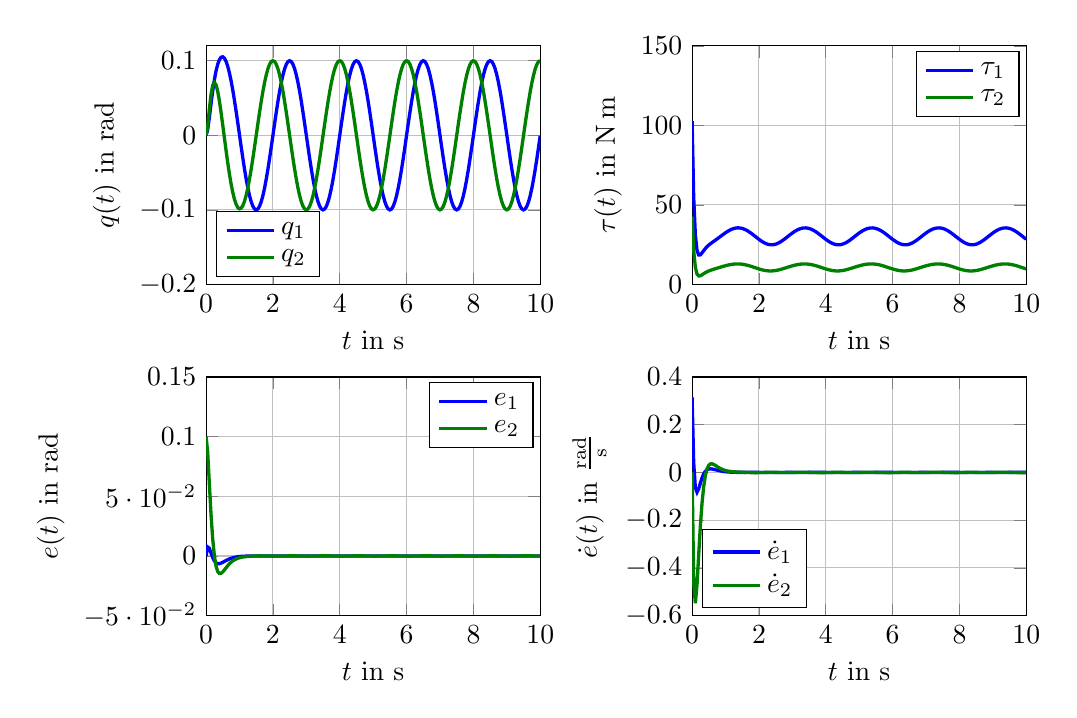
\begin{tikzpicture}

\begin{axis}[%
width=0.35\textwidth,
height=0.25\textwidth,
scale only axis,
xmin=0,
xmax=10,
xlabel={$t$ in $\mathrm{s}$},
xmajorgrids,
ymin=-0.2,
ymax=0.12,
ylabel={$q(t)$ in $\mathrm{rad}$},
ymajorgrids,
name=plot1,
legend style={at={(0.03,0.03)},anchor=south west,draw=black,fill=white,legend cell align=left}
]
\addplot [
color=blue,
solid,
line width=1.2pt
]
table[row sep=crcr]{
0 0\\
0.0474177202323595 0.00731306594338191\\
0.0974177202323595 0.0236547644873976\\
0.14741772023236 0.042079325134868\\
0.19741772023236 0.0593743023768626\\
0.24741772023236 0.0742136739500476\\
0.29741772023236 0.0861595150883708\\
0.34741772023236 0.0951525316162058\\
0.39741772023236 0.101269074044196\\
0.44741772023236 0.10461844733222\\
0.49741772023236 0.105310075322709\\
0.54741772023236 0.103452245376777\\
0.59741772023236 0.0991624758527611\\
0.64741772023236 0.0925797465939553\\
0.69741772023236 0.0838743263173214\\
0.74741772023236 0.073253754976106\\
0.79741772023236 0.0609648917076844\\
0.84741772023236 0.0472925118733525\\
0.89741772023236 0.0325551192302674\\
0.94741772023236 0.0170986428328155\\
0.99741772023236 0.00128862221215651\\
1.04741772023236 -0.0144985985954692\\
1.09741772023235 -0.0298852250972957\\
1.14741772023234 -0.0445015362969548\\
1.19741772023234 -0.0579952526930399\\
1.24741772023233 -0.0700404650231225\\
1.29741772023233 -0.0803458767678189\\
1.34741772023232 -0.0886621466726667\\
1.39741772023232 -0.0947881501021197\\
1.44741772023231 -0.0985760113476088\\
1.49741772023231 -0.099934793569382\\
1.5474177202323 -0.098832768563938\\
1.59741772023229 -0.0952982241919773\\
1.64741772023229 -0.0894188020776383\\
1.69741772023228 -0.08133939127736\\
1.74741772023228 -0.0712586346098538\\
1.79741772023227 -0.0594241332796788\\
1.84741772023227 -0.0461264626265132\\
1.89741772023226 -0.0316921375625108\\
1.94741772023226 -0.0164756904643891\\
1.99741772023225 -0.000851046434995108\\
2.04741772023225 0.0147976000085601\\
2.09741772023224 0.0300851877804455\\
2.14741772023223 0.0446352428203163\\
2.19741772023223 0.0580891499020575\\
2.24741772023222 0.0701150126754377\\
2.29741772023222 0.0804158806635643\\
2.34741772023221 0.0887371363050547\\
2.39741772023221 0.0948728545117759\\
2.4474177202322 0.0986709710061857\\
2.4974177202322 0.100037123479917\\
2.54741772023219 0.0989370611449333\\
2.59741772023218 0.0953975533618003\\
2.64741772023218 0.0895057663781044\\
2.69741772023217 0.0814071180099866\\
2.74741772023217 0.071301661994422\\
2.79741772023216 0.0594390948766801\\
2.84741772023216 0.0461125166172627\\
2.89741772023215 0.0316511097354421\\
2.94741772023215 0.0164119294128683\\
2.99741772023214 0.000771017911654532\\
3.04741772023214 -0.014885929101107\\
3.09741772023213 -0.0301731087943775\\
3.14741772023212 -0.0447141322888619\\
3.19741772023212 -0.0581512861238994\\
3.24741772023211 -0.0701543078006664\\
3.29741772023211 -0.0804284623837212\\
3.3474177202321 -0.0887217253941493\\
3.3974177202321 -0.0948309003460637\\
3.44741772023209 -0.0986065268548041\\
3.49741772023209 -0.0999564664821887\\
3.54741772023208 -0.0988480872045434\\
3.59741772023207 -0.09530900218502\\
3.64741772023207 -0.0894263530242222\\
3.69741772023206 -0.0813446607879958\\
3.74741772023206 -0.0712622993093445\\
3.79741772023205 -0.0594266744811818\\
3.84741772023205 -0.0461282207530268\\
3.89741772023204 -0.0316933520586235\\
3.94741772023204 -0.0164765288603313\\
3.99741772023203 -0.000851625363652437\\
4.04741772023205 0.0147971997187284\\
4.09741772023206 0.0300849103409234\\
4.14741772023208 0.0446350498569802\\
4.1974177202321 0.0580890150890068\\
4.24741772023211 0.0701149179830851\\
4.29741772023213 0.0804158137516168\\
4.34741772023215 0.0887370887216388\\
4.39741772023216 0.0948728204561888\\
4.44741772023218 0.0986709464830217\\
4.4974177202322 0.100037105723184\\
4.54741772023221 0.0989370482272727\\
4.59741772023223 0.0953975439298779\\
4.64741772023225 0.0895057594735733\\
4.69741772023226 0.0814071129482235\\
4.74741772023228 0.0713016582821455\\
4.7974177202323 0.0594390921556841\\
4.84741772023231 0.0461125146256916\\
4.89741772023233 0.031651108280875\\
4.94741772023235 0.0164119283533947\\
4.99741772023236 0.000771017142401895\\
5.04741772023238 -0.0148859296576828\\
5.0974177202324 -0.030173109195571\\
5.14741772023241 -0.0447141325769282\\
5.19741772023243 -0.0581512863299174\\
5.24741772023245 -0.0701543079474174\\
5.29741772023246 -0.0804284624878395\\
5.34741772023248 -0.0887217254677294\\
5.3974177202325 -0.0948309003978601\\
5.44741772023251 -0.0986065268911252\\
5.49741772023253 -0.099956466507559\\
5.54741772023255 -0.0988480872221932\\
5.59741772023256 -0.0953090021972456\\
5.64741772023258 -0.0894263530326487\\
5.6974177202326 -0.0813446607937688\\
5.74741772023261 -0.0712622993132684\\
5.79741772023263 -0.05942667448382\\
5.84741772023265 -0.0461282207547728\\
5.89741772023266 -0.0316933520597517\\
5.94741772023268 -0.0164765288610331\\
5.9974177202327 -0.000851625364061525\\
6.04741772023271 0.0147971997185178\\
6.09741772023273 0.0300849103408435\\
6.14741772023275 0.044635049856982\\
6.19741772023276 0.058089015089055\\
6.24741772023278 0.0701149179831547\\
6.2974177202328 0.0804158137516898\\
6.34741772023281 0.0887370887217024\\
6.39741772023283 0.0948728204562341\\
6.44741772023285 0.0986709464830429\\
6.49741772023286 0.100037105723178\\
6.54741772023288 0.0989370482272366\\
6.5974177202329 0.0953975439298116\\
6.64741772023291 0.0895057594734776\\
6.69741772023293 0.0814071129481004\\
6.74741772023295 0.0713016582819976\\
6.79741772023296 0.0594390921555148\\
6.84741772023298 0.0461125146255051\\
6.897417720233 0.0316511082806757\\
6.94741772023301 0.0164119283531876\\
6.99741772023303 0.000771017142192006\\
7.04741772023305 -0.0148859296578903\\
7.09741772023306 -0.030173109195771\\
7.14741772023308 -0.0447141325771158\\
7.1974177202331 -0.058151286330088\\
7.24741772023311 -0.0701543079475668\\
7.29741772023313 -0.080428462487964\\
7.34741772023315 -0.0887217254678259\\
7.39741772023316 -0.0948309003979264\\
7.44741772023318 -0.0986065268911595\\
7.4974177202332 -0.0999564665075606\\
7.54741772023321 -0.098848087222162\\
7.59741772023323 -0.0953090021971823\\
7.64741772023325 -0.089426353032555\\
7.69741772023326 -0.0813446607936469\\
7.74741772023328 -0.0712622993131214\\
7.7974177202333 -0.0594266744836515\\
7.84741772023331 -0.0461282207545869\\
7.89741772023333 -0.0316933520595529\\
7.94741772023335 -0.0164765288608263\\
7.99741772023336 -0.000851625363851837\\
8.04741772023334 0.0147971997187245\\
8.09741772023331 0.0300849103410392\\
8.14741772023328 0.0446350498571585\\
8.19741772023326 0.0580890150892064\\
8.24741772023323 0.0701149179832771\\
8.2974177202332 0.0804158137517816\\
8.34741772023317 0.0887370887217641\\
8.39741772023315 0.0948728204562678\\
8.44741772023312 0.0986709464830521\\
8.49741772023309 0.100037105723167\\
8.54741772023306 0.0989370482272107\\
8.59741772023303 0.0953975439297761\\
8.64741772023301 0.0895057594734382\\
8.69741772023298 0.0814071129480622\\
8.74741772023295 0.0713016582819656\\
8.79741772023292 0.0594390921554931\\
8.8474177202329 0.046112514625497\\
8.89741772023287 0.0316511082806836\\
8.94741772023284 0.0164119283532128\\
8.99741772023281 0.000771017142234825\\
9.04741772023278 -0.0148859296578308\\
9.09741772023276 -0.030173109195697\\
9.14741772023273 -0.0447141325770302\\
9.1974177202327 -0.058151286329995\\
9.24741772023267 -0.0701543079474712\\
9.29741772023265 -0.0804284624878711\\
9.34741772023262 -0.0887217254677416\\
9.39741772023259 -0.0948309003978565\\
9.44741772023256 -0.0986065268911099\\
9.49741772023254 -0.0999564665075369\\
9.54741772023251 -0.098848087222169\\
9.59741772023248 -0.0953090021972242\\
9.64741772023245 -0.0894263530326349\\
9.69741772023242 -0.0813446607937668\\
9.7474177202324 -0.0712622993132818\\
9.79741772023237 -0.0594266744838515\\
9.84741772023234 -0.0461282207548243\\
9.89741772023231 -0.0316933520598239\\
9.94741772023229 -0.0164765288611256\\
9.99741772023226 -0.000851625364172748\\
};
\addlegendentry{$q_1$};

\addplot [
color=green!50!black,
solid,
line width=1.2pt
]
table[row sep=crcr]{
0 0\\
0.0474177202323595 0.0118327758995183\\
0.0974177202323595 0.0345391640960716\\
0.14741772023236 0.0544985244637411\\
0.19741772023236 0.0668676446400098\\
0.24741772023236 0.0709639624856355\\
0.29741772023236 0.0678420929256869\\
0.34741772023236 0.0591020749527158\\
0.39741772023236 0.04635107238315\\
0.44741772023236 0.0309966529004521\\
0.49741772023236 0.0141976879090139\\
0.54741772023236 -0.0031178567830941\\
0.59741772023236 -0.0202132948278247\\
0.64741772023236 -0.0365024363117824\\
0.69741772023236 -0.0515157774334454\\
0.74741772023236 -0.0648756691133079\\
0.79741772023236 -0.0762797453725375\\
0.84741772023236 -0.085490897706622\\
0.89741772023236 -0.0923319185119324\\
0.94741772023236 -0.0966831328804034\\
0.99741772023236 -0.0984816559479383\\
1.04741772023236 -0.0977212404844242\\
1.09741772023235 -0.094451970194983\\
1.14741772023234 -0.0887792944980385\\
1.19741772023234 -0.0808620913898409\\
1.24741772023233 -0.0709095929916433\\
1.29741772023233 -0.0591771211946224\\
1.34741772023232 -0.0459606654196485\\
1.39741772023232 -0.0315903966618887\\
1.44741772023231 -0.0164232564791825\\
1.49741772023231 -0.000834790579120447\\
1.5474177202323 0.0147895820517401\\
1.59741772023229 0.0300636586185442\\
1.64741772023229 0.0446096836533101\\
1.69741772023228 0.0580674963357257\\
1.74741772023228 0.0701033626907751\\
1.79741772023227 0.0804182597332264\\
1.84741772023227 0.0887553834051081\\
1.89741772023226 0.0949066653267844\\
1.94741772023226 0.0987181059666697\\
1.99741772023225 0.100093763430479\\
2.04741772023225 0.098998275952665\\
2.09741772023224 0.0954578397794777\\
2.14741772023223 0.0895596097335734\\
2.19741772023223 0.0814495350286548\\
2.24741772023222 0.0713286862925867\\
2.29741772023222 0.0594481704630298\\
2.34741772023221 0.0461027679646162\\
2.39741772023221 0.0316234611874638\\
2.4474177202322 0.0163690542580185\\
2.4974177202322 0.0007171103032069\\
2.54741772023219 -0.0149455478675426\\
2.59741772023218 -0.0302325164561984\\
2.64741772023218 -0.04476741023672\\
2.69741772023217 -0.0581931335865666\\
2.74741772023217 -0.0701805920702133\\
2.79741772023216 -0.0804366390800937\\
2.84741772023216 -0.0887110812798025\\
2.89741772023215 -0.094802596708195\\
2.94741772023215 -0.098563448427866\\
2.99741772023214 -0.0999029039053233\\
3.04741772023214 -0.0987892964249381\\
3.09741772023213 -0.0952506909114684\\
3.14741772023212 -0.0893741436627905\\
3.19741772023212 -0.0813035741892857\\
3.24741772023211 -0.071236297303679\\
3.29741772023211 -0.0594182937266374\\
3.3474177202321 -0.0461383262459574\\
3.3974177202321 -0.0317210343795783\\
3.44741772023209 -0.0165191625025422\\
3.49741772023209 -0.000905094240834671\\
3.54741772023208 0.0147381198431835\\
3.59741772023207 0.030026042594805\\
3.64741772023207 0.0445822298865429\\
3.69741772023206 0.0580474919739962\\
3.74741772023206 0.0700888123696388\\
3.79741772023205 0.0804076973192665\\
3.84741772023205 0.0887477326530021\\
3.89741772023204 0.0949011369630377\\
3.94741772023204 0.0987141217900217\\
3.99741772023203 0.100090900389751\\
4.04741772023205 0.0989962249667029\\
4.09741772023206 0.0954563754224121\\
4.14741772023208 0.0895585679234806\\
4.1974177202321 0.0814487966108773\\
4.24741772023211 0.0713281649653707\\
4.29741772023213 0.0594478039028329\\
4.34741772023215 0.0461025113096171\\
4.39741772023216 0.0316232822591034\\
4.44741772023218 0.016368930063099\\
4.4974177202322 0.000717024478832626\\
4.54741772023221 -0.0149456069156087\\
4.59741772023223 -0.0302325569059926\\
4.64741772023225 -0.0447674378293714\\
4.69741772023226 -0.0581931523327709\\
4.74741772023228 -0.0701806047578136\\
4.7974177202323 -0.0804366476371376\\
4.84741772023231 -0.0887110870329755\\
4.89741772023233 -0.0948026005658346\\
4.94741772023235 -0.0985634510088607\\
4.99741772023236 -0.099902905629386\\
5.04741772023238 -0.0987892975754594\\
5.0974177202324 -0.0952506916790232\\
5.14741772023241 -0.0893741441750739\\
5.19741772023243 -0.0813035745315941\\
5.24741772023245 -0.0712362975328434\\
5.29741772023246 -0.0594182938804517\\
5.34741772023248 -0.0461383263495262\\
5.3974177202325 -0.0317210344495713\\
5.44741772023251 -0.0165191625500341\\
5.49741772023253 -0.000905094273192895\\
5.54741772023255 0.014738119821046\\
5.59741772023256 0.0300260425796013\\
5.64741772023258 0.0445822298760652\\
5.6974177202326 0.0580474919667539\\
5.74741772023261 0.0700888123646198\\
5.79741772023263 0.0804076973157797\\
5.84741772023265 0.0887477326505722\\
5.89741772023266 0.0949011369613362\\
5.94741772023268 0.0987141217888201\\
5.9974177202327 0.10009090038889\\
6.04741772023271 0.0989962249660696\\
6.09741772023273 0.0954563754219294\\
6.14741772023275 0.0895585679230951\\
6.19741772023276 0.0814487966105528\\
6.24741772023278 0.0713281649650833\\
6.2974177202328 0.0594478039025674\\
6.34741772023281 0.0461025113093644\\
6.39741772023283 0.0316232822588588\\
6.44741772023285 0.016368930062861\\
6.49741772023286 0.00071702447860183\\
6.54741772023288 -0.0149456069158303\\
6.5974177202329 -0.030232556906202\\
6.64741772023291 -0.0447674378295652\\
6.69741772023293 -0.0581931523329455\\
6.74741772023295 -0.0701806047579655\\
6.79741772023296 -0.0804366476372636\\
6.84741772023298 -0.0887110870330729\\
6.897417720233 -0.0948026005659014\\
6.94741772023301 -0.0985634510088954\\
6.99741772023303 -0.0999029056293878\\
7.04741772023305 -0.0987892975754285\\
7.09741772023306 -0.0952506916789602\\
7.14741772023308 -0.0893741441749804\\
7.1974177202331 -0.0813035745314725\\
7.24741772023311 -0.0712362975326967\\
7.29741772023313 -0.0594182938802834\\
7.34741772023315 -0.0461383263493405\\
7.39741772023316 -0.0317210344493727\\
7.44741772023318 -0.0165191625498274\\
7.4974177202332 -0.00090509427298332\\
7.54741772023321 0.0147381198212534\\
7.59741772023323 0.0300260425798015\\
7.64741772023325 0.0445822298762532\\
7.69741772023326 0.058047491966925\\
7.74741772023328 0.0700888123647697\\
7.7974177202333 0.0804076973159048\\
7.84741772023331 0.0887477326506695\\
7.89741772023333 0.0949011369614031\\
7.94741772023335 0.098714121788855\\
7.99741772023336 0.100090900388892\\
8.04741772023334 0.0989962249660388\\
8.09741772023331 0.0954563754218687\\
8.14741772023328 0.0895585679230092\\
8.19741772023326 0.0814487966104476\\
8.24741772023323 0.0713281649649653\\
8.2974177202332 0.0594478039024432\\
8.34741772023317 0.0461025113092403\\
8.39741772023315 0.0316232822587406\\
8.44741772023312 0.0163689300627535\\
8.49741772023309 0.000717024478508947\\
8.54741772023306 -0.0149456069159058\\
8.59741772023303 -0.0302325569062587\\
8.64741772023301 -0.0447674378296026\\
8.69741772023298 -0.0581931523329646\\
8.74741772023295 -0.0701806047579682\\
8.79741772023292 -0.0804366476372528\\
8.8474177202329 -0.0887110870330523\\
8.89741772023287 -0.0948026005658752\\
8.94741772023284 -0.0985634510088684\\
8.99741772023281 -0.0999029056293649\\
9.04741772023278 -0.0987892975754146\\
9.09741772023276 -0.09525069167896\\
9.14741772023273 -0.089374144174998\\
9.1974177202327 -0.0813035745315113\\
9.24741772023267 -0.0712362975327592\\
9.29741772023265 -0.0594182938803713\\
9.34741772023262 -0.0461383263494541\\
9.39741772023259 -0.0317210344495113\\
9.44741772023256 -0.016519162549989\\
9.49741772023254 -0.000905094273164656\\
9.54741772023251 0.0147381198210567\\
9.59741772023248 0.0300260425795949\\
9.64741772023245 0.044582229876043\\
9.69741772023242 0.0580474919667185\\
9.7474177202324 0.0700888123645745\\
9.79741772023237 0.0804076973157286\\
9.84741772023234 0.0887477326505204\\
9.89741772023231 0.0949011369612886\\
9.94741772023229 0.0987141217887821\\
9.99741772023226 0.100090900388867\\
};
\addlegendentry{$q_2$};

\end{axis}

\begin{axis}[%
width=0.35\textwidth,
height=0.25\textwidth,
scale only axis,
xmin=0,
xmax=10,
xlabel={$t$ in $\mathrm{s}$},
xmajorgrids,
ymin=-0.05,
ymax=0.15,
ylabel={$e(t)$ in $\mathrm{rad}$},
ymajorgrids,
name=plot3,
at=(plot1.below south west),
anchor=above north west,
legend style={draw=black,fill=white,legend cell align=left}
]
\addplot [
color=blue,
solid,
line width=1.2pt
]
table[row sep=crcr]{
0 0\\
0.0474177202323595 0.00752861527090153\\
0.0974177202323595 0.00647438470941568\\
0.14741772023236 0.00259541239833619\\
0.19741772023236 -0.00125401681228837\\
0.24741772023236 -0.00407895467487211\\
0.29741772023236 -0.00573731165493717\\
0.34741772023236 -0.00642310557903603\\
0.39741772023236 -0.00641723834840692\\
0.44741772023236 -0.00597976896783679\\
0.49741772023236 -0.00531336591406795\\
0.54741772023236 -0.00455975577957063\\
0.59741772023236 -0.00380926736622841\\
0.64741772023236 -0.00311373167019052\\
0.69741772023236 -0.00249845516442783\\
0.74741772023236 -0.00197177161290042\\
0.79741772023236 -0.00153199513590856\\
0.84741772023236 -0.00117213725307862\\
0.89741772023236 -0.00088290324939435\\
0.94741772023236 -0.000654460562850893\\
0.99741772023236 -0.00047738399569879\\
1.04741772023236 -0.000343082618812825\\
1.09741772023235 -0.000243924099514521\\
1.14741772023234 -0.000173201236245042\\
1.19741772023234 -0.000125032871528971\\
1.24741772023233 -9.42542520471074e-05\\
1.29741772023233 -7.63266656086947e-05\\
1.34741772023232 -6.72793644976161e-05\\
1.39741772023232 -6.36855936648612e-05\\
1.44741772023231 -6.26670167715448e-05\\
1.49741772023231 -6.19158392586444e-05\\
1.5474177202323 -5.97210332712039e-05\\
1.59741772023229 -5.49842945615636e-05\\
1.64741772023229 -4.7212846136499e-05\\
1.69741772023228 -3.64798755475709e-05\\
1.74741772023228 -2.33487533698173e-05\\
1.79741772023227 -8.76329211912941e-06\\
1.84741772023227 6.08800621330202e-06\\
1.89741772023226 1.99215816083925e-05\\
1.94741772023226 3.15081943920818e-05\\
1.99741772023225 3.98082185029197e-05\\
2.04741772023225 4.40812056877876e-05\\
2.09741772023224 4.39614163317732e-05\\
2.14741772023223 3.94947128525627e-05\\
2.19741772023223 3.11356624832435e-05\\
2.24741772023222 1.97065997072782e-05\\
2.29741772023222 6.32276984280367e-06\\
2.34741772023221 -7.71026790624685e-06\\
2.39741772023221 -2.10188160022634e-05\\
2.4474177202322 -3.22926418110381e-05\\
2.4974177202322 -4.04140712762929e-05\\
2.54741772023219 -4.4571547718919e-05\\
2.59741772023218 -4.43448752510123e-05\\
2.64741772023218 -3.97514543141325e-05\\
2.69741772023217 -3.12468570589364e-05\\
2.74741772023217 -1.96786311741637e-05\\
2.79741772023216 -6.19830485425882e-06\\
2.84741772023216 7.85800306783713e-06\\
2.89741772023215 2.11062454931188e-05\\
2.94741772023215 3.22528571626429e-05\\
2.99741772023214 4.02203048723061e-05\\
3.04741772023214 4.42478868933407e-05\\
3.09741772023213 4.39595976331614e-05\\
3.14741772023212 3.9394755723926e-05\\
3.19741772023212 3.10005593869497e-05\\
3.24741772023211 1.95885255461353e-05\\
3.29741772023211 6.25895033468105e-06\\
3.3474177202321 -7.70064298315221e-06\\
3.3974177202321 -2.09353496990056e-05\\
3.44741772023209 -3.21515095649122e-05\\
3.49741772023209 -4.02429264514392e-05\\
3.54741772023208 -4.44023926761267e-05\\
3.59741772023207 -4.42063015396593e-05\\
3.64741772023207 -3.96618995835013e-05\\
3.69741772023206 -3.12103649519196e-05\\
3.74741772023206 -1.96840539276599e-05\\
3.79741772023205 -6.22209067178275e-06\\
3.84741772023205 7.84613266551631e-06\\
3.89741772023204 2.11360776554842e-05\\
3.94741772023204 3.23465902661649e-05\\
3.99741772023203 4.03871470911261e-05\\
4.04741772023205 4.44814954574917e-05\\
4.09741772023206 4.42388558007101e-05\\
4.14741772023208 3.96876761450254e-05\\
4.1974177202321 3.12704754998894e-05\\
4.24741772023211 1.98012920349655e-05\\
4.29741772023213 6.38968177371635e-06\\
4.34741772023215 -7.66268449997609e-06\\
4.39741772023216 -2.09847604195068e-05\\
4.44741772023218 -3.22681186481488e-05\\
4.4974177202322 -4.03963145438474e-05\\
4.54741772023221 -4.45586300594492e-05\\
4.59741772023223 -4.43354433328769e-05\\
4.64741772023225 -3.97445497924559e-05\\
4.69741772023226 -3.12417953122202e-05\\
4.74741772023228 -1.96749189221995e-05\\
4.7974177202323 -6.19558389210184e-06\\
4.84741772023231 7.85999459543968e-06\\
4.89741772023233 2.11077000071419e-05\\
4.94741772023235 3.22539165742847e-05\\
4.99741772023236 4.02210740549823e-05\\
5.04741772023238 4.42484433930863e-05\\
5.0974177202324 4.39599987468869e-05\\
5.14741772023241 3.9395043709034e-05\\
5.19741772023243 3.10007653251815e-05\\
5.24741772023245 1.95886722225286e-05\\
5.29741772023246 6.25905438643437e-06\\
5.34741772023248 -7.70056945779973e-06\\
5.3974177202325 -2.09352979423927e-05\\
5.44741772023251 -3.21514732656153e-05\\
5.49741772023253 -4.0242901082288e-05\\
5.54741772023255 -4.44023750045403e-05\\
5.59741772023256 -4.42062892678091e-05\\
5.64741772023258 -3.96618910853269e-05\\
5.6974177202326 -3.1210359081546e-05\\
5.74741772023261 -1.96840498814105e-05\\
5.79741772023263 -6.22208788755851e-06\\
5.84741772023265 7.84613457877059e-06\\
5.89741772023266 2.11360789691695e-05\\
5.94741772023268 3.23465911674856e-05\\
5.9974177202327 4.03871477096156e-05\\
6.04741772023271 4.44814958755254e-05\\
6.09741772023273 4.42388560808159e-05\\
6.14741772023275 3.96876763309323e-05\\
6.19741772023276 3.12704756224788e-05\\
6.24741772023278 1.98012921149432e-05\\
6.2974177202328 6.38968182552213e-06\\
6.34741772023281 -7.66268446689145e-06\\
6.39741772023283 -2.09847603984403e-05\\
6.44741772023285 -3.22681186348955e-05\\
6.49741772023286 -4.0396314535604e-05\\
6.54741772023288 -4.45586300543699e-05\\
6.5974177202329 -4.43354433297821e-05\\
6.64741772023291 -3.97445497904159e-05\\
6.69741772023293 -3.12417953109573e-05\\
6.74741772023295 -1.96749189215611e-05\\
6.79741772023296 -6.19558389156755e-06\\
6.84741772023298 7.85999459568948e-06\\
6.897417720233 2.11077000074264e-05\\
6.94741772023301 3.22539165743194e-05\\
6.99741772023303 4.02210740551145e-05\\
7.04741772023305 4.42484433929736e-05\\
7.09741772023306 4.39599987466996e-05\\
7.14741772023308 3.9395043708805e-05\\
7.1974177202331 3.10007653252092e-05\\
7.24741772023311 1.95886722221955e-05\\
7.29741772023313 6.25905438643437e-06\\
7.34741772023315 -7.70056945806341e-06\\
7.39741772023316 -2.09352979424898e-05\\
7.44741772023318 -3.21514732658373e-05\\
7.4974177202332 -4.02429010823574e-05\\
7.54741772023321 -4.44023750045958e-05\\
7.59741772023323 -4.42062892678785e-05\\
7.64741772023325 -3.96618910852298e-05\\
7.69741772023326 -3.12103590815876e-05\\
7.74741772023328 -1.96840498811329e-05\\
7.7974177202333 -6.22208788751688e-06\\
7.84741772023331 7.84613457908284e-06\\
7.89741772023333 2.11360789691209e-05\\
7.94741772023335 3.23465911677631e-05\\
7.99741772023336 4.0387147709506e-05\\
8.04741772023334 4.44814958630718e-05\\
8.09741772023331 4.42388560589341e-05\\
8.14741772023328 3.9687676305307e-05\\
8.19741772023326 3.12704755968465e-05\\
8.24741772023323 1.9801292092822e-05\\
8.2974177202332 6.38968180888266e-06\\
8.34741772023317 -7.66268447646712e-06\\
8.39741772023315 -2.09847604008551e-05\\
8.44741772023312 -3.22681186301077e-05\\
8.49741772023309 -4.03963145240993e-05\\
8.54741772023306 -4.45586300369533e-05\\
8.59741772023303 -4.43354433072862e-05\\
8.64741772023301 -3.97445497639926e-05\\
8.69741772023298 -3.1241795281467e-05\\
8.74741772023295 -1.96749188902945e-05\\
8.79741772023292 -6.1955838595168e-06\\
8.8474177202329 7.8599946277888e-06\\
8.89741772023287 2.11077000382975e-05\\
8.94741772023284 3.22539166030429e-05\\
8.99741772023281 4.02210740808848e-05\\
9.04741772023278 4.42484434154226e-05\\
9.09741772023276 4.39599987648621e-05\\
9.14741772023273 3.93950437221485e-05\\
9.1974177202327 3.10007653334457e-05\\
9.24741772023267 1.95886722253735e-05\\
9.29741772023265 6.25905438413066e-06\\
9.34741772023262 -7.70056946571007e-06\\
9.39741772023259 -2.09352979553545e-05\\
9.44741772023256 -3.21514732834205e-05\\
9.49741772023254 -4.02429011043953e-05\\
9.54741772023251 -4.44023750305333e-05\\
9.59741772023248 -4.42062892970913e-05\\
9.64741772023245 -3.96618911170238e-05\\
9.69741772023242 -3.1210359115158e-05\\
9.7474177202324 -1.96840499156609e-05\\
9.79741772023237 -6.22208792207951e-06\\
9.84741772023234 7.84613454507532e-06\\
9.89741772023231 2.11360789368273e-05\\
9.94741772023229 3.23465911379571e-05\\
9.99741772023226 4.03871476829486e-05\\
};
\addlegendentry{$e_1$};

\addplot [
color=green!50!black,
solid,
line width=1.2pt
]
table[row sep=crcr]{
0 0.1\\
0.0474177202323595 0.0870597136976882\\
0.0974177202323595 0.0608140443904611\\
0.14741772023236 0.0349674904600238\\
0.19741772023236 0.0145082265128838\\
0.24741772023236 0.000318020877570172\\
0.29741772023236 -0.00840919635391099\\
0.34741772023236 -0.0129817003324418\\
0.39741772023236 -0.0146788564022768\\
0.44741772023236 -0.0145524706304873\\
0.49741772023236 -0.013386449692556\\
0.54741772023236 -0.0117238244311894\\
0.59741772023236 -0.0099158543689887\\
0.64741772023236 -0.00817230122142182\\
0.69741772023236 -0.00660450813112885\\
0.74741772023236 -0.00525905016186769\\
0.79741772023236 -0.00414245806089619\\
0.84741772023236 -0.00323852833054783\\
0.89741772023236 -0.0025199171838565\\
0.94741772023236 -0.00195554548397953\\
0.99741772023236 -0.00151505346070255\\
1.04741772023236 -0.00117124911278249\\
1.09741772023235 -0.000901238291550657\\
1.14741772023234 -0.000686720425728565\\
1.19741772023234 -0.000513779763056582\\
1.24741772023233 -0.000372390371568221\\
1.29741772023233 -0.000255775377161711\\
1.34741772023232 -0.000159709200636002\\
1.39741772023232 -8.18193189973185e-05\\
1.44741772023231 -2.09257907973805e-05\\
1.49741772023231 2.35523626454947e-05\\
1.5474177202323 5.20991625248962e-05\\
1.59741772023229 6.54905782495573e-05\\
1.64741772023229 6.50538798742176e-05\\
1.69741772023228 5.27892288290643e-05\\
1.74741772023228 3.13565843821223e-05\\
1.79741772023227 3.94370019093926e-06\\
1.84741772023227 -2.59573679517594e-05\\
1.89741772023226 -5.4829631005282e-05\\
1.94741772023226 -7.94276022921675e-05\\
1.99741772023225 -9.70540218381277e-05\\
2.04741772023225 -0.000105786355453191\\
2.09741772023224 -0.000104631292933657\\
2.14741772023223 -9.35948097909312e-05\\
2.19741772023223 -7.36638757372482e-05\\
2.24741772023222 -4.67029293510085e-05\\
2.29741772023222 -1.52738912179984e-05\\
2.34741772023221 1.76066556989846e-05\\
2.39741772023221 4.87547934549318e-05\\
2.4474177202322 7.51280119954435e-05\\
2.4974177202322 9.4127913302525e-05\\
2.54741772023219 0.00010386665331171\\
2.59741772023218 0.000103367259437659\\
2.64741772023218 9.26727035666236e-05\\
2.69741772023217 7.28480220399189e-05\\
2.74741772023217 4.58727950806148e-05\\
2.79741772023216 1.4435646696967e-05\\
2.84741772023216 -1.8344757337932e-05\\
2.89741772023215 -4.92389875730997e-05\\
2.94741772023215 -7.52299365058551e-05\\
2.99741772023214 -9.3805503316946e-05\\
3.04741772023214 -0.000103193172278859\\
3.09741772023213 -0.000102517575086072\\
3.14741772023212 -9.18712610073896e-05\\
3.19741772023212 -7.22969636520049e-05\\
3.24741772023211 -4.5686059580996e-05\\
3.29741772023211 -1.46028452022717e-05\\
3.3474177202321 1.79516256115578e-05\\
3.3974177202321 4.8818398626721e-05\\
3.44741772023209 7.49802324940645e-05\\
3.49741772023209 9.38560242905965e-05\\
3.54741772023208 0.000103561371013087\\
3.59741772023207 0.000103106601922909\\
3.64741772023207 9.25076465794761e-05\\
3.69741772023206 7.27935905022042e-05\\
3.74741772023206 4.59069054691563e-05\\
3.79741772023205 1.45061141097885e-05\\
3.84741772023205 -1.83066158776918e-05\\
3.89741772023204 -4.93012672805049e-05\\
3.94741772023204 -7.54434256555886e-05\\
3.99741772023203 -9.41909811114361e-05\\
4.04741772023205 -0.000103735369481814\\
4.09741772023206 -0.000103166935851245\\
4.14741772023208 -9.25529996762958e-05\\
4.1974177202321 -7.29254579353855e-05\\
4.24741772023211 -4.61816021104927e-05\\
4.29741772023213 -1.49073309986675e-05\\
4.34741772023215 1.78633107164317e-05\\
4.39741772023216 4.89337218284314e-05\\
4.44741772023218 7.52522069216374e-05\\
4.4974177202322 9.42137376766459e-05\\
4.54741772023221 0.000103925701370855\\
4.59741772023223 0.00010340770921834\\
4.64741772023225 9.27002961991219e-05\\
4.69741772023226 7.28667682214149e-05\\
4.74741772023228 4.58854826560218e-05\\
4.7974177202323 1.44442037158243e-05\\
4.84741772023231 -1.83390041875731e-05\\
4.89741772023233 -4.92351299512805e-05\\
4.94741772023235 -7.52273555214983e-05\\
4.99741772023236 -9.38037792548724e-05\\
5.04741772023238 -0.000103192021746065\\
5.0974177202324 -0.000102516807506101\\
5.14741772023241 -9.18707486834841e-05\\
5.19741772023243 -7.22966212866188e-05\\
5.24741772023245 -4.56858303431035e-05\\
5.29741772023246 -1.46026912979588e-05\\
5.34741772023248 1.79517292856132e-05\\
5.3974177202325 4.88184687390605e-05\\
5.44741772023251 7.49802801167793e-05\\
5.49741772023253 9.38560567885906e-05\\
5.54741772023255 0.00010356139329552\\
5.59741772023256 0.00010310661727303\\
5.64741772023258 9.25076572007785e-05\\
5.6974177202326 7.27935978809754e-05\\
5.74741772023261 4.59069106125004e-05\\
5.79741772023263 1.45061177045103e-05\\
5.84741772023265 -1.83066133608717e-05\\
5.89741772023266 -4.93012655171238e-05\\
5.94741772023268 -7.54434244207153e-05\\
5.9974177202327 -9.41909802482516e-05\\
6.04741772023271 -0.000103735368879657\\
6.09741772023273 -0.000103166935431845\\
6.14741772023275 -9.25529993845153e-05\\
6.19741772023276 -7.29254577329364e-05\\
6.24741772023278 -4.61816019702577e-05\\
6.2974177202328 -1.49073309020017e-05\\
6.34741772023281 1.78633107831908e-05\\
6.39741772023283 4.89337218740338e-05\\
6.44741772023285 7.52522069528937e-05\\
6.49741772023286 9.42137376976849e-05\\
6.54741772023288 0.000103925701385156\\
6.5974177202329 0.000103407709227704\\
6.64741772023291 9.27002962054016e-05\\
6.69741772023293 7.28667682253423e-05\\
6.74741772023295 4.58854826583116e-05\\
6.79741772023296 1.44442037171705e-05\\
6.84741772023298 -1.83390041869208e-05\\
6.897417720233 -4.92351299509336e-05\\
6.94741772023301 -7.52273555213318e-05\\
6.99741772023303 -9.38037792547614e-05\\
7.04741772023305 -0.000103192021745885\\
7.09741772023306 -0.000102516807505823\\
7.14741772023308 -9.18707486831649e-05\\
7.1974177202331 -7.22966212864662e-05\\
7.24741772023311 -4.568583034259e-05\\
7.29741772023313 -1.46026912977021e-05\\
7.34741772023315 1.79517292861822e-05\\
7.39741772023316 4.88184687392618e-05\\
7.44741772023318 7.49802801172407e-05\\
7.4974177202332 9.38560567885945e-05\\
7.54741772023321 0.000103561393295745\\
7.59741772023323 0.000103106617272756\\
7.64741772023325 9.25076572006744e-05\\
7.69741772023326 7.27935978804689e-05\\
7.74741772023328 4.59069106121812e-05\\
7.7974177202333 1.45061177039274e-05\\
7.84741772023331 -1.83066133613019e-05\\
7.89741772023333 -4.93012655176234e-05\\
7.94741772023335 -7.54434244210345e-05\\
7.99741772023336 -9.41909802484042e-05\\
8.04741772023334 -0.000103735368878005\\
8.09741772023331 -0.000103166935426044\\
8.14741772023328 -9.25529993739682e-05\\
8.19741772023326 -7.2925457717532e-05\\
8.24741772023323 -4.61816019508982e-05\\
8.2974177202332 -1.49073308795128e-05\\
8.34741772023317 1.78633108070189e-05\\
8.39741772023315 4.89337218985905e-05\\
8.44741772023312 7.5252206976642e-05\\
8.49741772023309 9.42137377198957e-05\\
8.54741772023306 0.000103925701404165\\
8.59741772023303 0.000103407709243431\\
8.64741772023301 9.27002962168091e-05\\
8.69741772023298 7.28667682323089e-05\\
8.74741772023295 4.58854826602129e-05\\
8.79741772023292 1.44442037139508e-05\\
8.8474177202329 -1.83390041950948e-05\\
8.89741772023287 -4.9235129964173e-05\\
8.94741772023284 -7.52273555393174e-05\\
8.99741772023281 -9.38037792770491e-05\\
9.04741772023278 -0.000103192021771989\\
9.09741772023276 -0.000102516807535175\\
9.14741772023273 -9.18707487149867e-05\\
9.1974177202327 -7.22966213199394e-05\\
9.24741772023267 -4.56858303772567e-05\\
9.29741772023265 -1.46026913324382e-05\\
9.34741772023262 1.7951729252251e-05\\
9.39741772023259 4.88184687069959e-05\\
9.44741772023256 7.4980280087119e-05\\
9.49741772023254 9.38560567617236e-05\\
9.54741772023251 0.000103561393272824\\
9.59741772023248 0.000103106617254382\\
9.64741772023245 9.25076571870187e-05\\
9.69741772023242 7.27935978721561e-05\\
9.7474177202324 4.59069106093918e-05\\
9.79741772023237 1.45061177067446e-05\\
9.84741772023234 -1.83066133532944e-05\\
9.89741772023231 -4.9301265504384e-05\\
9.94741772023229 -7.54434244030072e-05\\
9.99741772023226 -9.41909802261581e-05\\
};
\addlegendentry{$e_2$};

\end{axis}

\begin{axis}[%
width=0.35\textwidth,
height=0.25\textwidth,
scale only axis,
xmin=0,
xmax=10,
xlabel={$t$ in $\mathrm{s}$},
xmajorgrids,
ymin=-0.6,
ymax=0.4,
ylabel={$\dot{e}(t)$ in $\mathrm{\frac{rad}{s}}$},
ymajorgrids,
name=plot2,
at=(plot3.right of south east),
anchor=left of south west,
legend style={at={(0.03,0.03)},anchor=south west,draw=black,fill=white,legend cell align=left}
]
\addplot [
color=blue,
solid,
line width=1.2pt
]
table[row sep=crcr]{
0 0.314159265358979\\
0.0474177202323595 0.0421268714137853\\
0.0974177202323595 -0.063516797254402\\
0.14741772023236 -0.0829274912800539\\
0.19741772023236 -0.0683287119796598\\
0.24741772023236 -0.044703673933091\\
0.29741772023236 -0.0227611779769814\\
0.34741772023236 -0.00609628052209016\\
0.39741772023236 0.00495810370055133\\
0.44741772023236 0.011342570258207\\
0.49741772023236 0.0143086483246096\\
0.54741772023236 0.0150024049265735\\
0.59741772023236 0.0143242405109794\\
0.64741772023236 0.0129173211093033\\
0.69741772023236 0.0112073136271114\\
0.74741772023236 0.00945535476145698\\
0.79741772023236 0.00780737921375013\\
0.84741772023236 0.00633382064882354\\
0.89741772023236 0.0050588838281061\\
0.94741772023236 0.00398074232176815\\
0.99741772023236 0.00308465332898339\\
1.04741772023236 0.00235092292827727\\
1.09741772023235 0.00175933073655821\\
1.14741772023234 0.00129124250530255\\
1.19741772023234 0.000930295432647443\\
1.24741772023233 0.000662266737958106\\
1.29741772023233 0.00047453493357405\\
1.34741772023232 0.000355405393855729\\
1.39741772023232 0.000293481782214736\\
1.44741772023231 0.000277205632819098\\
1.49741772023231 0.000294642150392125\\
1.5474177202323 0.000333549175425739\\
1.59741772023229 0.000381722374906579\\
1.64741772023229 0.000427564169018069\\
1.69741772023228 0.000460783647190793\\
1.74741772023228 0.000473109178619979\\
1.79741772023227 0.000458891953971419\\
1.84741772023227 0.000415498944624282\\
1.89741772023226 0.000343432480306438\\
1.94741772023226 0.000246160511614302\\
1.99741772023225 0.000129685061471263\\
2.04741772023225 1.90745286815508e-06\\
2.09741772023224 -0.000128136210749585\\
2.14741772023223 -0.000251095613799157\\
2.19741772023223 -0.00035811824133003\\
2.24741772023222 -0.000441599966475997\\
2.29741772023222 -0.00049583024245109\\
2.34741772023221 -0.000517491599488135\\
2.39741772023221 -0.000505973069912652\\
2.4474177202322 -0.000463458152057977\\
2.4974177202322 -0.000394756203536939\\
2.54741772023219 -0.000306866478005159\\
2.59741772023218 -0.000208296785092127\\
2.64741772023218 -0.000108198529190501\\
2.69741772023217 -1.54164469643447e-05\\
2.74741772023217 6.24267394265243e-05\\
2.79741772023216 0.000119691346280482\\
2.84741772023216 0.000153232667632786\\
2.89741772023215 0.000162611184884587\\
2.94741772023215 0.000149996693810495\\
2.99741772023214 0.000119804556353464\\
3.04741772023214 7.81306222865652e-05\\
3.09741772023213 3.20625612670322e-05\\
3.14741772023212 -1.10581026067091e-05\\
3.19741772023212 -4.43610282100382e-05\\
3.24741772023211 -6.21106858309517e-05\\
3.29741772023211 -6.02700882513796e-05\\
3.3474177202321 -3.69301179136694e-05\\
3.3974177202321 7.43056786393914e-06\\
3.44741772023209 6.98903750088534e-05\\
3.49741772023209 0.000145263665074497\\
3.54741772023208 0.00022652581445546\\
3.59741772023207 0.000305467196490022\\
3.64741772023207 0.000373521771387442\\
3.69741772023206 0.000422680354143029\\
3.74741772023206 0.00044637534088704\\
3.79741772023205 0.000440221023447096\\
3.84741772023205 0.000402513855814968\\
3.89741772023204 0.000334435288723955\\
3.94741772023204 0.000239945988279422\\
3.99741772023203 0.000125402968953692\\
4.04741772023205 -1.03844237536732e-06\\
4.09741772023206 -0.000130161633687731\\
4.14741772023208 -0.000252488869098344\\
4.1974177202321 -0.000359078276186975\\
4.24741772023211 -0.000442263459507986\\
4.29741772023213 -0.000496290742295152\\
4.34741772023215 -0.00051781294994252\\
4.39741772023216 -0.000506198761878365\\
4.44741772023218 -0.000463617794516098\\
4.4974177202322 -0.000394869972560308\\
4.54741772023221 -0.00030694815738088\\
4.59741772023223 -0.000208355833088023\\
4.64741772023225 -0.000108241476685783\\
4.69741772023226 -1.54478396201807e-05\\
4.74741772023228 6.24037079324791e-05\\
4.7974177202323 0.000119674409076731\\
4.84741772023231 0.000153220198846005\\
4.89741772023233 0.000162602006794133\\
4.94741772023235 0.000149989945843865\\
4.99741772023236 0.000119799605211635\\
5.04741772023238 7.81269995021039e-05\\
5.0974177202324 3.20599191855897e-05\\
5.14741772023241 -1.10600223362511e-05\\
5.19741772023243 -4.43624175252566e-05\\
5.24741772023245 -6.21116870964389e-05\\
5.29741772023246 -6.02708067789226e-05\\
5.34741772023248 -3.69306313321438e-05\\
5.3974177202325 7.43020256813165e-06\\
5.44741772023251 6.98901161891516e-05\\
5.49741772023253 0.000145263482441063\\
5.54741772023255 0.000226525686084125\\
5.59741772023256 0.000305467106593266\\
5.64741772023258 0.000373521708649432\\
5.6974177202326 0.000422680310494861\\
5.74741772023261 0.0004463753106006\\
5.79741772023263 0.000440221002477259\\
5.84741772023265 0.000402513841315788\\
5.89741772023266 0.000334435278704415\\
5.94741772023268 0.000239945981350742\\
5.9974177202327 0.000125402964152865\\
6.04741772023271 -1.03844569226963e-06\\
6.09741772023273 -0.000130161635956971\\
6.14741772023275 -0.000252488870636391\\
6.19741772023276 -0.000359078277220815\\
6.24741772023278 -0.000442263460196851\\
6.2974177202328 -0.000496290742750677\\
6.34741772023281 -0.000517812950240421\\
6.39741772023283 -0.000506198762072183\\
6.44741772023285 -0.000463617794639812\\
6.49741772023286 -0.000394869972639197\\
6.54741772023288 -0.00030694815742939\\
6.5974177202329 -0.000208355833117721\\
6.64741772023291 -0.000108241476703214\\
6.69741772023293 -1.54478396309776e-05\\
6.74741772023295 6.24037079268447e-05\\
6.79741772023296 0.000119674409073567\\
6.84741772023298 0.00015322019884384\\
6.897417720233 0.000162602006792911\\
6.94741772023301 0.000149989945842866\\
6.99741772023303 0.000119799605210802\\
7.04741772023305 7.81269995012157e-05\\
7.09741772023306 3.20599191849791e-05\\
7.14741772023308 -1.10600223366397e-05\\
7.1974177202331 -4.43624175253676e-05\\
7.24741772023311 -6.21116870961891e-05\\
7.29741772023313 -6.02708067793112e-05\\
7.34741772023315 -3.69306313313944e-05\\
7.39741772023316 7.43020256833982e-06\\
7.44741772023318 6.98901161908724e-05\\
7.4974177202332 0.000145263482441853\\
7.54741772023321 0.000226525686086103\\
7.59741772023323 0.000305467106594084\\
7.64741772023325 0.000373521708651264\\
7.69741772023326 0.000422680310495305\\
7.74741772023328 0.000446375310601432\\
7.7974177202333 0.000440221002476537\\
7.84741772023331 0.000402513841315288\\
7.89741772023333 0.000334435278703193\\
7.94741772023335 0.000239945981349632\\
7.99741772023336 0.0001254029641512\\
8.04741772023334 -1.03844564813826e-06\\
8.09741772023331 -0.000130161635824688\\
8.14741772023328 -0.000252488870423506\\
8.19741772023326 -0.000359078276953695\\
8.24741772023323 -0.00044226345990428\\
8.2974177202332 -0.000496290742457745\\
8.34741772023317 -0.000517812949969221\\
8.39741772023315 -0.000506198761838966\\
8.44741772023312 -0.000463617794455834\\
8.49741772023309 -0.000394869972510723\\
8.54741772023306 -0.000306948157361903\\
8.59741772023303 -0.000208355833112836\\
8.64741772023301 -0.000108241476759835\\
8.69741772023298 -1.54478397454139e-05\\
8.74741772023295 6.24037077575634e-05\\
8.79741772023292 0.000119674408854686\\
8.8474177202329 0.000153220198582438\\
8.89741772023287 0.000162602006495649\\
8.94741772023284 0.000149989945517959\\
8.99741772023281 0.000119799604866799\\
9.04741772023278 7.81269991471101e-05\\
9.09741772023276 3.20599188295967e-05\\
9.14741772023273 -1.1060022683973e-05\\
9.1974177202327 -4.43624178551039e-05\\
9.24741772023267 -6.21116874014449e-05\\
9.29741772023265 -6.02708070516211e-05\\
9.34741772023262 -3.69306315650408e-05\\
9.39741772023259 7.43020238112846e-06\\
9.44741772023256 6.98901160525248e-05\\
9.49741772023254 0.00014526348235668\\
9.54741772023251 0.000226525686055412\\
9.59741772023248 0.000305467106620799\\
9.64741772023245 0.000373521708732533\\
9.69741772023242 0.000422680310630447\\
9.7474177202324 0.000446375310786423\\
9.79741772023237 0.000440221002708685\\
9.84741772023234 0.000402513841587238\\
9.89741772023231 0.000334435279009004\\
9.94741772023229 0.000239945981681478\\
9.99741772023226 0.00012540296450142\\
};
\addlegendentry{$\dot{e}_1$};

\addplot [
color=green!50!black,
solid,
line width=1.2pt
]
table[row sep=crcr]{
0 -0\\
0.0474177202323595 -0.458934983076049\\
0.0974177202323595 -0.548302355940087\\
0.14741772023236 -0.470906826507088\\
0.19741772023236 -0.345745620364825\\
0.24741772023236 -0.2253303651231\\
0.29741772023236 -0.128634365030273\\
0.34741772023236 -0.058873426471772\\
0.39741772023236 -0.0127379667892564\\
0.44741772023236 0.0150617491755977\\
0.49741772023236 0.0297399231094208\\
0.54741772023236 0.0356494261449302\\
0.59741772023236 0.0361062028127036\\
0.64741772023236 0.0334780523093006\\
0.69741772023236 0.029364202515158\\
0.74741772023236 0.0247843415515292\\
0.79741772023236 0.0203436154011701\\
0.84741772023236 0.0163637528931461\\
0.89741772023236 0.0129812642571508\\
0.94741772023236 0.0102178290219145\\
0.99741772023236 0.00802893727129882\\
1.04741772023236 0.006336373696905\\
1.09741772023235 0.0050491537550473\\
1.14741772023234 0.00407647317159077\\
1.19741772023234 0.00333529931320228\\
1.24741772023233 0.00275447058431674\\
1.29741772023233 0.00227657488570376\\
1.34741772023232 0.00185842704484579\\
1.39741772023232 0.00147063385027474\\
1.44741772023231 0.00109650631926561\\
1.49741772023231 0.000730440938928101\\
1.5474177202323 0.000375835259755597\\
1.59741772023229 4.26140945795628e-05\\
1.64741772023229 -0.000255502454856005\\
1.69741772023228 -0.000503789922321474\\
1.74741772023228 -0.000689121543450216\\
1.79741772023227 -0.000802128711833605\\
1.84741772023227 -0.000838713884397435\\
1.89741772023226 -0.000800798484454052\\
1.94741772023226 -0.000696295206344691\\
1.99741772023225 -0.000538392350252033\\
2.04741772023225 -0.000344306450986875\\
2.09741772023224 -0.000133689633797243\\
2.14741772023223 7.31261908840375e-05\\
2.19741772023223 0.000256891864767128\\
2.24741772023222 0.000401084617382891\\
2.29741772023222 0.000493329828849975\\
2.34741772023221 0.000526506788706527\\
2.39741772023221 0.00049944311936212\\
2.4474177202322 0.000417103203125768\\
2.4974177202322 0.00029019386452428\\
2.54741772023219 0.000134157517428846\\
2.59741772023218 -3.23997668759679e-05\\
2.64741772023218 -0.000189703184545531\\
2.69741772023217 -0.000318997574162982\\
2.74741772023217 -0.000404647027074573\\
2.79741772023216 -0.000435865059396995\\
2.84741772023216 -0.000407853213017229\\
2.89741772023215 -0.00032222622243111\\
2.94741772023215 -0.000186716723827779\\
2.99741772023214 -1.42532803830016e-05\\
3.04741772023214 0.000178428091572418\\
3.09741772023213 0.000372453561226158\\
3.14741772023212 0.00054858684817391\\
3.19741772023212 0.000688965094428007\\
3.24741772023211 0.00077868367772943\\
3.29741772023211 0.00080714231209833\\
3.3474177202321 0.000769073522669805\\
3.3974177202321 0.000665171933493858\\
3.44741772023209 0.000502240312976077\\
3.49741772023209 0.000292780957557082\\
3.54741772023208 5.40007599528769e-05\\
3.59741772023207 -0.0001937322607099\\
3.64741772023207 -0.000428854692305691\\
3.69741772023206 -0.000630783967523474\\
3.74741772023206 -0.000782037106673406\\
3.79741772023205 -0.000870017065411066\\
3.84741772023205 -0.00088823968358967\\
3.89741772023204 -0.000836865219132579\\
3.94741772023204 -0.000722508271995569\\
3.99741772023203 -0.000557401046977236\\
4.04741772023205 -0.000358056162970993\\
4.09741772023206 -0.000143607618340744\\
4.14741772023208 6.59939674941823e-05\\
4.1974177202321 0.00025177993854858\\
4.24741772023211 0.000397433769650235\\
4.29741772023213 0.000490732361927371\\
4.34741772023215 0.000524666191497269\\
4.39741772023216 0.000498144343339058\\
4.44741772023218 0.000416190768604441\\
4.4974177202322 0.000289555749178494\\
4.54741772023221 0.000133713315830952\\
4.59741772023223 -3.27075294617174e-05\\
4.64741772023225 -0.000189915410360342\\
4.69741772023226 -0.000319143234828179\\
4.74741772023228 -0.000404746542053552\\
4.7974177202323 -0.000435932746265716\\
4.84741772023231 -0.000407899057468103\\
4.89741772023233 -0.00032225715116864\\
4.94741772023235 -0.000186737515447531\\
4.99741772023236 -1.42672136952044e-05\\
5.04741772023238 0.000178418778752\\
5.0974177202324 0.000372447349370919\\
5.14741772023241 0.000548582710491741\\
5.19741772023243 0.000688962340203936\\
5.24741772023245 0.000778681844226942\\
5.29741772023246 0.000807141090423402\\
5.34741772023248 0.000769072707249019\\
5.3974177202325 0.000665171387841057\\
5.44741772023251 0.000502239946623517\\
5.49741772023253 0.000292780710591689\\
5.54741772023255 5.40005926961684e-05\\
5.59741772023256 -0.000193732374560163\\
5.64741772023258 -0.000428854770216258\\
5.6974177202326 -0.000630784021127484\\
5.74741772023261 -0.000782037143746861\\
5.79741772023263 -0.000870017091176567\\
5.84741772023265 -0.000888239701571564\\
5.89741772023266 -0.000836865231725908\\
5.94741772023268 -0.000722508280833804\\
5.9974177202327 -0.000557401053185302\\
6.04741772023271 -0.000358056167315018\\
6.09741772023273 -0.000143607621380368\\
6.14741772023275 6.59939653694375e-05\\
6.19741772023276 0.000251779937064156\\
6.24741772023278 0.000397433768615285\\
6.2974177202328 0.000490732361206558\\
6.34741772023281 0.000524666190996559\\
6.39741772023283 0.000498144342992002\\
6.44741772023285 0.000416190768364966\\
6.49741772023286 0.000289555749013237\\
6.54741772023288 0.000133713315717432\\
6.5974177202329 -3.27075295393775e-05\\
6.64741772023291 -0.000189915410413577\\
6.69741772023293 -0.000319143234864316\\
6.74741772023295 -0.000404746542077949\\
6.79741772023296 -0.000435932746281231\\
6.84741772023298 -0.000407899057476763\\
6.897417720233 -0.000322257151173524\\
6.94741772023301 -0.000186737515449259\\
6.99741772023303 -1.42672136954772e-05\\
7.04741772023305 0.000178418778753124\\
7.09741772023306 0.000372447349372543\\
7.14741772023308 0.000548582710493323\\
7.1974177202331 0.000688962340205657\\
7.24741772023311 0.000778681844228274\\
7.29741772023313 0.00080714109042318\\
7.34741772023315 0.000769072707248242\\
7.39741772023316 0.00066517138783917\\
7.44741772023318 0.000502239946621241\\
7.4974177202332 0.000292780710588747\\
7.54741772023321 5.40005926926712e-05\\
7.59741772023323 -0.000193732374563216\\
7.64741772023325 -0.000428854770219256\\
7.69741772023326 -0.00063078402112926\\
7.74741772023328 -0.000782037143748637\\
7.7974177202333 -0.000870017091176484\\
7.84741772023331 -0.000888239701571231\\
7.89741772023333 -0.000836865231723424\\
7.94741772023335 -0.000722508280831528\\
7.99741772023336 -0.000557401053181413\\
8.04741772023334 -0.000358056167292689\\
8.09741772023331 -0.000143607621370459\\
8.14741772023328 6.59939653438468e-05\\
8.19741772023326 0.000251779936990992\\
8.24741772023323 0.000397433768489497\\
8.2974177202332 0.000490732361029256\\
8.34741772023317 0.000524666190771295\\
8.39741772023315 0.000498144342724771\\
8.44741772023312 0.000416190768064317\\
8.49741772023309 0.000289555748688441\\
8.54741772023306 0.000133713315378203\\
8.59741772023303 -3.27075298829915e-05\\
8.64741772023301 -0.000189915410751529\\
8.69741772023298 -0.000319143235187502\\
8.74741772023295 -0.000404746542377238\\
8.79741772023292 -0.000435932746548628\\
8.8474177202329 -0.00040789905770669\\
8.89741772023287 -0.000322257151358696\\
8.94741772023284 -0.0001867375155859\\
8.99741772023281 -1.42672137780817e-05\\
9.04741772023278 0.000178418778724355\\
9.09741772023276 0.000372447349399563\\
9.14741772023273 0.000548582710574758\\
9.1974177202327 0.000688962340341326\\
9.24741772023267 0.000778681844413376\\
9.29741772023265 0.000807141090654384\\
9.34741772023262 0.000769072707519303\\
9.39741772023259 0.000665171388144592\\
9.44741772023256 0.00050223994695292\\
9.49741772023254 0.000292780710938634\\
9.54741772023251 5.400059305255e-05\\
9.59741772023248 -0.000193732374202837\\
9.64741772023245 -0.000428854769867426\\
9.69741772023242 -0.000630784020794917\\
9.7474177202324 -0.000782037143439634\\
9.79741772023237 -0.000870017090902481\\
9.84741772023234 -0.000888239701337196\\
9.89741772023231 -0.000836865231536116\\
9.94741772023229 -0.000722508280694423\\
9.99741772023226 -0.000557401053099814\\
};
\addlegendentry{$\dot{e}_2$};

\end{axis}

\begin{axis}[%
width=0.35\textwidth,
height=0.25\textwidth,
scale only axis,
xmin=0,
xmax=10,
xlabel={$t$ in $\mathrm{s}$},
xmajorgrids,
ymin=0,
ymax=150,
ylabel={$\tau(t)$ in $\mathrm{N\,m}$},
ymajorgrids,
at=(plot2.above north west),
anchor=below south west,
legend style={draw=black,fill=white,legend cell align=left}
]
\addplot [
color=blue,
solid,
line width=1.2pt
]
table[row sep=crcr]{
0 102.660666651586\\
0.0474177202323595 55.0294740974175\\
0.0974177202323595 31.2085159187174\\
0.14741772023236 21.4684404563951\\
0.19741772023236 18.5479361340543\\
0.24741772023236 18.6357784660164\\
0.29741772023236 19.8366432288351\\
0.34741772023236 21.2814450090306\\
0.39741772023236 22.6256544349839\\
0.44741772023236 23.7763255510157\\
0.49741772023236 24.7488149898464\\
0.54741772023236 25.5948123295329\\
0.59741772023236 26.3686339333132\\
0.64741772023236 27.1134857974757\\
0.69741772023236 27.8577056334067\\
0.74741772023236 28.6156126905759\\
0.79741772023236 29.3901500227665\\
0.84741772023236 30.1759093171815\\
0.89741772023236 30.9618911236619\\
0.94741772023236 31.7337583752868\\
0.99741772023236 32.4755486155819\\
1.04741772023236 33.1709094522088\\
1.09741772023235 33.8039611777744\\
1.14741772023234 34.3598965452572\\
1.19741772023234 34.8254148051996\\
1.24741772023233 35.1890639282762\\
1.29741772023233 35.4415374534093\\
1.34741772023232 35.5759454264445\\
1.39741772023232 35.5880563991902\\
1.44741772023231 35.476492377342\\
1.49741772023231 35.2428524551298\\
1.5474177202323 34.8917434808369\\
1.59741772023229 34.4307056149458\\
1.64741772023229 33.8700339314306\\
1.69741772023228 33.2225105245856\\
1.74741772023228 32.5030714095244\\
1.79741772023227 31.7284363778962\\
1.84741772023227 30.9167270294649\\
1.89741772023226 30.0870893626025\\
1.94741772023226 29.2593250149196\\
1.99741772023225 28.4535228505636\\
2.04741772023225 27.6896735360453\\
2.09741772023224 26.9872467487107\\
2.14741772023223 26.3647150763409\\
2.19741772023223 25.8390201542211\\
2.24741772023222 25.4249931340819\\
2.29741772023222 25.1347598559933\\
2.34741772023221 24.9771770834975\\
2.39741772023221 24.9573559768936\\
2.4474177202322 25.076329717747\\
2.4974177202322 25.330912668026\\
2.54741772023219 25.7137795783176\\
2.59741772023218 26.2137681466742\\
2.64741772023218 26.8163811752115\\
2.69741772023217 27.5044407192458\\
2.74741772023217 28.258830424293\\
2.79741772023216 29.0592565604801\\
2.84741772023216 29.8849637685504\\
2.89741772023215 30.7153566634669\\
2.94741772023215 31.5304998484937\\
2.99741772023214 32.3114922292714\\
3.04741772023214 33.0407323663227\\
3.09741772023213 33.7021063205557\\
3.14741772023212 34.281135781936\\
3.19741772023212 34.76512170573\\
3.24741772023211 35.1433084301553\\
3.29741772023211 35.407077974899\\
3.3474177202321 35.5501674776984\\
3.3974177202321 35.5688882452016\\
3.44741772023209 35.4623158064049\\
3.49741772023209 35.2324185299747\\
3.54741772023208 34.8840979960986\\
3.59741772023207 34.4251258824269\\
3.64741772023207 33.8659767619402\\
3.69741772023206 33.2195703802041\\
3.74741772023206 32.5009473283259\\
3.79741772023205 31.7269062034906\\
3.84741772023205 30.9156275690409\\
3.89741772023204 30.0863012626553\\
3.94741772023204 29.2587613326763\\
3.99741772023203 28.453120483376\\
4.04741772023205 27.6893868369911\\
4.09741772023206 26.9870427989626\\
4.14741772023208 26.3645702029401\\
4.1974177202321 25.8389173773457\\
4.24741772023211 25.4249203037142\\
4.29741772023213 25.134708297084\\
4.34741772023215 24.9771406143601\\
4.39741772023216 24.9573302003539\\
4.44741772023218 25.076311510834\\
4.4974177202322 25.3308998156648\\
4.54741772023221 25.7137705111079\\
4.59741772023223 26.2137617536589\\
4.64741772023225 26.8163766705045\\
4.69741772023226 27.5044375472183\\
4.74741772023228 28.2588281922892\\
4.7974177202323 29.0592549911318\\
4.84741772023231 29.8849626660151\\
4.89741772023233 30.7153558895355\\
4.94741772023235 31.5304993056891\\
4.99741772023236 32.3114918488931\\
5.04741772023238 33.0407320999911\\
5.0974177202324 33.7021061342311\\
5.14741772023241 34.28113565169\\
5.19741772023243 34.7651216147579\\
5.24741772023245 35.1433083666659\\
5.29741772023246 35.4070779306259\\
5.34741772023248 35.5501674468509\\
5.3974177202325 35.5688882237266\\
5.44741772023251 35.4623157914675\\
5.49741772023253 35.2324185195936\\
5.54741772023255 34.8840979888896\\
5.59741772023256 34.4251258774245\\
5.64741772023258 33.865976758471\\
5.6974177202326 33.2195703777993\\
5.74741772023261 32.5009473266587\\
5.79741772023263 31.7269062023345\\
5.84741772023265 30.9156275682383\\
5.89741772023266 30.0863012620971\\
5.94741772023268 29.2587613322866\\
5.9974177202327 28.453120483103\\
6.04741772023271 27.6893868367962\\
6.09741772023273 26.9870427988242\\
6.14741772023275 26.3645702028423\\
6.19741772023276 25.8389173772772\\
6.24741772023278 25.4249203036667\\
6.2974177202328 25.1347082970518\\
6.34741772023281 24.9771406143391\\
6.39741772023283 24.9573302003411\\
6.44741772023285 25.0763115108276\\
6.49741772023286 25.330899815663\\
6.54741772023288 25.71377051111\\
6.5974177202329 26.2137617536637\\
6.64741772023291 26.8163766705117\\
6.69741772023293 27.5044375472269\\
6.74741772023295 28.2588281922987\\
6.79741772023296 29.0592549911423\\
6.84741772023298 29.8849626660258\\
6.897417720233 30.7153558895463\\
6.94741772023301 31.5304993056995\\
6.99741772023303 32.3114918489031\\
7.04741772023305 33.0407321000003\\
7.09741772023306 33.7021061342393\\
7.14741772023308 34.2811356516971\\
7.1974177202331 34.7651216147637\\
7.24741772023311 35.1433083666701\\
7.29741772023313 35.4070779306286\\
7.34741772023315 35.550167446852\\
7.39741772023316 35.5688882237259\\
7.44741772023318 35.4623157914653\\
7.4974177202332 35.2324185195896\\
7.54741772023321 34.8840979888843\\
7.59741772023323 34.4251258774175\\
7.64741772023325 33.8659767584631\\
7.69741772023326 33.2195703777899\\
7.74741772023328 32.5009473266488\\
7.7974177202333 31.7269062023237\\
7.84741772023331 30.9156275682274\\
7.89741772023333 30.0863012620857\\
7.94741772023335 29.2587613322758\\
7.99741772023336 28.4531204830923\\
8.04741772023334 27.6893868367815\\
8.09741772023331 26.9870427988115\\
8.14741772023328 26.3645702028345\\
8.19741772023326 25.8389173772745\\
8.24741772023323 25.4249203036688\\
8.2974177202332 25.1347082970577\\
8.34741772023317 24.977140614348\\
8.39741772023315 24.957330200352\\
8.44741772023312 25.0763115108396\\
8.49741772023309 25.3308998156757\\
8.54741772023306 25.7137705111219\\
8.59741772023303 26.213761753675\\
8.64741772023301 26.8163766705214\\
8.69741772023298 27.5044375472351\\
8.74741772023295 28.2588281923047\\
8.79741772023292 29.0592549911459\\
8.8474177202329 29.8849626660273\\
8.89741772023287 30.7153558895452\\
8.94741772023284 31.5304993056959\\
8.99741772023281 32.3114918488973\\
9.04741772023278 33.0407320999927\\
9.09741772023276 33.7021061342299\\
9.14741772023273 34.2811356516863\\
9.1974177202327 34.7651216147522\\
9.24741772023267 35.1433083666582\\
9.29741772023265 35.4070779306168\\
9.34741772023262 35.5501674468409\\
9.39741772023259 35.5688882237159\\
9.44741772023256 35.4623157914568\\
9.49741772023254 35.2324185195832\\
9.54741772023251 34.8840979888804\\
9.59741772023248 34.4251258774164\\
9.64741772023245 33.8659767584648\\
9.69741772023242 33.2195703777948\\
9.7474177202324 32.5009473266568\\
9.79741772023237 31.7269062023348\\
9.84741772023234 30.9156275682411\\
9.89741772023231 30.086301262102\\
9.94741772023229 29.2587613322943\\
9.99741772023226 28.4531204831125\\
};
\addlegendentry{$\tau_1$};

\addplot [
color=green!50!black,
solid,
line width=1.2pt
]
table[row sep=crcr]{
0 42.6848745726125\\
0.0474177202323595 21.4149983485151\\
0.0974177202323595 10.8499184381221\\
0.14741772023236 6.5849325035303\\
0.19741772023236 5.35977601287443\\
0.24741772023236 5.47429865904177\\
0.29741772023236 6.08334022425543\\
0.34741772023236 6.7969768077711\\
0.39741772023236 7.45860865319407\\
0.44741772023236 8.02441695077715\\
0.49741772023236 8.49970285540574\\
0.54741772023236 8.90667228384148\\
0.59741772023236 9.26926639911368\\
0.64741772023236 9.60695731384284\\
0.69741772023236 9.9330313015265\\
0.74741772023236 10.2549280399876\\
0.79741772023236 10.575358670278\\
0.84741772023236 10.8935687943818\\
0.89741772023236 11.2064643101878\\
0.94741772023236 11.5095044954486\\
0.99741772023236 11.7973603589408\\
1.04741772023236 12.0643780788243\\
1.09741772023235 12.3049005472708\\
1.14741772023234 12.5134977995585\\
1.19741772023234 12.6851470975847\\
1.24741772023233 12.8153903740302\\
1.29741772023233 12.9004836835197\\
1.34741772023232 12.9375422552569\\
1.39741772023232 12.92467687074\\
1.44741772023231 12.8611130180692\\
1.49741772023231 12.7472833366797\\
1.5474177202323 12.5848854615336\\
1.59741772023229 12.376900394585\\
1.64741772023229 12.1275698318356\\
1.69741772023228 11.8423335379005\\
1.74741772023228 11.5277293652332\\
1.79741772023227 11.1912587953405\\
1.84741772023227 10.8412202665973\\
1.89741772023226 10.4865116410492\\
1.94741772023226 10.1364026299803\\
1.99741772023225 9.80027843668706\\
2.04741772023225 9.48735764611553\\
2.09741772023224 9.20639052991377\\
2.14741772023223 8.9653481110487\\
2.19741772023223 8.77111686893584\\
2.24741772023222 8.62921793105409\\
2.29741772023222 8.5435719521997\\
2.34741772023221 8.51633069171393\\
2.39741772023221 8.54779296093576\\
2.4474177202322 8.63641607129883\\
2.4974177202322 8.77892478031165\\
2.54741772023219 8.97050926992852\\
2.59741772023218 9.20509361872063\\
2.64741772023218 9.47564837911983\\
2.69741772023217 9.77451677328066\\
2.74741772023217 10.0937245230715\\
2.79741772023216 10.425248372095\\
2.84741772023216 10.7612269745273\\
2.89741772023215 11.0941083674317\\
2.94741772023215 11.4167387526716\\
2.99741772023214 11.7224059466843\\
3.04741772023214 12.0048562380574\\
3.09741772023213 12.2583048506978\\
3.14741772023212 12.4774578397822\\
3.19741772023212 12.6575578323912\\
3.24741772023211 12.794458837983\\
3.29741772023211 12.8847278839562\\
3.3474177202321 12.9257648815515\\
3.3974177202321 12.9159279438202\\
3.44741772023209 12.8546498623419\\
3.49741772023209 12.7425324982403\\
3.54741772023208 12.5814088246669\\
3.59741772023207 12.3743663157002\\
3.64741772023207 12.1257292940505\\
3.69741772023206 11.8410009057651\\
3.74741772023206 11.5267671352754\\
3.79741772023205 11.190565694009\\
3.84741772023205 10.8407220788559\\
3.89741772023204 10.486154220922\\
3.94741772023204 10.136146625474\\
3.99741772023203 9.80009534267665\\
4.04741772023205 9.48722687325755\\
4.09741772023206 9.206297242523\\
4.14741772023208 8.96528164140291\\
4.1974177202321 8.77106956003591\\
4.24741772023211 8.62918429553846\\
4.29741772023213 8.54354806310272\\
4.34741772023215 8.51631374237102\\
4.39741772023216 8.54778094778729\\
4.44741772023218 8.63640756570095\\
4.4974177202322 8.77891876464793\\
4.54741772023221 8.97050502008021\\
4.59741772023223 9.20509061990386\\
4.64741772023225 9.47564626570077\\
4.69741772023226 9.77451528579352\\
4.74741772023228 10.0937234775596\\
4.7974177202323 10.4252476382638\\
4.84741772023231 10.7612264601911\\
4.89741772023233 11.0941080074459\\
4.94741772023235 11.4167385010632\\
4.99741772023236 11.7224057710577\\
5.04741772023238 12.0048561156207\\
5.0974177202324 12.258304765442\\
5.14741772023241 12.4774577804811\\
5.19741772023243 12.6575577911851\\
5.24741772023245 12.7944588093776\\
5.29741772023246 12.8847278641158\\
5.34741772023248 12.9257648678019\\
5.3974177202325 12.9159279342991\\
5.44741772023251 12.8546498557537\\
5.49741772023253 12.7425324936845\\
5.54741772023255 12.5814088215181\\
5.59741772023256 12.3743663135248\\
5.64741772023258 12.1257292925478\\
5.6974177202326 11.841000904727\\
5.74741772023261 11.5267671345577\\
5.79741772023263 11.1905656935124\\
5.84741772023265 10.8407220785117\\
5.89741772023266 10.4861542206828\\
5.94741772023268 10.136146625307\\
5.9974177202327 9.80009534255967\\
6.04741772023271 9.48722687317419\\
6.09741772023273 9.20629724246391\\
6.14741772023275 8.96528164136128\\
6.19741772023276 8.77106956000687\\
6.24741772023278 8.62918429551848\\
6.2974177202328 8.54354806308929\\
6.34741772023281 8.51631374236245\\
6.39741772023283 8.54778094778225\\
6.44741772023285 8.63640756569861\\
6.49741772023286 8.77891876464752\\
6.54741772023288 8.97050502008137\\
6.5974177202329 9.20509061990609\\
6.64741772023291 9.47564626570392\\
6.69741772023293 9.77451528579717\\
6.74741772023295 10.0937234775635\\
6.79741772023296 10.4252476382681\\
6.84741772023298 10.7612264601954\\
6.897417720233 11.0941080074502\\
6.94741772023301 11.4167385010673\\
6.99741772023303 11.7224057710616\\
7.04741772023305 12.0048561156242\\
7.09741772023306 12.2583047654451\\
7.14741772023308 12.4774577804837\\
7.1974177202331 12.6575577911872\\
7.24741772023311 12.7944588093791\\
7.29741772023313 12.8847278641167\\
7.34741772023315 12.9257648678021\\
7.39741772023316 12.9159279342986\\
7.44741772023318 12.8546498557526\\
7.4974177202332 12.7425324936827\\
7.54741772023321 12.5814088215157\\
7.59741772023323 12.3743663135217\\
7.64741772023325 12.1257292925443\\
7.69741772023326 11.8410009047229\\
7.74741772023328 11.5267671345534\\
7.7974177202333 11.1905656935077\\
7.84741772023331 10.840722078507\\
7.89741772023333 10.4861542206779\\
7.94741772023335 10.1361466253025\\
7.99741772023336 9.80009534255526\\
8.04741772023334 9.48722687316842\\
8.09741772023331 9.20629724245915\\
8.14741772023328 8.96528164135862\\
8.19741772023326 8.77106956000633\\
8.24741772023323 8.62918429551986\\
8.2974177202332 8.54354806309225\\
8.34741772023317 8.51631374236652\\
8.39741772023315 8.54778094778709\\
8.44741772023312 8.63640756570381\\
8.49741772023309 8.77891876465286\\
8.54741772023306 8.9705050200863\\
8.59741772023303 9.20509061991064\\
8.64741772023301 9.47564626570774\\
8.69741772023298 9.77451528580029\\
8.74741772023295 10.0937234775657\\
8.79741772023292 10.4252476382692\\
8.8474177202329 10.7612264601956\\
8.89741772023287 11.0941080074494\\
8.94741772023284 11.4167385010655\\
8.99741772023281 11.7224057710589\\
9.04741772023278 12.0048561156208\\
9.09741772023276 12.2583047654411\\
9.14741772023273 12.4774577804792\\
9.1974177202327 12.6575577911824\\
9.24741772023267 12.7944588093742\\
9.29741772023265 12.8847278641118\\
9.34741772023262 12.9257648677976\\
9.39741772023259 12.9159279342946\\
9.44741772023256 12.8546498557493\\
9.49741772023254 12.7425324936803\\
9.54741772023251 12.5814088215145\\
9.59741772023248 12.3743663135217\\
9.64741772023245 12.1257292925454\\
9.69741772023242 11.8410009047254\\
9.7474177202324 11.5267671345573\\
9.79741772023237 11.1905656935128\\
9.84741772023234 10.8407220785132\\
9.89741772023231 10.4861542206852\\
9.94741772023229 10.1361466253106\\
9.99741772023226 9.80009534256394\\
};
\addlegendentry{$\tau_2$};

\end{axis}
\end{tikzpicture}%
	\caption{Simulation results of closed loop with PID controller and disturbance}
	\label{fig:ch2_sim12}
\end{figure}
Figure \ref{fig:ch2_sim22} shows the simulation results with an unknown payload of $0.5\,\mathrm{kg}$ added. Compared to the previous simulation, the position error of the joints does not converge to $0\,\mathrm{rad}$ anymore. The reason for this is, that the inner loop of the \ac{CT} controller does not match the nonlinearities of the system ideally and therefore, a nonlinear behaviour remains in the closed loop system. The error, which results from these nonlinearities can also not be compensated by the integrating part of the outer loop controller. As the mass of the second joint is higher, because of the unknown payload, the needed torque is also increased. The torque for the first joint now ranges from $32,\mathrm{N\,m}$ up to $48,\mathrm{N\,m}$ and for the second joint it ranges from $12,\mathrm{N\,m}$ up to $19,\mathrm{N\,m}$. This simulation shows, that for small steady state error a precise model of the system is needed.
\begin{figure}[H]
	\centering
	% This file was created by matlab2tikz v0.4.3.
% Copyright (c) 2008--2013, Nico Schlömer <nico.schloemer@gmail.com>
% All rights reserved.
% 
% The latest updates can be retrieved from
%   http://www.mathworks.com/matlabcentral/fileexchange/22022-matlab2tikz
% where you can also make suggestions and rate matlab2tikz.
% 
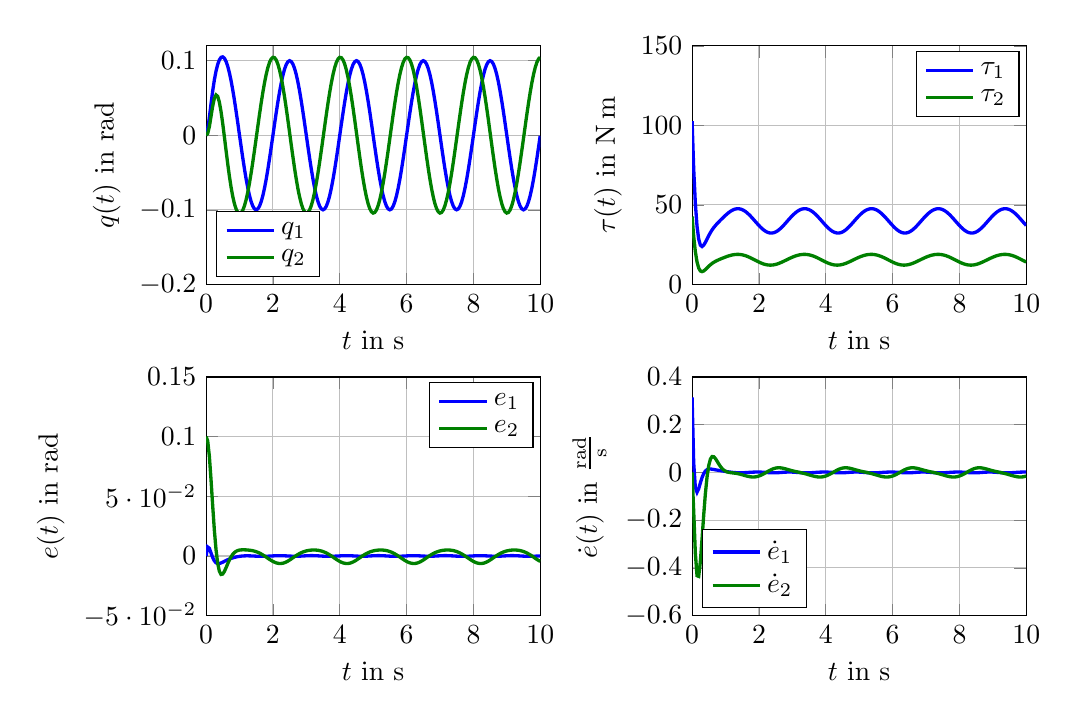
\begin{tikzpicture}

\begin{axis}[%
width=0.35\textwidth,
height=0.25\textwidth,
scale only axis,
xmin=0,
xmax=10,
xlabel={$t$ in $\mathrm{s}$},
xmajorgrids,
ymin=-0.2,
ymax=0.12,
ylabel={$q(t)$ in $\mathrm{rad}$},
ymajorgrids,
name=plot1,
legend style={at={(0.03,0.03)},anchor=south west,draw=black,fill=white,legend cell align=left}
]
\addplot [
color=blue,
solid,
line width=1.2pt
]
table[row sep=crcr]{
0 0\\
0.0477345288225563 0.00739832961256024\\
0.0977345288225563 0.0237707498973787\\
0.147734528822556 0.0421989570398354\\
0.197734528822556 0.0594828408218079\\
0.247734528822556 0.0742935678369579\\
0.297734528822556 0.0861906104293437\\
0.347734528822557 0.0951232357833952\\
0.397734528822557 0.101185320695722\\
0.447734528822557 0.104502663847835\\
0.497734528822557 0.105191844025\\
0.547734528822557 0.103356994077342\\
0.597734528822557 0.0991035459570871\\
0.647734528822557 0.0925558745818677\\
0.697734528822557 0.0838717981989785\\
0.747734528822557 0.0732512529990927\\
0.797734528822557 0.0609390578237993\\
0.847734528822557 0.0472228427410977\\
0.897734528822557 0.0324274780640394\\
0.947734528822557 0.016907189268258\\
0.997734528822557 0.00103627779601936\\
1.04773452882255 -0.014800874524872\\
1.09773452882255 -0.0302200193673153\\
1.14773452882254 -0.0448470977681129\\
1.19773452882254 -0.058327842866237\\
1.24773452882253 -0.0703366911966022\\
1.29773452882252 -0.0805848073181362\\
1.34773452882252 -0.088827061898667\\
1.39773452882251 -0.0948678339800026\\
1.44773452882251 -0.0985655358462681\\
1.4977345288225 -0.0998357853446554\\
1.5477345288225 -0.09865317722841\\
1.59773452882249 -0.0950516332932449\\
1.64773452882249 -0.0891233411679678\\
1.69773452882248 -0.0810163230532607\\
1.74773452882247 -0.0709307071340047\\
1.79773452882247 -0.0591138040741564\\
1.84773452882246 -0.0458541172646324\\
1.89773452882246 -0.0314744371027083\\
1.94773452882245 -0.0163241859157694\\
1.99773452882245 -0.000771191149677646\\
2.04773452882244 0.0148069295493796\\
2.09773452882244 0.0300315862289241\\
2.14773452882243 0.0445320548532285\\
2.19773452882243 0.0579541590967228\\
2.24773452882242 0.0699686273936337\\
2.29773452882241 0.080278966526212\\
2.34773452882241 0.0886287016694883\\
2.3977345288224 0.0948078379379557\\
2.4477345288224 0.0986583980295544\\
2.49773452882239 0.100078884397351\\
2.54773452882239 0.0990275057160079\\
2.59773452882238 0.0955240032611807\\
2.64773452882238 0.0896499226253335\\
2.69773452882237 0.0815472086184337\\
2.74773452882236 0.0714150602490757\\
2.79773452882236 0.0595050650112219\\
2.84773452882235 0.0461147267060098\\
2.89773452882235 0.0315795938333845\\
2.94773452882234 0.0162642716463296\\
2.99773452882234 0.000552650196458016\\
3.04773452882233 -0.0151623003464145\\
3.09773452882233 -0.0304888242753242\\
3.14773452882232 -0.0450464507286286\\
3.19773452882232 -0.0584755660660286\\
3.24773452882231 -0.0704462583787418\\
3.2977345288223 -0.0806662462230807\\
3.3477345288223 -0.0888877406793328\\
3.39773452882229 -0.0949131214014515\\
3.44773452882229 -0.0985993346125014\\
3.49773452882228 -0.0998609460088285\\
3.54773452882228 -0.0986718062857362\\
3.59773452882227 -0.095065312962508\\
3.64773452882227 -0.0891332799689376\\
3.69773452882226 -0.0810234557361919\\
3.74773452882225 -0.0709357602293839\\
3.79773452882225 -0.0591173399466184\\
3.84773452882224 -0.0458565658078241\\
3.89773452882224 -0.0314761207561597\\
3.94773452882223 -0.0163253409602662\\
3.99773452882223 -0.000771986417566046\\
4.04773452882224 0.0148063763873577\\
4.09773452882226 0.0300311949734294\\
4.14773452882228 0.0445317718041969\\
4.19773452882229 0.0579539487086264\\
4.24773452882231 0.069968466252679\\
4.29773452882233 0.0802788392083876\\
4.34773452882234 0.0886285980017471\\
4.39773452882236 0.0948077512285931\\
4.44773452882238 0.0986583239236404\\
4.49773452882239 0.100078820115257\\
4.54773452882241 0.0990274495236557\\
4.59773452882243 0.0955239540876939\\
4.64773452882244 0.0896498797854772\\
4.69773452882246 0.0815471716182554\\
4.74773452882248 0.0714150286606575\\
4.79773452882249 0.0595050384033086\\
4.84773452882251 0.0461147046163823\\
4.89773452882253 0.0315795757688556\\
4.94773452882254 0.0162642570978436\\
4.99773452882256 0.000552638659613591\\
5.04773452882258 -0.0151623093518507\\
5.09773452882259 -0.0304888311903764\\
5.14773452882261 -0.0450464559457343\\
5.19773452882263 -0.0584755699250453\\
5.24773452882264 -0.0704462611672879\\
5.29773452882266 -0.0806662481799034\\
5.34773452882268 -0.0888877419994557\\
5.39773452882269 -0.0949131222420792\\
5.44773452882271 -0.0985993350989392\\
5.49773452882273 -0.0998609462399497\\
5.54773452882274 -0.0986718063387603\\
5.59773452882276 -0.0950653128970264\\
5.64773452882278 -0.0891332798302364\\
5.69773452882279 -0.0810234555579753\\
5.74773452882281 -0.0709357600360203\\
5.79773452882283 -0.0591173397550149\\
5.84773452882284 -0.0458565656290095\\
5.89773452882286 -0.0314761205966317\\
5.94773452882288 -0.0163253408231333\\
5.99773452882289 -0.000771986303503261\\
6.04773452882291 0.014806376479326\\
6.09773452882293 0.0300311950453059\\
6.14773452882294 0.0445317718585359\\
6.19773452882296 0.0579539487481837\\
6.24773452882298 0.0699684662801693\\
6.29773452882299 0.0802788392263278\\
6.34773452882301 0.0886285980123669\\
6.39773452882303 0.0948077512337944\\
6.44773452882304 0.0986583239249931\\
6.49773452882306 0.100078820114016\\
6.54773452882308 0.0990274495207937\\
6.59773452882309 0.0955239540839387\\
6.64773452882311 0.0896498797813532\\
6.69773452882313 0.0815471716141225\\
6.74773452882314 0.0714150286567476\\
6.79773452882316 0.0595050383997565\\
6.84773452882318 0.046114704613253\\
6.89773452882319 0.0315795757661655\\
6.94773452882321 0.0162642570955777\\
6.99773452882323 0.000552638657738469\\
7.04773452882324 -0.015162309353378\\
7.09773452882326 -0.0304888311916015\\
7.14773452882328 -0.0450464559467017\\
7.1977345288233 -0.0584755699257958\\
7.24773452882331 -0.0704462611678575\\
7.29773452882333 -0.0806662481803229\\
7.34773452882335 -0.088887741999751\\
7.39773452882336 -0.0949131222422714\\
7.44773452882338 -0.098599335099046\\
7.4977345288234 -0.0998609462399854\\
7.54773452882341 -0.0986718063387367\\
7.59773452882343 -0.0950653128969535\\
7.64773452882345 -0.0891332798301224\\
7.69773452882346 -0.0810234555578277\\
7.74773452882348 -0.0709357600358457\\
7.7977345288235 -0.0591173397548192\\
7.84773452882351 -0.0458565656287984\\
7.89773452882353 -0.0314761205964108\\
7.94773452882355 -0.0163253408229077\\
7.99773452882356 -0.000771986303278147\\
8.04773452882354 0.014806376479545\\
8.09773452882351 0.0300311950455112\\
8.14773452882348 0.0445317718587197\\
8.19773452882345 0.0579539487483404\\
8.24773452882343 0.0699684662802955\\
8.2977345288234 0.0802788392264224\\
8.34773452882337 0.0886285980124305\\
8.39773452882334 0.0948077512338294\\
8.44773452882331 0.098658323925003\\
8.49773452882329 0.100078820114005\\
8.54773452882326 0.099027449520768\\
8.59773452882323 0.0955239540839032\\
8.6477345288232 0.0896498797813134\\
8.69773452882318 0.0815471716140837\\
8.74773452882315 0.0714150286567148\\
8.79773452882312 0.059505038399734\\
8.84773452882309 0.0461147046132443\\
8.89773452882307 0.0315795757661729\\
8.94773452882304 0.0162642570956027\\
8.99773452882301 0.000552638657781172\\
9.04773452882298 -0.0151623093533186\\
9.09773452882295 -0.0304888311915274\\
9.14773452882293 -0.0450464559466161\\
9.1977345288229 -0.0584755699257029\\
9.24773452882287 -0.070446261167762\\
9.29773452882284 -0.0806662481802302\\
9.34773452882282 -0.088887741999667\\
9.39773452882279 -0.094913122242202\\
9.44773452882276 -0.098599335098997\\
9.49773452882273 -0.0998609462399624\\
9.5477345288227 -0.0986718063387445\\
9.59773452882268 -0.0950653128969961\\
9.64773452882265 -0.089133279830203\\
9.69773452882262 -0.081023455557948\\
9.74773452882259 -0.0709357600360063\\
9.79773452882257 -0.0591173397550191\\
9.84773452882254 -0.0458565656290355\\
9.89773452882251 -0.0314761205966811\\
9.94773452882248 -0.0163253408232062\\
9.99773452882246 -0.000771986303598072\\
};
\addlegendentry{$q_1$};

\addplot [
color=green!50!black,
solid,
line width=1.2pt
]
table[row sep=crcr]{
0 0\\
0.0477345288225563 0.00237255990776453\\
0.0977345288225563 0.0115779540900686\\
0.147734528822556 0.025371859505962\\
0.197734528822556 0.0393040568364071\\
0.247734528822556 0.0496194124844249\\
0.297734528822556 0.0541487623938208\\
0.347734528822557 0.0522513838561907\\
0.397734528822557 0.0444118648367406\\
0.447734528822557 0.0317873463986827\\
0.497734528822557 0.0158257703954447\\
0.547734528822557 -0.00200909145564691\\
0.597734528822557 -0.0204074215076243\\
0.647734528822557 -0.0382957143611852\\
0.697734528822557 -0.0548556043102295\\
0.747734528822557 -0.0695031894913452\\
0.797734528822557 -0.0818491754975835\\
0.847734528822557 -0.0916545936490702\\
0.897734528822557 -0.0987911225882266\\
0.947734528822557 -0.10321025680787\\
0.997734528822557 -0.104922169272594\\
1.04773452882255 -0.103983081746663\\
1.09773452882255 -0.100489016398355\\
1.14773452882254 -0.094573616442908\\
1.19773452882254 -0.0864079818477484\\
1.24773452882253 -0.0762009291589805\\
1.29773452882252 -0.0641985910706028\\
1.34773452882252 -0.0506827278740655\\
1.39773452882251 -0.0359674864742414\\
1.44773452882251 -0.0203946036938737\\
1.4977345288225 -0.00432721864492711\\
1.5477345288225 0.0118574476376078\\
1.59773452882249 0.0277762477140239\\
1.64773452882249 0.0430487962987572\\
1.69773452882248 0.0573064042637011\\
1.74773452882247 0.0702009923731629\\
1.79773452882247 0.0814137408956296\\
1.84773452882246 0.0906632495836835\\
1.89773452882246 0.0977129969676267\\
1.94773452882245 0.102377900086109\\
1.99773452882245 0.104529788065832\\
2.04773452882244 0.104101617439807\\
2.09773452882244 0.101090274840696\\
2.14773452882243 0.0955578337073226\\
2.19773452882243 0.0876311553439511\\
2.24773452882242 0.0774997510701344\\
2.29773452882241 0.0654118530900178\\
2.34773452882241 0.0516686814443655\\
2.3977345288224 0.0366169493727561\\
2.4477345288224 0.0206397256875464\\
2.49773452882239 0.00414587217988175\\
2.54773452882239 -0.0124416098976152\\
2.59773452882238 -0.0286978744552514\\
2.64773452882238 -0.0442086257194806\\
2.69773452882237 -0.0585820330902308\\
2.74773452882236 -0.0714596119424589\\
2.79773452882236 -0.082525611659058\\
2.84773452882235 -0.091514598233503\\
2.89773452882235 -0.0982170864969212\\
2.94773452882234 -0.102483234259762\\
2.99773452882234 -0.104224731938742\\
3.04773452882233 -0.103415093539508\\
3.09773452882233 -0.100088578385808\\
3.14773452882232 -0.0943379579431511\\
3.19773452882232 -0.0863113036764999\\
3.24773452882231 -0.0762079255004094\\
3.2977345288223 -0.0642735483185844\\
3.3477345288223 -0.0507947841177551\\
3.39773452882229 -0.0360929422251354\\
3.44773452882229 -0.0205172201916563\\
3.49773452882228 -0.00443732955663439\\
3.54773452882228 0.0117643693125787\\
3.59773452882227 0.0277011248598949\\
3.64773452882227 0.042990320686442\\
3.69773452882226 0.0572621228320464\\
3.74773452882225 0.0701680791654606\\
3.79773452882225 0.0813894850202298\\
3.84773452882224 0.0906453170229789\\
3.89773452882224 0.0976995304854989\\
3.94773452882223 0.102367515478562\\
3.99773452882223 0.10452151322139\\
4.04773452882224 0.104094807606\\
4.09773452882226 0.101084525694985\\
4.14773452882228 0.0955529044396009\\
4.19773452882229 0.0876269071878015\\
4.24773452882231 0.0774961022886802\\
4.29773452882233 0.0654087488445331\\
4.34773452882234 0.0516660757402025\\
4.39773452882236 0.0366147959406458\\
4.44773452882238 0.0206379748654842\\
4.49773452882239 0.0041444713516212\\
4.54773452882241 -0.0124427141566067\\
4.59773452882243 -0.0286987337903645\\
4.64773452882244 -0.0442092877296181\\
4.69773452882246 -0.0585825397477383\\
4.74773452882248 -0.0714599987894342\\
4.79773452882249 -0.0825259076970228\\
4.84773452882251 -0.0915148263375647\\
4.89773452882253 -0.0982172641625488\\
4.94773452882254 -0.102483374507327\\
4.99773452882256 -0.104224844238684\\
5.04773452882258 -0.103415184664908\\
5.09773452882259 -0.100088653139896\\
5.14773452882261 -0.0943380197419561\\
5.19773452882263 -0.0863113549898172\\
5.24773452882264 -0.0762079681681438\\
5.29773452882266 -0.0642735837659934\\
5.34773452882268 -0.0507948134942512\\
5.39773452882269 -0.0360929664890879\\
5.44773452882271 -0.020517240159678\\
5.49773452882273 -0.00443734593135862\\
5.54773452882274 0.0117643559264607\\
5.59773452882276 0.0277011139451149\\
5.64773452882278 0.0429903118046323\\
5.69773452882279 0.0572621156155521\\
5.74773452882281 0.0701680733089735\\
5.79773452882283 0.0813894802723362\\
5.84773452882284 0.0906453131779455\\
5.89773452882286 0.0976995273756385\\
5.94773452882288 0.102367512967428\\
5.99773452882289 0.104521511197926\\
6.04773452882291 0.104094805979663\\
6.09773452882293 0.101084524391777\\
6.14773452882294 0.0955529033988882\\
6.19773452882296 0.0876269063598044\\
6.24773452882298 0.0774961016324901\\
6.29773452882299 0.0654087483265448\\
6.34773452882301 0.0516660753328615\\
6.39773452882303 0.0366147956214339\\
6.44773452882304 0.020637974616084\\
6.49773452882306 0.00414447115721847\\
6.54773452882308 -0.0124427143079137\\
6.59773452882309 -0.0286987339080679\\
6.64773452882311 -0.0442092878212308\\
6.69773452882313 -0.0585825398191609\\
6.74773452882314 -0.0714599988452667\\
6.79773452882316 -0.0825259077408264\\
6.84773452882318 -0.0915148263720803\\
6.89773452882319 -0.098217264189876\\
6.94773452882321 -0.102483374529069\\
6.99773452882323 -0.104224844256065\\
7.04773452882324 -0.103415184678861\\
7.09773452882326 -0.100088653151138\\
7.14773452882328 -0.0943380197510388\\
7.1977345288233 -0.086311354997169\\
7.24773452882331 -0.0762079681741001\\
7.29773452882333 -0.0642735837708193\\
7.34773452882335 -0.0507948134981585\\
7.39773452882336 -0.0360929664922469\\
7.44773452882338 -0.0205172401622269\\
7.4977345288234 -0.00443734593341051\\
7.54773452882341 0.011764355924813\\
7.59773452882343 0.0277011139437946\\
7.64773452882345 0.0429903118035759\\
7.69773452882346 0.0572621156147067\\
7.74773452882348 0.0701680733082951\\
7.7977345288235 0.0813894802717882\\
7.84773452882351 0.0906453131774974\\
7.89773452882353 0.0976995273752649\\
7.94773452882355 0.102367512967108\\
7.99773452882356 0.104521511197644\\
8.04773452882354 0.104094805979405\\
8.09773452882351 0.101084524391535\\
8.14773452882348 0.095552903398658\\
8.19773452882345 0.0876269063595832\\
8.24773452882343 0.077496101632277\\
8.2977345288234 0.0654087483263403\\
8.34773452882337 0.0516660753326679\\
8.39773452882334 0.0366147956212542\\
8.44773452882331 0.0206379746159217\\
8.49773452882329 0.00414447115707696\\
8.54773452882326 -0.0124427143080317\\
8.59773452882323 -0.0286987339081608\\
8.6477345288232 -0.044209287821298\\
8.69773452882318 -0.0585825398192033\\
8.74773452882315 -0.0714599988452863\\
8.79773452882312 -0.0825259077408265\\
8.84773452882309 -0.0915148263720652\\
8.89773452882307 -0.0982172641898506\\
8.94773452882304 -0.102483374529039\\
8.99773452882301 -0.104224844256035\\
9.04773452882298 -0.103415184678838\\
9.09773452882295 -0.100088653151126\\
9.14773452882293 -0.0943380197510437\\
9.1977345288229 -0.0863113549971943\\
9.24773452882287 -0.076207968174149\\
9.29773452882284 -0.064273583770894\\
9.34773452882282 -0.0507948134982599\\
9.39773452882279 -0.0360929664923748\\
9.44773452882276 -0.0205172401623798\\
9.49773452882273 -0.00443734593358559\\
9.5477345288227 0.0117643559246197\\
9.59773452882268 0.0277011139435882\\
9.64773452882265 0.0429903118033627\\
9.69773452882262 0.0572621156144935\\
9.74773452882259 0.0701680733080896\\
9.79773452882257 0.0813894802715985\\
9.84773452882254 0.0906453131773316\\
9.89773452882251 0.0976995273751313\\
9.94773452882248 0.102367512967014\\
9.99773452882246 0.104521511197596\\
};
\addlegendentry{$q_2$};

\end{axis}

\begin{axis}[%
width=0.35\textwidth,
height=0.25\textwidth,
scale only axis,
xmin=0,
xmax=10,
xlabel={$t$ in $\mathrm{s}$},
xmajorgrids,
ymin=-0.05,
ymax=0.15,
ylabel={$e(t)$ in $\mathrm{rad}$},
ymajorgrids,
name=plot3,
at=(plot1.below south west),
anchor=above north west,
legend style={draw=black,fill=white,legend cell align=left}
]
\addplot [
color=blue,
solid,
line width=1.2pt
]
table[row sep=crcr]{
0 0\\
0.0477345288225563 0.0075417703015502\\
0.0977345288225563 0.00645328783981116\\
0.147734528822556 0.00256480240351383\\
0.197734528822556 -0.00128159199219462\\
0.247734528822556 -0.00408793752613629\\
0.297734528822556 -0.00570929425469478\\
0.347734528822557 -0.00634795085131359\\
0.397734528822557 -0.00630200914951436\\
0.447734528822557 -0.00584766771742666\\
0.497734528822557 -0.00519437673228128\\
0.547734528822557 -0.00447932513962671\\
0.597734528822557 -0.00378037173979133\\
0.647734528822557 -0.00313436799369873\\
0.697734528822557 -0.00255381350510267\\
0.747734528822557 -0.00203910886159162\\
0.797734528822557 -0.00158623357089469\\
0.847734528822557 -0.00119080188662641\\
0.897734528822557 -0.000849682225423275\\
0.947734528822557 -0.000561188579739753\\
0.997734528822557 -0.000324565043816374\\
1.04773452882255 -0.000139225389237014\\
1.09773452882255 -4.01836987150642e-06\\
1.14773452882254 8.33383247680272e-05\\
1.19773452882254 0.000126594036629131\\
1.24773452882253 0.000131060885786516\\
1.29773452882252 0.000103491143493228\\
1.34773452882252 5.1776966590894e-05\\
1.39773452882251 -1.54775662006279e-05\\
1.44773452882251 -8.94602841380598e-05\\
1.4977345288225 -0.000161681948063208\\
1.5477345288225 -0.000224491709307981\\
1.59773452882249 -0.000271540924057026\\
1.64773452882249 -0.000298165420211244\\
1.69773452882248 -0.000301661640629197\\
1.74773452882247 -0.000281437003514504\\
1.79773452882247 -0.00023902017877038\\
1.84773452882246 -0.000177923589864827\\
1.89773452882246 -0.000103358735937212\\
1.94773452882245 -2.18147727810807e-05\\
1.99773452882245 5.94783974401463e-05\\
2.04773452882244 0.000133170364695264\\
2.09773452882244 0.000192451508229823\\
2.14773452882243 0.000231704590085514\\
2.19773452882243 0.000247089732857031\\
2.24773452882242 0.000237002917157378\\
2.29773452882241 0.000202349648410385\\
2.34773452882241 0.000146583262571914\\
2.3977345288224 7.54736082366342e-05\\
2.4477345288224 -3.40189915380706e-06\\
2.49773452882239 -8.14171046324697e-05\\
2.54773452882239 -0.000149836778284854\\
2.59773452882238 -0.000200829043868353\\
2.64773452882238 -0.000228416037139009\\
2.69773452882237 -0.000229223924523778\\
2.74773452882236 -0.000202916111532211\\
2.79773452882236 -0.000152240758267398\\
2.84773452882235 -8.26858514817452e-05\\
2.89773452882235 -1.79799470621106e-06\\
2.94773452882234 8.17290422550111e-05\\
2.99773452882234 0.000159062555813957\\
3.04773452882233 0.000222200432373913\\
3.09773452882233 0.000264786538203315\\
3.14773452882232 0.000282691285345513\\
3.19773452882232 0.000274317236476938\\
3.24773452882231 0.00024062806797541\\
3.2977345288223 0.000184930048478818\\
3.3477345288223 0.000112455747288465\\
3.39773452882229 2.98098552700826e-05\\
3.44773452882229 -5.56615178935321e-05\\
3.49773452882228 -0.000136521283889565\\
3.54773452882228 -0.000205862651992086\\
3.59773452882227 -0.000257861254814903\\
3.64773452882227 -0.000288226619272275\\
3.69773452882226 -0.000294528957738238\\
3.74773452882225 -0.000276383908183922\\
3.79773452882225 -0.000235484306364005\\
3.84773452882224 -0.000175475046734506\\
3.89773452882224 -0.000101675082551482\\
3.94773452882223 -2.06597283525997e-05\\
3.99773452882223 6.02736652594228e-05\\
4.04773452882224 0.000133723526655279\\
4.09773452882226 0.00019284276367151\\
4.14773452882228 0.000231987639073609\\
4.19773452882229 0.000247300120919496\\
4.24773452882231 0.000237164058087325\\
4.29773452882233 0.000202476966218418\\
4.34773452882234 0.000146686930303633\\
4.39773452882236 7.55603175948971e-05\\
4.44773452882238 -3.32779324094257e-06\\
4.49773452882239 -8.13528225382248e-05\\
4.54773452882241 -0.000149780585933693\\
4.59773452882243 -0.000200779870385831\\
4.64773452882244 -0.000228373197292284\\
4.69773452882246 -0.000229186924361829\\
4.74773452882248 -0.000202884523138741\\
4.79773452882249 -0.000152214150387929\\
4.84773452882251 -8.26637618979789e-05\\
4.89773452882253 -1.77993023047635e-06\\
4.94773452882254 8.17435906788622e-05\\
4.99773452882256 0.00015907409258842\\
5.04773452882258 0.000222209437733932\\
5.09773452882259 0.000264793453175451\\
5.14773452882261 0.000282696502369735\\
5.19773452882263 0.000274321095414032\\
5.24773452882264 0.000240630856446655\\
5.29773452882266 0.000184932005235158\\
5.34773452882268 0.000112457067356631\\
5.39773452882269 2.98106958580568e-05\\
5.44773452882271 -5.56610314774719e-05\\
5.49773452882273 -0.000136521052769359\\
5.54773452882274 -0.000205862598946047\\
5.59773452882276 -0.000257861320250047\\
5.64773452882278 -0.00028822675790155\\
5.69773452882279 -0.000294529135857244\\
5.74773452882281 -0.000276384101424748\\
5.79773452882283 -0.000235484497821466\\
5.84773452882284 -0.000175475225381708\\
5.89773452882286 -0.000101675241893938\\
5.94773452882288 -2.06598652855543e-05\\
5.99773452882289 6.02735514060411e-05\\
6.04773452882291 0.000133723434894635\\
6.09773452882293 0.000192842691994918\\
6.14773452882294 0.000231987584922384\\
6.19773452882296 0.000247300081532793\\
6.24773452882298 0.00023716403074657\\
6.29773452882299 0.000202476948402613\\
6.34773452882301 0.000146686919780439\\
6.39773452882303 7.55603124597409e-05\\
6.44773452882304 -3.32779455937404e-06\\
6.49773452882306 -8.13528212958853e-05\\
6.54773452882308 -0.000149780583103012\\
6.59773452882309 -0.000200779866693965\\
6.64773452882311 -0.000228373193262146\\
6.69773452882313 -0.000229186920351135\\
6.74773452882314 -0.000202884519376043\\
6.79773452882316 -0.000152214147004809\\
6.84773452882318 -8.26637589548818e-05\\
6.89773452882319 -1.77992773960078e-06\\
6.94773452882321 8.1743592737743e-05\\
6.99773452882323 0.000159074094253606\\
7.04773452882324 0.000222209439053773\\
7.09773452882326 0.000264793454200433\\
7.14773452882328 0.000282696503149708\\
7.1977345288233 0.000274321095993839\\
7.24773452882331 0.000240630856867041\\
7.29773452882333 0.000184932005530089\\
7.34773452882335 0.00011245706755543\\
7.39773452882336 2.98106959840394e-05\\
7.44773452882338 -5.56610314049327e-05\\
7.4977345288234 -0.000136521052735206\\
7.54773452882341 -0.000205862598938358\\
7.59773452882343 -0.000257861320259484\\
7.64773452882345 -0.000288226757921686\\
7.69773452882346 -0.00029452913588264\\
7.74773452882348 -0.000276384101452282\\
7.7977345288235 -0.000235484497848215\\
7.84773452882351 -0.000175475225406695\\
7.89773452882353 -0.000101675241915677\\
7.94773452882355 -2.06598653043448e-05\\
7.99773452882356 6.02735513908619e-05\\
8.04773452882354 0.000133723434869847\\
8.09773452882351 0.000192842691963738\\
8.14773452882348 0.000231987584889085\\
8.19773452882345 0.000247300081501679\\
8.24773452882343 0.000237164030720508\\
8.2977345288234 0.000202476948383365\\
8.34773452882337 0.000146686919768671\\
8.39773452882334 7.55603124559384e-05\\
8.44773452882331 -3.32779455537724e-06\\
8.49773452882329 -8.13528212848941e-05\\
8.54773452882326 -0.000149780583085804\\
8.59773452882323 -0.000200779866671469\\
8.6477345288232 -0.000228373193235362\\
8.69773452882318 -0.000229186920321048\\
8.74773452882315 -0.000202884519344027\\
8.79773452882312 -0.000152214146971738\\
8.84773452882309 -8.26637589224563e-05\\
8.89773452882307 -1.77992770827168e-06\\
8.94773452882304 8.17435927667649e-05\\
8.99773452882301 0.000159074094279848\\
9.04773452882298 0.000222209439075853\\
9.09773452882295 0.000264793454218488\\
9.14773452882293 0.000282696503162962\\
9.1977345288229 0.000274321096002304\\
9.24773452882287 0.000240630856869928\\
9.29773452882284 0.000184932005527827\\
9.34773452882282 0.000112457067547936\\
9.39773452882279 2.98106959716465e-05\\
9.44773452882276 -5.56610314221412e-05\\
9.49773452882273 -0.000136521052756702\\
9.5477345288227 -0.000205862598963699\\
9.59773452882268 -0.000257861320288294\\
9.64773452882265 -0.000288226757952925\\
9.69773452882262 -0.000294529135915975\\
9.74773452882259 -0.000276384101486768\\
9.79773452882257 -0.000235484497883298\\
9.84773452882254 -0.000175475225440869\\
9.89773452882251 -0.000101675241948707\\
9.94773452882248 -2.06598653350668e-05\\
9.99773452882246 6.02735513629604e-05\\
};
\addlegendentry{$e_1$};

\addplot [
color=green!50!black,
solid,
line width=1.2pt
]
table[row sep=crcr]{
0 0.1\\
0.0477345288225563 0.0965051090299506\\
0.0977345288225563 0.0837452201272272\\
0.147734528822556 0.064049647082207\\
0.197734528822556 0.0420139278574688\\
0.247734528822556 0.0215927316530763\\
0.297734528822556 0.00520406185908398\\
0.347734528822557 -0.00621934300171928\\
0.397734528822557 -0.0128340689981244\\
0.447734528822557 -0.0154413457101644\\
0.497734528822557 -0.0151140576432416\\
0.547734528822557 -0.0129310084584636\\
0.597734528822557 -0.00981661622956569\\
0.647734528822557 -0.00646804508216417\\
0.697734528822557 -0.00334564451938391\\
0.747734528822557 -0.000702440819476513\\
0.797734528822557 0.00136785932293448\\
0.847734528822557 0.00287930871698856\\
0.897734528822557 0.00390781104201909\\
0.947734528822557 0.00455526067746077\\
0.997734528822557 0.00492470197987489\\
1.04773452882255 0.00510541280894768\\
1.09773452882255 0.00516584218105806\\
1.14773452882254 0.00515210985473676\\
1.19773452882254 0.00508999715386867\\
1.24773452882253 0.00498878502147347\\
1.29773452882252 0.00484576681768991\\
1.34773452882252 0.00465068701958356\\
1.39773452882251 0.00438969063561231\\
1.44773452882251 0.00404860300534023\\
1.4977345288225 0.00361550589270693\\
1.5477345288225 0.00308265227648407\\
1.59773452882249 0.00244779002314641\\
1.64773452882249 0.00171496314457216\\
1.69773452882248 0.000894844565892755\\
1.74773452882247 4.6379376404948e-06\\
1.79773452882247 -0.000932424720996985\\
1.84773452882246 -0.00188796465161528\\
1.89773452882246 -0.00282968542142896\\
1.94773452882245 -0.00372290395570557\\
1.99773452882245 -0.00453232077311316\\
2.04773452882244 -0.00522394850208691\\
2.09773452882244 -0.00576710062338871\\
2.14773452882243 -0.00613632711913584\\
2.19773452882243 -0.00631317065005119\\
2.24773452882242 -0.00628760693260309\\
2.29773452882241 -0.00605902883707713\\
2.34773452882241 -0.00563664058985293\\
2.3977345288224 -0.00503915353409424\\
2.4477345288224 -0.0042937249989789\\
2.49773452882239 -0.00343415942762702\\
2.54773452882239 -0.00249849001644262\\
2.59773452882238 -0.00152616328188607\\
2.64773452882238 -0.000555133723817845\\
2.69773452882237 0.000380784260665061\\
2.74773452882236 0.00125398163168013\\
2.79773452882236 0.0020442954844458\\
2.84773452882235 0.00273931330145075\\
2.89773452882235 0.00333377495073432\\
2.94773452882234 0.00382823812936405\\
2.99773452882234 0.00422726464602369\\
3.04773452882233 0.00453742460178208\\
3.09773452882233 0.00476540416849022\\
3.14773452882232 0.00491645135494896\\
3.19773452882232 0.00499331898257986\\
3.24773452882231 0.00499578136285367\\
3.2977345288223 0.00492072406561585\\
3.3477345288223 0.00476274326321174\\
3.39773452882229 0.00451514638644072\\
3.44773452882229 0.00417121950305466\\
3.49773452882228 0.003725616804345\\
3.54773452882228 0.00317573060144482\\
3.59773452882227 0.00252291287720958\\
3.64773452882227 0.00177343875682565\\
3.69773452882226 0.000939125997491123\\
3.74773452882225 3.75511452934962e-05\\
3.79773452882225 -0.000908168845638185\\
3.84773452882224 -0.00187003209094254\\
3.89773452882224 -0.00281621893932302\\
3.94773452882223 -0.00371251934816971\\
3.99773452882223 -0.00452404592867205\\
4.04773452882224 -0.00521713866826971\\
4.09773452882226 -0.00576135147766092\\
4.14773452882228 -0.00613139785139243\\
4.19773452882229 -0.00630892249387735\\
4.24773452882231 -0.00628395815112451\\
4.29773452882233 -0.00605592459157027\\
4.34773452882234 -0.00563403488567163\\
4.39773452882236 -0.00503700010197102\\
4.44773452882238 -0.00429197417691006\\
4.49773452882239 -0.00343275859936679\\
4.54773452882241 -0.00249738575745827\\
4.59773452882243 -0.00152530394678651\\
4.64773452882244 -0.000554471713699399\\
4.69773452882246 0.000381290918149639\\
4.74773452882248 0.00125436847863047\\
4.79773452882249 0.00204459152238566\\
4.84773452882251 0.00273954140548979\\
4.89773452882253 0.00333395261634431\\
4.94773452882254 0.00382837837691878\\
4.99773452882256 0.00422737694596567\\
5.04773452882258 0.00453751572719344\\
5.09773452882259 0.00476547892260341\\
5.14773452882261 0.00491651315379468\\
5.19773452882263 0.00499337029595412\\
5.24773452882264 0.00499582403066197\\
5.29773452882266 0.00492075951311487\\
5.34773452882268 0.00476277263981349\\
5.39773452882269 0.00451517065051258\\
5.44773452882271 0.00417123947120744\\
5.49773452882273 0.00372563317920901\\
5.54773452882274 0.00317574398770813\\
5.59773452882276 0.00252292379213605\\
5.64773452882278 0.00177344763877906\\
5.69773452882279 0.000939133214121791\\
5.74773452882281 3.75570019050253e-05\\
5.79773452882283 -0.000908164097636874\\
5.84773452882284 -0.00187002824582229\\
5.89773452882286 -0.00281621582940085\\
5.94773452882288 -0.0037125168370024\\
5.99773452882289 -0.00452404390520668\\
6.04773452882291 -0.00521713704196468\\
6.09773452882293 -0.00576135017451614\\
6.14773452882294 -0.00613139681077367\\
6.19773452882296 -0.00630892166600239\\
6.24773452882298 -0.00628395749508183\\
6.29773452882299 -0.00605592407375061\\
6.34773452882301 -0.00563403447851686\\
6.39773452882303 -0.00503699978295795\\
6.44773452882304 -0.00429197392771682\\
6.49773452882306 -0.00343275840517364\\
6.54773452882308 -0.00249738560635874\\
6.59773452882309 -0.00152530382928292\\
6.64773452882311 -0.000554471622274316\\
6.69773452882313 0.000381290989401525\\
6.74773452882314 0.00125436853431352\\
6.79773452882316 0.00204459156606462\\
6.84773452882318 0.0027395414399089\\
6.89773452882319 0.00333395264360517\\
6.94773452882321 0.00382837839862669\\
6.99773452882323 0.00422737696334478\\
7.04773452882324 0.00453751574117811\\
7.09773452882326 0.00476547893390898\\
7.14773452882328 0.00491651316297125\\
7.1977345288233 0.00499337030342811\\
7.24773452882331 0.00499582403676538\\
7.29773452882333 0.00492075951810979\\
7.34773452882335 0.00476277264390683\\
7.39773452882336 0.00451517065387077\\
7.44773452882338 0.00417123947396314\\
7.4977345288234 0.00372563318147083\\
7.54773452882341 0.00317574398956307\\
7.59773452882343 0.00252292379365643\\
7.64773452882345 0.00177344764002287\\
7.69773452882346 0.000939133215137875\\
7.74773452882348 3.75570027326688e-05\\
7.7977345288235 -0.000908164096964231\\
7.84773452882351 -0.00187002824527768\\
7.89773452882353 -0.00281621582896101\\
7.94773452882355 -0.00371251683664849\\
7.99773452882356 -0.00452404390492252\\
8.04773452882354 -0.00521713704173565\\
8.09773452882351 -0.00576135017432942\\
8.14773452882348 -0.00613139681061887\\
8.19773452882345 -0.00630892166587112\\
8.24773452882343 -0.00628395749496743\\
8.2977345288234 -0.00605592407364824\\
8.34773452882337 -0.00563403447842321\\
8.39773452882334 -0.00503699978287198\\
8.44773452882331 -0.00429197392763832\\
8.49773452882329 -0.00343275840510317\\
8.54773452882326 -0.00249738560629687\\
8.59773452882323 -0.001525303829231\\
8.6477345288232 -0.000554471622233141\\
8.69773452882318 0.000381290989431772\\
8.74773452882315 0.00125436853433242\\
8.79773452882312 0.0020445915660726\\
8.84773452882309 0.00273954143990604\\
8.89773452882307 0.00333395264359265\\
8.94773452882304 0.00382837839860531\\
8.99773452882301 0.00422737696331574\\
9.04773452882298 0.00453751574114269\\
9.09773452882295 0.00476547893386832\\
9.14773452882293 0.00491651316292668\\
9.1977345288229 0.00499337030338083\\
9.24773452882287 0.00499582403671726\\
9.29773452882284 0.00492075951806178\\
9.34773452882282 0.00476277264386063\\
9.39773452882279 0.00451517065382737\\
9.44773452882276 0.00417123947392462\\
9.49773452882273 0.0037256331814377\\
9.5477345288227 0.0031757439895368\\
9.59773452882268 0.00252292379363758\\
9.64773452882265 0.00177344764001279\\
9.69773452882262 0.000939133215136403\\
9.74773452882259 3.75570027402738e-05\\
9.79773452882257 -0.000908164096947842\\
9.84773452882254 -0.00187002824525258\\
9.89773452882251 -0.0028162158289283\\
9.94773452882248 -0.003712516836609\\
9.99773452882246 -0.00452404390487772\\
};
\addlegendentry{$e_2$};

\end{axis}

\begin{axis}[%
width=0.35\textwidth,
height=0.25\textwidth,
scale only axis,
xmin=0,
xmax=10,
xlabel={$t$ in $\mathrm{s}$},
xmajorgrids,
ymin=-0.6,
ymax=0.4,
ylabel={$\dot{e}(t)$ in $\mathrm{\frac{rad}{s}}$},
ymajorgrids,
name=plot2,
at=(plot3.right of south east),
anchor=left of south west,
legend style={at={(0.03,0.03)},anchor=south west,draw=black,fill=white,legend cell align=left}
]
\addplot [
color=blue,
solid,
line width=1.2pt
]
table[row sep=crcr]{
0 0.314159265358979\\
0.0477345288225563 0.0410521590188259\\
0.0977345288225563 -0.0637839900805432\\
0.147734528822556 -0.0828455280104373\\
0.197734528822556 -0.067951497395505\\
0.247734528822556 -0.043922301065197\\
0.297734528822556 -0.0216202551574273\\
0.347734528822557 -0.00488383981035356\\
0.397734528822557 0.00586599792768575\\
0.447734528822557 0.0116914551942529\\
0.497734528822557 0.0140728320699376\\
0.547734528822557 0.0143612525298783\\
0.597734528822557 0.0135628327509118\\
0.647734528822557 0.0123188062853489\\
0.697734528822557 0.0109776252936689\\
0.747734528822557 0.00969054197387342\\
0.797734528822557 0.00849546678226365\\
0.847734528822557 0.00737737918004511\\
0.897734528822557 0.00630605679914709\\
0.947734528822557 0.00525646012145203\\
0.997734528822557 0.00421749064295496\\
1.04773452882255 0.0031936576320854\\
1.09773452882255 0.0022027937157551\\
1.14773452882254 0.00127185135554814\\
1.19773452882254 0.000432062544261147\\
1.24773452882253 -0.000285732786816151\\
1.29773452882252 -0.000855095471464423\\
1.34773452882252 -0.00125706061294892\\
1.39773452882251 -0.00148217223236449\\
1.44773452882251 -0.00153149940263162\\
1.4977345288225 -0.00141673200111669\\
1.5477345288225 -0.00115948762748342\\
1.59773452882249 -0.000789960930616992\\
1.64773452882249 -0.000345030029973464\\
1.69773452882248 0.000134079980108198\\
1.74773452882247 0.00060447673008851\\
1.79773452882247 0.00102450598267312\\
1.84773452882246 0.00135673427042576\\
1.89773452882246 0.00157082612744824\\
1.94773452882245 0.00164610669881299\\
1.99773452882245 0.00157358930148344\\
2.04773452882244 0.00135725473898762\\
2.09773452882244 0.00101439380066448\\
2.14773452882243 0.000574863967302497\\
2.19773452882243 7.91658486101743e-05\\
2.24773452882242 -0.000424680303044322\\
2.29773452882241 -0.000885371763706455\\
2.34773452882241 -0.00125344036832556\\
2.3977345288224 -0.00148682702444018\\
2.4477345288224 -0.00155628703917184\\
2.49773452882239 -0.00144983598523703\\
2.54773452882239 -0.00117540106819106\\
2.59773452882238 -0.000760987400284865\\
2.64773452882238 -0.000252024627909408\\
2.69773452882237 0.000293927591377557\\
2.74773452882236 0.000814393993995965\\
2.79773452882236 0.00124998135662718\\
2.84773452882235 0.00155185934200047\\
2.89773452882235 0.00168755571703888\\
2.94773452882234 0.00164427188086125\\
2.99773452882234 0.00142942583966454\\
3.04773452882233 0.0010686226786118\\
3.09773452882233 0.00060162957528187\\
3.14773452882232 7.71375932333007e-05\\
3.19773452882232 -0.000452876533007296\\
3.24773452882231 -0.000938481930403551\\
3.2977345288223 -0.0013363001741859\\
3.3477345288223 -0.00161288282653332\\
3.39773452882229 -0.00174685115803387\\
3.44773452882229 -0.00172983839640499\\
3.49773452882228 -0.00156636777105676\\
3.54773452882228 -0.00127284068150884\\
3.59773452882227 -0.00087581229452964\\
3.64773452882227 -0.000409714670571798\\
3.69773452882226 8.58328143345244e-05\\
3.74773452882225 0.000568997125504095\\
3.79773452882225 0.000998857195267933\\
3.84773452882224 0.00133853286083885\\
3.89773452882224 0.00155814556848682\\
3.94773452882223 0.00163741886536117\\
3.99773452882223 0.00156771640174208\\
4.04773452882224 0.00135331941680561\\
4.09773452882226 0.00101176541757153\\
4.14773452882228 0.000573104357429188\\
4.19773452882229 7.79792106169741e-05\\
4.24773452882231 -0.000425489717839622\\
4.29773452882233 -0.000885932458679045\\
4.34773452882234 -0.00125383707773657\\
4.39773452882236 -0.00148711631603039\\
4.44773452882238 -0.00155650706242758\\
4.49773452882239 -0.00145001235273146\\
4.54773452882241 -0.00117555046708324\\
4.59773452882243 -0.000761120014116032\\
4.64773452882244 -0.000252145973974882\\
4.69773452882246 0.0002938151487685\\
4.74773452882248 0.000814289991091094\\
4.79773452882249 0.00124988625152073\\
4.84773452882251 0.00155177382364269\\
4.89773452882253 0.00168748028587146\\
4.94773452882254 0.00164420665422937\\
4.99773452882256 0.00142937051843867\\
5.04773452882258 0.00106857661088938\\
5.09773452882259 0.000601591863973405\\
5.14773452882261 7.7107210166294e-05\\
5.19773452882263 -0.00045290064832948\\
5.24773452882264 -0.000938500796979769\\
5.29773452882266 -0.00133631472201393\\
5.34773452882268 -0.00161289387213842\\
5.39773452882269 -0.00174685939770154\\
5.44773452882271 -0.00172984441141666\\
5.49773452882273 -0.00156637203978269\\
5.54773452882274 -0.00127284359429692\\
5.59773452882276 -0.000875814168534744\\
5.64773452882278 -0.000409715762888119\\
5.69773452882279 8.58322959197133e-05\\
5.74773452882281 0.000568997014085582\\
5.79773452882283 0.000998857358298855\\
5.84773452882284 0.0013385331949381\\
5.89773452882286 0.00155814599508375\\
5.94773452882288 0.00163741932681333\\
5.99773452882289 0.00156771685775325\\
6.04773452882291 0.00135331984110909\\
6.09773452882293 0.00101176579484197\\
6.14773452882294 0.000573104680530512\\
6.19773452882296 7.79794782704846e-05\\
6.24773452882298 -0.000425489502979687\\
6.29773452882299 -0.000885932291557312\\
6.34773452882301 -0.00125383695205164\\
6.39773452882303 -0.00148711622507608\\
6.44773452882304 -0.00155650699965721\\
6.49773452882306 -0.00145001231212426\\
6.54773452882308 -0.00117555044333673\\
6.59773452882309 -0.000761120002735344\\
6.64773452882311 -0.00025214597127185\\
6.69773452882313 0.000293815145720383\\
6.74773452882314 0.000814289984539862\\
6.79773452882316 0.00124988624312877\\
6.84773452882318 0.00155177381458899\\
6.89773452882319 0.00168748027694732\\
6.94773452882321 0.00164420664592746\\
6.99773452882323 0.00142937051102981\\
7.04773452882324 0.00106857660448623\\
7.09773452882326 0.00060159185858355\\
7.14773452882328 7.7107205730842e-05\\
7.1977345288233 -0.000452900651906063\\
7.24773452882331 -0.000938500799809394\\
7.29773452882333 -0.00133631472421192\\
7.34773452882335 -0.00161289387381144\\
7.39773452882336 -0.0017468593989494\\
7.44773452882338 -0.00172984441232204\\
7.4977345288234 -0.00156637204042028\\
7.54773452882341 -0.00127284359472512\\
7.59773452882343 -0.000875814168806333\\
7.64773452882345 -0.000409715763041524\\
7.69773452882346 8.58322958504354e-05\\
7.74773452882348 0.000568997014076006\\
7.7977345288235 0.000998857358327443\\
7.84773452882351 0.0013385331949905\\
7.89773452882353 0.00155814599514725\\
7.94773452882355 0.00163741932687989\\
7.99773452882356 0.00156771685781704\\
8.04773452882354 0.00135331984121212\\
8.09773452882351 0.00101176579502482\\
8.14773452882348 0.000573104680785197\\
8.19773452882345 7.79794785710775e-05\\
8.24773452882343 -0.00042548950266133\\
8.2977345288234 -0.000885932291245423\\
8.34773452882337 -0.00125383695176631\\
8.39773452882334 -0.00148711622483183\\
8.44773452882331 -0.00155650699946497\\
8.49773452882329 -0.00145001231198911\\
8.54773452882326 -0.0011755504432631\\
8.59773452882323 -0.000761120002724658\\
8.6477345288232 -0.000252145971323975\\
8.69773452882318 0.000293815145608362\\
8.74773452882315 0.000814289984371025\\
8.79773452882312 0.00124988624290862\\
8.84773452882309 0.00155177381432486\\
8.89773452882307 0.00168748027664678\\
8.94773452882304 0.00164420664559928\\
8.99773452882301 0.0014293705106827\\
9.04773452882298 0.00106857660413007\\
9.09773452882295 0.000601591858227446\\
9.14773452882293 7.71072053837307e-05\\
9.1977345288229 -0.0004529006522348\\
9.24773452882287 -0.000938500800112596\\
9.29773452882284 -0.00133631472448129\\
9.34773452882282 -0.00161289387404151\\
9.39773452882279 -0.0017468593991332\\
9.44773452882276 -0.00172984441245769\\
9.49773452882273 -0.00156637204050362\\
9.5477345288227 -0.00127284359475565\\
9.59773452882268 -0.000875814168780742\\
9.64773452882265 -0.000409715762962642\\
9.69773452882262 8.5832295981636e-05\\
9.74773452882259 0.000568997014256195\\
9.79773452882257 0.000998857358554095\\
9.84773452882254 0.00133853319525717\\
9.89773452882251 0.0015581459954484\\
9.94773452882248 0.00163741932720834\\
9.99773452882246 0.00156771685816531\\
};
\addlegendentry{$\dot{e}_1$};

\addplot [
color=green!50!black,
solid,
line width=1.2pt
]
table[row sep=crcr]{
0 -0\\
0.0477345288225563 -0.161513696285704\\
0.0977345288225563 -0.338935892061498\\
0.147734528822556 -0.432600881590098\\
0.197734528822556 -0.435323101052681\\
0.247734528822556 -0.373444097161478\\
0.297734528822556 -0.279082645627354\\
0.347734528822557 -0.178483639497766\\
0.397734528822557 -0.0888686198448159\\
0.447734528822557 -0.0190665594316132\\
0.497734528822557 0.0285168690529326\\
0.547734528822557 0.0556945263563498\\
0.597734528822557 0.0665359563815174\\
0.647734528822557 0.0658511244219005\\
0.697734528822557 0.0581741263435571\\
0.747734528822557 0.0472043284171031\\
0.797734528822557 0.0356055296372346\\
0.847734528822557 0.0250450073400084\\
0.897734528822557 0.0163643484573089\\
0.947734528822557 0.00979915189899337\\
0.997734528822557 0.00519331092115816\\
1.04773452882255 0.00217856573852814\\
1.09773452882255 0.000308479328005609\\
1.14773452882254 -0.000852243148841164\\
1.19773452882254 -0.00167594788453218\\
1.24773452882253 -0.0024483454313052\\
1.29773452882252 -0.00336377895735474\\
1.34773452882252 -0.00453180076139914\\
1.39773452882251 -0.00598938249185449\\
1.44773452882251 -0.00771500212100956\\
1.4977345288225 -0.00964245021567572\\
1.5477345288225 -0.0116733820378777\\
1.59773452882249 -0.0136884124394476\\
1.64773452882249 -0.0155569626110181\\
1.69773452882248 -0.017146201937221\\
1.74773452882247 -0.0183293734862054\\
1.79773452882247 -0.0189936342541532\\
1.84773452882246 -0.019047355313861\\
1.89773452882246 -0.018426666802834\\
1.94773452882245 -0.0171009281930295\\
1.99773452882245 -0.0150767612412266\\
2.04773452882244 -0.0124002883504196\\
2.09773452882244 -0.00915725098653521\\
2.14773452882243 -0.00547072369670407\\
2.19773452882243 -0.00149618840999929\\
2.24773452882242 0.00258618500804625\\
2.29773452882241 0.00658204647683458\\
2.34773452882241 0.0102958679883343\\
2.3977345288224 0.01354570734115\\
2.4477345288224 0.016178452977012\\
2.49773452882239 0.0180837456562635\\
2.54773452882239 0.0192044728939367\\
2.59773452882238 0.0195418579645888\\
2.64773452882238 0.0191538196491722\\
2.69773452882237 0.018146385999794\\
2.74773452882236 0.0166592451974839\\
2.79773452882236 0.0148476504950226\\
2.84773452882235 0.0128635464011444\\
2.89773452882235 0.0108387932134994\\
2.94773452882234 0.00887278524898101\\
2.99773452882234 0.00702579414908305\\
3.04773452882233 0.00531829712214037\\
3.09773452882233 0.00373561464513275\\
3.14773452882232 0.00223653606024288\\
3.19773452882232 0.000764303341552447\\
3.24773452882231 -0.00074168201094732\\
3.2977345288223 -0.00233484954641983\\
3.3477345288223 -0.00405223071847366\\
3.39773452882229 -0.0059077168387448\\
3.44773452882229 -0.00788815797109838\\
3.49773452882228 -0.00995236128602373\\
3.54773452882228 -0.0120328214706686\\
3.59773452882227 -0.0140398549475758\\
3.64773452882227 -0.015867701140545\\
3.69773452882226 -0.0174020835363539\\
3.74773452882225 -0.0185286800152888\\
3.79773452882225 -0.0191419308917608\\
3.84773452882224 -0.0191536144916295\\
3.89773452882224 -0.0185006459629032\\
3.94773452882223 -0.0171516050187619\\
3.99773452882223 -0.0151115664195263\\
4.04773452882224 -0.0124248813732752\\
4.09773452882226 -0.00917562517211029\\
4.14773452882228 -0.00548547917258591\\
4.19773452882229 -0.00150886247914669\\
4.24773452882231 0.00257479846805636\\
4.29773452882233 0.00657162506446607\\
4.34773452882234 0.0102863506387428\\
4.39773452882236 0.0135371462741108\\
4.44773452882238 0.0161709200304894\\
4.49773452882239 0.018077281667913\\
4.54773452882241 0.0191990680555458\\
4.59773452882243 0.0195374521173242\\
4.64773452882244 0.0191503134754414\\
4.69773452882246 0.0181436563992322\\
4.74773452882248 0.0166571603992285\\
4.79773452882249 0.0148460824017533\\
4.84773452882251 0.0128623791557269\\
4.89773452882253 0.0108379280001557\\
4.94773452882254 0.00887214193325139\\
4.99773452882256 0.00702531061237631\\
5.04773452882258 0.00531792716081291\\
5.09773452882259 0.00373532517833623\\
5.14773452882261 0.00223630420394996\\
5.19773452882263 0.000764113712949627\\
5.24773452882264 -0.000741839561971047\\
5.29773452882266 -0.00233498170965246\\
5.34773452882268 -0.00405234201656623\\
5.39773452882269 -0.00590781050765621\\
5.44773452882271 -0.00788823651541526\\
5.49773452882273 -0.00995242679829672\\
5.54773452882274 -0.0120328757935405\\
5.59773452882276 -0.0140398997413836\\
5.64773452882278 -0.015867737901719\\
5.69773452882279 -0.0174021135961884\\
5.74773452882281 -0.0185287045360046\\
5.79773452882283 -0.0191419508676991\\
5.84773452882284 -0.0191536307576216\\
5.89773452882286 -0.0185006592087505\\
5.94773452882288 -0.0171516158074847\\
5.99773452882289 -0.0151115752069731\\
6.04773452882291 -0.0124248885271212\\
6.09773452882293 -0.00917563098900673\\
6.14773452882294 -0.00548548389272455\\
6.19773452882296 -0.00150886629819175\\
6.24773452882298 0.00257479538957478\\
6.29773452882299 0.0065716225939253\\
6.34773452882301 0.0102863486659669\\
6.39773452882303 0.013537144707254\\
6.44773452882304 0.0161709187929185\\
6.49773452882306 0.0180772806957933\\
6.54773452882308 0.0191990672959204\\
6.59773452882309 0.0195374515265271\\
6.64773452882311 0.0191503130177486\\
6.69773452882313 0.0181436560456817\\
6.74773452882314 0.0166571601265723\\
6.79773452882316 0.0148460821915279\\
6.84773452882318 0.0128623789934233\\
6.89773452882319 0.0108379278744905\\
6.94773452882321 0.00887214183553775\\
6.99773452882323 0.00702531053598043\\
7.04773452882324 0.00531792710070849\\
7.09773452882326 0.00373532513073063\\
7.14773452882328 0.00223630416599052\\
7.1977345288233 0.000764113682488077\\
7.24773452882331 -0.000741839586556797\\
7.29773452882333 -0.00233498172959629\\
7.34773452882335 -0.00405234203281207\\
7.39773452882336 -0.00590781052093714\\
7.44773452882338 -0.00788823652630366\\
7.4977345288234 -0.0099524268072444\\
7.54773452882341 -0.0120328758009068\\
7.59773452882343 -0.0140398997474561\\
7.64773452882345 -0.0158677379067306\\
7.69773452882346 -0.0174021136003251\\
7.74773452882348 -0.0185287045394189\\
7.7977345288235 -0.0191419508705124\\
7.84773452882351 -0.0191536307599357\\
7.89773452882353 -0.0185006592106459\\
7.94773452882355 -0.0171516158090316\\
7.99773452882356 -0.0151115752082268\\
8.04773452882354 -0.0124248885281264\\
8.09773452882351 -0.00917563098982854\\
8.14773452882348 -0.00548548389339959\\
8.19773452882345 -0.00150886629875124\\
8.24773452882343 0.00257479538909736\\
8.2977345288234 0.00657162259349731\\
8.34773452882337 0.010286348665558\\
8.39773452882334 0.0135371447068427\\
8.44773452882331 0.0161709187924919\\
8.49773452882329 0.018077280695347\\
8.54773452882326 0.0191990672954571\\
8.59773452882323 0.0195374515260553\\
8.6477345288232 0.01915031301728\\
8.69773452882318 0.0181436560452292\\
8.74773452882315 0.016657160126149\\
8.79773452882312 0.0148460821911456\\
8.84773452882309 0.0128623789930909\\
8.89773452882307 0.0108379278742164\\
8.94773452882304 0.00887214183532647\\
8.99773452882301 0.00702531053583795\\
9.04773452882298 0.00531792710063411\\
9.09773452882295 0.00373532513072519\\
9.14773452882293 0.00223630416605156\\
9.1977345288229 0.000764113682615752\\
9.24773452882287 -0.000741839586368281\\
9.29773452882284 -0.00233498172935093\\
9.34773452882282 -0.00405234203251648\\
9.39773452882279 -0.0059078105205968\\
9.44773452882276 -0.00788823652592718\\
9.49773452882273 -0.00995242680684094\\
9.5477345288227 -0.0120328758004862\\
9.59773452882268 -0.0140398997470296\\
9.64773452882265 -0.0158677379063085\\
9.69773452882262 -0.0174021135999188\\
9.74773452882259 -0.0185287045390395\\
9.79773452882257 -0.0191419508701726\\
9.84773452882254 -0.0191536307596444\\
9.89773452882251 -0.0185006592104131\\
9.94773452882248 -0.0171516158088644\\
9.99773452882246 -0.0151115752081335\\
};
\addlegendentry{$\dot{e}_2$};

\end{axis}

\begin{axis}[%
width=0.35\textwidth,
height=0.25\textwidth,
scale only axis,
xmin=0,
xmax=10,
xlabel={$t$ in $\mathrm{s}$},
xmajorgrids,
ymin=0,
ymax=150,
ylabel={$\tau(t)$ in $\mathrm{N\,m}$},
ymajorgrids,
at=(plot2.above north west),
anchor=below south west,
legend style={draw=black,fill=white,legend cell align=left}
]
\addplot [
color=blue,
solid,
line width=1.2pt
]
table[row sep=crcr]{
0 102.660666651586\\
0.0477345288225563 72.8383590881248\\
0.0977345288225563 50.8280068631444\\
0.147734528822556 36.630365934971\\
0.197734528822556 28.4872364290666\\
0.247734528822556 24.7184690259236\\
0.297734528822556 23.8591360261447\\
0.347734528822557 24.7412265141373\\
0.397734528822557 26.5130567002509\\
0.447734528822557 28.6093431618467\\
0.497734528822557 30.6954887485074\\
0.547734528822557 32.605860759432\\
0.597734528822557 34.2874129997368\\
0.647734528822557 35.7534806091093\\
0.697734528822557 37.0489836417842\\
0.747734528822557 38.2264945069604\\
0.797734528822557 39.3316810631181\\
0.847734528822557 40.3961433306771\\
0.897734528822557 41.4355250057429\\
0.947734528822557 42.4509409545442\\
0.997734528822557 43.4321178905275\\
1.04773452882255 44.3610830363233\\
1.09773452882255 45.2156616888662\\
1.14773452882254 45.9724012073301\\
1.19773452882254 46.6088002831937\\
1.24773452882253 47.1048864291038\\
1.29773452882252 47.4442646228449\\
1.34773452882252 47.614777266421\\
1.39773452882251 47.6088938619222\\
1.44773452882251 47.4239100278365\\
1.4977345288225 47.0619968406786\\
1.5477345288225 46.5301138037094\\
1.59773452882249 45.8397863341241\\
1.64773452882249 45.0067503357033\\
1.69773452882248 44.0504772701367\\
1.74773452882247 42.9936066201976\\
1.79773452882247 41.8613225937108\\
1.84773452882246 40.6807141067844\\
1.89773452882246 39.4801500369176\\
1.94773452882245 38.288686862783\\
1.99773452882245 37.1355068547136\\
2.04773452882244 36.0493670155188\\
2.09773452882244 35.0580271446063\\
2.14773452882243 34.1876237281544\\
2.19773452882243 33.4619667565333\\
2.24773452882242 32.9017582584448\\
2.29773452882241 32.5237607488851\\
2.34773452882241 32.3399749799235\\
2.3977345288224 32.3569120165451\\
2.4477345288224 32.5750574236121\\
2.49773452882239 32.9886197437992\\
2.54773452882239 33.5856295757316\\
2.59773452882238 34.3484124074572\\
2.64773452882238 35.254405859521\\
2.69773452882237 36.2772414731965\\
2.74773452882236 37.3879743278258\\
2.79773452882236 38.5563290907072\\
2.84773452882235 39.7518412982907\\
2.89773452882235 40.9448040509022\\
2.94773452882234 42.1069743734892\\
2.99773452882234 43.2120398344064\\
3.04773452882233 44.2358852211467\\
3.09773452882233 45.156724730558\\
3.14773452882232 45.9551745006483\\
3.19773452882232 46.6143339997075\\
3.24773452882231 47.1199259178767\\
3.2977345288223 47.4605174801556\\
3.3477345288223 47.6278169602714\\
3.39773452882229 47.6170130436838\\
3.44773452882229 47.4271062328132\\
3.49773452882228 47.0611739087158\\
3.54773452882228 46.5265151020546\\
3.59773452882227 45.8346362637657\\
3.64773452882227 45.0010619335306\\
3.69773452882226 44.0449791998395\\
3.74773452882225 42.9887467603474\\
3.79773452882225 41.8573135071673\\
3.84773452882224 40.6775950063819\\
3.89773452882224 39.4778486598023\\
3.94773452882223 38.2870719764998\\
3.99773452882223 37.1344275785617\\
4.04773452882224 36.0486787785809\\
4.09773452882226 35.0576061780971\\
4.14773452882228 34.1873728740508\\
4.19773452882229 33.4618154523864\\
4.24773452882231 32.9016591708073\\
4.29773452882233 32.5236849390167\\
4.34773452882234 32.3399068750898\\
4.39773452882236 32.356844931838\\
4.44773452882238 32.5749899770032\\
4.49773452882239 32.9885532352741\\
4.54773452882241 33.5855662413498\\
4.59773452882243 34.3483543833765\\
4.64773452882244 35.2543546715333\\
4.69773452882246 36.2771978808403\\
4.74773452882248 37.3879383816696\\
4.79773452882249 38.556300295856\\
4.84773452882251 39.7518188101242\\
4.89773452882253 40.9447868572292\\
4.94773452882254 42.1069614394014\\
4.99773452882256 43.2120302020086\\
5.04773452882258 44.2358780665738\\
5.09773452882259 45.1567193862476\\
5.14773452882261 45.9551704528524\\
5.19773452882263 46.6143308708859\\
5.24773452882264 47.1199234419365\\
5.29773452882266 47.4605154763149\\
5.34773452882268 47.6278153091842\\
5.39773452882269 47.6170116676772\\
5.44773452882271 47.4271050807933\\
5.49773452882273 47.0611729454655\\
5.54773452882274 46.5265143012164\\
5.59773452882276 45.8346356036432\\
5.64773452882278 45.0010613948768\\
5.69773452882279 44.0449787649132\\
5.74773452882281 42.9887464126951\\
5.79773452882283 41.857313231736\\
5.84773452882284 40.6775947897211\\
5.89773452882286 39.477848490216\\
5.94773452882288 38.2870718440959\\
5.99773452882289 37.1344274751908\\
6.04773452882291 36.0486786976867\\
6.09773452882293 35.0576061145215\\
6.14773452882294 34.1873728238023\\
6.19773452882296 33.4618154124172\\
6.24773452882298 32.9016591388113\\
6.29773452882299 32.5236849132557\\
6.34773452882301 32.3399068542521\\
6.39773452882303 32.3568449149273\\
6.44773452882304 32.5749899632541\\
6.49773452882306 32.9885532240911\\
6.54773452882308 33.5855662322608\\
6.59773452882309 34.3483543760025\\
6.64773452882311 35.2543546655647\\
6.69773452882313 36.2771978760225\\
6.74773452882314 37.3879383777919\\
6.79773452882316 38.5563002927429\\
6.84773452882318 39.7518188076309\\
6.89773452882319 40.9447868552351\\
6.94773452882321 42.1069614378086\\
6.99773452882323 43.2120302007365\\
7.04773452882324 44.2358780655576\\
7.09773452882326 45.1567193854351\\
7.14773452882328 45.9551704522021\\
7.1977345288233 46.6143308703645\\
7.24773452882331 47.1199234415175\\
7.29773452882333 47.4605154759775\\
7.34773452882335 47.6278153089117\\
7.39773452882336 47.6170116674564\\
7.44773452882338 47.4271050806134\\
7.4977345288234 47.0611729453185\\
7.54773452882341 46.5265143010952\\
7.59773452882343 45.834635603543\\
7.64773452882345 45.0010613947925\\
7.69773452882346 44.0449787648424\\
7.74773452882348 42.9887464126344\\
7.7977345288235 41.857313231684\\
7.84773452882351 40.6775947896758\\
7.89773452882353 39.4778484901769\\
7.94773452882355 38.2870718440615\\
7.99773452882356 37.1344274751612\\
8.04773452882354 36.0486786976553\\
8.09773452882351 35.0576061144944\\
8.14773452882348 34.1873728237827\\
8.19773452882345 33.4618154124063\\
8.24773452882343 32.9016591388088\\
8.2977345288234 32.5236849132604\\
8.34773452882337 32.3399068542625\\
8.39773452882334 32.3568449149418\\
8.44773452882331 32.5749899632712\\
8.49773452882329 32.988553224109\\
8.54773452882326 33.5855662322785\\
8.59773452882323 34.3483543760188\\
8.6477345288232 35.2543546655786\\
8.69773452882318 36.2771978760339\\
8.74773452882315 37.3879383777999\\
8.79773452882312 38.5563002927477\\
8.84773452882309 39.7518188076315\\
8.89773452882307 40.9447868552323\\
8.94773452882304 42.1069614378023\\
8.99773452882301 43.2120302007273\\
9.04773452882298 44.2358780655454\\
9.09773452882295 45.1567193854208\\
9.14773452882293 45.955170452186\\
9.1977345288229 46.6143308703474\\
9.24773452882287 47.1199234414999\\
9.29773452882284 47.4605154759602\\
9.34773452882282 47.6278153088954\\
9.39773452882279 47.6170116674419\\
9.44773452882276 47.4271050806015\\
9.49773452882273 47.0611729453096\\
9.5477345288227 46.5265143010899\\
9.59773452882268 45.8346356035415\\
9.64773452882265 45.0010613947958\\
9.69773452882262 44.0449787648499\\
9.74773452882259 42.9887464126465\\
9.79773452882257 41.8573132317002\\
9.84773452882254 40.6775947896965\\
9.89773452882251 39.477848490201\\
9.94773452882248 38.2870718440887\\
9.99773452882246 37.1344274751904\\
};
\addlegendentry{$\tau_1$};

\addplot [
color=green!50!black,
solid,
line width=1.2pt
]
table[row sep=crcr]{
0 42.6848745726125\\
0.0477345288225563 30.3289860027908\\
0.0977345288225563 20.6602052026508\\
0.147734528822556 14.1731861965793\\
0.197734528822556 10.344842536303\\
0.247734528822556 8.52741829702995\\
0.297734528822556 8.0938932183817\\
0.347734528822557 8.51429897271232\\
0.397734528822557 9.38443210670122\\
0.447734528822557 10.4247674599851\\
0.497734528822557 11.4629597841339\\
0.547734528822557 12.4093790577017\\
0.597734528822557 13.2319277120076\\
0.647734528822557 13.9338498906659\\
0.697734528822557 14.5362891850055\\
0.747734528822557 15.0659639428815\\
0.797734528822557 15.5474680205781\\
0.847734528822557 15.9992761320541\\
0.897734528822557 16.4324150579304\\
0.947734528822557 16.8508386705832\\
0.997734528822557 17.2527227036419\\
1.04773452882255 17.632107374942\\
1.09773452882255 17.9805186408814\\
1.14773452882254 18.2883672564094\\
1.19773452882254 18.5460487306347\\
1.24773452882253 18.744746865849\\
1.29773452882252 18.8769855114813\\
1.34773452882252 18.9369872481965\\
1.39773452882251 18.9208942014358\\
1.44773452882251 18.8268939690737\\
1.4977345288225 18.6552792937253\\
1.5477345288225 18.4084575877414\\
1.59773452882249 18.090917417856\\
1.64773452882249 17.7091536262557\\
1.69773452882248 17.2715500672534\\
1.74773452882247 16.7882179175456\\
1.79773452882247 16.2707873525385\\
1.84773452882246 15.7321506756354\\
1.89773452882246 15.1861557350015\\
1.94773452882245 14.6472498810118\\
1.99773452882245 14.1300770628675\\
2.04773452882244 13.6490340901528\\
2.09773452882244 13.2177965783904\\
2.14773452882243 12.8488304386222\\
2.19773452882243 12.5529105123334\\
2.24773452882242 12.3386733821713\\
2.29773452882241 12.2122355076775\\
2.34773452882241 12.176909408856\\
2.3977345288224 12.2330483519773\\
2.4477345288224 12.3780428473142\\
2.49773452882239 12.6064799155368\\
2.54773452882239 12.9104593301162\\
2.59773452882238 13.280042106293\\
2.64773452882238 13.7037888353302\\
2.69773452882237 14.1693330550184\\
2.74773452882236 14.6639311010558\\
2.79773452882236 15.1749363740848\\
2.84773452882235 15.6901616869139\\
2.89773452882235 16.1981148882163\\
2.94773452882234 16.6881154349021\\
2.99773452882234 17.1503182101855\\
3.04773452882233 17.5756822537107\\
3.09773452882233 17.9559248741894\\
3.14773452882232 18.28349659724\\
3.19773452882232 18.5516017690862\\
3.24773452882231 18.7542762603386\\
3.2977345288223 18.8865203972275\\
3.3477345288223 18.9444742230315\\
3.39773452882229 18.9256148598251\\
3.44773452882229 18.8289526044221\\
3.49773452882228 18.6552031436163\\
3.54773452882228 18.406916978647\\
3.59773452882227 18.0885525145182\\
3.64773452882227 17.7064849524574\\
3.69773452882226 17.2689480222343\\
3.74773452882225 16.7859090611587\\
3.79773452882225 16.2688798825092\\
3.84773452882224 15.7306666437491\\
3.89773452882224 15.1850621813795\\
3.94773452882223 14.6464847499138\\
3.99773452882223 14.1295683883506\\
4.04773452882224 13.6487126003263\\
4.09773452882226 13.2176027570435\\
4.14773452882228 12.848717422283\\
4.19773452882229 12.5528441898347\\
4.24773452882231 12.3386308626817\\
4.29773452882233 12.2122028462244\\
4.34773452882234 12.1768791986166\\
4.39773452882236 12.2330175503682\\
4.44773452882238 12.3780110151825\\
4.49773452882239 12.6064479175785\\
4.54773452882241 12.910428463425\\
4.59773452882243 13.2800135821228\\
4.64773452882244 13.7037635253469\\
4.69773452882246 14.1693114171964\\
4.74773452882248 14.6639132137191\\
4.79773452882249 15.174922023503\\
4.84773452882251 15.6901504705981\\
4.89773452882253 16.1981063105498\\
4.94773452882254 16.6881089831146\\
4.99773452882256 17.150313406811\\
5.04773452882258 17.5756786868619\\
5.09773452882259 17.955922209783\\
5.14773452882261 18.2834945783138\\
5.19773452882263 18.5516002071779\\
5.24773452882264 18.7542750230482\\
5.29773452882266 18.886519394977\\
5.34773452882268 18.9444733969364\\
5.39773452882269 18.9256141716668\\
5.44773452882271 18.828952029026\\
5.49773452882273 18.6552026634971\\
5.54773452882274 18.4069165805476\\
5.59773452882276 18.0885521873831\\
5.64773452882278 17.7064846864008\\
5.69773452882279 17.2689478081284\\
5.74773452882281 16.7859088905622\\
5.79773452882283 16.2688797477416\\
5.84773452882284 15.7306665379925\\
5.89773452882286 15.1850620987461\\
5.94773452882288 14.6464846854582\\
5.99773452882289 14.1295683380256\\
6.04773452882291 13.6487125608981\\
6.09773452882293 13.2176027259846\\
6.14773452882294 12.8487173976511\\
6.19773452882296 12.5528441701571\\
6.24773452882298 12.3386308468519\\
6.29773452882299 12.2122028334134\\
6.34773452882301 12.1768791882015\\
6.39773452882303 12.233017541877\\
6.44773452882304 12.3780110082517\\
6.49773452882306 12.6064479119238\\
6.54773452882308 12.910428458819\\
6.59773452882309 13.2800135783811\\
6.64773452882311 13.7037635223169\\
6.69773452882313 14.1693114147512\\
6.74773452882314 14.6639132117527\\
6.79773452882316 15.1749220219264\\
6.84773452882318 15.6901504693373\\
6.89773452882319 16.1981063095431\\
6.94773452882321 16.6881089823118\\
6.99773452882323 17.1503134061708\\
7.04773452882324 17.5756786863512\\
7.09773452882326 17.9559222093751\\
7.14773452882328 18.2834945779875\\
7.1977345288233 18.5516002069164\\
7.24773452882331 18.7542750228383\\
7.29773452882333 18.8865193948081\\
7.34773452882335 18.9444733968001\\
7.39773452882336 18.9256141715566\\
7.44773452882338 18.8289520289365\\
7.4977345288234 18.6552026634243\\
7.54773452882341 18.4069165804878\\
7.59773452882343 18.0885521873339\\
7.64773452882345 17.7064846863597\\
7.69773452882346 17.2689478080941\\
7.74773452882348 16.785908890533\\
7.7977345288235 16.2688797477167\\
7.84773452882351 15.7306665379709\\
7.89773452882353 15.1850620987276\\
7.94773452882355 14.646484685442\\
7.99773452882356 14.1295683380118\\
8.04773452882354 13.648712560884\\
8.09773452882351 13.2176027259726\\
8.14773452882348 12.8487173976426\\
8.19773452882345 12.5528441701525\\
8.24773452882343 12.3386308468511\\
8.2977345288234 12.2122028334158\\
8.34773452882337 12.1768791882065\\
8.39773452882334 12.2330175418837\\
8.44773452882331 12.3780110082594\\
8.49773452882329 12.6064479119318\\
8.54773452882326 12.9104284588268\\
8.59773452882323 13.2800135783881\\
8.6477345288232 13.7037635223228\\
8.69773452882318 14.169311414756\\
8.74773452882315 14.6639132117559\\
8.79773452882312 15.1749220219281\\
8.84773452882309 15.6901504693372\\
8.89773452882307 16.1981063095415\\
8.94773452882304 16.6881089823087\\
8.99773452882301 17.1503134061664\\
9.04773452882298 17.5756786863456\\
9.09773452882295 17.9559222093686\\
9.14773452882293 18.2834945779803\\
9.1977345288229 18.5516002069088\\
9.24773452882287 18.7542750228305\\
9.29773452882284 18.8865193948006\\
9.34773452882282 18.9444733967931\\
9.39773452882279 18.9256141715504\\
9.44773452882276 18.8289520289315\\
9.49773452882273 18.6552026634206\\
9.5477345288227 18.4069165804858\\
9.59773452882268 18.0885521873337\\
9.64773452882265 17.7064846863617\\
9.69773452882262 17.2689478080979\\
9.74773452882259 16.7859088905389\\
9.79773452882257 16.2688797477245\\
9.84773452882254 15.7306665379807\\
9.89773452882251 15.1850620987389\\
9.94773452882248 14.6464846854546\\
9.99773452882246 14.1295683380252\\
};
\addlegendentry{$\tau_2$};

\end{axis}
\end{tikzpicture}%
	\caption{Simulation results of closed loop with PID controller and unknown payload}
	\label{fig:ch2_sim22}
\end{figure}
In the next chapter, a derivation of the \ac{CT} controllers is described. Also, some simulations regarding this derivations will be done.